%% !TEX TS-program = xelatex
%
%%%%%%%%%%%%%%%%%%%%%%%%%%%%
%\documentclass[a4paper,12pt,english,notitlepage,twoside]{report}
\documentclass[a4paper,12pt,english,notitlepage]{report}
%
\usepackage{style/stylefile}  % СТИЛЕВОЙ ФАЙЛ
%
%
\begin{document}
%	
\pagestyle{plain}
\pagestyle{fancy}
\frenchspacing 
\fancyhf{}
\fancyhead{}
\fancyfoot{} 
%
%
%
%
%\fancyhead[LE]{ }
%\fancyhead{}
%\fancyhead[LO, RE]{\footnotesize \textcolor{ForestGreen} {Акт экспертного исследования № \NomerDoc\, от \окончено}} 
%
%
%\fancyhead[LE,RO]{\thepage} номер страницы слева сверху на четных и справа на нечетных
%\fancyhead[CO]{текст-центр-нечетные}%текст-центр-нечетные
\fancyhead[RE]{ } %текст-слева-нечетные
\fancyhead{}
%\fancyhead[CE]{текст-центр-четные} %текст-центр-четные
\fancyhead[RO]{\small {Экспертное заключение \NomerDoc}} %текст-справа-четные
\fancyhead[RE]{\small \NomerDoc} %текст-справа-четные
%
\fancyfoot[CE]{\thepage}% номер страницы слева снизу на четных и справа на нечетных
\fancyfoot[CO]{\thepage}

\fancyfoot[R]{\textcolor{red}{}}
%\fancyfoot[RO]{}%текст-центр-нечетные
%\fancyfoot[LO]{текст2-слева-четные} %текст2-слева-нечетные
%\fancyfoot[CE]{\thepage} %текст-центр-четные
%\fancyfoot[CO]{\thepage} %текст-справа-четные
%
\renewcommand{\headrulewidth}{0.5mm}% толщина отделяющей полоски сверху
%%  Сделаем полоску цветной (красной)
\renewcommand{\headrule}{\hbox to\headwidth{%
		\color{red}\leaders\hrule height \headrulewidth\hfill}}

\renewcommand{\footrulewidth}{0.5 mm}% толщина отделяющей полоски снизу
\futurelet\TMPfootrule\def\footrule{{\color{red}\TMPfootrule}}
%
%L, C, R — лево, центр и право.
%E, O — четные и нечетные страницы.
%
\thispagestyle{empty}  %  Не нумеровать первую страницу
%
%%%%%%%%%%%%%%%%%%%%%%%%%%%%%%%%%%%%%%%%%%%%%%%%
%
%    Титульные данные
%
%%%%%%%%%%%%%%%%%%%%%%%%%%%%%%%%%%%%%%%%%%%%%%%%
\newcommand{\NomerDoc}{10-03/2020}  % номер заключения
%
\newcommand{\dog}{10.03.2020} % Дата договора
%
\newcommand{\datastart}{10.03.2020} % Дата начала исследования
%	
\newcommand{\datadtp}{\ldots}  % Дата ДТП        
%         
\newcommand{\osm}{\ldots} % ОСМОТР % Дата осмотра
%
\newcommand{\tm}{\ldots} % ОСМОТР % Время осмотра
%
\newcommand{\dataend}{24.06.2020} % Дата окончания
%
\newcommand{\datastop}{31.03.2020}  % Дата приостановления
\newcommand{\datarestart}{06.06.2020}
%
%%%%%%%%%%%   ДОКУМЕНТЫ  
%  
% Свидетельство о регистрации ТС
\newcommand{\свид}{\ldots }     
% Паспорт транспорного средства
\newcommand{\птс}{\ldots}     
\newcommand{\владелец}{\ldots}
\newcommand{\адресвладельца}{\ldots}
\newcommand{\заказчик}{\ldots}
\newcommand{\адресзаказчика}{\ldots}
% Страховой полис
\newcommand{\polis}{\ldots}  
%  Протокол
\newcommand{\prt}{\ldots}                        
 % Постановление
\newcommand{\постановление}{\ldots}
% Извещение
\newcommand{\извещение}{\ldots}
 % Определение
\newcommand{\определение}{\ldots}
% Повреждения
\newcommand{\pov}{\ldots} %Перечень повреждений  
% Присутствовали   
\newcommand{\присутствовали}{\ldots}
% Место осмотра
\newcommand{\местоосмотра}{\ldots}
%
%%%%%%%%%%%  ТРАНСПОРТНОЕ СРЕДСТВО
%
\newcommand{\tc}{\ldots}   % Транспортное сердство
\newcommand{\grz}{\ldots} % Регистрационный знак
\newcommand{\vin}{\ldots}  % VIN
%
\newcommand{\типкузова}{\ldots}
\newcommand{\двигатель}{\ldots}
\newcommand{\кпп}{\ldots}
%
\newcommand{\colr}{\ldots}  % Какого  цвета кузов
\newcommand{\цвет}{\ldots}  
\newcommand{\типлкп}{\ldots} 
%
\newcommand{\пробег}{\ldots}
\newcommand{\год}{\ldots}        % Год выпуска
\newcommand{\началоэкспл}{\ldots}
\newcommand{\датаизготовления}{\ldots}


%%%%%%%%% Другие транспортные средства
%
\newcommand{\tca}{\ldots}
\newcommand{\второйводитель}{\ldots}  % Второй воодитель участник ДТП
\newcommand{\вувторого}{\ldots} % ВУ (права) второго участника ДТП
%%
\newcommand{\tcb}{\ldots}




 
%
%%%%%%%%%%%%%%%%%%%%%                   % Если судебка 
%
\newcommand{\delosud}{ дело А32-39331/19-69} % 

\newcommand{\delonum}{А32-39331/19-69}  % номер дела

\newcommand{\opr}{судебной автотехнической экспертизы}

\newcommand{\sud}{Арбитражного суда Краснодарского края Гречко О.А.}

\newcommand{\dataopr}{11.02.2020}

\newcommand{\isk}{ФКУ "ЦХиСО ГУ МВД России по Краснодарскому краю" (Федеральное Казенное Учреждение "Центр Хозяйственного и Сервисного Обеспечения Главного Управления Министерства Внутренних Дел Российской Федерации по Краснодарскому краю", 350059, Краснодарский край, город Краснодар, улица им. Селезнева, 8, ОГРН: 1122312007619, дата присвоения ОГРН: 10.08.2012, ИНН: 2312194450, КПП: 231201001) к ООО "АвтоСтар-Юг" (Общество с ограниченной ответственностью "АвтоСтар-Юг", 350005, Краснодарский край, город Краснодар, улица им. Дзержинского, 163, ОГРН: 1092311001485, дата присвоения ОГРН: 18.03.2009, ИНН: 2311116001, КПП: 231101001) о взыскании задолженности излишне уплаченных денежных средств в размере 17 109 руб. 03 коп. и штрафа в размере 165 000 руб. (общая сумма 182 109 руб. 03 коп.) }

%
\newcommand{\hod}{\ldots} % № ходатайство
%\newcommand{\hod2}{№ 3567 от 01.01.2008} % № ходатайство
%%%%%%%%%%%%%%%%%%%%%%%%%
% РЕЦЕНЗИЯ
\newcommand{\чел}{\ldots}
\newcommand{\назакл}{\ldots}

%
% example-image

\renewcommand{\chaptername}{Заключение эксперта}
\renewcommand{\refname}{Список}
\renewcommand{\bibname}{\large {Использованные нормативы и источники информации}}

\renewcommand{\epsilon}{\ensuremath{\varepsilon}}
\renewcommand{\phi}{\ensuremath{\varphi}}
\renewcommand{\kappa}{\ensuremath{\varkappa}}
\renewcommand{\le}{\ensuremath{\leqslant}}
\renewcommand{\leq}{\ensuremath{\leqslant}}
\renewcommand{\ge}{\ensuremath{\geqslant}}
\renewcommand{\geq}{\ensuremath{\geqslant}}
\renewcommand{\emptyset}{\varnothing}

%%%%%%%%%%%%%%%%%%%%%%%%%%%%%%%%%   ПРОИЗВОЛЬНЫЙ СЧЕТЧИК

\newcounter{@nnn}  % задаём имя счёчика 
\setcounter{@nnn}{0}  % устанавливаем его первое значение

\newcommand{\z}[2]{\par\addtocounter{@nnn}{1}  % формируем комманду 
	{\bf \arabic{@nnn}.   Работы по заказ-наряду  #1, произведеные на автомобиле #2:}}


%%%%%%%%%%%%%%%%%%%%%%%  Подсчет строк в таблице
\newcounter{rownum}
\setcounter{rownum}{0}
\newcommand{\Rownum}{\stepcounter{rownum}%
\arabic{rownum}}

%\def\contentsname{Содержание}
%Аннотация  \abstractname
%Часть       \partname
%Глава        \chaptername
%Список литературы  \refname
%Рис.                \figurename
%Таблица           \tablename
%Литература       \bibname

%Предметный указатель  \indexname
%Приложение                \appendixname
%Содержание          \contentsname
%Список иллюстраций \listfigurename
%Список таблиц        \listtablename
%\addto\captionsrussian{\def\refname{Список используемой литературы}}

%%%%%%%%%%%%%%   Размещение изображений
%\textfloatsep — расстояние между флоатс (в верхней или нижней части страницы) и текстом (по умолчанию, около 20pt)
%\floatsep — вертикальное расстояние между двумя флоатс (около 12pt)
%\intextsep — расстояние между флоатс вставленным "прямо здесь" (параметр h) и текстом (около 12pt)
%\abovecaptionskip и \belowcaptionskip — расстояние над и под подписью к флоат
\setcounter{totalnumber}{10}
\setcounter{topnumber}{10}
\renewcommand{\topfraction}{1}
\renewcommand{\textfraction}{0}
%%%%%%  Больше плавающих объектов на страницу
 \setlength{\textfloatsep}{10pt plus 1.0pt minus 2.0pt}
 \setlength{\floatsep}{5pt plus 1.0pt minus 1.0pt}
 \setlength{\intextsep}{5pt plus 1.0pt minus 1.0pt}

%%%%%%%%%%%%%%%%%%%%%%%%%%%%%%%%%%%%%%%%%%%%%%%%%%%%%%%%%%%%%%%
%
%   Заметка на полях  (ремарка)
%
%%%%%%%%%%%%%%%%%%%%%%%%%%%%%%%%%%%%%%%%%%%%%%%%%%%%%%%%%%%%%%%%
\newcommand{\rem}[1]
{
\marginpar{\scriptsize\textcolor{red}{#1}}
}
\newcommand{\рем}[1]
{
	\marginpar{\scriptsize\textcolor{red}{#1}}
}

%%%%%%%%%%%%%%%%%%%%%%%%%%%%%%%%%%%%%%%%%%%%%%%%%%%% ПЕРЕОПРЕДЕЛЕНИЕ ФОРМАТИРОВАНИЯ ЯЧЕЕК ТАБЛИЦЫ%%%%%%%%%%
%
\newcolumntype{P}[1]{>{\centering\arraybackslash}p{#1}}   %  \centering   \raggedleft  \raggedright
\newcolumntype{M}[1]{>{\raggedright\arraybackslash}m{#1}} %
\newcolumntype{G}[1]{>{\centering\arraybackslash}m{#1}} %

%%%%%%%%%%%% ВСАВКА с масштабированием ИЗОБРАЖЕНИЯ 2х3  В ТАБЛИЦУ
\newcommand{\imt}[1]
{\includegraphics[width=35mm, height=23mm, keepaspectratio=false]{#1}}

%%%% Переопределение команды для
%  Её вызов — \imgh{45.25mm}{zb}{Пример}
%  Первый параметр — ширина
%  Второй параметр — название файла
%  Третий параметр — название подписи к изображению
\newcommand{\imgh}[3]
{
	\begin{figure}[hpt!]
		\center{\includegraphics[width=#1]{foto/#2}}
		\caption{\small {#3}}
		\label{ris:#2}
	\end{figure}
}


\newcommand{\imgroot}[4]
{
	\begin{figure}[hpt!]
		\center{\includegraphics[angle=#4,width=#1]{foto/#2}}
		\caption{\small {#3}}
		\label{ris:#2}
	\end{figure}
}

%%Собственный  простейший список без нумерации и с обычными межстрочными интервалами
\newenvironment{compactlist}{
    \begin{list}{{$\bullet$}}{
            \setlength\partopsep{0pt}
            \setlength\parskip{0pt}
            \setlength\parsep{0pt}
            \setlength\topsep{0pt}
            \setlength\itemsep{0pt}
            \setlength{\itemindent}{\leftmargin}
            \setlength{\leftmargin}{0pt}
        }
    }{
    \end{list}
}
%%%%%%%%%%%%%%%%%%%%%%%%%%%%%%%%%%%%
%%
%% ПЕРЕОПРЕДЕЛЕНИЕ ДЛЯ ЗАПИСИ СТРОКИ АКТА ОСМОТРА
%%

\newcommand{\акт}[4]{\Rownum  & {\small #1}& #2  & #3 & #4\\  \toprule}

%%%%%%%%%%%%%%%
%% Переопределение для ЗАКЛЮЧЕНИЯ. Таблица ввода повреждений  с фото

\newcommand{\пов}[2]{\Rownum  & {\small #1 }&  \imt{foto/#2}\\ \hline \toprule}

%%%%%%%%%%%%%%%%
%%%  Переопределение длятаблицы ИСТОРИИ РЕМОНТА и сервисного обслуживания

\newcommand{\ист}[5]{#1 & #2  & #2 & #4   & #5 \\ \hline}

%%%%%%%%%%%%%%%%%%%%%%%%%%%%%%%%%%%
%%% ПЕРЕОПРЕДЕЛЕНИЕ ДЛЯ ТАБЛИЦЫ с Игдексом и Двумя Столбцами

\newcommand{\два}[2]{\small \Rownum  & {\small #1 }&  \small #2\\ \hline \toprule}

%%% ПЕРЕОПРЕДЕЛЕНИЕ ДЛЯ ТАБЛИЦЫ с Индексом и Пятью Столбцами

\newcommand{\пять}[5]{\small \Rownum  & \small #1 &  \small #2&\small #3&\small #4&\small #5\\ \hline \toprule}

%%%%%%%%%%%%%%%%%%%%%%%%%%%%%%%%%%%
\newcommand{\dee}{
	% вертикальные промежутки:
	\topsep=0pt % вокруг списка
	\parsep=0pt % между абзацами
	\itemsep=0pt % между пунктами % горизонтальные промежутки: \itemindent=0pt % абзацный выступ
	\labelsep=1ex % расстояние до метки
	\leftmargin=\parindent % отступ слева
	\rightmargin=0pt} % отступ справа
%%

%%%%%%%%%%%% Нумерованный список
\newcommand{\be}{\begin{enumerate}}
\newcommand{\en}{\end{enumerate}}

%%%% Вставить цитату
\newcommand{\цитата}[1]
{
	\begin{quote}
		\textcolor{gray}{#1}
	\end{quote}
}

\newcommand{\блеклый}[1]
{\textcolor{gray}{#1}[0.7]}

\newcommand{\сноска}[1]{\footnote{#1}}

\newcommand{\икс}{$x$}
\newcommand{\игрек}{$y$}
\newcommand{\зет}{$z$}
\newcommand{\audaОСАГО}{Audatex AudaWeb, в модуле ОСАГО ПРО}
\newcommand{\auda}{Audatex AudaWeb}

%%%%%%%%%%%%%%%%%%%%%%%%%%% ЧЕК БОКСЫ
\newcommand{\cmark}{\ding{51}}%$\checkmark $
\newcommand{\xmark}{\ding{55}}%
\newcommand{\done}{{$\square$}{\hspace{-6.5pt}\cmark}}
\newcommand{\wontfix}{{$\square$}{\hspace{-6.5pt}\xmark}}
%%%%%%%%%%%%%%%%%%%%%%%%%%%%%%%%%%%%%%%%%%

\newcommand{\г}{$\checkmark $}
\newcommand{\7}{$\checkmark $}
\newcommand{\галка}{\ding{51}}
\newcommand{\х}{\ding{55}}
\newcommand{\градус}{\circ}
\newcommand{\чек}{$\square$}

\newcommand{\чекг}{\done}
\newcommand{\чекх}{\wontfix}


% Площадь пореждений, М2
\newcommand{\s}[1]{$S_{\text{повр}} \approx#1\, m^2$}

\newcommand{\угол}[1]{$ #1^\circ $}
%%%% Стиль для колонтитулов

\newcommand{\грз}{\grz}
\newcommand{\вин}{\vin}
\newcommand{\датадтп}{\datadtp}
\newcommand{\датадоговора}{\dog}
\newcommand{\начато}{\datastart}
\newcommand{\датаосмотра}{\osm}
\newcommand{\датазаключения}{\zkl}
\newcommand{\страховойполис}{\polis}
\newcommand{\протокол}{\pr}
\newcommand{\повреждения}{\pov}
\newcommand{\иск}{\isk}
\newcommand{\тс}{\tc}
\newcommand{\окончено}{\dataend}
\newcommand{\прибл}{$ \approx $}
\newcommand{\тса}{\tca}
\newcommand{\тсб}{\tcb}
\newcommand{\ссылка}{\ref}
%\newcommand{}{}

%%%%%%%%%%%%%%%% ПЕРЕОПРЕДЕЛЕНИЕ  "По вопросу"     \повопросу{вопрос}
\newcommand{\повопросу}[1]{\,{\renewcommand\baselinestretch{0.86}\small\normalsize
\subsection{\underline{По  вопросу}\,\,\textbf{\small{<<#1>>}}}}
\renewcommand\baselinestretch{1.2}\small\normalsize}
%%%%%%%%%%%%%%%%%%%%%%%%%%%%%%%%%%%%%%%%%%%%%


\newcommand{\фото}[2]
{
    \begin{figure}[H]
        \center{\includegraphics[width=0.99\textwidth]{#1}}
        \caption{\small {#2}}
        \label{рис:#1}
    \end{figure}
}



\newcommand{\фотоб}[2]
{
	\begin{figure}[H]
		\center{\includegraphics[width=0.99\textwidth]{#1}}
		\caption*{\small {#2}}
		\label{рис:#1}
	\end{figure}
}



\newcommand{\фот}[2]
{
	\begin{figure}[H]
		\center{\includegraphics[width=0.99\textwidth]{#1}}
		\caption{\small {#2}}
	%	\label{рис:#1}
	\end{figure}
}

%%%%%%%%%%%%%%% ДВА РИСУНКА РЯДОМ            \дварядом{файл1}{подпись1}{файл2}{подпись2}
\newcommand{\дварядом}[4]{\begin{figure}[H]\centering
        \parbox[t]{0.49\textwidth}
        {\centering
            \includegraphics[width=.49\textwidth,  height=.32\textwidth]{foto/#1}
            \caption{\footnotesize {#2}}
            \label{рис:#1}}
        \hfil \hfil
        \parbox[t]{0.49\textwidth}
        {\centering
            \includegraphics[width=.49\textwidth, height=.32\textwidth]{foto/#3}
            \caption{\footnotesize {#4}}
            \label{рис:#3}}

\end{figure}}

%%%%%%%%%%%%%%%%%%%%%%%%%%%%%%%%%%%
% Два рядом с одной общей подписью
%%%%%%%%%%%%%%%%%%%%%%%%%%%%%%%%%%%

\newcommand{\дварисунка}[5]{\begin{figure}[H]
	\begin{minipage}{0.49\textwidth}
		\includegraphics[width=\linewidth,  height=.64\linewidth]{foto/#1}
		\subcaption{#2}
	\end{minipage}
	\hfill
	\begin{minipage}{0.49\textwidth}
		\includegraphics[width=\linewidth,  height=.64\linewidth]{foto/#3}
		\subcaption{#4}
	\end{minipage}

	\caption{#5}
	\label{рис:#1}
:\end{figure}}




%%%% СТС две стороны рядом
\newcommand{\стс}[4]{\begin{figure}[H]
        \centering
        \parbox[t]{0.49\textwidth}
        {\centering
            \includegraphics[width=.49\textwidth]{foto/#1}
            \caption{\footnotesize {#2}}
            \label{рис:#1}}
        \hfil \hfil
        \parbox[t]{0.49\textwidth}
        {\centering
            \includegraphics[width=.49\textwidth]{foto/#3}
            \caption{\footnotesize {#4}}
            \label{рис:#3}}

\end{figure}}


%%%%% ФОТО РЯДОМ С ТЕКСТОМ
%
%\newcommand{\фотосправа}[2]{
%    \begin{SCfigure}
%        \centering {\footnotesize \caption{#2}
%            \includegraphics[width = 0.6 \textwidth]{foto/#1}
%            \label{рис:#1}
%    \end{SCfigure}}



%%%% Переопределение команды для
%  Её вызов — \фотомасштаб{45.25mm}{название файла}{подпись рисунка}

%  Первый параметр — название файла
%  Второй параметр — название подписи к изображению
%  Третий параметр — ширина
\newcommand{\фотомасштаб}[3]
{
    \begin{figure}[H]
        \center{\includegraphics[width=#3]{foto/#1}}
        \caption{\small{#2}}
        \label{рис:#1}
    \end{figure}
}



%  Её вызов — \фотоповорот{45.25mm}{название файла}{подпись рисунка}{угол поворота}
%  Первый параметр — ширина
%  Второй параметр — название файла
%  Третий параметр — название подписи к изображению
\newcommand{\фотоповорот}[4]
{
    \begin{figure}[hpt!]
        \center{\includegraphics[angle=#4,width=#1]{foto/#2}}
        \caption{\small {#3}}
        \label{рис:#2}
    \end{figure}
}

%%% ИЗМЕРИТЬ ШИРИНУ СТРАНИЦЫ
\newcommand{\ширина}{\the\textwidth\\
    \printinunitsof{mm}\prntlen{\textwidth}}

%
%\setcounter{page}{1}
\clubpenalty=10000 
\widowpenalty=10000

%%%%%%%%%%%%%%%%%%%%%%%%%%%%%%%%%%%%%%%%
%      Шапка экспертной организации  
%%%%%%%%%%%%%%%%%%%%%%%%%%%%%%%%%%%%%%%%
%
%%%%%%%%%%%%%%%%%%%%%%%%%%%%%%%%%%%%%%%%%%
%
%   Экспертная организация ООО Южнорегиональная экспертная группа
%
%%%%%%%%%%%%%%%%%%%%%%%%%%%%%%%%%%%%%%%%%
\noindent %\qrcode[height=21mm]{\NomerDoc от \окончено }  %%% Добавлен QR-Code
\begin{pspicture}(21mm,21mm)
\obeylines
\psbarcode{%
	%\NomerDoc от \окончено
	BEGIN:VCARD^^J
	VERSION:4.0^^J
	%N:Мраморнов; Александр; Вчеславович^^J
	FN:Александр Мраморнов^^J
%	ORG:IP Alexandr Mramornov^^J
	TITLE: эксперт
	ORG: ИП
	URL:http://www.yourexp.ru^^J
	EMAIL:4516611@gmail.com^^J
	TEL:+7-918-451-6611^^J
	ADR:г. Краснодар, с/т № 2 А/О «Югтекс», ул. Зеленая, 472^^J
	END:VCARD
}{width=1.0 height=1.0}{qrcode}%
\end{pspicture}
\begin{center}
	\normalsize\textbf{ОБЩЕСТВО С ОГРАНИЧЕННОЙ ОТВЕТСТВЕННОСТЬЮ \\[-1.5mm] <<ЮЖНО-РЕГИОНАЛЬНАЯ\quad ЭКСПЕРТНАЯ\quad ГРУППА>> \\[-5mm]}
	%  
	\noindent\rule{\textwidth}{1pt}\\[-6mm]  % Горизонтальная линия
	% \line(1,0){460}% (1,0) -горизонтальная линия, и (0,1) - вертикальная 
\end{center}

\begin{center}
	\begin{footnotesize}\setstretch{0.3}
		%	\small\textbf\setlength   	%\raisebox{5mm}
		\vspace{-3.5mm}350072, Россия, Краснодарский край, г. Краснодар, Ростовское шоссе, 14/2, оф. 67\\[0mm]
		Телефон: \quad 8-918-451-66-11, e-mail:\quad 4516611@gmail.com\\ [-2mm]{ИНН 2311213020\quad КПП 231101001 ОГРН 1162375014560}
	\end{footnotesize}	\\[10mm]
\end{center}


\begin{flushright}
	Краснодар, 2020    \\[8mm]
\end{flushright}
\begin{center}
	\LARGE\textbf{ ЗАКЛЮЧЕНИЕ ЭКСПЕРТА}
	\bigskip\\[0mm]
	%	{\normnumxtbf{\NomerDoc}}	}{den}
\end{center}
\par
\vspace{-3mm}\noindent по гражданскому делу \delonum \, \isk \\[0mm]

%\raggedright 
%\def\hrf#1{\hbox to#1{\hrulefill}}
\noindent \textbf{№ 22-2019}\hfill           \textbf{\dataend}\\%[2mm]
%Приостановлено\hfill      \datastop\\
%Возобновлено\hfill          \datarestart\\
%Окончено\hfill                \dataend\\%[4mm]

\noindent\parbox[l][16mm]{16.5cm}
{\def\hrf#1{\hbox to#1{\hrulefill}}
	\noindent Начато\hfill            \datastart\\%[2mm]
	%	Приостановлено\hfill      \datastop\\
	%	Возобновлено\hfill          \datarestart\\
	Окончено\hfill                \dataend\\%[4mm]
}
\relax

\datastart г. ~в {\small ООО~ "ЮЖНО-РЕГИОНАЛЬНАЯ ЭКСПЕРТНАЯ ГРУППА"} \,  при определении  \, \sud  \,  от \, \dataopr \, о назначении \opr \, по гражданскому делу \delonum \, поступили:

\begin{enumerate}\setlist{nolistsep}\item  Материалы гражданского дела \delonum \, в двух томах, том 1 на 276 листах, том 2  на 143 листах.\\[-2mm]
	%	\item  
\end{enumerate}Экспертиза произведена экспертом {\small ООО "ЮЖНО-РЕГИОНАЛЬНАЯ ЭКСПЕРТНАЯ ГРУППА"} \,  Мраморновым Александром Вячеславовичем, имеющим высшее техническое образование по специальности «техническая физика», диплом РВ №311964 от 28.02.1989, квалификация -- инженер-физик, специальное образование в области оценки: Диплом ПП-1 № 037211 Российской экономической академии им. Г.В. Плеханова, квалификация -- оценка и экспертиза объектов и прав собственности, специальное образование в области независимой технической экспертизы транспортных средств: Диплом ПП-I № 424167, квалификация: эксперт-техник (специализация 150210 специальности 190601.65 – Автомобили и автомобильное хозяйство), состоящий в Государственном реестре экспертов-техников (№ в реестре 256, https://data.gov.ru/opendata/7707211418-experts,  общий трудовой  стаж 30 лет, стаж  экспертной работы  12 лет.  % Шапка организации ООО ЮРЕКСГРУП
%
%%   вопросы экспертизы
\subsection{Вопросы экспертизы}
Заказчик поручает, а Исполнитель принимает на себя обязательство выполнить Заказчику  комплекс работ в виде автотехнических исследований автомобиля Mazda 6, VIN RUMGJ52\-6802007133 (дата начала гарантии 07.05.2018 г.), по следующим вопросам:
\begin{enumerate}\item  <<Что послужило причиной выхода двигателя автомобиля из строя?>>	
	\item  <<Является ли данная причина:\begin{itemize}
		\item производственной, т.е. недостатком сборки и/или материала;
	\item связанной с некачественным/несвоевременным обслуживанием автомобиля, включая ежедневный осмотр;
\item связанной с неразрешенными/недопустимыми переделками агрегата и/или его систем;
\item связанной с предыдущим ремонтом (если применимо);
\item эксплуатационной, т.е. возникшей по причине неправильной/ненормальной эксплуатации;
\item  естественным износом в соответствии с пробегом автомобиля?>> 
	\end{itemize}
%	
\end{enumerate}
\subsection{Для производства исследования представлено} %Название по шаблону минюста
\begin{enumerate}
	\item Акт проверки качества от 03 сентября 2019г. транспортного средства Mazda 6 VIN: RUMGJ526802007133 
	\item  Заказ-наряд 480271247- от 23.01.2019
	\item Отчет по диагностике (ОД) к предварительному запросу на гарантийный ремонт. Код дилера 00420
	\end{enumerate}
%
%
%\vspace{-275mm}
\addcontentsline{toc}{section}{Использованные нормативы и источники информации}
%
%\left( \addcontentsline{toc}{section}{Использованные нормативы и источники информации}

\subsection{Использованные нормативы и источники информации}
%
\begin{enumerate}
%	
%\vspace{-10mm}
%
%\item
%Федеральный закон от 31 мая 2001 г. N 73-ФЗ \emph{О государственной судебно-экспертной деятельности в Российской Федерации} 
%
%\item
%Федеральный закон от 25.04.2002 N 40-ФЗ \emph{Об обязательном страховании гражданской ответственности владельцев транспортных средств} // Собрание законодательства РФ  06.05.2002, N 18, ст. 1720
%
%\item
%Федеральный закон от 28 марта 2017 г. N 49-ФЗ \emph{О внесении изменений в Федеральный закон "Об обязательном страховании гражданской ответственности владельцев транспортных средств} // Российская газета - Федеральный выпуск №7234 (68)
%
%
%
\item 
Махнин\,Е.\,Л., Новоселецкий\, И.\,Н., Федотов\, С.\,В. \emph{Методические рекомендации по проведению судебных автотехнических экспертиз и исследований колесных транспортных средств в целях определения размера ущерба, стоимости восстановительного ремонта и оценки} // --М.: ФБУ РФЦСЭ при Минюсте России, 2018.-326 с.  ISBN 978-5-91133-185-6
%
%\item  «Исследование автомототранспортных средств в целях определения стоимости восстановительного ремонта и оценки» (Методические рекомендации для судебных экспертов, утверждено  научно-методическим советом РФЦСЭ 13 марта 2013 г., протокол №35.), Минюст России, 20013г.
%%
%\item  Судебная автотехническая экспертиза. Институт повышения квалификации Российского Федерального Центра Судебной Экспертизы, М. 2007.
%
%\item
%Положение Банка России от 19 сентября 2014 года № 432-П \emph{О единой методике определения размера расходов на восстановительный ремонт в отношении повреждённого транспортного средства} // Вестник банка России, № 93 (1571). Нормативные акты и оперативная информация
%Центрального банка Российской Федерации. Москва, 2014
%
%\item
%Положение ЦБ РФ от 19 сентября 2014 года №433-П \emph{О правилах проведения независимой технической экспертизы транспортного средства} // Вестник банка России, № 93 (1571). Нормативные акты и оперативная информация Центрального банка Российской Федерации. Москва, 2014
%
\item ГОСТ 58197-2018 \emph{Порядок проведения экспертизы качества автомототранспортных средств}
\item ГОСТ 7593-80 \emph{Покрытия лакокрасочные грузовых автомобилей. Технические требования}
\item ГОСТ 9.414-2012 \emph{Покрытия лакокрасочные. Метод оценки внешнего вида}
\item ГОСТ Р 54586-2011 \emph{Материалы лакокрасочные. Метод определения твёрдости покрытия по 	карандашу}
\item ГОСТ Р 51694-2000 \emph{Материалы лакокрасочные. Определение толщины покрытия}
\item ГОСТ 31149—2014 \emph{Материалы лакокрасочные. Определение адгезии методом решетчатого  надреза}
\item ГОСТ 9.407-2017 \emph{Единая система защиты от коррозии и старения} ПОКРЫТИЯ ЛАКОКРАСОЧНЫЕ. \emph {Термины и определения}
\item ГОСТ 9.407-2015 \emph{Единая система защиты от коррозии и старения} ПОКРЫТИЯ ЛАКОКРАСОЧНЫЕ. \emph {Метод оценки внешнего вида}
\item ГОСТ 857-1-2009 \emph{Сварка и родственные процессы}
%\item ГОСТ 15878-79  \emph{Контактная сварка. Соединения сварные. Конструктивные элементы и размеры}
%\item ГОСТ 23518-79 \emph{Дуговая сварка в защитных газах. Соединения сварные под острыми и тупыми углами. Основные типы, конструктивные элементы и размеры}
%
%\item
%ПОТ РМ-027-2003  \emph{Межотраслевые правила по охране труда на автомобильном транспорте} //
%Спб.: ЦОТПБСП, 2003. - 200 с.  ISBN 5-326-00140-3
%
%\item ТУ 017207-255-00232934-2014 \emph{Кузова автомобилей LADA. Технические требования при приемке в ремонт, ремонте и выпуске из ремонта предприятиями дилерской сети ОАО "АВТОВАЗ"}//  ОАО НВП "ИТЦ АВТО", 2014
%
%\item В.Л. Смирнов, Ю.С. Прохоров, В.С. Боюр и др. \emph{Автомобили ВАЗ. Кузова. Технология ремонта, окраски и  антикоррозионной защиты. Часть II}// -Н.Новгород: АТИС, 2001.-241с.
%
%\item ГОСТ 27.002-2015  \emph{«Надежность в технике. Термины и определения» }
%
%\item ГОСТ 2.610-2006 \emph{"Единая система конструкторской документации (ЕСКД). Правила выполнения эксплуатационных документов"}
%
%\bibitem{ca:x}
%Хусаинов\, А.\,Ш. \emph{Теория автомобиля: конспект лекций } //
%А.\,Ш.\,Хусаинов, В.\,В.\,Селифонов. – Ульяновсk: УлГТУ, 2008. – 121 с.
% 
\item \emph{Судебная автотехническая экспертиза} Институт повышения квалификации Российского Федерального Центра Судебной Экспертизы, М. 2007.
%
%\item
%\emph{Марочник сталей и сплавов} Под редакцией Зубченко А.С. — М.:
%Машиностроение, 2003 г
\item \emph Л.П. Шестопалова, Т.Е. Лихачева {Методы исследования материалов и деталей машин при проведении автотехнической экспертизы}// учеб. пособие /
. – М.: МАДИ, 2017. – 180 с.
%
%\item  Кутателадзе С.С. \emph{Основы теории теплообмена}. – М.: Атомиздат, 1979. – 416с.
%
%\item \emph{Двигатели внутреннего сгорания. Теория поршневых и комбинированных двигателей}. – Под ред. С. Орлина,  М .Круглова. М.: Машиностроение, 1983.- 372с.
%
%\item
%Корухов\,Ю.\,Г., Замиховский\, М.\,И. \emph {Криминалистическая фотография и видеозапись для экспертов-автотехников} // Практическое пособие М.: ИПК РФЦСЭ при МЮ РФ, 2006г.
%
\item
Чава\,И.\,И. \emph {Судебная автотехническая экспертиза} // Учебно-методическое пособие для  экспертов,    судей, следователей, дознавателей и адвокатов. НП «Судэкс», Москва, 2014.
%
%\item
%Краснопевцев\,Б.,В. \emph{Фотограмметрия} // Учебное пособие. МИИГАиК, 2008.
%
%\item Хрулев\,А.\,Э. \emph{Ремонт двигателей зарубежных автомобилей} // Производственно-практ. издание --М.: Издательство "За рулем", 1999. --440 с., ил., табл.  ISBN 5-85907-084-5
%
%\item \emph{Исследование транспортных средств в целях определения стоимости восстановительного ремонта и оценки: курс лекций} // под общ. ред. д-ра юрид. наук, профессора С.А. Смирновой; Министерство юстиции Российской Федерации, Федеральное бюджетное учреждение Рос. Федер. центр судеб экспертизы. - М.: ФБУ РФЦСЭ при Минюсте России, 2017. - 286 с.
%
%\item  \emph{Технологическое руководство «Приемка, ремонт и выпуск из ремонта кузовов легковых автомобилей предприятиями автотехобслуживания»} РД 37.009.024-92
%
%\item Карасев А.\,И. \emph{Теория вероятностей и математическая статистика} : учебник. М.: Статистика, 1979. 279 с.
%
%\item А.\,П. Ковалев, А.\,А. Кушель, И.\,В. Королев, П.\,В. Фадеев	\emph{Практика оценки стоимости машин и оборудования} : учебник //  ; под ред. М. А. Федотовой. М. : Финансы и статистика, 2005. 272 с.
%\item
%Утакаева И.Х. \emph{Применение пакета статистического анализа Python для анализа данных автомобильного рынка}// Вестник Алтайской академии экономики и права. – 2019. – № 2-2. – С. 346-351; 
%
%\item Макушев\,Ю.П., Иванов\,А.Л. \emph{Упрощенный расчет турбокомпрессора для двигателя внутреннего сгорания} // Сибирская государственная автомобильно-дорожная академия, г. Омск, Омский научный вестник № 4 (73), 2008
%
%\item Герт Хак \emph{Турбодвигатели и компрессоры} // Справ. пособие : Пер. с нем., Лангкабель. - М. : АСТ : Астрель, 2003. - 350 с. : ил., 25 см. ISBN 5170193777
%
%\item Повреждения поршней // Группа Motorservice, Kolbenschmidt Pierburg, www.ms-motorservice.com
%
%\item 	\emph{Повреждения подшипников скольжения}. Kolbenschmidt / MS Motorservice International Gmbh
%
%\item Хрулев А.Э., Кротов М.В. \emph{Влияние неисправностей в системе смазки на характер повреждения подшипников ДВС}. Научно-технический журнал "Двигатели внутреннего сгорания" №1/2018, DOI: 10.20998/0419-8719.2018.1.13
%
%\item  \emph{Анализ и предотвращение отказов подшипников}. https://access.cummins.com
%
%\item 	\emph{Руководство по замене вкладышей и устранению повреждений вкладышей}. Federal-Mogul Corportion/ General Distribution Centre, Belgium
%
\item
Автомобильный справочник //  Пер. с англ.  -- 2-е изд., перераб. и доп. --М.:ЗАО "КЖИ "За рулем", 2004. --992 с.: ил.  ISBN 5-85907-327-5
%
%\item
%Справочник физических свойств материалов //  www.matweb.com   by MatWeb, LLC
%\item
%Суворов\,Ю.\,Б. \emph{Судебная дорожно-транспортная экспертиза} // М.\,«Экзамен»
%
\item
Чалкин\,А.\,В.  \emph{Осмотр, фиксация и моделирование механизма образования внешних повреждений автомобилей с использованием их масштабных изображений} / А.\,В. Чалкин, А.\,Л. Пушнов, В.\,В. Чубченко // Учебное пособие -- М.:ВНКЦ МВД СССР 1991г.
%
%URL: https://vaael.ru/ru/article/view?id=334
%
%\bibitem{torm}
%Булгаков \,Н.\,А.  \emph{Исследование динамики торможения автомобиля} / Н.\,А. Булгаков, А.Б. Гредескул, С.\,И Ломака // Научное сообщение № 18.- Харьков: Изд-во Харьковского госуниверситета, 1962. - 36 с.
%
%\bibitem{prich}
%Бутырин\, А.\,Ю. \emph{Характеристика обстоятельств, имеющих значение при проведении казуальных автотехнических и строительно-технических судебно-экспертных исследований} / А.\,Ю. Бутырин, Д.\.С. Дубровский, Е.\,А. Холина, И.\,И. Чава // Юридический журнал № 4,- М.:  2010

\item Петер фон ден Керкхофф, Гельмут Хааген. \emph{«Каталог повреждений лакокрасочных покрытий»}//-- М., Издательский дом Третий Рим, 2004.
\item Технические бюллетени авторемонтных материалов CarSYSTEM, \url{https://www.carsystem.org}, \url{http://www.carsystem.ru}
%
\item Шпатлевки полиэфирные «Novol». Технические карты. \url{http://professional.novol.pl/ru/}
%\item
%\emph{Сервис по автоматической расшифровке VIN номеров – AudaVIN} // Audatex
%
\item
\emph{Методика окраски и расчета стоимости лакокрасочных материалов для проведения окраски транспортных средств   AZT}// http://azt-automotive.com,   http://www.schwacke.ru/\-ereonline.htm

%\item \emph{CRASH 3 Technical Manual}. National Highway Traffic Safety Administration, \url{www-nass.nhtsa.gov}
%%
%\item
%\emph{Информационно-справочная система по ремонту и сервисному обслуживанию автомобилей Autodata}// Autodata online, лицензионный код GA0288799, Autodata Group Ltd, Великобритания. Дистрибьютор в России ЗАО «Легион-Автодата», www.autodata.ru, www.autodata-online.ru
%
\item
\emph{Специализированное программное обеспечение для расчета стоимости  восстановительного ремонта, содержащее нормативы трудоемкости работ, регламентируемые изготовителями транспортного средства}//   AudaPadWeb, лицензионное соглашение № AS/APW-658  RU-P-409-409435

%\item
%\emph{Электронный каталог деталей автомобилей}// www.elcats.ru
%
\item
\emph{Электронный каталог деталей автомобилей}// \url{http://zavod-nn.ru/}

%\item
%\emph{Электронный каталог деталей автомобилей}//http://lada-original.ru/catalog/
%%
%\item  \emph{Электронная база данных РСА  средней стоимости запасных частей и нормо-часа работ} //http://prices.autoins.ru/spares/
%%
%\item
%\emph{Цены оригинальных деталей на автомобили Мерседес Бенц}https://partsprice.mercedes-benz.ru/?owda=misc
%%
%\item Интернет-ресурсы:\\
%\url{emex.ru}\\
%\url{exist.ru}\\
%\url{autopiter.ru}\\
%\url{autostels.ru}\\
%\url{autokorea22.ru}\\
%\url{chevrolet-daewoo-parts.ru}
%
%Аверьянова Т.В., Белкин Р.С., Корухов Ю.Г., Россинская Е.Р. Криминалистика. – М.: Норма, 2003.
%Акимов С.В. Электрооборудование автомобилей: Учебник для вузов/ С.В.Акимов, Ю.П.Чижков./ М.:Аист Принт Изд-во ООО, 2003.
%Андрианов Ю.В. Как оценить и возместить ущерб от дорожно-транспортного происшествия. - М.: «Дело», 2002.
%Арбитражный процессуальный кодекс Российской Федерации.
%Арсеньев В.Д. Соотношение понятий предмета и объекта в судебной экспертизе // Проблемы теории судебной экспертизы: Сб. науч. тр. ВНИИСЭ. – М., вып. 44, 1980.
%Бабков В.Ф. Автомобильные дороги. – М.: Транспорт, 1983.
%Бабков В.Ф. Дорожные условия и безопасность движения. – М.: Транспорт, 1993.
%Байэтт Р., Уоттс Р. Расследование дорожно-транспортных происшествий / Пер. с англ. – М.: Транспорт, 1983.
%Белкин Р.С. Курс криминалистики. – М.: Закон и право, 2001.
%Бирюков Б.М.. Интернет-справочник автомобилиста 2001: Автосправка; Маркировка автомобилей; Автомобильные каталоги и базы данных; Продажа и покупка автомобилей; Запчасти к автомобилям; Тюнинг, ремонт и ТО автомоб. – М.:ТИД КОНТИНЕНТ-Пресс, 2001.
%Боровских Ю.И. Техническое обслуживание и ремонт автомобилей. – М.: Высшая школа, 1988.
%Винберг А.И., Мирский Д.Я., Ростов М.Н. Гносеологический, информационный и процессуальный аспекты учения об объекте судебной экспертизы // Вопросы теории и практики судебной экспертизы: Сб. науч. тр. ВНИИСЭ. – М., 1983.
%Возможности производства судебной экспертизы в государственных судебно-экспертных учреждениях Минюста России – М., Антидор, 2004.
%Гаврилов К.Л. Диагностика электрооборудования автомобилей: Практическое руководство /Константин Гаврилов./ М.:НЦ ЭНАС Изд-во ЗАО, 2001.
%Гражданский процессуальный кодекс Российской Федерации.
%Грановский Г.Л., Поляков В.З., Майлис Н.П. Математическое моделирование в производстве трасологических экспертиз // Моделирование при производстве трасологических экспертиз: Сб. науч. тр. ВНИИСЭ. – М., вып. 49, 1981.
%Грановский Г.Л., Поляков В.З., Майлис Н.П. Математическое моделирование в производстве трасологических экспертиз // Моделирование при производстве трасологических экспертиз: Сб. науч. тр. ВНИИСЭ. – М., вып. 49, 1981.
%Григорян В.Г. Определение наличия (отсутствия) у водителя ТС технической возможности предотвратить наезд на пешехода // Проблемы судебной автотехнической экспертизы. – М. ВНИИСЭ, 1988.
%Григорян В.Г. Применение в экспертной практике параметров торможения автотранспортных средств: Методические рекомендации. – М.: РФЦСЭ, 1995.
%Дефекты автомобильных шин. Каталог. – М.: НИИШП, 2000.
%Дорожная терминология: Справочник / Под ред. М.И. Вейцмана. – М.: Транспорт, 1985.
%Жилинский Г.В., Суворов Ю.Б. Особенности исследования технического состояния транспортных средств, участвовавших в ДТП // Автомобильный транспорт. – 1986. – № 9.
%Жулев В.И. Предупреждение дорожно-транспортных происшествий. – М.: Юридическая литература, 1989.
%Замиховский М.И. и др. Определение характера движения ТС по следам колес: Методическое письмо. – М.: ВНИИСЭ, 1993.
%Замиховский М.И. и др. Экспертное исследование следов на ТС, возникших при ДТП: Метод. письмо. – М.: ВНИИСЭ, 1994.
%Замиховский М.И. Экспертная реконструкция механизма ДТП по его следам: Автореф. канд. дис. – М.: ВНИИСЭ, 1991.
%Замиховский М.И., Самарина Т.М. Комплексное изучение следов в целях идентификации человека, находившегося на месте водителя в момент ДТП // Экспертная техника. – М.: ВНИИСЭ, 1990. – Вып.114.
%Зинин А.М., Майлис Н.П. Судебная экспертиза (учебник для вузов). – М., 2002.
%Идентификация легковых автомобилей. Европа, Азия, Америка. — М., 1999 — 2000.
%Иларионов В.А., Чернов В.И., Дадашев Ф.А. Расчет параметров маневра транспортных средств: Метод. письмо для экспертов. – М.: ВНИИСЭ, 1988.
%Исаев А.А., Иванова Н.Ю., Замиховский М.И. Трасологическое определение механизма наезда ТС на пешехода: Метод реком. – М.: ВННИСЭ, 1990.
%Исследование обстоятельств дорожно-транспортного происшествия», Чава И.И., Москва, 2007 г.
%Каталоги запасных частей автомобилей ЗАЗ, ВАЗ, АЗЛК и Иж, ГАЗ (легковые), ГАЗ (грузовые), УАЗ, ЗиЛ (грузовые), МАЗ, КамАЗ, КРАЗ, «Урал», автобусов РАФ, ЛИАЗ, ПАЗ, тракторов. — М.: 2000 «Прайс - Н».
%Классификация основных методов судебной экспертизы. – М.: ВНИИСЭ, 1982.
%Кодекс Российской Федерации об административных правонарушениях.
%Колдин В.Я., Полевой Н.С. Информационные процессы и структуры в криминалистике. – М.: МГУ, 1985.
%Колеса и шины: Краткий справочник: Выпуск 2/Сост. А.М.Ладыгина./ М.:Катера и Яхты Журнал ЗАО КП, 2003.
%Комментарий к законодательству о судебной экспертизе – М., Норма, 2004.
%Комментарий к Федеральному закону «О государственной судебно-экспертной деятельности в Российской Федерации». – М., Проспект, 2002.
%Корухов Ю.Г. Криминалистическая диагностика при расследовании преступлений. – М.: Норма, 1998.
%Корухов Ю.Г. Трасологическая диагностика: Метод пособ. – М.: ВНИИСЭ, 1983.
%Косенков А.А. Диагностика неисправностей автоматических коробок передач и трансмиссий – Ростов-на-Дону: Изд-во ЗАО НЦ ЭНАС, 2003.
%Косенков А.А. Устройство тормозных систем иномарок и отечественных автомобилей – Ростов-на-Дону: Изд-во ООО Аист Принт, 2003.
%Кренцель Р.Б. Применение в экспертной практике экспериментально-расчетных значений параметров легкости рулевого управления автомобилей: Метод. реком. – М.: ВНИИСЭ, 1993.
%Курзуков Н.И. Аккумуляторные батареи: Краткий справочник/Н.И.Курзуков, В.М.Ягнятинский./ 2003.
%Майлис Н.П. Судебная трасология. М.: Право и закон, 2003.
%Методические рекомендации по применению нормативных документов (актов) в автотехнической экспертизе. РФЦСЭ, 2004.
%Методические рекомендации: Установление признаков дифференциации и характеристик покрытий автомобильных дорог на месте дорожно-транспортных происшествий. – М.: РФЦСЭ при Минюсте России, 1995.
%Методическое руководство Определение стоимости, затрат на восстановление и утраты товарной стоимости автотранспортных средств. - СПб, СЗРЦСЭ Минюста России, РФЦСЭ при Минюсте России, 2001.
%Назначение и производство судебных экспертиз: Пособ. для следователей, судей и экспертов. – М.: Юридическая литература, 1988
%Назначение и производство судебных экспертиз: Пособие для следователей. /Под ред. Аринушкина Г.П., Шляхова А.Р. – М.: Юридическая литература, 1988.
%Немчинов М.В. Сцепные качества дорожных покрытий и безопасность движения автомобиля. – М.: Транспорт, 1985.
%Орлов Ю.К. Судебная экспертиза как средство доказывания в уголовном судопроизводстве – М., ИПК РФЦСЭ, 2005.
%Основные положения по допуску транспортных средств к эксплуатации и обязанности должностных лиц по обеспечению безопасности дорожного движения. – М.: Транспорт, 1995.
%Руководства изготовителей по эксплуатации транспортных средств.
%Сильянов В.В. Транспортно-эксплуатационные качества автомобильных дорог. – М.: Транспорт, 1984.
%Синельников Р.А., Лосавио С.К. Ремонт аварийных кузовов легковых автомобилей отечественного и иностранного производства. – М., Транспорт. 2001
%Сова Ф.П. Определение типов и моделей автотранспортных средств по следам шин: Учеб. пособ. – М.: ВШ МВД СССР, 1973.
%Современные возможности судебных экспертиз. Под ред. Ю.Г. Корухова – М., 2000.
%Солохин А.А. Судебно-медицинская экспертиза в случаях автомобильной травмы. – М., 1968.
%Соснин Д.А. Автотроника: Электрооборудование и системы бортовой автоматики современных легковых автомобилей: Учебное пособие - специалисту по ремонту и владельцам автомобилей/Дмитрий Соснин./ 2001.
%Справочник по месторасположению идентификационных номеров на легковых автомобилях. — М., 1996. — Вып. 2.
%Строительная, дорожная и специальная техника: Краткий справочник. А.А. Глазов и др. — М., 1998.
%Суворов Ю.Б. Анализ влияния эксплуатационных факторов системы ВАД для экспертного исследования причин ДТП // Теоретические и методические вопросы судебной экспертизы: Сб. науч. тр. ВНИИСЭ. – М., 1988.
%Суворов Ю.Б. Анализ влияния эксплуатационных факторов системы ВАД для экспертного исследования причин ДТП В сб. Теоретические и методические вопросы судебной экспертизы. – М.: ВНИИСЭ, 1988.
%Суворов Ю.Б. и др. Диагностическое исследование элементов автомобильных дорог, влияющих на безопасность дорожного движения (дорожных условий), на участках ДТП: Метод. пособ. для экспертов, следователей и судей. – М.: ВНИИСЭ, 1990.
%Суворов Ю.Б. Интерпретация и использование выводов экспертов по результатам производства экспертиз водителя и дороги. В сб. Вопросы теории и практики судебной экспертизы. – М.: ВНИИСЭ, 1990.
%Суворов Ю.Б. Комплексное экспертное исследование причин ДТП. Учет факторов системы ВАД при установлении непосредственных причин ДТП экспертом // Экспертная практика и новые методы исследования. – М.: ВНИИСЭ, 1993. – Вып. 9.
%Суворов Ю.Б. Новые виды, состояние и перспективы развития САТЭ // Проблемы судебной автотехнической экспертизы: Сб. науч. тр. ВНИИСЭ. – М., 1988.
%Суворов Ю.Б. Судебная дорожно-транспортная экспертиза. Судебно-экспертная оценка действий водителей и других лиц, ответственных за обеспечение безопасности дорожного движения на участках ДТП. Учебное пособие. – М.: Экзамен, 2003.
%Суворов Ю.Б. Судебная дорожно-транспортная экспертиза. Технико-юридический анализ причин дорожно-транспортных происшествий и причинно-действующих факторов. Учебное пособие. – М.: Приор, 1998.
%Суворов Ю.Б. Установление признаков дифференциации покрытий и характеристик автомобильных дорог на месте дорожно-транспортного происшествия: Метод. реком. – М.: РФЦСЭ, 1995.
%Суворов Ю.Б., Кочнев В.А. Методика и результаты экспериментального исследования влияния неравномерности снижения сцепных свойств дороги на параметры движения автомобиля при торможении. Инф. сборник. Экспертная практика и новые методы исследования. – М.: ВНИИСЭ, 1993. вып. 2.
%Суворов Ю.Б., Решетников Б.М., Кочнев В.А. Результаты экспериментального определения коэффициентов сцепления дорожных покрытий. В сб. «Экспертная техника», № 117. – М.: ВНИИСЭ, 1990.
%Судебная автотехническая экспертиза: Методическое пособие для экспертов-автотехников, следователей и судей /Под ред. В.А. Иларионова. – М.: ВНИИСЭ, 1980. – Ч. 2.
%Судебная дорожно-транспортная экспертиза». Экспертное исследование технического состояния дорог, дорожных условий на месте дорожно-транспортного происшествия, Суворов Ю.Б., Панина А.С., Москва, 2007 г.
%Транспортно-трасологическая экспертиза о дорожно-транспортных происшествиях», выпуск 1, методическое руководство для экспертов. Москва 2006 г.
%Транспортно-трасологическая экспертиза о дорожно-транспортных происшествиях», выпуск 2, методическое руководство для экспертов. Москва 2006 г.
%Транспортно-трасологическая экспертиза по делам о дорожно-транспортных происшествиях (Диагностические исследования): Метод. пособ. для экспертов, следователей и судей /Под редакцией Ю.Г. Корухова. – М.: ВНИИСЭ, 1988. – Вып. 1 и 2.
%Уголовно-процессуальный кодекс Российской Федерации.
%Федеральный закон от 31 мая 2001 г. № 73-ФЗ «О государственной судебно-экспертной деятельности в Российской Федерации».
%Фотография и видеозапись для экспертов-автотехников». Ю.Г.Корухов, Москва 2006 г.
%Чубченко А.П. и др. Отпечатки протекторов автотранспортных средств: Учеб. пособ. – М.: ВНИИ МВД СССР, 1987.
%Шляхов А.Р. Судебная экспертиза: организация и проведение. – М.: Юридическая литература, 1979.
%Эксперт // Руководство для экспертов органов внутренних дел и юстиции. Под ред. Т.В. Аверьяновой, В.Ф. Статкуса. – М., 2002.
%%
\end{enumerate}

%\bibliographystyle{utf8gost705u}  %% стилевой файл для оформления по ГОСТу
%\bibliography{biblio}     %% имя библиографической базы
%%%%%%%%%%%%%%%%%%%%%%%%%%%%%%%%%%%%%%%%%%%%%%%%%%%%%%%%%%%%%%%%%%%%%%%%%%%%%%%%%
\subsection{Технические средства}  %% Список не удалять!!!
\begin{itemize}
%
%%
%%\item   Диагностический сканер SDconnect   с программным обеспечением Xentry Diagnostics v19.11.3.1
%
\item   Линейка масштабная магнитная с цветографической шкалой, 100мм
%
%%\item   Рулетка измерительная металлическая, 5м
%%\item  Универсальный стенд для измерения углов установки колес Hunter Engineering %ProAlign с программным инструментом регулировки схождения колес без блокировки руля %автомобиля WinToe
\item 	Цифровой фотоаппарат Canon 760D s/n 143032001327 с объективом Canon EF-S 18-135, тип используемой памяти: Transcend,  32Gb
%
%\item  Специализированное программное обеспечение для расчёта стоимости  восстановительного ремонта, содержащее нормативы трудоёмкости работ, регламентируемые изготовителями транспортного средства     AudaPadWeb, лицензионное соглашение № AS/\- APW-658  RU-P-409-409435
%
\item  Программа обработки фото-видео изображений ImageJ, разработчик  Wayne Rasband (wa-yne@codon.nih.gov),
свободная лицензия GPL
%
\item  ПЭВМ под управлением операционной системы Windows 10 с установленным набором макрорасширений LaTeX системы компьютерной вёрстки TeX, cвободная лицензия LaTeX Project Public License (LPPL)
%	
\end{itemize}
%%%%%%%%%%%%%%%%%%%%%%%%%%%%%%%%%%%%%%%%%%%%%%%%%%%%%%%%%%%%%%%%%%%%%%%%%%%%%%%%%%%%%%%%%%%%%%%%%%%%%%
\subsection{Условные обозначения}
\begin{description}
%	 
%%\item[АВС] --Антиблокировочная система
\item[АМТС] --Автомототранспортное средство
\item[ДВС] --Двигатель внутреннего сгорания
\item[ДТП] --Дорожно--транспортное происшествие
\item[гос.\,рег.\,знак] --Государственный регистрационный знак
\item[КТС] --Колесно транспортное средство 
\item[ЛКП] --Лакокраочное покрытие
%\item[л.д.] --Лист дела
%%\item[Колесо турбины]  -- крыльчатка турбины
\item[ТС] --Транспортное средство
%\item[ТK, ТКР] -- Турбокомпрессор. Состоит из двух частей: турбины и компрессора, объединенных общим валом. Вал вращается в подшипниках, размещенных в центральном корпусе ТК
\item[ЭБУ] --Электронный блок управления
%%\item[FRAME] "--*Номер кузова транспортного средства, выпущенного для продажи на внутреннем рынке Японии и содержащий информацию производителя о транспортном средстве
\item[DTC] --Diagnostic Trouble Codes, диагностические коды неисправностей
\item[OBDII] -- On-board diagnostics. Протокол бортовой диагностики автомобиля
%%\item[SRS] -- Cистема пассивной защиты водителя и пассажиров
\item[VIN] --vehicle identification number, 17--значный идентификационный номер транспортного средства, соответствующий стандарту ISO 3779--2012.
%
\end{description}
\subsection{Методы исследования}
\begin{itemize}
\item  Органолептический метод – исследование и оценка качества объектов с помощью %органов чувств
\item 	Прямой измерительный метод – путем измерения размеров деталей специальными %измерительными приборами
\item Расчётный метод (косвенный измерительный метод) – путём расчётов различных параметров на основе результатов измерений и других данных
\item Экспертный метод (метод экспертной оценки) — совокупности операций по выбору комплекса или единичных характеристик объекта, определению их действительных значений и оценкой экспертом соответствия их установленным требованиям и/или технической информации
%%	\item Метод натурной реконструкции??
\end{itemize}
\subsection{Исходные данные}
Транспортное средство \тс в 
\begin{enumerate}
	\item[-]	
%	
%	
\end{enumerate}
%\subsection{Ранее по материалам дела выполнено}
%\subparagraph*{} Определением Советского районного суда   27.03.2018   № 2-2459/18 экспертам ИП Купринова Виктора Александровича было поручено производство судебной автотехнической экспертизы. \\
%\indent На разрешение экспертизы поставлены вопросы:
%%	
%\begin{enumerate}\setlist{nolistsep}\item  Возможно ли достоверно идентифицировать принадлежность систем и агрегатов, предоставленных к осмотру эксперту, именно двигателю № 8J6092, автомобиля \тс, регистрационный знак У 393 ОТ 123 с учетом их демонтажа и  разбора, произведенных до проведения осмотра. Если да, то какие повреждения имеются на двигателе № 8J16092, автомобиля \тс, и являются ли они причиной выхода его из строя?\item Какова причина образования установленных повреждений двигателя № 8J6092, \тс, регистрационный знак У 393 ОТ 123,  и могли ли они образоваться в результате естественного износа, неквалифицированного проведения ремонтных работ или технического обслуживания, а так же не предусмотренного заводом-изготовителем изменений конструкции двигателя и его систем?\item Находятся ли повреждения двигателя № 8J6092, автомобиля \тс, регистрационный знак У 393 ОТ 123 в прямой причинно-следственной связи с ремонтом и работами при замене и чистке форсунок, замене ТНВД, проведенными ООО "Регинтехцентр", а так же указанными в заказ-наряде 0000-000194 от 03.08.2017г.?\item Какова стоимость восстановительного ремонта двигателя № 8J6092, автомобиля \tc, регистрационный знак У 393 ОТ 123?
%%
%	\end{enumerate}
%%
%\vspace{5mm}
%
%06.07.2018г. по результатам исследований  экспертами  ИП Куприянова Виктора Александровича  Вольченко Н.А. и Куприяновым В.А. составлено  "Заключение экспертов" (Т1, л.д. 162-202), содержащее следующие выводы судебной автотехнической экспертизы:
%
%\begin{enumerate}
%\item "Поскольку представленные детали хранились в открытом доступе к ним, а эксперт не присутствовал при демонтаже и разборке двигателя и не может утверждать, что все указанные детали принадлежат исследуемому двигателю IVD 0050201, то достоверно идентифицировать принадлежность систем и агрегатов, представленных к осмотру эксперту, именно двигателю IVD 0050201, автомобиля \тс, регистрационный знак У 393 ОТ 123, не представляется возможным.
%	
%При проверке каталожных номеров, присутствующих на деталях, эксперт подтверждает, что представленные компоненты (детали) двигателя принадлежат автомобилю "TOYOTA LAND CRUISER 200". При этом блок двигателя имеет заводской номер, который соответствует данным ПТС 82ОЕ920989 (паспорт технического средства):п.6 модель, № двигателя - 1VD 0050201. 
%%	
%    Двигатель 1VD 0050201 автомобиля \тс, имеет следующие повреждения:
%	\begin{enumerate}
%		\item[1.] Цилиндр № 6 имеет вертикальную риску (царапину);
%		\item[2.] Повреждена (разрушена) крыльчатка тракта воздушного впуска левого турбокомпрессора.
%		\item[3.] Отложения нагара на стержнях впускных и выпускных клапанов.
%	\end{enumerate}
%	Других дефектов не обнаружено, компоненты двигателя имеют эксплуатационный износ. 
%	
%Двигатель имеет эксплуатационный износ, характерный при пробеге более 100 тыс. км и они не связаны с разрушением  крыльчатки турбокомпрессора. 
% 
% Эксперт отмечает, что при проведении диагностики двигателя на первоначальном этапе обращения можно было избежать полной разборки двигателя безо всяких на то оснований."
%%	\textbf{По второму вопросу} 
%	\item  "Причиной выхода из строя турбокомпрессора (разрушения крыльчатки) является попадание постороннего предмета в тракт воздушного впуска в результате неквалифицированного проведения ремонтных работ, проводимых ранее, и не соответствует повреждениям, образованным в результате попадания болта клапанной крышки распредвала. \\ Повреждения цилиндра № 6 и значительный нагар на стержнях  впускных и выпускных клапанов являются следствием естественного износа, причина возникновения носит эксплуатационный характер. \\ Поскольку в современной литературе, методических указаниях и рекомендациях, разработанных Российским Центром Судебных Экспертиз и утвержденных Министерством Юстиции РФ, а так же других нормативно-технических источниках и документах (ЭКЦ при МВД РФ) отсутствует экспертная методика, позволяющая определить срок давности  возникновения недостатков (дефектов, повреждений, неисправностей и др.), то определить момент возникновения повреждений, зафиксированных в представленном на исследование автомобиле \тс, регистрационный знак У 393 ОТ 123, не представляется возможным. Однако эксперт отмечает, что зафиксированный эксплуатационный износ на компонентах представленных на исследование, носит накопительный характер образования."
%%	\textbf{По третьему вопросу}   
%	\item "Причинно-следственная связь повреждений двигателя, турбокомпрессора автомобиля \тс, регистрационный знак У 393 ОТ 123 с ремонтом и работами при замене и чистке форсунок, замене ТНВД, проведенными ООО "Регионтехцентр", отсутствует."
%%	%\textbf{По четвертому вопросу} 
%	\item "Стоимость устранения выявленных недостатков складывается из стоимости ремонтных воздействий и стоимости запасных частей.   Таким образом, стоимость выявленных в процессе производства экспертизы недостатков двигателя автомобиля марки \тс, регистрационный знак У 393 ОT 123, составляет: \\ 407 806.50 (Четыреста семь тысяч восемьсот шесть рублей 50 коп.) рублей 50 копеек." 
%\end{enumerate}
%%           
\subsection{Обстоятельства дела}
\begin{itemize}
\item 03.09.2019 автомобиль \тс на эвакуаторе был доставлен в сервисный центр. При работе двигателя при увеличении оборотов до 2000 об/мин слышен стук в ДВС. 
%
\end{itemize}
% 
%
%
\section{Исследование}
%
\subsection{История ремонта и сервисного обслуживания \тс}
\begin{itemize}
	\item  Заказ-наряд 480271247- от 23.01.2019
\item 03.09.2019 автомобиль на эвакуаторе доставлен в сервисный центр. Посторонний стук в районе ДВС.  При увеличении оборотов до 2000 об/мин слышен стук в ДВС. При приеме ТС выявлено, что уровень масла ниже минимальной отметки, уровень охлаждающей жидкости на минимальном уровне, сигнализаторы или контрольные лампы на панели приборов не горят. Произвели замену масла, слили 3л масла, цвет масла темный, присутствовал запах бензина. Был выставлен уровень масла до максимального, стук не прошел. При считывании ошибок зафиксирована ошибка Р0524 (слишком низкое давление масла) на пробеге 32 674 км. Выполнили проверку согласно MESI по симптому № 21 <<Шум в двигателе>>. По итогам проверки, так как источник звука находится внутри ДВС, принято решение произвести частичную разборку для определения источника звука. Дополнительно выполнили проверку давления масла: нижний предел при 1500 об/мин - 2.4 бар; при 4500 об/мин - 4.4 бар. \рем[А какое должно быть?]. Проверили компрессию для данного двигателя (степень сатия 14) 1ц -6.5 кг/см2; 2ц-6.5 кг/см2; 3ц-6.5 кг/см2; 4ц-6.0 кг/см2. Выполнили снятие поддона ДВС и нижних головок шатуна. Вкладыш 4-го цилиндра имеет задиры, шатунная шейка коленвала 4го цилиндра имеет задиры, вкладыши 2 и 3 цилиндров имеют задиры. В маслозаборнике присутствуют металлические частицы.  На основании вышеизложенного, специалистами сервисного центра причиной возникновения неисправности названа эксплуатация автомобиля  с уровнем масла ние рекомендованного заводом изготовителем.
\end{itemize}
\subsection{Исследование предоставленных на экспертизу документов}
%
 \subparagraph*{}Из свидетельства о регистрации транспортного средства 23 48 № 257194,  (Т 1, л.д. 8)  экспертом установлена следующая общая информация об автомобиле, имеющая значение для дачи заключения:
	\begin{itemize}
		\item[ ] 
			\begin{description}
			\item[Марка, модель] --Тойота ЛЭНД КРУИЗЕР 200
			\item[VIN] -- \vin
			\item[Год выпуска] --2008
			\item[Шасси] --JTMHV05J004031859
			\item[Цвет ЛКП] --Серебристый
			\item[Двигатель] --172,8/235 кВт/л.с.
			\item[ПТС] --82ОЕ № 920989
%						
		\end{description}
		\end{itemize}
	\subparagraph*{} Идентификационный код автомобиля (VIN)  JTMHV05J004031859 содержит следующую информацию о транспортном средстве, имеющую значение для 	дачи заключения:
%
\begin{itemize}
	\item[ ] 
	    \begin{description}
%		
	\item[Дата изготовления] --10.2008
	\item[Двигатель] --1VDFTV  4500CC DISEL TURBO
	\item [Расположенние руля] --LEFT
	\item[VDS] --HV05J004
%	
		\end{description}
\end{itemize}
%
%
\textit{Источник: https://ru.vindecoder.pl/JTMHV05J004031859}

Пробег автомобиля  расчетный, согласно [1]  составляет 214 000км.
%
  \begin{figure}[!h]
	\centering
	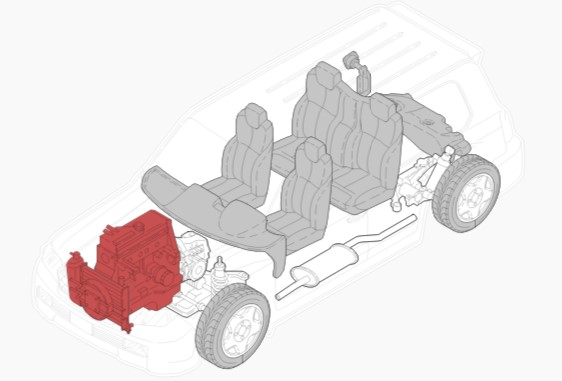
\includegraphics[width=0.65\linewidth]{images/cm1}
	\caption{{\footnotesize {Компоновка \тс. Иллюстрация Audatex}}}
	\label{ris:images/cm1}
\end{figure}
%
\subparagraph*{}
%	
	Согласно заказ-наряду 0000-000194 от 03.08.17, (Т1, л.д. 9) на автомобиле \тс \, в течении одного дня 03.08.2017 специалистами ООО "РЕГИОНТЕХЦЕНТР" выполнены следующие работы:
%	
\begin{table}[H]
			\centering
				\caption{{\footnotesize Выполненные работы и услуги}}
			\label{tab:1}
	\begin{tabular}{|l|l|l|l|}
		\hline
		\rowcolor[HTML]{C0C0C0} 
		\multicolumn{1}{|c|}{\cellcolor[HTML]{C0C0C0}N п/п} & Наименование работ и услуг & Кол-во & Цена, руб \\ \hline
		1                                                   & Диагностика компьютерная   & 1      & 1000      \\ \hline
		\rowcolor[HTML]{EFEFEF} 
		2                                                   & Замер компрессии FSA       & 1      & 1000      \\ \hline
		3                                                   & Снятие/установка форсунок  & 8      & 8000      \\ \hline
		\rowcolor[HTML]{EFEFEF} 
	
	\end{tabular}
\end{table}

Итого на сумму:  37 300 (Тридцать семь тысяч триста) рублей
%
%

\begin{table}[H]
	\centering
	\caption{{\footnotesize Расходы по накладной к заказ-наряду 0000-000194 от 03.08.17}}
	\label{tab:2}
\begin{tabular}{|l|l|l|l|}
			\hline
			\rowcolor[HTML]{C0C0C0} 
			\multicolumn{1}{|c|}{\cellcolor[HTML]{C0C0C0}N п/п} & Наименование запчасти (материала) & Кол-во & Цена, руб \\ \hline
			1                                                   & Шайба под форсунку TOYOTA   & 10      & 2500      \\ \hline
			\rowcolor[HTML]{EFEFEF} 
			2                                                   & Очиститель       & 5     & 1000      \\ \hline
\end{tabular}
\end{table}

Итого на сумму:  3 500 (Три тысячи пятьсот) рублей 

Общая стоимость работ: 40 800 (Сорок тысяч восемьсот) рублей. 
%~\
\vspace{\baselineskip}  % вставка пустой строки

В исковом заявлении (Т1, л.д. 1--6) указано, что после ремонта автомобиля специалистами ООО "РЕГИОНТЕХЦЕНТР"  через непродолжительное время в двигателе автомобиля  \тс \, образовался посторонний, нефункциональный  шум.  Согласно заключения ИП Шаманского С.Н. для устранения неисправности ДВС необходимо было произвести следующие ремонтные работы:

\begin{table}[H]
	\centering
	\caption{{\footnotesize Работы по заказ-наряду № Ш000011955 от 10.08.2017}}
	\label{tab:3}
	\begin{tabular}{|l|l|l|l|}
		\hline
		\rowcolor[HTML]{C0C0C0} 
		\multicolumn{1}{|c|}{\cellcolor[HTML]{C0C0C0}N п/п} & Наименование запчасти (материала) & Кол-во н/ч & Цена, руб \\ \hline
		1    & Материалы, использованные при подготовке а/м к ремонту   & 0,2      & 260      \\ \hline
		\rowcolor[HTML]{EFEFEF} 
		2    & Слесарные работы (ремонт освещения багажного оделения)       & 0,5     & 650    \\ \hline
		3    & Интеркулер снять/установить      & 1     & 1300      \\ \hline
		\rowcolor[HTML]{EFEFEF} 
	
\end{tabular}
\end{table}
Итого на сумму  126 178 (Сто двадцать шесть тысяч сто семьдесят восемь) рублей
% 
 
 \begin{table}[H]
 	\centering
  	\caption{{\footnotesize Запчасти и материалы к заказ-наряду № Ш000011955 от 10.08.2017}}
 	\label{tab:4}
 	\begin{tabular}{|l|ll|l|l|}
 		\hline
 		\rowcolor[HTML]{C0C0C0} 
 		\multicolumn{1}{|c|}{\cellcolor[HTML]{C0C0C0}N кат} & Наименование запчасти (материала) & & Цена за шт. & Всего цена, руб \\ \hline
		7109113821    & Хомут пластиковый самозатяжной  & & 5      & 50      \\ \hline
	    \rowcolor[HTML]{EFEFEF} 
		0411151042    & Ремкомплект ДВС 1VDFTV (1 шт.)      & & 16000     & 16000    \\ \hline
		1111551030С0    & Прогкладка ГБЦ правая  (1 шт.)    & & 3250     & 3250      \\ \hline
		\rowcolor[HTML]{EFEFEF} 
		
 		\end{tabular}
\end{table}
 Итого на сумму  327 203 (Триста двадцать семь тысяч двести три) рубля. \\
 Всего ремонта по справке ИП Шаманского С.Н. на сумму:  397 203 (Триста девяносто семь тысяч двести три ) рубля.
% 
\vspace{\baselineskip}  % вставка пустой строки

Из заключения специалиста  

\vspace{\baselineskip}
%
%
Из заключения экспертов  

\vspace{\baselineskip}
\renewcommand\baselinestretch{0.86}\small\normalsize 
\subsection{\underline{По  вопросу}\, \, \,	\textbf{\small{1. "Опр"?}}}
\renewcommand\baselinestretch{1.2}\small\normalsize
На момент 

 \begin{figure}[H]\centering
	\parbox[t]{0.49\textwidth}
	{\centering
		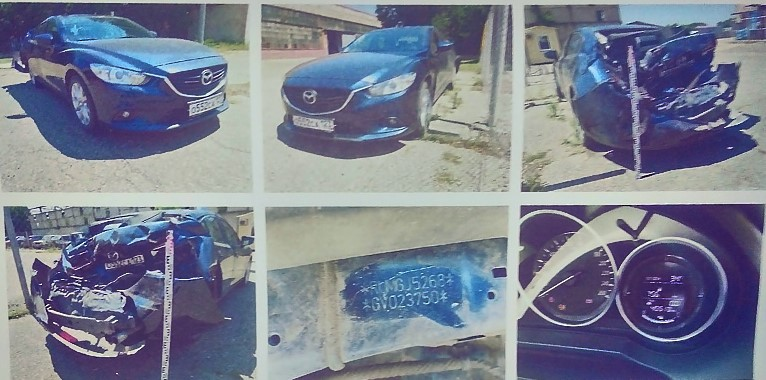
\includegraphics[width=.49\textwidth]{images/k1}
		\caption{\footnotesize {Поврежденное компрессорное колесо (крыльчатка турбины) и его  гайка  }}
		\label{ris:images/k1}}
	\hfil \hfil
	\parbox[t]{0.49\textwidth}
	{\centering
		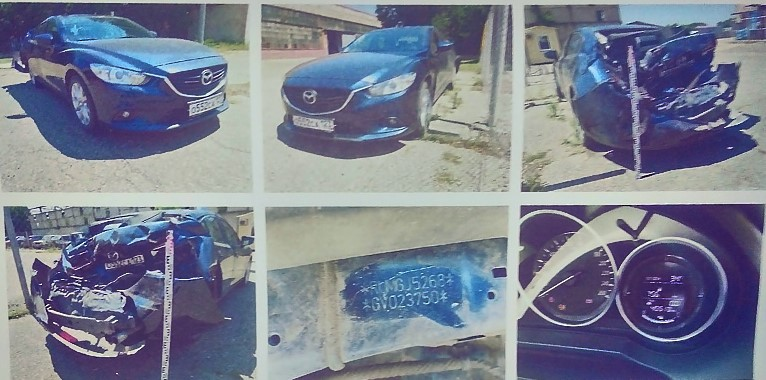
\includegraphics[width=.49\textwidth]{images/k2}
				\caption{\footnotesize {Поврежденное компрессорное колесо (крыльчатка турбины) и стенки корпуса турбины
				рис. 11, 13, Т 1, л.д. 258, 259}}
		\label{ris:images/k2}}
	
\end{figure}

В качестве постороннего предмета истцом заявлен болт клапанной крышки ДВС, извлеченный специалистом ООО "ЭКСПЕРТ",  Рис.\ref{ris:images/b1}
%%
\vspace{\baselineskip}  % вставка пустой строки

  \begin{figure}[!h]
	\centering
	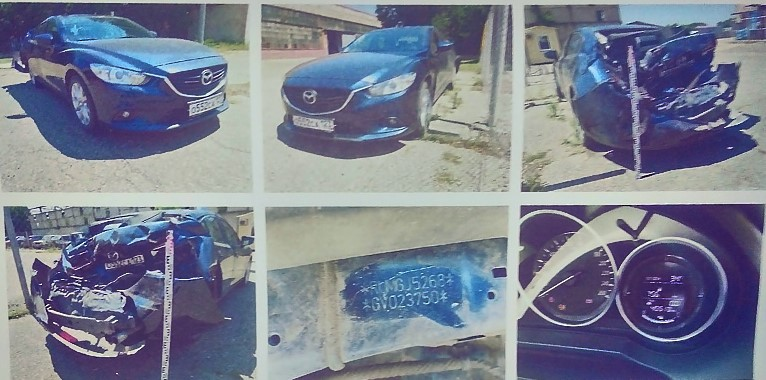
\includegraphics[width=0.95\linewidth]{images/b1}
	\caption{{\footnotesize {Поврежденный болт клапанной крышки, основан на Рис. 12, Т 1, л.д. 258}}}
	\label{ris:images/b1}
\end{figure}

%   \begin{figure}[!h]
%	\centering
%	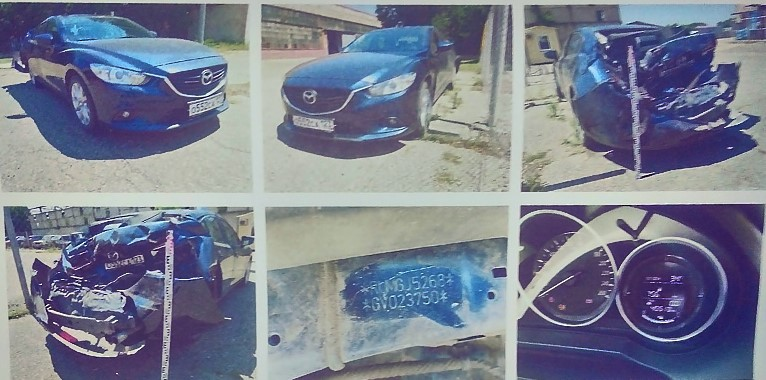
\includegraphics[width=0.85\linewidth]{images/b2}
%	\caption{{\footnotesize {Поврежденный болт клапанной крышки, вид с торца. Левая стрелка указывает на наклеп шляпки болта, правая- на повреждения торца резьбы детали}}}
%	\label{ris:images/b2}
%\end{figure}


\begin{figure}[!h]\centering
	\parbox[t]{0.49\textwidth}
	{\centering
		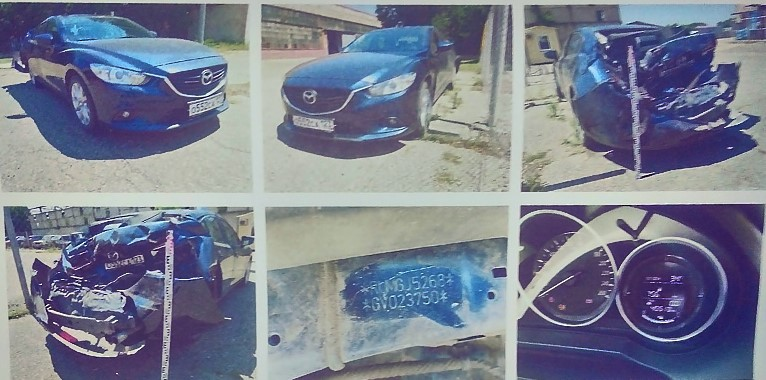
\includegraphics[width=.49\textwidth]{images/b2}
		\caption{\footnotesize {Поврежденный болт клапанной крышки, вид с торца. Левая стрелка указывает на наклеп шляпки болта, правая- на повреждения торца резьбы детали }}
		\label{ris:images/b2}}
	\hfil \hfil
	\parbox[t]{0.49\textwidth}
	{\centering
		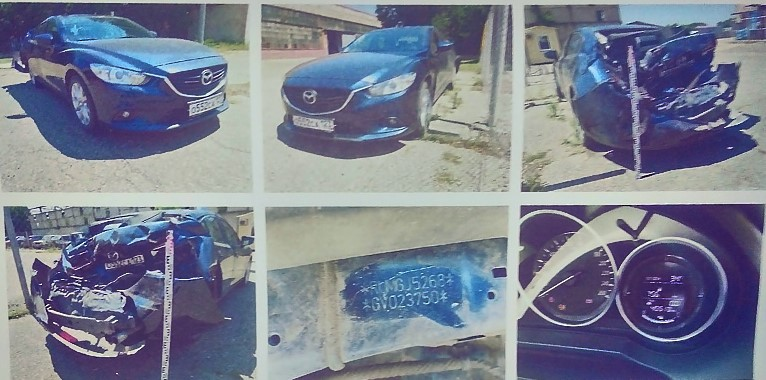
\includegraphics[width=.49\textwidth]{images/g1}
		\caption{\footnotesize {Поврежденная гайка  компрессорного колеса (крыльчатки турбины)
				рис. 11, 13, Т 1, л.д. 258, 259}}
		\label{ris:images/g1}}
	
\end{figure}
%\begin{SCfigure}
%	\centering {\footnotesize \caption{Болт клапанной крышки, извлеченный из впускного тракта }} 
%	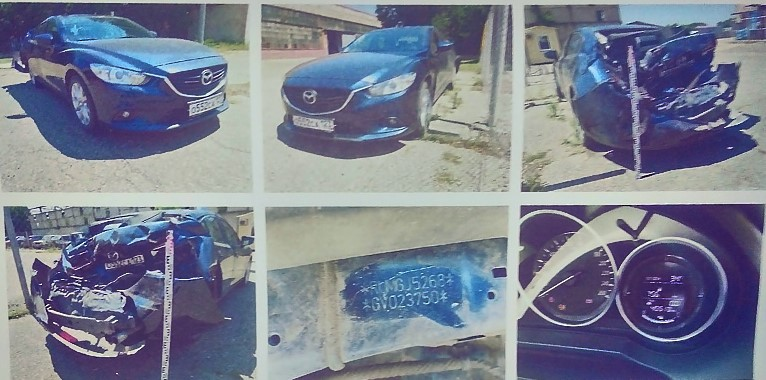
\includegraphics[]{images/b1}
%	\label{ris:images/b1}
%\end{SCfigure}


Эксперты ИП 
%

Из материалов дела следует, что .


\relax
\begin{figure}[h!]\centering
	\parbox[t]{0.49\textwidth}
	{\centering
		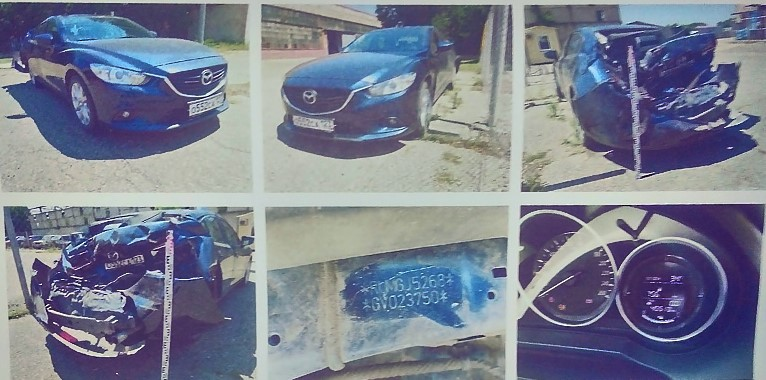
\includegraphics[width=.49\textwidth]{images/b3}
		\caption{\footnotesize {Сформированная фаска галтели поврежденного болта}}
		\label{ris:images/b3}}
	\hfil \hfil
	\parbox[t]{0.49\textwidth}
	{\centering
		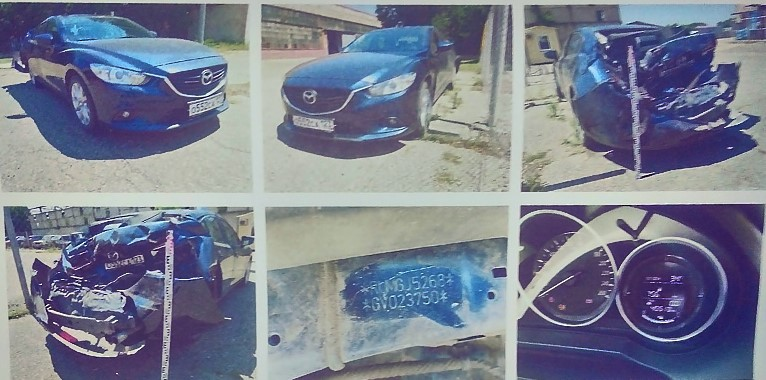
\includegraphics[width=.49\textwidth]{images/b4}
		\caption{\footnotesize {Галтели неповрежденных болтов выраженных 
				фасок не имеют}}
		\label{ris:images/b4}}
\end{figure}

По совокупности результатов
\subparagraph*{}Таким образом, по совокупности признаков, эксперт приходит вероятностному  выводу о том, что повреждения колеса турбины (крыльчатки компрессора турбокомпрессора) могли быть образованы вследствие попадания постороннего предмета, а именно болта крышки клапанов, извлеченного специалистом ООО "ЭКСПЕРТ". 

\subparagraph*{}  Экспертами 


% 
%\begin{flushleft} 
% 	\hbox{% 
% 		\vrule\hspace{.8em}\parbox{1\textwidth}% 
% 		{ Согласно руководству по сервисному обслуживанию и ремонту TOYOTA LAND CRUISER 200 для проведения работ в объёме, указанном в заказ-наряде №0000-000194 от 03.08.2017 г. (л.д.9), составленном специалистом ООО «РЕГИОНЦЕНТР» (г. Краснодар) необходимо демонтировать агрегаты, находящиеся в пространстве между двигателем и передней панелью, в том числе патрубок подвода воздуха к компрессору левого турбокомпрессора исследуемого двигателя (где в дальнейшем был обнаружен такой посторонний предмет как крепёжный болт).}} 
%\end{flushleft}
% 
% 
\subsection{Исследование транспортного средства}
%
Осмотр автомобиля производился экспертом в условиях дилерского сервисного центра в г. Краснодаре, ул. Аэропортовская, 4/1. При проведении осмотра присутствовали: \присутствовали. \\
Автомобиль предоставлен частично разобранным: демонтирован поддон двигателя, вкладыши коленчатого вала, шатунные катушки зажигания, свечи зажигания.  Отдельно представлена пластиковая емкость, содержащая 3 литра масла из двигателя ТС \тс.
На момент осмотра на автомобиле имеются повреждения переднего бампера снизу слева в виде задиров, крыло заднее правое  имеет царапины ЛКП, бампер задний справа имеет царапины ЛКП, имеется повреждение лобового стекла. Давление в шинах колес передней и задней оси 2.3 бар, шины BRIDGESTONE TURA NZA 225/55R17 97V
%%      
%% \textbf{  Повреждения автомобиля \tcm,\, имеющиеся на момент осмотра 02.07.2018:} (рис. \ref{fig:merclz}, \ref{fig:51})  %\rem{Описания повреждений автомобилей}
%   \begin{itemize}{}{}
% 	 \vspace{-2mm}
%\subparagraph{title}
%\item Дверь передняя левая - компрессионная деформация  поверхности панели, деформация каракаса детали. В средней части лицевой панели, на площади $ \approx 1\, \text{дм}^2 $ глубокая вмятина с участками разрыва металла,   образованная в направлении снизу вверх и слева направо, ниже молдинга статический след  предмета прямоугольной формы  $ \approx 10$ x $20\, \text{см} $; 
%\item Молдинг двери передней левой - деформирован; 
%
% \end{itemize}   
%
%\vfill
%\begin{figure}[!h]
%	\centering
%	\includegraphics[width=0.85\linewidth]{images/51}
%	\caption{{\footnotesize Левая передняя часть автомобиля \tcm. Стрелки указывают на повреждения передней левой  части автомобиля}} \vspace{10mm} 
%	\label{fig:51}
%\end{figure}
%\vspace{5mm} 
%
%\textbf{Исследование повреждений ходовой части} проводилось с использованием ручного измерительного инструмента и стенда для измерения углов установки колес. 
%\begin{SCfigure}
%	\centering {\footnotesize \caption{ Автодата. Схема рычагов задней подвески }} 
%	\includegraphics[width = 0.4 \textwidth] % 
%	{images/p1} % picture filename 
%\end{SCfigure}
%\begin{SCfigure}
%	\centering {\footnotesize \caption{ Подвеска автомобиля \tcm\, левая повреждённая сторона. Стрелками показаны  деформированные рычаги }} 
%	\includegraphics[width = 0.4 \textwidth] % 
%	{images/50} % picture filename 
%\end{SCfigure}
%\relax
%\begin{figure}[h!]\centering
%	\parbox[t]{0.49\textwidth}
%	{\centering
%		\includegraphics[width=.49\textwidth]{images/p1}
%		\caption{\footnotesize {Автодата. Схема рычагов задней подвески}}
%		\label{fig:p1}}
%	\hfil \hfil
%	\parbox[t]{0.49\textwidth}
%	{\centering
%		\includegraphics[width=.49\textwidth]{images/50}
%		\caption{\footnotesize { Подвеска автомобиля \tcm\, левая повреждённая сторона. Стрелками показаны  деформированные рычаги }}
%		\label{fig:50}}
%\end{figure}
%\begin{figure}[h!]\centering
%	\parbox[t]{0.49\textwidth}
%	{\centering
%		\includegraphics[width=.49\textwidth]{images/47}
%		\caption{\footnotesize {Измерение углов установки колес}}
%		\label{fig:47}}
%	\hfil \hfil
%	\parbox[t]{0.49\textwidth}
%	{\centering
%		\includegraphics[width=.49\textwidth]{images/48}
%		\caption{\footnotesize { Экран стенда измерения углов установки колес }}
%		\label{fig:48}}
%\end{figure}
%%
%\begin{figure}[h!]
%	\centering
%	\includegraphics[width=0.9\linewidth]{images/50}
%	\caption[]{{\footnotesize Подвеска автомобиля \tcm\, левая повреждённая сторона. Стрелками показаны  деформированные рычаги}}
%		\label{fig:50}
%\end{figure}
%
%
%
%\begin{figure}[h!]
%	\centering
%	\includegraphics[width=0.85\linewidth]{images/50}
%	\caption[]{{\footnotesize Подвеска автомобиля \tcm\, левая повреждённая сторона. Стрелками показаны  деформированные рычаги}}
%	\label{fig:50}
%\end{figure}
%
%\vspace{10mm}
%   
% \subparagraph*{}\textbf{На предоставленном автомобиле} \tcm\  на момент осмотра раскрыты левая передняя боковая подушка безопасности и левая головная подушка безопасности, Рис. \ref{fig:52}. Система оконных подушек безопасности входит в базовую
% комплектацию модельного ряда W211. Оконные и боковые подушки безопасности срабатывают в том  случае, если центральный электронный блок управления ARMADA регистрирует боковое столкновение. Для определения поперечного  ускорения поступающая от центрального датчика столкновения  информация дополняется информацией от боковых датчиков,
% расположенных в зонах боковых поперечин соответствующих  сторон.
% 
% В результате произведенной проверки электрических цепей системы SRS на наличие повреждений, коррозии, нарушения контактов в   разъемных соединениях  неисправности проводки электрических цепей системы SRS не выявлено. Блок управления системы безопасности в реальном времени нормально реагирует на внешние тестовые воздействия.
% \vspace{3mm}
%\begin{figure}[!h]
%	\centering
%	\includegraphics[width=0.85\linewidth]{images/52}
%	\caption{{\footnotesize Автомобиль \tcm с раскрытыми надувными элементами подушек безопасности}}
%	\label{fig:52}
%\end{figure}
%
На автомобиле имеются характерные повреждения 

% \begin{figure}
% 	\centering
% 	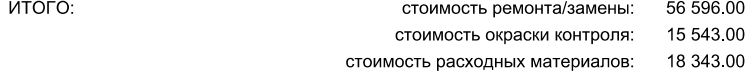
\includegraphics[width=0.95\linewidth]{images/screenshot001}
% 	\caption{{\footnotesize Данные блока управления панели комбинации приборов, зафиксированные в процессе исследования автомобиля}}
% 	\label{fig:screenshot001}
% \end{figure}
% \vspace{5mm}
% \begin{figure}[!h]
% 	\centering
% 	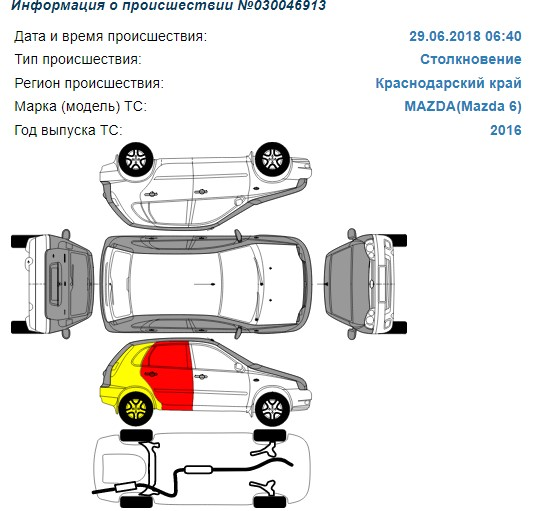
\includegraphics[width=0.95\linewidth]{images/d1}
% 	\caption{\footnotesize Снимок экрана компьютера в процессе диагностики системы управления} 	\label{fig:d1}
% \end{figure}
%{\small \begin{enumerate}{\label{en:enum}}
%		\item [] Ошибки системы SRS:
%	\item 92A3 - высокое сопротивление запального контура левой оконной подушки безопасности. Начало ошибки -- ошибка снята: 19 109 126 мотосекунда -- 19 138 962 мотосекунда или 5 308,09 моточасов -- 5 316,37 моточасов);
%	\item 9223 - высокое сопротивление запального контура левой боковой подушки безопасности: 19 109 126 --33 554 430 мотосекунд или 5 308,09 -- 9 320,67 моточасов;
%	\item 92А0 - замыкание (или утечка)на массу в цепи левой оконной подушки безопасности:  19 138 964-- 33 554 430 мотосекунд или  5 316,37 --9 320,67 моточасов.
%\end{enumerate}}
%
%\vspace{-14mm}
%\begin{center}
%	%\renewcommand{\arraystretch}{0.8}ommand{\arraystretch}{0.8}
%%\begin{tabular}{|p{20mm}|p{7cm}|p{25mm}|p{25mm}|}
%%	\hline 
%%	{\footnotesize Код ошибки} & {\footnotesize Описание ошибки} & {\footnotesize Время возникновения, сек} &{\footnotesize  Время окончания, сек} \tabularnewline
%%	\hline 
%%	92A3 & {\small Высокое сопротивление запального контура оконной подушки безопасности} & 19109126 & 19138962 \tabularnewline
%%	\hline 
%%	9233 & {\small Высокое сопротивление запального контура боковой подушки безопасности} & 19109126 & 3355430 \tabularnewline
%%	\hline 
%%	92A0 & {\small Замыкание  в цепи левой оконной подушке безопасности} & 19138964 & 33554430 \tabularnewline
%%	\hline 
%%%	\label{t:pb}
%%\end{tabular}
%%\renewcommand{\arraystretch}{1.2}
%%\begin{tabular}{|p{20mm}|p{7cm}|p{25mm}|p{25mm}|}
%%	\hline 
%%	{\footnotesize Код ошибки} & {\footnotesize Описание ошибки} & {\footnotesize Время возникновения, сек} &{\footnotesize  Время окончания, сек} \tabularnewline
%%	\hline 
%%	92A3 & {\small Высокое сопротивление запального контура оконной подушки безопасности} & 19109126 & 19138962 \tabularnewline
%%	\hline 
%%	9233 & {\small Высокое сопротивление запального контура боковой подушки безопасности} & 19109126 & 3355430 \tabularnewline
%%	\hline 
%%	92A0 & {\small Замыкание  в цепи левой оконной подушке безопасности} & 19138964 & 33554430 \tabularnewline
%%	\hline 
%%%	\label{t:pb}
%%\end{tabular}
%%\renewcommand{\arraystretch}{1.2}}
%\end{center}
%\vspace{3mm}
%Высокое электрическое сопротивление цепи запального контура указывает на активацию газогенератора (пиропатрона). По данным блока SRS, активация газогенераторов обеих подушек безопасности произошла одновременно на 19109126 мотосекунде.  Снятие ошибки 92А3 совпадает (разница 2 секунды) с моментом возникновения ошибки 92А0 (одновременно с образованием замыкания на массу в цепи левой оконной подушки). Т.е. неисправность электрической цепи  системы управления головной подушкой безопасности в виде короткого замыкания или утечки на массу зафиксировано на 8 часов позднее, чем произошла активация системы SRS и, согласно этим данным, не может являться причиной нештатного раскрытия надувного элемента головной подушки.    
%Считанные показания счетчика моточасов работы из блока управления панели приборов -- 53 19,02 ч. или $ \approx 19 148 472 $ мотосекунды, при том, что в блоке SRS содержатся сведения о снятии ошибки на 33 554 430 мотосекунде или 9 320,67 моточасе  работы автомобиля, что есть существенное расхождение во времени работы автомобиля  в различных блоках управления.  Показания одометра на 10.11.2017г. составляли 89 855 км, (акт осмотра ИП Резенькова, л.~д. 30), показания одометра на момент настоящего исследования так же 
%89 855км. Данный факт указывает либо на вмешательство в  блоки управления автомобиля, либо на наличие неисправных блоков управления.  Таким образом, техническое состояние электрических систем исследуемого автомобиля на момент экспертизы не позволяет достоверно определить соответствие срабатывания боковых подушек безопасности заявленному ДТП \dtp.  
%\subsection*{}
%%\vspace{-10mm}
%\vspace{-10mm}\textbf{  Повреждения автомобиля \tca,\, имеющиеся на момент осмотра 02.07.2018:}   
%
%\begin{itemize}
%	
%	\item Капот - остаточная деформация передней части,\, деталь частично восстановлена; 
%	\item Фара левая - заменена;
%	\item Фара правая - разрушен корпус;
%	\item Бампер передний - расколот в левой части, остаточные признаки пластической деформации правой части детали, отслоение ЛКП; 
%	\item Фара правая противотуманная - разбита;
%	\item Облицовка передняя - деформирована;
%	\item Панель рамки радиатора - частично восстановлена геометрия, имеются остаточные деформации;
%	\item Лонжероны передние левые - имеют остаточные деформации передней части деталей;
%	\item Пластина переднего регистрационного знака - деформирована;
%	\item Крыло переднее левое - остаточная деформация, разрывы металла передней угловой части;
%	\item Крыло переднее правое - остаточная деформация, разрывы металла передней угловой части.\\
%	
%\end{itemize}
%\imgh{150mm}{images/38}{Автомобиль \tca\, вид спереди. Расстояние между передними крыльями 1310 мм. Передний верхний угол левого и правого крыла расположены на высоте  720 мм от опорной поверхности.}
%
%\imgh{165mm}{images/mercl}{Автомобиль \tcm\, левая боковина. Расстояние между повреждениями 1310 мм. Расположены на высоте 620...680 мм и 610...670 мм} 
%
%  	Следуя логической последовательности разрешения вопросов настоящей экспертизы,     первоначально необходимо установить механизм взаимодействия автомобилей при заявленных обстоятельствах,  исследовать повреждения транспортных средств,   произвести сопоставление имеющихся повреждений с  механизмом их образования, определить возможность образования повреждений при заявленном событии и только затем определить стоимость восстановительного ремонта повреждений автомобиля \tcm.  Таким образом, эксперт первоначально должен провести  исследование по второму вопросу.
%  
%  \renewcommand\baselinestretch{0.85}\small\normalsize 
% \subsection{\underline{По  вопросу}\, \, \,	\textbf{\small{2. Состоят ли в причинно-следственной связи повреждения транспортного средства Мерседес Бенц регистрационный знак Р781ЕХ93 2003 года выпуска, заявленного истцом с ДТП, имевшем место 31.10.2017г.?}}}  
% \renewcommand\baselinestretch{1.2}\small\normalsize
% 
% %\vspace{-10mm}
%\subparagraph*{}	\parindent=2em  В соответствии с теорией автомобиля и законами механики, взаимодействие  транспортных средств возможно  определёнными зонами	 контактирования на площади перекрытия в вертикальных и горизонтальных плоскостях, исходя из конструктивных особенностей компоновки кузова при геометрическом ориентировании на проезжей части. Соответственно,  образование повреждений на транспортных средствах возможны  в  закономерных направлениях – в продольном направлении: спереди назад или сзади вперёд; в поперечном направлении: слева направо или справа налево;  в комбинированных направлениях при определённых условиях взаимодействия, исходя из особенностей динамики перемещения: спереди назад и сверху вниз, спереди назад и снизу вверх; сзади вперед и сверху вниз; сзади вперед и снизу вверх. Определение механизма столкновения транспортных средств\footnote{С.Я. Евтюков, Я.В. Васильев\,/ Экспертиза ДТП: Методы и технологии/ СПбГАСУ.-Спб., 2012.-310с. ISBN 978-5-9227-0426-7} включает в себя установление траекторий схождения и расхождения транспортных средств; угла между продольными осями транспортных средств в момент их первичного контактного взаимодействия; частей транспортных средств, которыми они впервые вступили в контактное взаимодействие; площади перекрытия контактирующих при ДТП частей транспортных средств; факта состояния покоя или движения транспортных средств в момент первичного контактного взаимодействия; координат места столкновения и расположения транспортных средств относительно неподвижных элементов дороги.% Механизм столкновения устанавливается по следам на транспортных средствах и месте ДТП. Взаимное положение транспортных средств в момент первичного контактного взаимодействия определяется методом натурной реконструкции события ДТП (совмещение и сопоставление пар повреждений на транспортных средствах участвовавших в ДТП) либо при отсутствии такой возможности, по протоколам осмотра транспортных средств и фотографиям их повреждений, приобщенным к материалам дела. По удовлетворению ходатайства \hod транспортные средства на исследование представлены, что позволило эксперту провести натурную реконструкцию взаимодействия транспортных средств, в соответствии заявленному механизму  ДТП. %Установленный механизм взаимодействия автомобилей \tca и \tcm  не противоречит заявленным обстоятельствам ДТП и соответствует условиям перекрестного поперечного столкновения, обусловленного пересечением траекторий движения автомобилей.\,Проведённой в процеcсе исследования натурной реконструкцией столкновения представленных автомобилей   установлено, что правая боковая сторона автомобиля мерседес--бенц Е220  гос.рег.знак Р781ЕХ93 содержит  следы--отображения внешнего строения деталей передней части автомобиля ауди--80 регистрационный знак В393НУ12.
%\vspace{-10mm}
% \subsection*{}
%      \textbf{В результате детального изучения следов на предоставленных ТС  эксперт выделяет следующие контактные пары:}
%\vspace{2mm}
%%\begin{itemize}
%	\item рамка переднего номерного знака \tca и дверь задняя левая \tcm, рис. \ref{ris:images/11}, \ref{ris:images/13}.
%	\item  левая сторона переднего бампера с отверстием  для противотуманной фары  \tca --- дверь передня левая \tcm, рис. \ref{ris:images/46}, \ref{ris:images/32}.
%	\item повреждение левой передней двери \tcm, полученное от контактного взаимодействия с левым передним крылом \tca, рис. \ref{ris:images/35}, \ref{ris:images/36}.
%	\item повреждение левого заднего крыла \tcm, полученное от контактного взаимодействия с правым передним крылом \tca, рис. \ref{ris:images/33}, \ref{ris:images/34}.
%	\item повреждения левой передней и левой задней двери \tcm компрессионного характера - передний бампер ТС, капот, левая и правая фары \tca, рис. \ref{ris:images/37}, \ref{ris:images/38}. 
%	
%\end{itemize}
%\relax
%\begin{figure}[h!]\centering
%	\parbox[t]{0.49\textwidth}
%	{\centering
%		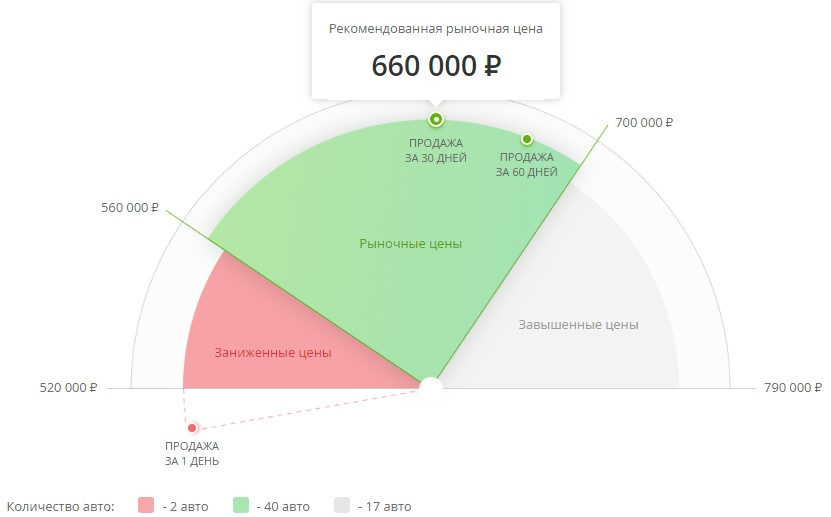
\includegraphics[width=.49\textwidth]{images/1}
%		\caption{\footnotesize {Этапы реконструкции ДТП}}
%		\label{ris:images/1}}
%	\hfil \hfil%раздвигаем боксы по горизонтали 
%	\parbox[t]{0.49\textwidth}
%	{\centering
%		\includegraphics[width=.49\textwidth]{images/39}
%		\caption{\footnotesize {Этапы реконструкции ДТП}}
%		\label{ris:images/39}}
%\end{figure}
%\relax
%\begin{figure}[h!]\centering
%	\parbox[t]{0.49\textwidth}
%	{\centering
%		\includegraphics[width=.49\textwidth]{images/11}
%		\caption{\footnotesize {След рамки номерного знака}}
%		\label{ris:images/11}}
%	\hfil \hfil%раздвигаем боксы по горизонтали 
%	\parbox[t]{0.49\textwidth}
%	{\centering
%		\includegraphics[width=.49\textwidth]{images/13}
%		\caption{\footnotesize {След воздействия правого переднего крыла автомобиля \tca на поверхность крыла заднего левого автомобиля \tcm}}
%		\label{ris:images/13}}
%\end{figure}
%\relax
%\begin{figure}[h!]\centering
%	\parbox[t]{0.49\textwidth}
%	{\centering
%		\includegraphics[width=.49\textwidth]{images/46}
%		\caption{\footnotesize {левая сторона переднего бампера с отверстием  для противотуманной фары  \tca}}
%		\label{ris:images/46}}
%	\hfil \hfil%раздвигаем боксы по горизонтали 
%	\parbox[t]{0.49\textwidth}
%	{\centering
%		\includegraphics[width=.49\textwidth]{images/32}
%		\caption{\footnotesize {дверь передня левая \tcm}}
%		\label{ris:images/32}}
%\end{figure}
%\relax
%\begin{figure}[h!]\centering
%	\parbox[t]{0.49\textwidth}
%	{\centering
%		\includegraphics[width=.49\textwidth]{images/35}
%		\caption{\footnotesize {Левая передняя дверь автомобиля  \tcm}}
%		\label{ris:images/35}}
%	\hfil \hfil%раздвигаем боксы по горизонтали 
%	\parbox[t]{0.49\textwidth}
%	{\centering
%		\includegraphics[width=.49\textwidth]{images/36}
%		\caption{\footnotesize {Левое переднее крыло автомобиля \tca}}
%		\label{ris:images/36}}
%\end{figure}
%
%\relax
%\begin{figure}[h!]\centering
%	\parbox[t]{0.49\textwidth}
%	{\centering
%		\includegraphics[width=.49\textwidth]{images/33}
%		\caption{\footnotesize {Левое заднее крыло автомобиля \tcm}}
%		\label{ris:images/33}}
%	\hfil \hfil%раздвигаем боксы по горизонтали 
%	\parbox[t]{0.49\textwidth}
%	{\centering
%		\includegraphics[width=.49\textwidth]{images/34}
%		\caption{\footnotesize {Левое переднее крыло автомобиля \tca}}
%		\label{ris:images/34}}
%\end{figure}
%\relax
%\begin{figure}[h!]\centering
%	\parbox[t]{0.49\textwidth}
%	{\centering
%		\includegraphics[width=.49\textwidth]{images/37}
%		\caption{\footnotesize {Левые двери автомобиля \tcm. Следовоспринимающая поверхность}}
%		\label{ris:images/37}}
%	\hfil \hfil%раздвигаем боксы по горизонтали 
%	\parbox[t]{0.49\textwidth}
%	{\centering
%		\includegraphics[width=.49\textwidth]{images/23}
%		\caption{\footnotesize {Передний бампер, капот, левая и правая фары \tca. Следообразующая поверхность}}
%		\label{ris:images/23}}
%\end{figure}
%%\rem{Возможно, необходимо перенести в другой раздел}
%\subparagraph*{} Имеющиеся следы комбинированные, статические, направленные перпендикулярно продольной оси автомобиля \tcm с незначительной динамической составляющей  следов внедрения, направленные снизу вверх  и немного слева направо (под углом $ \approx 30^{\circ} $) к вертикальной оси автомобиля.%  рис. \ref{ris:images/1}, \ref{ris:images/39}. \rem{фото характерных следов}
%
%Совокупность индивидуализирующих признаков групп следов и повреждений, имеющихся  на транспортных средствах, совпадающих между собой по уровню расположения, форме и  локализации указывают на   возможность их образования при взаимном контактном взаимодействии по механизму перекрёстного взаимодействия  с центральным ударом.  Различие по высоте ($ \approx 9  \cdots 10 $ см ), в данном случае,  не противоречит  механизму следообразования, так как  закономерность направления деформирующего воздействия со стороны следообразующего объекта на части кузова транспортного средства обусловлены  геометрическими размерами  рассматриваемых объектов, траекторией их перемещения, а также созданием определенных моментов сил,  в том числе вызывающих перераспределение массы по осям, рис.27\ref{ris:images/tormoz}.   Полагаем, что водитель автомобиля \tca, \, перед столкновением с автомобилем \tcm, применил торможение.  Тогда в  момент первичного контакта передняя часть автомобиля  \tca \ была расположена на несколько сантиметров ниже относительно расстояния при нормальных условиях движения или неподвижного состояния, так как согласно законам механики,  в момент торможения происходит перераспределение веса под действием силы
%  \begin{equation}\label{eq:f}
%  \vec{F_t} = \dfrac{\vec{a}*m*H}{L}, \,\,\,\,  \text{где:}
%  \end{equation}
%  \begin{itemize}
%  \item[ ] $\vec{a} $ ---величина замедления;
%  \item[ ] $ L $ --- длина базы автомобиля;  
%  \item[ ] $ H $ --- высота центра тяжести; 
%   \item[ ] $ m $ --- масса автомобиля
%  \end{itemize}
% Действие силы $ \vec{F_t} $   на переднюю ось автомобиля  приводит к дополнительному сжатию пружин передней подвески и, как следствие, уменьшению расстояния от деталей передней части кузова до опорной поверхности. Величина уменьшения расстояния зависит от значения силы $ \vec{F_t} $ и жёсткости  подвески автомобиля.
%В свою очередь,  в начальный момент контакта, положение кузова автомобиля \tcm \, должно было  соответствовать  положению при нормальном  условии движения, далее, под действием силы $ \vec{F_t} = \dfrac{mv^2}{2} $ , где $ m $ -- масса автомобиля \tcm, v -- его скорость, пространственное положение кузова \tcm измениться.
%\imgh{100mm}{images/torm}{Схематичное изображение перераспределения веса при торможении автомобиля }
%\begin{SCfigure}
%\centering \caption{рлрл captioорпоп опрпоп опорпопр опопо  порпорп орор оро опрорп орп ор оорп орп оn text ... } 
%\includegraphics[width = 0.6 \textwidth] % 
%{images/torm} % picture filename 
%\end{SCfigure}
%Анализ характера деформаций и направлений действующих сил, вызвавших повреждения частей деталей правой боковины автомобиля \tcm \, и передней части автомобиля \tca, а именно:
%\begin{itemize}
%	\item[ ] --  обширные площади деформации на ТС в местах, которыми они вошли в контактное взаимодействие с преградой;
%	\item[ ] --  оттиски отдельных участков, деталей одного ТС на поверхности частей другого;
%	\item[ ] --  следы внедрения в виде потёртостей на ТС -- снятия слоя лакокрасочного покрытия, локальных разрывов поверхности;
%	\item[ ] -- трассы (следы скольжения, давления, царапания), возникшие от контакта с другим ТС
%\end{itemize} 
%позволяют заключить, что данные повреждения могли быть образованны в результате  взаимного контактного взаимодействия указанных автомобилей.\\
%Данный механизм следообразования является характерным для \rem{вставить механизм следообразвания}
%Таким образом, сопоставлением характерных групп следов, местом и направлением их нанесения, пространственным совмещением выделенных следовоспринимающих и следообразующих объектов можно сделать общий вывод о наличии пространственно-следового изоморфизма, и соответственно о наличии контактно-следового взаимодействия автомобилей \tca и \tcm.
%
%	Учитывая заявленные обстоятельства ДТП \dtp, исходя из взаимного ориентирования обоих транспортных средств на проезжей части  соответствующими сторонами кузова, а также направления траектории сближения обоих транспортных средств по принципу организации дорожного движения, повреждения левой боковой части автомобиля \tcm могут состоят в причинно-следственной связи с указанным  ДТП. 
%Повреждения деталей передней части автомобиля \тсм, согласно предоставленным административных материалов по данному ДТП, получены в результате наезда автомобиля на дерево, расположенное  на расстоянии 4,6 м от края проезжей части и на удалении $ \approx 10 $ м от места столкновения автомобилей, рис.2. 
%На момент исследования, на автомобиле \тсм имеются остаточные признаки упругой деформации деталей передней левой части автомобиля, по совокупности морфологических признаков не противоречащие заявленному механизму образования. Положение автомобиля \тсм, указанное на схеме ДТП, должно быть обусловлено изменением траектории движения автомобиля после столкновения на угол, составляющий $ \approx 40^\circ $ вправо от направления  движения до столкновения автомобилей. При этом, схема места дорожно-транспортного происшествия не содержит следов потери устойчивости автомобиля после столкновения. Из  анализа механизма взаимодействия автомобилей, эксперт приходит к заключению, что положение автомобиля \тсм, указанное  на схеме ДТП не является результатом изменения траектории его  движения  вследствие удара, а вероятно, связано с управляющими действиями водителя, его ответной реакцией на столкновение.
%Следовательно, повреждения деталей передней части автомобиля \tcm могут находится в причинно-следственной связи с указанным  ДТП.% так как  характер повреждений  не противоречит заявленным обстоятельствам. 
%\subparagraph*{}Таким образом, по совокупности признаков, эксперт приходит к выводу о том, что  повреждения транспортного средства Мерседес Бенц регистрационный знак Р781ЕХ93 2003 года выпуска  состоят  в причинно-следственной связи с  ДТП, имевшем место 31.10.2017г.
%{\begin{enumerate}
%		
%	\item Наличие чётких отпечатков частей одного ТС на другом в местах их первичного контакта при отсутствии трасс местах образования отпечатков или при наличии трасс, возникших после образования отпечатков \rem{еще ремарка по ударв неподвижное тс}
%	\item  Совпадение направления первоначальных трасс и деформаций на ТС, по которому был нанесен удар при перекрёстном столкновении,  направлением движения другого ТС
%	\item Расположение трасс тангенциальной направленности на боковой поверхности колес
%	\item Разворот ТС в направлении момента, который мог возникнуть при столкновении только в случае движения тс, по которому был нанесён удар \\
%	
%	 
%\end{enumerate}}
%Необходимо отметить \rem{опять про изоморфизм}, что данный вид трасологических исследований (установление пространственно-следового изоморфизма, а
%именно установление факта контактно-следового взаимодействия,
%сопоставление обстоятельств ДТП, заявленных страхователем с механизмом нанесения повреждений и т.д.) в настоящее время становится все более и более востребованным и актуальным, т.к. в современных условиях складывается ситуация, когда мошенничество на
%транспорте, с целью получения страхового возмещения, приобретает объёмы снежного кома.
%%%%%%%%%%%%%%%%%%%%%%%%%%%%%%%%%%%%%%%%%%%%%%%%%%%%%%%%%%%%%%%%%%%%%%%%%%%%%%%%%%%%%%%%%%%%%%%%%%%%%%%%%%%%%%%%%%%%%%%%%%%%%
\renewcommand\baselinestretch{0.86}\small\normalsize 
\subsection{\underline{По  вопросу}\, \, \,	\textbf{\small{"Определить стоимость восстановительного ремонта с учетом износа стоимости запасных частей"?}}}
\renewcommand\baselinestretch{1.2}\small\normalsize
Колесное транспортное средство сроком эксплуатации более 7 лет относится к категории транспортных средств с граничным сроком эксплуатации [1], для которой возможно применение ремонтных операций при условии экономической целесообразности и  технической возможности.  
                                         
В соответствии с принятой экспертной методикой [1], стоимость восстановительного ремонта АМТС  $ C_p $ определяется по формуле:
%
\begin{equation}\label{eq:r}
C_\text{вp} =C_p + C_\text{м} + C_\text{зч}\cdot\left( 1-\frac{\text{И}}{100}\right)  \,\,\,\, \text{где:}
\end{equation}
%
%
\begin{itemize}
%	
\item[ ]$C_\text {р} $ --  стоимость ремонтных работ по восстановлению КТС, руб.;
\item[ ]$ C_\text{м} $ --  стоимость необходимых ремонтных материалов, руб.;
\item[ ]$ C_\text{зч} $ --  стоимость новых запасных частей, руб;
\item[ ] $ \text{И} $ -- коэффициент износа составной части, подлежащей замене, \%.
\end{itemize}
%
%
Коэффициент износа составных частей (И) КТС (кроме автобусов и грузовых автомобилей) при определении стоимости восстановительного ремонта расчитывается по формуле:

\begin{equation}\label{eqsnos}
\text{И} =\text{И1}\cdot\text{П}+\text{И2}\cdot \text{Д}, \%  \,\,\,\, \text{где:}
\end{equation}

\begin{itemize}
	\item [] $ \text{И1} $ --усредненный показатель износа на 1000 км пробега, \%; 
	\item [] $ \text{П} $ -- общий пробег (фактический или расчетный) за срок эксплуатации КТС, тыс.км;
	\item [] $ \text{И2} $ -- усредненный показатель старения за 1 год эксплуатации, \%;
	\item [] $ \text{Д} $ -- срок эксплуатации КТС (от даты изготовления КТС до момента, на который определяется износ), лет. 
\end{itemize}

Для исследуемого автомобиля \тс, согласно справочным таблицам [1]:
\begin{equation}\label{eqsnosr}
\text{И} =\text{И1}\cdot\text{П}+\text{И2}\cdot \text{Д} = 0.23\cdot 214  + 0.85\cdot 9 = 49 \, \%
\end{equation}
%%%%%%%%%%%%%%%%%%%%%%%%%%%%%%%%%%%%%%%%%%%%%%%%%%%%%%%%%%%%%%%%%%%%%%%%%%%%%%%%%%%%%%%%%%%%%%%%%%%%%%%%%%%%%%%%
%Стоимость восстановительных работ $ C_{\text{вр}} $ определяется на основании норм трудоёмкостей $ T_i $, \,предусмотренных заводом-изготовителем, и стоимостных параметров $ C_{i\text{нч}} $ (стоимости нормо-часа) работ по техническому обслуживанию и ремонту АМТС. 
%\begin{equation}\label{eq:cr}
%C_{\text{вр}}  =\sum{C_{ip}}= \sum\left({T_{ij}}\cdot {C_{i\text{нч}}}\right) + \sum{C_{ip^{\text{\,\,\,руб}}}} , \,\,\,\text{где:} 
%\end{equation}
%\vspace{2mm}
%\begin{itemize}
%	\item[ ]$ C_{ip} $ -- стоимость работ i-го вида: $C_\text {зам} $, $ C_\text{восст} $, $ C_\text{рег} $, $C_\text{контр} $, $ C_\text{антикор} $, $ C_\text{зч} $, $ C_\text{ом} $,$ C_\text{соп} $, $ C_\text{вм} $, руб;
%	\item[ ]$ T_{ij} $ -- трудоёмкость j-й операции(комплекса) по i-му виду работ, руб;
%%	\item[ ]$ C_{i\text{нч}} $ -- стоимость нормо-часа по i-му виду работ, руб;
%	\item[ ]$ C_{ip^\text{\,\,руб}} $ -- стоимость работ $ C_{ip} $, принятая непосредственно в денежном выражении, руб.
%\end{itemize}
%
%\vspace{5mm}
%При определении стоимости восстановительного ремонта АМТС с учётом износа под износом следует понимать количественную меру физического старения АМТС и его элементов, достигнутого в результате эксплуатации, т.е. эксплуатационный износ.\\
%%
%Расчёт износа производится в  соответствии с Положением Банка России от «19» сентября 2014 года № 432-П «О единой методике определения размера расходов на восстановительный ремонт в отношении повреждённого транспортного средства» [3].
%Износ комплектующих изделий (деталей, узлов, агрегатов) рассчитывается по следующей формуле:
%
%\begin{equation}\label{eq:I}
%\text{И}_{\text{ки}} 
%= 100\cdot\left( 1-e^ {-\left( \Delta_{T} \cdot T_{\text{КИ}} + \Delta_{L} \cdot L_{\text{КИ}} \right)}\right), \,\,\,\,\text{где:}   
%\end{equation}
%
%\begin{itemize}
%	\item[ ]$ \text{И}_{\text{ки}} $ -- износ комплектующего изделия (детали, узла, агрегата) (процентов); 
%	\item[ ]$ e $ -- основание натуральных логарифмов (e =  2,72);;
%	\item[ ]$ \Delta_{T}$ --  срок эксплуатации комплектующего изделия (детали, узла, агрегата) (лет);
%	\item[ ]$ T_{\text{КИ}} $ -- стоимость работ $ C_{ip} $, принятая непосредственно в денежном выражении, руб
%	\item[ ]$ \Delta_{L} $ --коэффициент, учитывающий влияние на износ комплектующего (детали, узла, агрегата) величины пробега транспортного средства с этим комплектующим изделием;
%	\item[ ]$ L_{\text{КИ}} $ --пробег транспортного средства на дату дорожно-транспортного происшествия (тысяч километров).  
%		\end{itemize}
%\vspace{5mm}
%Значения коэффициентов $ \Delta_{T}$  и $ \Delta_{L} $  для различных категорий и марок транспортных средств приведены в п.5. исп. лит~[3]. При этом, на комплектующие изделия (детали, узлы, агрегаты), которые находятся в заведомо худшем состоянии, чем общее состояние транспортного средства в целом, и его основные части, вследствие влияния факторов, не учтённых при расчете износа (например, проведение ремонта с нарушением технологии, не устранение значительных повреждений лакокрасочного покрытия), может быть начислен дополнительный индивидуальный износ. 
%Износ шины транспортного средства рассчитывается по следующей формуле:
%\begin{equation}\label{eq:sh}
%\text{И}_{\text{ш}} = \frac{\text{Н}_{\text{н}}-\text{Н}_{\text{ф}}}{\text{Н}_{\text{н}}-\text{Н}_{\text{доп}}} \cdot{100}\%  \,\,\,\,\text{где:} 
%\end{equation}
%
%\begin{itemize}
%	\item[ ] $ \text{И}_{\text{ш}} $ -- износ шины, \%;
%	\item[ ] $ \text{Н}_{\text{н}} $ -- высота рисунка протектора новой шины, мм;
%	\item[ ] $\text{Н}_{\text{ф}} $ -- фактическая высота рисунка протектора шины, мм;
%	\item[ ] $ \text{Н}_{\text{доп}} $ --минимально допустимая высота рисунка протектора шины в соответствии с требованиями законодательства Российской Федерации, мм.
%\end{itemize}
%
%\renewcommand\baselinestretch{1}\small\normalsize
%
%Износ шины дополнительно увеличивается для шин с возрастом от 3 до 5 лет - на 15 процентов, свыше 5 лет - на 25 процентов.
%
В результате исследования   экспертом установлено, что для устранения повреждений \тс \, необходимо  выполнить следующие  работы:
\begin{center}
	\begin{tabulary}{\textwidth}{LCL}
\hline 
\textbf{Наименование детали}      &   & \textbf{Ремонтное воздействие}\\
\hline    
Турбина левая     &   &    Заменить\\
Блок ДВС    &   &    Отремонтировать гильзованием, заменой колец и прокладок \\
Головка блока цилиндров & & Восстановить седла клапанов пятого цилиндра \\
Впускной тракт & &    Разобрать, прочистить\\
Интеркулер   & &     прочистить\\
 

	\end{tabulary}  
\end{center}
\renewcommand\baselinestretch{1.2}\small\normalsize
%
\textbf{Произвести  необходимые для выполнения  ремонта разборочно-сборочные, подготовительные и вспомогательные работы в соответствии с требованиями завода–изготовителя транспортного средства.}\\
%
Расчет стоимости восстановительных расходов выполнен в программе \auda. \\ Ниже представлены результаты расчета, полная калькуляция стоимости ремонта включена в раздел Приложение.
%%\smallskip
\begin{figure}[H]
	\centering
	
\includegraphics[width=0.8\linewidth]{images/Screenshot_2}
%%	\caption{}
%%	\label{fig:screenshot001}
\end{figure}
%\begin{figure}[H]
%	\centering
%	\includegraphics[width=0.9\linewidth]{images/screenshot002}
%%%	\caption{}
%	\label{aud}
%\end{figure}
\medskip
Стоимость коммерческого нормо-часа работ применена  с учетом условий регионального рынка услуг и сложившихся средних расценок по видам работ, типу ТС, а также по маркам и моделям ТС  и   составляет  1300 р/ч для данного транспортного средства. \\
Трудоёмкость работ по разборке/сборке/замене  соответствует трудоемкости работ, рекомендованной заводом изготовителем ТС. 
Расчет стоимости ремонта, согласно положениям [1] производится с учетом  применения оригинальных запасных частей, которые поставляются изготовителем КТС авторизованным ремонтным организациям. Техническое состояние запасных частей учитывается коэффициентом износа, что в совокупности с установкой оригинальных запасных частей в максимальной степени отвечает понятию «восстановительный ремонт», то есть восстановления состояния КТС, при котором используются установленные изготовителем составные части, но с использованным частично ресурсом. 

%
В результате проведенных расчетов (см. Приложение, калькуляция № 22-2019) определена стоимость восстановительного ремонта транспортного средства  \тс, которая составляет 441 295 (Четыреста сорок одна тысяча двести девяносто пять) рублей без учета износа,
стоимость восстановительных расходов, с учетом уменьшения стоимости запасных частей вследствие их износа,  составляет 281 990 (двести восемьдесят одна тысяча девятьсот девяносто) рублей.



\section{Выводы}


\begin{enumerate}
	\item \textbf{"Причина поломки или неисправности ДВС на автомобиле Toyota Land Cruizer 200, 2008 года выпуска VIN: JTMHV05J004031859, после проведения ремонта ответчиком при изложенных в исковом заявлении обстоятельствах является попадание постороннего предмета, а именно болта крышки клапанов в левый впускной тракт, что привело к разрушению колеса турбины и повреждению рабочих поверхностей пятого цилиндра ДВС}
	
	\vspace{5mm}
	
	\item \textbf{ Стоимость восстановительного ремонта с учетом износа стоимости запасных частей составляет 281 990 (двести восемьдесят одна тысяча девятьсот девяносто) рублей}
\end{enumerate}
\vspace{15mm}
\relax
Приложение к заключению:\\
\textit{
	Расшифровка комплектации ТС по VIN \\
	Листинг калькуляции стоимости восстановительных расходов\\
	   }

\vspace{20mm}

{Эксперт}\hfill           {Мраморнов А.В.}

\includepdf[pages=-]{myfile.pdf}
%\includepdf[pages=-]{calc.pdf}
%
\setcounter{page}{1}
\clubpenalty=10000 
\widowpenalty=10000

%%%%%%%%%%%%%%%%%%%%%%%%%%%%%%%%%%%%%%%%
%      Шапка экспертной организации  
%%%%%%%%%%%%%%%%%%%%%%%%%%%%%%%%%%%%%%%%
%
\input   % Шапка 
{titul/оборудованиеАЭИип}  
%
%%   вопросы экспертизы
\subsection{Вопросы исследования}
%Заказчик поручает, а Исполнитель принимает на себя обязательство выполнить Заказчику  комплекс работ в виде автотехнических исследований автомобиля Mazda 6, VIN RUMGJ52\-6802007133 (дата начала гарантии 07.05.2018 г.), по следующим вопросам:
\begin{enumerate}
   
   \item
    Какие неисправности имеет двигатель \двигатель\, самоходной машины  KOMATSU   АВТОПОГРУЗЧИК  FG15T-20   2007 года выпуска, заводской номер 661043?
   
  \item
    Какова причина их возникновения?
   
  \item
    Причина выхода из строя  двигателя \двигатель\,  имеет производственный или эксплуатационный характер?
   
  \item
    Могли ли имеющиеся у  двигателя \двигатель\, неисправности возникнуть вследствие капитального ремонта?
  

  
%	\item  <<Связано ли повреждение панели рамки радиатора слева и брызговика с лонжероном переднего левого автомобиля ВАЗ 21099 с указанным ДТП?>>	
% \item  <<Что послужило причиной выхода двигателя автомобиля из строя?>>	   
%    \item  <<Является ли данная причина:
%\begin{itemize}
%        \item производственной, т.е. недостатком сборки и/или материала;
%        \item связанной с некачественным/несвоевременным обслуживанием автомобиля, включая ежедневный осмотр;
%        \item связанной с неразрешенными/недопустимыми переделками агрегата и/или его систем;
%        \item связанной с предыдущим ремонтом (если применимо);
%        \item эксплуатационной, т.е. возникшей по причине неправильной/ненормальной эксплуатации;
%        \item  естественным износом в соответствии с пробегом автомобиля?>> 
% 	\end{itemize}
%	
\end{enumerate}


\subsection{Термины и определения}
\begin{description}
    \item
    [Аварийные повреждения] -- повреждения, механизм образования которых определяется контактом с посторонними объектами, что привело к деформации или разрушению и к необходимости ремонта или замены составной части, или контактам с агрессивной средой, которая привела к необходимости ремонта (замены) составной части; %[1, часть II, п. 1.5].
    %	\item[Восстановительный ремонт]-- один из способов возмещения ущерба, состоящий в выполнении технологических операций ремонта КТС, действующий в сети торгово-сервисного обслуживания, созданной изготовителем этого КТС [1, часть II, п. 1.4].
    %	\item[Годные остатки] -- работоспособные, имеющие остаточную стоимость детали (агрегаты, узлы) поврежденного автотранспортного средства, годные к дальнейшей эксплуатации, которые можно демонтировать с поврежденного автотранспортного средства и реализовать.
\item
[Дата исследования]-- дата, на которую проводятся расчёты и используются стоимостные данные КТС, запасных частей, материалов, нормо-часа ремонтных работ;% [1, часть II, п. 1.5].
%    \item [Декоративные свойства лакокрасочного покрытия] -- способность лакокрасочного покрытия придавать окрашенной
%    поверхности заданный цвет и блеск
\item
[Дефект] -- это каждое отдельное несоответствие объекта требованиям, установленным документацией;
\item
[Исправное состояние (исправность)] -- состояние объекта, при котором он соответствует всем требованиям, установленным в документации на него;
\item
[Конструктивный отказ] -- отказ, возникший по причине, связанной с несовершенством или нарушением установленных правил и (или) норм проектирования и конструирования;
%\item
%[Защитные свойства лакокрасочного покрытия] --
%    Способность лакокрасочного покрытия предотвращать или замедлять
%    коррозию металлических или разрушение неметаллических поверхностей в
%    условиях агрессивного воздействия внешних факторов.
%\item
%[Лак] -- продукт, который после нанесения на поверхность образует твёрдую прозрачную 	плёнку, обладающую защитными, декоративными или специальными техническими свойствами.
%\item
%[Лакокрасочное покрытие (ЛКП)] -- сплошное покрытие, полученное в результате нанесения 	одного или нескольких слоёв лакокрасочного материала на окрашиваемую поверхность
%\item
%[Линия удара]-- линия, определяемая направлением вектора равнодействующего импульса сил, возникающих при контакте ТС при столкновении до прекращения взаимного внедрения деформирующихся при ударе частей. Положением линии удара на ТС определяются направление и величина момента импульса сил, возникающих при ударе, и, следовательно, направлением и интенсивность разворота ТС относительно центра масс после столкновения.  
\item
[Моделирование]-- исследование каких-либо явлений, процессов или систем объектов путем построения и изучения их моделей;
\item
[Малозначительный дефект] -- дефект, который существенно не влияет на использование продукции по назначению и ее долговечность;
\item
[Механизм отказа] -- процесс, который приводит к отказу
\item
[Морфологические признаки]-- признаки, отображающие внешнее и внутреннее строение объекта;
%\item
%[Недостаток лакокрасочного покрытия] -- отклонение лакокрасочного покрытия от 	требований нормативно-технической документации, образовавшееся в процессе нанесения и
%    формирования лакокрасочного покрытия (производственный недостаток)
\item
[Неработоспособное состояние (неработоспособность)] -- состояние объекта, в котором он не способен выполнять хотя бы одну требуемую функцию по причинам, зависящим от него или из-за профилактического технического обслуживания;
\item
[Неисправное состояние (неисправность) ] -- это состояние объекта, при котором он не соответствует хотя бы одному из требований, установленных в документации на него;
\item
[Неустранимый дефект] -- дефект, устранение которого технически невозможно или экономически нецелесообразно;
\item
[Отказ]  -–  событие, заключающееся в нарушении работоспособного состояния объекта;

\item[Пластичность] --  способность  материала
приобретать  необратимые  изменения  формы  под действием нагрузки;
\item
[Производственный отказ] -- отказ, возникший по причине, связанной с несовершенством или нарушением установленного процесса изготовления или ремонта, выполняемого на ремонтном предприятии;
\item
Производственный (технологический) дефект] -- дефект, вызванный нарушением установленной технологии изготовления детали, узла, агрегата;
\item
[Работоспособное состояние] -- состояние объекта, в котором он способен выполнять требуемые функции;
\item[Предел упругости ] -- свойство вещества, максимальная нагрузка, после снятия которой не возникает остаточных (пластических) деформаций;
\item
[ Прочность] --свойство материала сопротивляться разрушению под действием внешних сил;
\item
[Скрытый отказ] -- отказ, не обнаруживаемый визуально или штатными методами и сред-ствами контроля и диагностирования, но выявляемый при проведении технического обслуживания или специальными методами диагностирования;
%    \item[Срок эксплуатации КТС]-- период времени от даты изготовления (даты выпуска) КТС, до даты оценки (исследования), определяемой условиями задачи исследования (независимо от даты его регистрации и начала использования по назначению (эксплуатации))
\item
[Упругость] --  способность  материалов  изменять форму  под  действием  нагрузки  и  возвращаться  в исходное состояние после снятия нагрузки
\item
[Устранимый дефект] -- дефект, устранение которого возможно путем технического;
    обслуживания или ремонта
    
   
%    \item[Эмаль] -- жидкий или порошкообразный продукт, содержащий пигменты, который после
%    нанесения на поверхность образует непрозрачную плёнку, обладающую защитными,
%    декоративными или специальными техническими свойствами.
\item
[Эксплуатационный отказ] -- отказ, возникший по причине, связанной с нарушением уста-новленных правил и (или) условий эксплуатации;
\item
[Явный отказ] -- отказ, обнаруживаемый визуально или штатными методами и средствами контроля и диагностирования при подготовке объекта к применению или в процессе его применения;
\end{description}

\subsection{Задачи, поставленные перед специалистами}

Провести необходимые исследования и ответить на поставленные вопросы.

\subsection{Для производства исследования представлено}

\begin{enumerate}
    \item 	Автопогрузчик KOMATSU FG15T-20 заводской номер 661043;
    \item 	Светокопия свидетельства о регистрации машины  ВК № 384784,  на 1 листе;
    \item 	Светокопия паспорта самоходной машины и других видов техники ТС № 001742, на 1 листе;
    \item 	Светокопия акта № 441 от 04.10.2019 г., на 1 листе, составленного специалистом ИП Войтенко В.А.;
    \item 	Светокопия заказ-наряда № 252 от 04.10.2019 г., на 1 листе, составленного специалистом ИП Войтенко В.А.;
    \item 	Светокопия счета на оплату № 449 от 04.10.2019 г., на 1 листе, составленного специалистом ИП Войтенко В.А.;
    \item 	Светокопия письма исх. № 2 от 10.02.2020 г. генерального директора ООО «Логистик-Юг» (г. Краснодар);
    \item 	Светокопия заказ-наряда № 252/1/20 от 27.02.2020 г., на 1 листе.
\end{enumerate}
%
\addcontentsline{toc}{section}{Использованные нормативы и источники информации}
%
%\left( \addcontentsline{toc}{section}{Использованные нормативы и источники информации}

\subsection{Использованные нормативы и источники информации}
%
\begin{enumerate}
%	
%\vspace{-10mm}
%
%\item                                 
%Федеральный закон от 31 мая 2001 г. N 73-ФЗ \emph{О государственной судебно-экспертной деятельности в Российской Федерации} 
%
%\item
%Федеральный закон от 25.04.2002 N 40-ФЗ \emph{Об обязательном страховании гражданской ответственности владельцев транспортных средств} // Собрание законодательства РФ  06.05.2002, N 18, ст. 1720
%
%\item
%Федеральный закон от 28 марта 2017 г. N 49-ФЗ \emph{О внесении изменений в Федеральный закон "Об обязательном страховании гражданской ответственности владельцев транспортных средств} // Российская газета - Федеральный выпуск №7234 (68)
%
%
%
%\item 
%Махнин\,Е.\,Л., Новоселецкий\, И.\,Н., Федотов\, С.\,В. \emph{Методические рекомендации по проведению судебных автотехнических экспертиз и исследований колесных транспортных средств в целях определения размера ущерба, стоимости восстановительного ремонта и оценки} // --М.: ФБУ РФЦСЭ при Минюсте России, 2018.-326 с.  ISBN 978-5-91133-185-6
%
%\item  «Исследование автомототранспортных средств в целях определения стоимости восстановительного ремонта и оценки» (Методические рекомендации для судебных экспертов, утверждено  научно-методическим советом РФЦСЭ 13 марта 2013 г., протокол №35.), Минюст России, 20013г.
%%
%\item  Судебная автотехническая экспертиза. Институт повышения квалификации Российского Федерального Центра Судебной Экспертизы, М. 2007.
%
%\item
%Положение Банка России от 19 сентября 2014 года № 432-П \emph{О единой методике определения размера расходов на восстановительный ремонт в отношении повреждённого транспортного средства} // Вестник банка России, № 93 (1571). Нормативные акты и оперативная информация
%Центрального банка Российской Федерации. Москва, 2014
%
%\item
%Положение ЦБ РФ от 19 сентября 2014 года №433-П \emph{О правилах проведения независимой технической экспертизы транспортного средства} // Вестник банка России, № 93 (1571). Нормативные акты и оперативная информация Центрального банка Российской Федерации. Москва, 2014
%
\item 
Технический регламент Таможенного союза \emph{О безопасности машин и оборудования} (ТР ТС 010/2011), утвержденный решением Комиссии Таможенного союза от 18.10.2011 № 823
%
\item 
ГОСТ 27.002-2015  \emph{«Надежность в технике. Термины и определения».}
\item 
ГОСТ 58197-2018 \emph{Порядок проведения экспертизы качества автомототранспортных средств.}
\item 
ГОСТ 16093-81 \emph{Основные нормы взаимозаменяемости. Резьба метрическая. Допуски. Посадки с зазором.}
\item 
ГОСТ 19281-89 \emph{Прокат из стали повышенной прочности. Общие технические
условия.}
\item 
ГОСТ ISO 15071-2014 \emph{Болты с шестигранной уменьшенной головкой с фланцем. Класс точности А.}
\item 
ГОСТ ISO 16047-2015 \emph{Испытания крутящего момента и усилия предварительной затяжки.}
\item 
ГОСТ 12856-96 \emph{Листы асбостальные и прокладки из них}
%\item 
%СП 16.13330.2012 \emph{Стальные конструкции.}
\item 
ПНАЭ Г-7-002-86. Нормы расчёта на прочность оборудования и трубопроводов атомных
энергетических установок  / Госатомэнергонадзор СССР.– М.:
Энергоатомиздат, 1989.
\item 
Руководящий документ РД 37.009.026-92. \emph{Положение о техническом обслуживании и ремонте автотранспортных средств, принадлежащих гражданам (легковые и грузовые автомобили, автобусы, минитрактора)}, утв. приказом по Департаменту автомобильной промышленности Минпрома РФ от 1 ноября 1992 г. N 43.
%
\item \emph
{Правила оказания услуг (выполнения работ) по техническому обслуживанию и ремонту автомототранспортных средств}// утв. постановлением Правительства РФ от 11 апреля 2001 г. N 290.

%\item ПОТ РМ-027-2003  \emph{Межотраслевые правила по охране труда на автомобильном транспорте} // Спб.: ЦОТПБСП, 2003. - 200 с.  ISBN 5-326-00140-3
%
%\item ГОСТ 2.610-2006 \emph{"Единая система конструкторской документации (ЕСКД). Правила выполнения эксплуатационных документов"}
%
%\item Хусаинов\, А.\,Ш. \emph{Теория автомобиля: конспект лекций } //
%А.\,Ш.\,Хусаинов, В.\,В.\,Селифонов. – Ульяновсk: УлГТУ, 2008. – 121 с.
% 
%\item \emph
%{Судебная автотехническая экспертиза} Институт повышения квалификации Российского Федерального Центра Судебной Экспертизы, М. 2007.
%
%\item
%\emph{Марочник сталей и сплавов} Под редакцией Зубченко А.С. — М.:
%Машиностроение, 2003 г.
%
\item 
Шестопалова Л.П., Лихачева Т.Е. \emph{Методы исследования материалов и деталей машин при проведении автотехнической экспертизы}// учеб. пособие /
. – М.: МАДИ, 2017. – 180 с.
%
\item  
Кутателадзе С.С. \emph{Основы теории теплообмена}. – М.: Атомиздат, 1979. – 416с.
%
%\item \emph{Двигатели внутреннего сгорания. Теория поршневых и комбинированных двигателей}. – Под ред. С. Орлина,  М .Круглова. М.: Машиностроение, 1983.- 372с.
%
%\item Корухов\,Ю.\,Г., Замиховский\, М.\,И. \emph {Криминалистическая фотография и видеозапись для экспертов-автотехников} // Практическое пособие М.: ИПК РФЦСЭ при МЮ РФ, 2006г.
%
%\item
%Чава\,И.\,И. \emph {Судебная автотехническая экспертиза} // Учебно-методическое пособие для  экспертов,    судей, следователей, дознавателей и адвокатов. НП «Судэкс», Москва, 2014.
%%
\item 
Краснопевцев\,Б.,В. \emph{Фотограмметрия} // Учебное пособие. МИИГАиК, 2008.
%
\item 
Хрулев\,А.\,Э. \emph{Ремонт двигателей зарубежных автомобилей} // Производственно-практ. издание --М.: Издательство "За рулем", 1999. --440 с., ил., табл.  ISBN 5-85907-084-5.
%
\item  
Хрулев А.Э., Кротов М.В., \emph{Применение инженерных методов при экспертном исследовании и определении причины перегрева ДВС} // Двигатели внутреннего сгорания 2018 № 1, ISSN 0419-8719.
%
\item 
Захаров Ю.А., Булатов Р.Р. \emph{Восстановление рабочей поверхности гильз цилиндров двигателей внутреннего сгорания автомобилей} // Молодой ученый. — 2015. — №5. — С. 145-148. — URL \url{https://moluch.ru/archive/85/15983/} (дата обращения: 23.03.2020).
%
\item 
Технология электромеханической обработки материалов [Электронный ресурс]. — Режим доступа: URL \url{http://www.vstu.ru/razrabotka/tekhnologiya-elektromekhanichesk.html} (дата обращения: 23.03.2020).

%\item \emph{Исследование транспортных средств в целях определения стоимости восстановительного ремонта и оценки: курс лекций} // под общ. ред. д-ра юрид. наук, профессора С.А. Смирновой; Министерство юстиции Российской Федерации, Федеральное бюджетное учреждение Рос. Федер. центр судеб экспертизы. - М.: ФБУ РФЦСЭ при Минюсте России, 2017. - 286 с.
%
%\item  \emph{Технологическое руководство «Приемка, ремонт и выпуск из ремонта кузовов легковых автомобилей предприятиями автотехобслуживания»} РД 37.009.024-92
%
%\item Карасев А.\,И. \emph{Теория вероятностей и математическая статистика} : учебник. М.: Статистика, 1979. 279 с.
%
%\item А.\,П. Ковалев, А.\,А. Кушель, И.\,В. Королев, П.\,В. Фадеев	\emph{Практика оценки стоимости машин и оборудования} : учебник //  ; под ред. М. А. Федотовой. М. : Финансы и статистика, 2005. 272 с.
%\item
%Утакаева И.Х. \emph{Применение пакета статистического анализа Python для анализа данных автомобильного рынка}// Вестник Алтайской академии экономики и права. – 2019. – № 2-2. – С. 346-351; 
%
%\item Макушев\,Ю.П., Иванов\,А.Л. \emph{Упрощенный расчет турбокомпрессора для двигателя внутреннего сгорания} // Сибирская государственная автомобильно-дорожная академия, г. Омск, Омский научный вестник № 4 (73), 2008
%
%\item Герт Хак \emph{Турбодвигатели и компрессоры} // Справ. пособие : Пер. с нем., Лангкабель. - М. : АСТ : Астрель, 2003. - 350 с. : ил., 25 см. ISBN 5170193777
%
%\item Повреждения поршней // Группа Motorservice, Kolbenschmidt Pierburg, www.ms-motorservice.com
%
%\item 	\emph{Повреждения подшипников скольжения}. Kolbenschmidt / MS Motorservice International Gmbh
%
%\item Хрулев А.Э., Кротов М.В. \emph{Влияние неисправностей в системе смазки на характер повреждения подшипников ДВС}. Научно-технический журнал "Двигатели внутреннего сгорания" №1/2018, DOI: 10.20998/0419-8719.2018.1.13
%
%\item  \emph{Анализ и предотвращение отказов подшипников}. https://access.cummins.com
%
%\item 	\emph{Руководство по замене вкладышей и устранению повреждений вкладышей}. Federal-Mogul Corportion/ General Distribution Centre, Belgium
%
\item
Автомобильный справочник //  Пер. с англ.  -- 2-е изд., перераб. и доп. --М.:ЗАО "КЖИ "За рулем", 2004. --992 с.: ил.  ISBN 5-85907-327-5.
%
\item 
Информация по радиаторам. Документ 0908-0107-13 (RU), Выпуск 4-11-2011, Cummins Power Generation, 2011, \url{cumminspower.com} (дата обращения: 23.03.2020).
%
\item 
Справочник физических свойств материалов //  www.matweb.com   by MatWeb, LLC
%\item
%Суворов\,Ю.\,Б. \emph{Судебная дорожно-транспортная экспертиза} // М.\,«Экзамен»
%
%\item
%Чалкин\,А.\,В.  \emph{Осмотр, фиксация и моделирование механизма образования внешних повреждений автомобилей с использованием их масштабных изображений} / А.\,В. Чалкин, А.\,Л. Пушнов, В.\,В. Чубченко // Учебное пособие -- М.:ВНКЦ МВД СССР 1991г.
%
%\item Шпатлевки полиэфирные «Novol». Технические карты. \url{http://professional.novol.pl/ru/}
%\item
%\emph{Сервис по автоматической расшифровке VIN номеров – AudaVIN} // Audatex
%
%\item \emph{Методика окраски и расчета стоимости лакокрасочных материалов для проведения окраски транспортных средств   AZT}// http://azt-automotive.com,   http://www.schwacke.ru/\-ereonline.htm

%\item
%\emph{Информационно-справочная система по ремонту и сервисному обслуживанию автомобилей Autodata}// Autodata online, лицензионный код GA0288799, Autodata Group Ltd, Великобритания. Дистрибьютор в России ЗАО «Легион-Автодата», www.autodata.ru, www.autodata-online.ru
%
%\item %\emph{Специализированное программное обеспечение для расчета стоимости  восстановительного ремонта, содержащее нормативы трудоемкости работ, регламентируемые изготовителями транспортного средства}//   AudaPadWeb, лицензионное соглашение № AS/APW-658  RU-P-409-409435

%\item
%\emph{Электронный каталог деталей автомобилей}// www.elcats.ru
%
%\item \emph{Электронный каталог деталей автомобилей}// \url{http://zavod-nn.ru/}
%\item
%\emph{Электронный каталог деталей автомобилей}//http://lada-original.ru/catalog/
%%
%\item  \emph{Электронная база данных РСА  средней стоимости запасных частей и нормо-часа работ} //http://prices.autoins.ru/spares/
%
\item  
Руководство по эксплуатации и техническому обслуживанию. FG(D)10 - 18-20, FG(D)20 - 35-16 ВИЛОЧНЫЙ АВТОПОГРУЗЧИК. 
%
\item 
Заводская инструкция «NISSAN» К15, К21, К25 бензиновый двигатель. KOMATSU FORK-LIFT».
%
\item 
Диагностика неисправностей прокладок головки блока цилиндров двигателей внутреннего сгорания и методы их устранения. Сервисное руководство. Federal Mogul,  \url{fmcampus.eu}.
%
\item 
Прокладки ГБЦ. ElringKlinger AG.
%
\item 
Уплотнения двигателя. Power Technologies Group, 2016.
%
\item 
Gasket Kit Failures. Technical bulletin. KB-15007, KMP Brand.
%\item
%\emph{Цены оригинальных деталей на автомобили Мерседес Бенц}https://partsprice.mercedes-benz.ru/?owda=misc
%%
\item Интернет-ресурсы:\\
\url{https://www.warehouseiq.com/nissan-forklift-service-manuals-by-model-number} (дата обращения: 23.03.2020)\\
\url{https://www.victorreinz.ru}  (дата обращения: 23.03.2020)\\
\url{https://www.elring.ru/ru/produkcija/prokladki-gbc/} (дата обращения: 23.03.2020)\\
\url{https://av-gk.ru/spare/komatsu/}(дата обращения: 23.03.2020)\\
%\url{autostels.ru}\\
%\url{autokorea22.ru}\\
%\url{chevrolet-daewoo-parts.ru}
%
%Аверьянова Т.В., Белкин Р.С., Корухов Ю.Г., Россинская Е.Р. Криминалистика. – М.: Норма, 2003.
%Акимов С.В. Электрооборудование автомобилей: Учебник для вузов/ С.В.Акимов, Ю.П.Чижков./ М.:Аист Принт Изд-во ООО, 2003.
%Андрианов Ю.В. Как оценить и возместить ущерб от дорожно-транспортного происшествия. - М.: «Дело», 2002.
%Арбитражный процессуальный кодекс Российской Федерации.
%Арсеньев В.Д. Соотношение понятий предмета и объекта в судебной экспертизе // Проблемы теории судебной экспертизы: Сб. науч. тр. ВНИИСЭ. – М., вып. 44, 1980.
%Бабков В.Ф. Автомобильные дороги. – М.: Транспорт, 1983.
%Бабков В.Ф. Дорожные условия и безопасность движения. – М.: Транспорт, 1993.
%Байэтт Р., Уоттс Р. Расследование дорожно-транспортных происшествий / Пер. с англ. – М.: Транспорт, 1983.
%Белкин Р.С. Курс криминалистики. – М.: Закон и право, 2001.
%Бирюков Б.М.. Интернет-справочник автомобилиста 2001: Автосправка; Маркировка автомобилей; Автомобильные каталоги и базы данных; Продажа и покупка автомобилей; Запчасти к автомобилям; Тюнинг, ремонт и ТО автомоб. – М.:ТИД КОНТИНЕНТ-Пресс, 2001.
%Боровских Ю.И. Техническое обслуживание и ремонт автомобилей. – М.: Высшая школа, 1988.
%Винберг А.И., Мирский Д.Я., Ростов М.Н. Гносеологический, информационный и процессуальный аспекты учения об объекте судебной экспертизы // Вопросы теории и практики судебной экспертизы: Сб. науч. тр. ВНИИСЭ. – М., 1983.
%Возможности производства судебной экспертизы в государственных судебно-экспертных учреждениях Минюста России – М., Антидор, 2004.
%Гаврилов К.Л. Диагностика электрооборудования автомобилей: Практическое руководство /Константин Гаврилов./ М.:НЦ ЭНАС Изд-во ЗАО, 2001.
%Гражданский процессуальный кодекс Российской Федерации.
%Грановский Г.Л., Поляков В.З., Майлис Н.П. Математическое моделирование в производстве трасологических экспертиз // Моделирование при производстве трасологических экспертиз: Сб. науч. тр. ВНИИСЭ. – М., вып. 49, 1981.
%Грановский Г.Л., Поляков В.З., Майлис Н.П. Математическое моделирование в производстве трасологических экспертиз // Моделирование при производстве трасологических экспертиз: Сб. науч. тр. ВНИИСЭ. – М., вып. 49, 1981.
%Григорян В.Г. Определение наличия (отсутствия) у водителя ТС технической возможности предотвратить наезд на пешехода // Проблемы судебной автотехнической экспертизы. – М. ВНИИСЭ, 1988.
%Григорян В.Г. Применение в экспертной практике параметров торможения автотранспортных средств: Методические рекомендации. – М.: РФЦСЭ, 1995.
%Дефекты автомобильных шин. Каталог. – М.: НИИШП, 2000.
%Дорожная терминология: Справочник / Под ред. М.И. Вейцмана. – М.: Транспорт, 1985.
%Жилинский Г.В., Суворов Ю.Б. Особенности исследования технического состояния транспортных средств, участвовавших в ДТП // Автомобильный транспорт. – 1986. – № 9.
%Жулев В.И. Предупреждение дорожно-транспортных происшествий. – М.: Юридическая литература, 1989.
%Замиховский М.И. и др. Определение характера движения ТС по следам колес: Методическое письмо. – М.: ВНИИСЭ, 1993.
%Замиховский М.И. и др. Экспертное исследование следов на ТС, возникших при ДТП: Метод. письмо. – М.: ВНИИСЭ, 1994.
%Замиховский М.И. Экспертная реконструкция механизма ДТП по его следам: Автореф. канд. дис. – М.: ВНИИСЭ, 1991.
%Замиховский М.И., Самарина Т.М. Комплексное изучение следов в целях идентификации человека, находившегося на месте водителя в момент ДТП // Экспертная техника. – М.: ВНИИСЭ, 1990. – Вып.114.
%Зинин А.М., Майлис Н.П. Судебная экспертиза (учебник для вузов). – М., 2002.
%Идентификация легковых автомобилей. Европа, Азия, Америка. — М., 1999 — 2000.
%Иларионов В.А., Чернов В.И., Дадашев Ф.А. Расчет параметров маневра транспортных средств: Метод. письмо для экспертов. – М.: ВНИИСЭ, 1988.
%Исаев А.А., Иванова Н.Ю., Замиховский М.И. Трасологическое определение механизма наезда ТС на пешехода: Метод реком. – М.: ВННИСЭ, 1990.
%Исследование обстоятельств дорожно-транспортного происшествия», Чава И.И., Москва, 2007 г.
%Каталоги запасных частей автомобилей ЗАЗ, ВАЗ, АЗЛК и Иж, ГАЗ (легковые), ГАЗ (грузовые), УАЗ, ЗиЛ (грузовые), МАЗ, КамАЗ, КРАЗ, «Урал», автобусов РАФ, ЛИАЗ, ПАЗ, тракторов. — М.: 2000 «Прайс - Н».
%Классификация основных методов судебной экспертизы. – М.: ВНИИСЭ, 1982.
%Кодекс Российской Федерации об административных правонарушениях.
%Колдин В.Я., Полевой Н.С. Информационные процессы и структуры в криминалистике. – М.: МГУ, 1985.
%Колеса и шины: Краткий справочник: Выпуск 2/Сост. А.М.Ладыгина./ М.:Катера и Яхты Журнал ЗАО КП, 2003.
%Комментарий к законодательству о судебной экспертизе – М., Норма, 2004.
%Комментарий к Федеральному закону «О государственной судебно-экспертной деятельности в Российской Федерации». – М., Проспект, 2002.
%Корухов Ю.Г. Криминалистическая диагностика при расследовании преступлений. – М.: Норма, 1998.
%Корухов Ю.Г. Трасологическая диагностика: Метод пособ. – М.: ВНИИСЭ, 1983.
%Косенков А.А. Диагностика неисправностей автоматических коробок передач и трансмиссий – Ростов-на-Дону: Изд-во ЗАО НЦ ЭНАС, 2003.
%Косенков А.А. Устройство тормозных систем иномарок и отечественных автомобилей – Ростов-на-Дону: Изд-во ООО Аист Принт, 2003.
%Кренцель Р.Б. Применение в экспертной практике экспериментально-расчетных значений параметров легкости рулевого управления автомобилей: Метод. реком. – М.: ВНИИСЭ, 1993.
%Курзуков Н.И. Аккумуляторные батареи: Краткий справочник/Н.И.Курзуков, В.М.Ягнятинский./ 2003.
%Майлис Н.П. Судебная трасология. М.: Право и закон, 2003.
%Методические рекомендации по применению нормативных документов (актов) в автотехнической экспертизе. РФЦСЭ, 2004.
%Методические рекомендации: Установление признаков дифференциации и характеристик покрытий автомобильных дорог на месте дорожно-транспортных происшествий. – М.: РФЦСЭ при Минюсте России, 1995.
%Методическое руководство Определение стоимости, затрат на восстановление и утраты товарной стоимости автотранспортных средств. - СПб, СЗРЦСЭ Минюста России, РФЦСЭ при Минюсте России, 2001.
%Назначение и производство судебных экспертиз: Пособ. для следователей, судей и экспертов. – М.: Юридическая литература, 1988
%Назначение и производство судебных экспертиз: Пособие для следователей. /Под ред. Аринушкина Г.П., Шляхова А.Р. – М.: Юридическая литература, 1988.
%Немчинов М.В. Сцепные качества дорожных покрытий и безопасность движения автомобиля. – М.: Транспорт, 1985.
%Орлов Ю.К. Судебная экспертиза как средство доказывания в уголовном судопроизводстве – М., ИПК РФЦСЭ, 2005.
%Основные положения по допуску транспортных средств к эксплуатации и обязанности должностных лиц по обеспечению безопасности дорожного движения. – М.: Транспорт, 1995.
%Руководства изготовителей по эксплуатации транспортных средств.
%Сильянов В.В. Транспортно-эксплуатационные качества автомобильных дорог. – М.: Транспорт, 1984.
%Синельников Р.А., Лосавио С.К. Ремонт аварийных кузовов легковых автомобилей отечественного и иностранного производства. – М., Транспорт. 2001
%Сова Ф.П. Определение типов и моделей автотранспортных средств по следам шин: Учеб. пособ. – М.: ВШ МВД СССР, 1973.
%Современные возможности судебных экспертиз. Под ред. Ю.Г. Корухова – М., 2000.
%Солохин А.А. Судебно-медицинская экспертиза в случаях автомобильной травмы. – М., 1968.
%Соснин Д.А. Автотроника: Электрооборудование и системы бортовой автоматики современных легковых автомобилей: Учебное пособие - специалисту по ремонту и владельцам автомобилей/Дмитрий Соснин./ 2001.
%Справочник по месторасположению идентификационных номеров на легковых автомобилях. — М., 1996. — Вып. 2.
%Строительная, дорожная и специальная техника: Краткий справочник. А.А. Глазов и др. — М., 1998.
%Суворов Ю.Б. Анализ влияния эксплуатационных факторов системы ВАД для экспертного исследования причин ДТП // Теоретические и методические вопросы судебной экспертизы: Сб. науч. тр. ВНИИСЭ. – М., 1988.
%Суворов Ю.Б. Анализ влияния эксплуатационных факторов системы ВАД для экспертного исследования причин ДТП В сб. Теоретические и методические вопросы судебной экспертизы. – М.: ВНИИСЭ, 1988.
%Суворов Ю.Б. и др. Диагностическое исследование элементов автомобильных дорог, влияющих на безопасность дорожного движения (дорожных условий), на участках ДТП: Метод. пособ. для экспертов, следователей и судей. – М.: ВНИИСЭ, 1990.
%Суворов Ю.Б. Интерпретация и использование выводов экспертов по результатам производства экспертиз водителя и дороги. В сб. Вопросы теории и практики судебной экспертизы. – М.: ВНИИСЭ, 1990.
%Суворов Ю.Б. Комплексное экспертное исследование причин ДТП. Учет факторов системы ВАД при установлении непосредственных причин ДТП экспертом // Экспертная практика и новые методы исследования. – М.: ВНИИСЭ, 1993. – Вып. 9.
%Суворов Ю.Б. Новые виды, состояние и перспективы развития САТЭ // Проблемы судебной автотехнической экспертизы: Сб. науч. тр. ВНИИСЭ. – М., 1988.
%Суворов Ю.Б. Судебная дорожно-транспортная экспертиза. Судебно-экспертная оценка действий водителей и других лиц, ответственных за обеспечение безопасности дорожного движения на участках ДТП. Учебное пособие. – М.: Экзамен, 2003.
%Суворов Ю.Б. Судебная дорожно-транспортная экспертиза. Технико-юридический анализ причин дорожно-транспортных происшествий и причинно-действующих факторов. Учебное пособие. – М.: Приор, 1998.
%Суворов Ю.Б. Установление признаков дифференциации покрытий и характеристик автомобильных дорог на месте дорожно-транспортного происшествия: Метод. реком. – М.: РФЦСЭ, 1995.
%Суворов Ю.Б., Кочнев В.А. Методика и результаты экспериментального исследования влияния неравномерности снижения сцепных свойств дороги на параметры движения автомобиля при торможении. Инф. сборник. Экспертная практика и новые методы исследования. – М.: ВНИИСЭ, 1993. вып. 2.
%Суворов Ю.Б., Решетников Б.М., Кочнев В.А. Результаты экспериментального определения коэффициентов сцепления дорожных покрытий. В сб. «Экспертная техника», № 117. – М.: ВНИИСЭ, 1990.
%Судебная автотехническая экспертиза: Методическое пособие для экспертов-автотехников, следователей и судей /Под ред. В.А. Иларионова. – М.: ВНИИСЭ, 1980. – Ч. 2.
%Судебная дорожно-транспортная экспертиза». Экспертное исследование технического состояния дорог, дорожных условий на месте дорожно-транспортного происшествия, Суворов Ю.Б., Панина А.С., Москва, 2007 г.
%Транспортно-трасологическая экспертиза о дорожно-транспортных происшествиях», выпуск 1, методическое руководство для экспертов. Москва 2006 г.
%Транспортно-трасологическая экспертиза о дорожно-транспортных происшествиях», выпуск 2, методическое руководство для экспертов. Москва 2006 г.
%Транспортно-трасологическая экспертиза по делам о дорожно-транспортных происшествиях (Диагностические исследования): Метод. пособ. для экспертов, следователей и судей /Под редакцией Ю.Г. Корухова. – М.: ВНИИСЭ, 1988. – Вып. 1 и 2.
%Уголовно-процессуальный кодекс Российской Федерации.
%Федеральный закон от 31 мая 2001 г. № 73-ФЗ «О государственной судебно-экспертной деятельности в Российской Федерации».
%Фотография и видеозапись для экспертов-автотехников». Ю.Г.Корухов, Москва 2006 г.
%Чубченко А.П. и др. Отпечатки протекторов автотранспортных средств: Учеб. пособ. – М.: ВНИИ МВД СССР, 1987.
%Шляхов А.Р. Судебная экспертиза: организация и проведение. – М.: Юридическая литература, 1979.
%Эксперт // Руководство для экспертов органов внутренних дел и юстиции. Под ред. Т.В. Аверьяновой, В.Ф. Статкуса. – М., 2002.
%%
\end{enumerate}

%
%\vspace{20mm}
%\pagebreak
%%%%%%%%%%%%%%%%%%%%%%%%%%%%%%%%%%%%%%%%%%%%%%%%%%%%%%%%%%%%%%%%%%%%%%%%%%%%%%%%%
\subsection{Технические средства}  %% Список не удалять!!!
\begin{itemize}
%    
%\item Диагностический сканер BOSH VCM II S/N 1324-88682639 c програмным обеспечением Mazda IDS - 115.02
%%\item   Диагностический сканер SDconnect   с программным обеспечением Xentry Diagnostics v19.11.3.1
\item 	
Линейка измерительная металлическая, ГОСТ 427-75, заводской номер № 51118, 0-500мм, цена деления 1 мм, погрешность ± 0,15 мм, поверка ГМС 092400442;
\item 	
Линейка масштабная магнитная с цветографической шкалой, 100 мм;
\item   Линейка поверочная ШД-1000;
\item 	
Микрометр МК-75, заводской № 0291, 50-75 мм, 0.01 мм, 2кт, поверка ГМС 096909895, Гос-реестр СИ 32779-12;
%\item 	Микрометр МК-50, заводской № 6306, 25-50 мм, цена деления 0.01 мм, 2кт, поверка ГМС 096909896, Госреестр СИ 32779-12;
\item 	
Нутромер индикаторный НИ 100-160, цена деления 0,01 мм
%\item 	Индикатор часового типа ИЧ 10 кл. 1, ГОСТ 577-68, цена деления 0,01 мм заводской номер 33797, свидетельство о поверке № 5/461, ООО "Кировский завод "Красный инструмен-тальщик" 26.02.2016г.;
\item   
Программа обработки фото-видео изображений ImageJ, разработчик  Wayne Rasband (wayne@codon.nih.gov),
свободная лицензия GPL;
\item   
ПЭВМ под управлением операционной системы Windows 10 с установленным набором макрорасширений LaTeX системы компьютерной вёрстки TeX, cвободная лицензия LaTeX Project Public License (LPPL);
%\item 	Рулетка измерительная металлическая, 0-5000 мм, «HORTZ» №451, отклонение от действи-тельной длины ± 1,20 мм, сертификат о калибровке ФБУ «Краснодарский ЦСМ» № 39; 
\item 	
Цифровой фотоаппарат Canon 760D s/n 143032001327 с объективом Canon EF-S 18-135, тип используемой памяти: Transcend,  32Gb;
\item 	
Штангенциркуль, ШЦ-1-0,02, ГОСТ 166-89, заводской номер HS 101210714, 0-150 мм, цена деления 0,02 мм, класс точности 2кт, поверка ГМС 092400441;
%\item 	Штангенциркуль ШЦЦ-1-150, ГОСТ 8.113-85, 0-150 мм, цена деления 0,01 мм, погрешность ± 0,03 мм, заводской номер 51117, сертификат о калибровке ФБУ «Краснодарский ЦСМ» № 38, Госреестр СИ 32779-12;
\item 	
Щуп (набор № 2) 0,02-0,5 мм, 100 мм, кл 2.
%
%%\item  Универсальный стенд для измерения углов установки колес Hunter Engineering %ProAlign с программным инструментом регулировки схождения колес без блокировки руля %автомобиля WinToe
%\item  Специализированное программное обеспечение для расчёта стоимости  восстановительного ремонта, содержащее нормативы трудоёмкости работ, регламентируемые изготовителями транспортного средства     AudaPadWeb, лицензионное соглашение № AS/\- APW-658  RU-P-409-409435
%\item Он-лайн программа моделирования кинематики подвески автомобиля // \url{http://www.vsusp.com/}
%	
\end{itemize}
%%%%%%%%%%%%%%%%%%%%%%%%%%%%%%%%%%%%%%%%%%%%%%%%%%%%%%%%%%%%%%%%%%%%%%%%%%%%%%%%%%%%%%%%%%%%%%%%%%%%%%
\subsection{Условные обозначения}
%
\begin{description}
%	 
%%\item[АВС] --антиблокировочная система
%\item[АМТС] --автомототранспортное средство
\item
[БЦ] -- блок цилиндров
%\item[ВГШ] -- верхняя головка шатуна
\item
[ДВС] --двигатель внутреннего сгорания
\item
[ГБЦ] --головка блока цилиндров
\item
[ГРМ] -- газораспределительный механизм, включает распределительный вал,
клапаны, толкатели, пружины и др.
%\item[ДТП] --дорожно--транспортное происшествие
%\item[гос.\,рег.\,знак] --государственный регистрационный знак
%\item[КТС] --колёсное транспортное средство 
\item
[КШМ] -- кривошипно-шатунный механизм, состоящий из коленчатого вала,
вкладышей подшипников коленвала и шатунов
%\item[ЛКП] --лакокрасочное покрытие
%\item[л.д.] --лист дела
%%\item[Колесо турбины]  -- крыльчатка турбины
%\item[НГШ] -- нижняя головка шатуна
\item
[ОЖ] --охлаждающая жидкость 
\item
[ТО] --техническое обслуживание
\item
[ТС] --транспортное средство
%\item[ТK, ТКР] -- турбокомпрессор. Состоит из двух частей: турбины и компрессора, объединенных общим валом. Вал вращается в подшипниках, размещенных в центральном корпусе ТК
\item
[ЦПГ] -- цилиндропоршневая группа, состоящая из поршня, поршневых колец и
цилиндра
\item
[ШПГ] -- шатунно-поршневая группа, состоящая из шатуна, поршня и поршневого
пальца
%\item[ЭБУ] --электронный блок управления
%%\item[FRAME] -- номер кузова транспортного средства, выпущенного для продажи на внутреннем рынке Японии и содержащий информацию производителя о транспортном средстве
%%\item[OBDII] -- On-board diagnostics. Протокол бортовой диагностики автомобиля
%%\item[SRS] -- Cистема пассивной защиты водителя и пассажиров
%\item[VIN] --vehicle identification number, 17--значный идентификационный номер транспортного средства, соответствующий стандарту ISO 3779--2012.
%
\end{description}
%%%%%%%%%%%%%%%%%%%%%%%%%%%%%%%%%%%%%%%%%%%%%

\subsection{Методы исследования}

\begin{itemize}
\item 
Измерительный метод – путём измерения размеров деталей специальными измерительными приборами в соответствии с правилами ГОСТ 26433.1-89 «Правила выполнения измерений. Элементы заводского исполнения»;
\item  
Органолептический метод – исследование и оценка качества объектов с помощью органов чувств;
\item 
Расчётный метод (косвенный измерительный метод) – путём расчётов различных параметров на основе результатов измерений и других данных;
\item 
Экспертный метод (метод экспертной оценки) — совокупности операций по выбору комплекса или единичных характеристик объекта, определению их действительных значений и оценкой экспертом соответствия их установленным требованиям и/или технической информации;
\item 
Графоаналитический метод;
\item 
Метод масштабной  реконструкции.
\end{itemize}
%%%%%%%%%%%%%%%%%%%%%%%%%%%%%%%%%%%%%%%
%
%
%\subsection{Ранее по материалам дела выполнено}
%\noindent Судебная автотехническая экспертиза, выполненная  экспертом Дереберя Н.В.\\
%Повторная судебная автотехническая экспертиза, выполненная экспертом Алифриенко В.В.
%\subparagraph*{} Определением $\cdots$
%\subsection{Обстоятельства дела}
%\begin{itemize}
%\item $\cdots$
%
%\end{itemize}
%
\subsection{Обстоятельства дела}

На погрузчике \тс, принадлежащем  ООО «Логистик-Юг» возникла неисправность: двигатель запускается с трудом,  свечи зажигания забрасывает маслом. Для выполнения ремонта погрузчика  ООО "Логистик-Юг" обращается   к ИП Войтенко В.А., который производит капитальный ремонт двигателя и ремонт управляемого моста погрузчика \тс.

Из заявления  собственника автопогрузчика KOMATSU FG15T-20 заводской номер 661043 ООО «Логистик-Юг» известно, что после ремонта, проведённого 04.10.2019 г. ИП Войтенко В.А. до момента  осмотра в рамках настоящего исследования, события на автопогрузчике KOMATSU FG15T-20 заводской номер 661043 происходили следующим образом:
\begin{itemize}
\item  
Через две недели после ремонта, примерно 25.10.2019 г., было замечено значительное увеличение дымности двигателя. Из выхлопной трубы начал выходить поток газов густого  белого цвета, при этом указатель температуры двигателя стал показывать повышение температуры. 
\item 
Эксплуатирующим персоналом было замечено уменьшение уровня охлаждающей жидкости в процессе работы погрузчика при том, что следы утечки, подтекания жидкости отсутствовали.
\item  
На обращение представителя ООО «Логистик-Юг» к ИП Войтенко В.А. по возникшему недостатку,  ИП Войтенко В.А. рекомендовал доливать воду в систему охлаждения. 
\item 	
В течение полутора месяцев, примерно до 06.12.2019 г., за смену водитель автопогрузчика, следуя совету ИП Войтенко В.А., доливал в систему охлаждения по 0,5 л. воды.
\item 	
10.01.2020 г. специалисты ИП Войтенко В.А.  демонтировали и увезли на ремонт головку блока цилиндров двигателя. В этот же день они смонтировали её на штатное место, заменили охлаждающую жидкость.
\item 	
В период с 11.01.2020 г. по 16.01.2020 г. автопогрузчик эксплуатировался мало, примерно по 4 часа в день.
\item 	
16.01.2020 г. специалисты ИП Войтенко В.А., в соответствие с наработкой моточасов, произвели техническое обслуживание автопогрузчика, произвели замену моторного масла, сделав соответствующую надпись на наклейке ООО "Югсервискар" о наработке автопогрузчика 6 463 моточасов на 16.01.2020 г. и определили  следующее очередное техническое обслуживание  при наработке 6 663 моточаса.
\item 	
22.01.2020 г. при работе автопогрузчика стала резко увеличиваться температура двигателя. После этого двигатель автопогрузчика был выключен и более не запускался.
\item  
ИП Войтенко В.А. было высказано предположение о загрязнении радиатора системы охлаждения, следствием чего могло быть снижение эффективности охлаждения и было предложено произвести замену радиатора. 
\end{itemize}

Таким образом, после выполнения ремонта автопогрузчика KOMATSU FG15T-20 заводской номер 661043, произведённого ИП Войтенко В.А.  04.10.2019 г., двигатель погрузчика отработал до 22.01.2020 г. и вышел из строя.


\section{Исследование}


Автопогрузчик KOMATSU FG15T-20 заводской номер 661043  представляет собой колёсный вилочный автопогрузчик, произведённый фирмой Komatsu, предназначен для подъёма и перевозки на небольшие дистанции грузов, установленных на поддоны. Технические характеристики данного автопогрузчика:\\

\begin{itemize}
\item 	грузоподъёмность – 1500 кг;
\item 	нагрузка на переднюю ось – 2550 кг;
\item 	нагрузка на заднюю ось 520 кг;
\item 	высота сложенной мачты – 1995 мм;
\item  высота поднятой мачты – 3955 мм;
\item 	высота подъёма вил – 3000 мм;
\item 	длина с вилами – 3160 мм;
\item 	ширина – 1070 мм;
\item 	высота – 2030 мм;
\item 	колёсная база – 1400 мм;
\item 	задняя колея – 895 мм;
\item 	дорожный просвет – 120 мм;
\item 	радиус поворота – 1955 мм.
\end{itemize}

Автопогрузчик KOMATSU FG15T-20 заводской номер 66104 оснащён бензиновым карбюраторным двигателем NISSAN К15.

Источник: \url{https://traktorbook.com/pogruzchik-komatsu-fd15t-20}
%
%\subsection{История ремонта и сервисного обслуживания}
%
%На основании предоставленных материалов составлена история ремонта и сервисного обслуживания транспортного средства \тс \, по датам и пробегу, Таблица \ref*{tab:hist}:
%
%{\small 
%\begin{longtable}{|p{16mm}|p{12mm}|p{29mm}|p{50mm}|p{35mm}|}
%\caption[]{\footnotesize {\textbf{История ремонта и сервисного обслуживания по дате и пробегу}}} \label{tab:hist}\\\hline\hline
%%%------------------------------------
%\toprule\textbf{Дата} &\textbf{Пробег, км} &\textbf{№\,Акта,Заказ-наряда, накладной}& \textbf{Вид работы}& \textbf{Примечание}\\\hline \toprule \endhead 
%%%-----------------------------------
%%%%%	% Строки
%	%
%%27.04.2018 & 5  & Заказ-наряд № 480261860-1 & Предпродажная подготовка  &  прим. \\ \hline
%%
%\hs{27.04.2018}{5000}{№ 7643}{расточка блока цилиндров}{просто так}
%\hs{27.04.2018}{5000}{№ 7643}{расточка блока цилиндров}{просто так}
%%\hs{arg1}{arg2}{arg3}{arg4}{arg5}
%%\hs{arg1}{arg2}{arg3}{arg4}{arg5}
%%\hs{arg1}{arg2}{arg3}{arg4}{arg5}
%%\hs{arg1}{arg2}{arg3}{arg4}{arg5}
%%\hs{arg1}{arg2}{arg3}{arg4}{arg5}
%%\hs{arg1}{arg2}{arg3}{arg4}{arg5}
%%\hs{arg1}{arg2}{arg3}{arg4}{arg5}
%%\hs{arg1}{arg2}{arg3}{arg4}{arg5}
%%\hs{arg1}{arg2}{arg3}{arg4}{arg5}
%%\hs{arg1}{arg2}{arg3}{arg4}{arg5}
%%
%%
%\end{longtable}}%\setcounter{rownum}{0} % Обнуляем счетчик строк для следующей таблицы
%

%
%\par 03.09.2019 автомобиль с посторонним стуком в ДВС на эвакуаторе доставлен  в сервисный центр ООО "Формула-МК" по адресу: г. Краснодар, ул. Аэропортовская, 4/1.  Первичная диагностика показала, что при увеличении оборотов до 2000 об/мин слышен стук в ДВС. При приеме ТС выявлено, что уровень масла ниже минимальной отметки, уровень охлаждающей жидкости на минимальном уровне, сигнализаторы или контрольные лампы на панели приборов не горят. Специалистами сервисного центра произведена замена масла, слито 3л масла, цвет масла темный, по субъективной оценке специалиста, выполнявшего замену масла, в слитом масле присутствовал запах бензина. Залито новое масло  до максимального уровня. После замены масла стук в ДВС не прошел. При считывании ошибок зафиксирована ошибка Р0524 (слишком низкое давление масла) на пробеге 32 674 км. Выполнена проверка согласно MESI по симптому № 21 <<Шум в двигателе>>. По итогам проверки, так как источник звука находится внутри ДВС, принято решение произвести частичную разборку для определения источника звука. Дополнительно выполнили проверку давления масла: нижний предел при 1500 об/мин - 2.4 бар; при 4500 об/мин - 4.4 бар. %\rem{ Какое давление масла должно быть по техдоку?} 
%Проверили компрессию для данного двигателя (степень сжатия 14) 1ц -6.5 кг/см2; 2ц-6.5 кг/см2; 3ц-6.5 кг/см2; 4ц-6.0 кг/см2. Выполнили снятие поддона ДВС и нижних головок шатуна. Вкладыш 4-го цилиндра имеет задиры, шатунная шейка коленвала 4го цилиндра имеет задиры, вкладыши 2 и 3 цилиндров имеют задиры. В маслозаборнике присутствуют металлические частицы.  На основании вышеизложенного, специалистами сервисного центра причиной возникновения неисправности названа эксплуатация автомобиля  с уровнем масла ниже рекомендованного заводом изготовителем.

\subsection{Исследование предоставленных на экспертизу документов}

%%%%%%%%%%%%%%%%%%%%%%%% ДЛЯ АВТОМОБИЛЯ
% \subparagraph*{}Из Электронной сервисной книжки  известна следующая информация об автомобиле, имеющая значение для дачи заключения:
%	\begin{itemize}
%		\item[ ] 
%			\begin{description}
%			\item[Марка, модель] -- Mazda 6-2.0 L
%			\item[VIN] -- \vin
%			\item[Год выпуска] --2018
%			\item[Шасси] --отсутствует
%			\item[Цвет ЛКП] --Deep Crystal Blue
%			\item[Двигатель] --21096953 (модель) PE
%			\item[Трансмиссия] -- 6EAT
%			\item[ПТС] --
%%						
%		\end{description}
%		\end{itemize}
%	
%	\subparagraph*{} Идентификационный код автомобиля (VIN) \vin\, содержит следующую информацию о транспортном средстве, имеющую значение для 	дачи заключения:
%%
%\begin{description}
%%		
%	\item[Дата изготовления] --
%	\item[Двигатель] --
%	\item [Расположенние руля] --
%	\item[VDS] --
%	
%		\end{description}
%
%
%%
%%\textit{Источник: https://ru.vindecoder.pl/\vin}
%%
%%Пробег автомобиля  расчетный, согласно [1]  составляет 214 000км.
%  \begin{figure}[!h]
%	\centering
%	\includegraphics[width=0.65\linewidth]{images/cm1}
%	\caption{{\footnotesize {Компоновка \тс. Иллюстрация Audatex}}}
%	\label{ris:images/cm1}
%\end{figure}
%%%%%%%%%%%%%%%%%%%%%%%% КОНЕЦ ДЛЯ АВТОМОБИЛЯ
Свидетельство о регистрации  ВК № 384784 и паспорт самоходной машины и других видов техники ТС № 001742 содержит имеющие значения для производства исследования следующие    данные:

\begin{description}
%		
	\item[Марка, модель] -- KOMATSU FG15T-20
    \item[заводской номер машины] -- 661043
	\item[год выпуска ] -- 2007
	\item[тип машины] -- автопогрузчик колёсный
	\item[цвет машины] --  жёлтый-серый-зелёный
    \item[тип двигателя] -- бензиновый
    \item[модель и номер двигателя] -- К15-019305Х
    \item[мощность двигателя, кВт / л.с.] -- 27 / 36
    \item[конструкционная масса] -- 2720
    \item[габаритные размеры, мм] --  2300 / 1070 / 2030
    \item[дата выдачи свидетельства о регистрации машины] -- 08.08.2007 г.
    \item[дата выдачи паспорта самоходной машины и других видов техники] -- 24.05.2007 г.
    \item[собственник ТС ] -- ООО «Логистик-Юг» 
    \end{description}
\vspace{2mm}
\фотомасштаб{ттхдвигателя}{Технические характеристики двигателя \двигатель}{145mm}

\дварядом{1}{Погрузчик, аналогичный исследуемому \тс}{2}{Двигатель, аналогичный исследуемому \двигатель }

\vspace{3mm}
\par Согласно  записям  заказ-наряда № 252 от 04.10.2019 г.,  акта № 441 от 04.10.2019 г. и счёта на оплату № 449 от 04.10.2019 г.  специалистом ИП Войтенко В.А. на погрузчике, принадлежащему ООО «Логистик-Юг», были выполнены ремонтные работы  на общую сумму 115 409 рублей. В том числе: стоимость работ и услуг произведено на сумму 48 800 рублей, стоимость запасных частей составила 68 609 рублей (Рис. \ref{переченьдеталей}).    

\vspace{7mm}
\begin{figure}[H]
    \centering
    \includegraphics[width=1.01\linewidth]{foto/смета1}
%    \caption{}
%    \label{fig:}
\end{figure}
\begin{figure}[H]
    \centering
    \includegraphics[width=1.01\linewidth]{foto/смета2}
        \caption{Перечень работ, услуг и деталей к заказ-наряду 252 от 04.10.2019}
       {\footnotesize\label{переченьдеталей}}
\end{figure}

\begin{flushleft} 
    \hbox{% 
        \vrule\hspace{2.5mm}\parbox{1\textwidth}% 
        {\textit\small{\textit {Специалисты обращают внимание, что из приведённого перечня следует:  1) при выполнении ремонта ИП Войтенко В.А. в двигатель NISSAN К15 автопогрузчика KOMATSU FG15T-20 заводской номер 661043 было залито моторное масло 15W40, вопреки заводской инструкция «NISSAN» К15, К21, К25 бензиновый двигатель», предписывающей использовать для этого двигателя моторное масло 10W-30 (класс SJ); 2) список запасных частней не содержит болты головки блока цилиндров и термостат.(Рис. \ref{переченьдеталей})}}}}
\end{flushleft}


\subsection{Исследование погрузчика}
%\subsection{Исследование транспортного средства}
%
%Исследование автомобиля производилось экспертом с использованием производственных мощностей автообслуживающего предприятия дилерского сервисного центра в г. Краснодаре, ул. Аэропортовская, 4/1. При проведении осмотра присутствовали: \присутствовали. \\
%Автомобиль предоставлен частично разобранным: демонтирован поддон двигателя, вкладыши коленчатого вала, шатунные катушки зажигания, свечи зажигания.  Отдельно представлена пластиковая емкость, содержащая 3 литра масла из двигателя ТС \тс.
%На момент осмотра на автомобиле имеются повреждения переднего бампера снизу слева в виде задиров, крыло заднее правое  имеет царапины ЛКП, бампер задний справа имеет царапины ЛКП, имеется повреждение лобового стекла. Давление в шинах колес передней и задней оси 2.3 бар, шины BRIDGESTONE TURA NZA 225/55R17 97V
Исследование автопогрузчика KOMATSU FG15T-20 заводской номер 661043 производилось специалистами 25.02.2020 г. в условиях производственного крытого помещения при искусственном освещении по адресу: \местоосмотра\, в присутствии представителя ООО «Логистик-Юг», в лице генерального  директора Тарасова Андрея Ивановича. ИП Войтенко В.А. на осмотр не явился,  о месте и времени исследования уведомлен надлежащим образом.  На исследование автопогрузчик KOMATSU FG15T-20 заводской номер 661043 представлен в неработоспособном, частично разобранном состоянии (Рис.\ref{рис:видсправа}). Демонтированы радиатор системы охлаждения двигателя, крыльчатка вентилятора, кожух вентилятора.  Охлаждающая жидкость слита. Надписи, имеющиеся на автопогрузчике KOMATSU FG15T-20 заводской номер 661043, содержащие сведения о марке, модели заводском номере машины, годе  выпуска и цвете соответствуют записям регистрационных документов. Показание счётчика наработки на момент исследования составляет 6 472,7 моточаса (Рис.\ref{рис:vin},  \ref{рис:моточасы}). На автопогрузчике  имеется наклейка ООО "Югсервискар" с записью наработки моточасов на  16.01.2020 г., составляющая 6 463 моточаса и напоминанием о следующем техническом обслуживании при наработке 6 663 моточаса (Рис. \ref{рис:табличкато}).

%\subsubsection{Исследование ДВС погрузчика}

Уровень моторного масла в двигателе на момент исследования определён по масломерному щупу и находится значительно выше отметки "максимум". Масло коричневого цвета, со следами эмульсии (Рис. \ref{рис:уровень}, \ref{рис:уровень2}).

Образование эмульсии в моторном масле, появление густого белого дыма из выхлопной трубы, увеличение температуры двигателя  являются характерными признаками нарушения герметичности ЦПГ.

 Для разрешения вопросов исследования специалистами были осмотрены ранее демонтированные детали системы охлаждения и  частично разобран двигатель погрузчика. В процессе исследования специалистами производилась фото и видео съёмка этапов работ,  отобраны пробы моторного масла, выполнена проверка ранее демонтированных деталей системы охлаждения. Осмотром установлено: кожух и крыльчатка вентилятора радиатора системы охлаждения  исправны; радиатор системы охлаждения  конструктивно соответствует радиатору двигателя Nissan К15-019305Х;  радиатор герметичен,  внешних повреждений не имеет, передняя сторона радиатора чистая,  задняя сторона радиатора на отдельных участках имеет незначительное наслоение пыли и пуха,  следы масляной грязи отсутствуют,% внутренние поверхности радиатора покрыты плёнкой отложений тёмного цвета, 
трубки радиатора имеют удовлетворительную пропускную способность.   По совокупности признаков, радиатор находится в исправном состоянии, замена радиатора не требуется (Рис. \ref{рис:радивент}, \ref{рис:радиатор1}, \ref{рис:радиатор2}). 
Далее, для снятия головки блока цилиндров демонтированы:  генератор, впускной и выпускной коллекторы, отсоединены электрические разъёмы, крышка клапанов,  корпус термостата. Выявлено, что термостат в системе охлаждения двигателя  отсутствует (Рус. \ref{рис:корпустермостата}, \ref{рис:корпустермостата2}). Со слов представителя собственника автопогрузчика KOMATSU FG15T-20 заводской номер 661043, термостат был демонтирован специалистами ИП Войтенко В.А. во время ремонта. Причина, по которой термостат исключён из системы охлаждения неизвестна, в перечень деталей, подлежащих замене, термостат не включён. В каналах системы охлаждения содержится небольшое количество (остаточные следы) антифриза зелёного, слегка желтоватого цвета, жидкость прозрачная, без пены и загрязнений.  Свечи зажигания всех четырёх цилиндров имеют примерно одинаковый  слой сажевого осадка на изоляторе и боковом электроде.  
Для дальнейшей разборки двигателя произведён слив моторного масла   в подготовленные чистые пластиковые 5 литровые ёмкости. Согласно «Заводской инструкции» в двигателе NISSAN К15 должно быть 3,7 л моторного масла включая масло в масляном фильтре.   Однако, из масляной системы исследуемого двигателя  было слито более 6 л тёмной коричнево-серой эмульсии моторного масла и охлаждающей жидкости, что явно указывает на  утечку жидкости из системы охлаждения в масляную систему ДВС.  Дополнительным подтверждением попадания жидкости из системы охлаждения в систему смазки в процессе работы двигателя служит наличие  густого налёта сметанообразной эмульсии на внутренней поверхности  демонтированной  крышки клапанов. Металлическая стружка, мелкодисперсные металлические включения на дне поддона двигателя и в моторном масле отсутствуют.

Головка блока цилиндров двигателя \двигатель \, выполненная из алюминиевого сплава, штатно должна крепится к блоку цилиндров  при помощи 10-ти болтов. На исследуемом двигателе головка блока цилиндров крепится 9 болтами  и 1-й  шпилькой с двумя гайками, которая кустарным образом используется вместо штатного  болта между  1 и 2 цилиндрами (Рис. \ref{рис:головка}, \ref{рис:головка0}).

При снятии   газораспределительного механизма, специалисты отмечают, что болты крепления оси  коромысел откручиваются с меньшим, чем обычно усилием. Особенностью конструкции данного двигателя является нижнее расположение распределительного вала. Вследствие этого, связь между распределительным валом и коромыслами клапанов ГРМ осуществляется через штанги-толкатели. На поверхностях демонтированных штанг клапанов ГРМ присутствует слой эмульсии моторного масла и охлаждающей жидкости.  

Болты крепления крепления головки блока цилиндров откручиваются с небольшим усилием. Верхняя гайка на шпильке,  кустарным образом используемая вместо штатного болта крепления ГБЦ, имеет под собой разрушенную, сорванную резьбу (Рис. \ref{рис:гайканашпильке}, \ref{рис:гайка1}, \ref{рис:шпилькарезьбаторец}, \ref{рис:резьбашпилькиблок}). Данная шпилька откручивается с минимальным усилием, практически не затянута. Длина  открученной шпильки, начиная от нижней гайки, длиннее тела штатного болта,  шпилька изготовлена из мягкой стали, без термообработки (твёрдость материала шпильки ниже, чем твёрдость имеющихся болтов  головки блока цилиндров), очищенная от масла поверхность шпильки  цвета металла, характерного для оцинкованных металлических изделий. Торец шпильки имеет признаки обработки ручным инструментом (Рис.\ref{рис:торец}). 
Поверхность камеры сгорания, днища поршней, тарелки покрыты слоем  нагара сажевого цвета. Седла клапанов без повреждений, поверхности камер сгорания без признаков перегрева (Рис.\ref{рис:пробой1}). 
На исследуемом двигателе для уплотнения соединения блока цилиндров и головки блока цилиндров применена многослойная стальная прокладка (МСС-прокладка) с поверхностным эластомерным слоем. На прокладке между 1-2 и 2-3 цилиндрами имеют место характерные следы утечки газов между цилиндрами и утечки воды в масляный контур. Привалочные плоскости ГБЦ имеют разнонаправленные продольные вмятины (борозды, прощупываются пальцем), предположительно от воздействия на ГБЦ твёрдыми предметами. В отверстии  блока цилиндров, в которое была установлена шпилька, повреждена резьба.% Характерный для перегретого двигателя конденсат или признаки его образования между блоком цилиндров и головкой блока цилиндров отсутствует.

Измерение привалочной поверхности блока цилиндров показали отклонения от плоскости не более 0,03 мм. (Стандартная величина продольного прогиба 0,05 мм; диагонального 0,02 мм. Предельное значение деформации 0,1 мм для продольного и 0,04 мм для диагонального не превышено).  Измерение плоскости   поверхности  головки блока цилиндров показало значительный прогиб  между 1-2 цилиндрами от 0,10 до 0,15 мм, зазор  между 2-3 и 3-4 до  0,05 мм.  (Стандартная величина продольного прогиба 0,05; диагонального 0,02. Имеет место превышение предельно допустимого значения  деформации 0,1 мм для продольного и 0,04 для диагонального ). Таким образом, на исследуемом двигателе деформирована только привалочная плоскость головки блока цилиндров, поверхность блока цилиндров находится находится в допуске (Рис. \ref{рис:измерениеГБЦ}). 

%Исследование кривошипно-шатунного механизма, по согласованию с заказчиком исследования,  проводилось без разборки механизма.
Большое количество нагара на днищах всех поршней и в камерах сгорания. 
Рабочие стенки гильз блока цилиндров повреждений (задиров, царапин, наволакивания, наслоения металла) не имеют. Внутренние поверхности гильз сохранили следы заводского хонингования. Поршни в цилиндре расположены плотно,  с допустим зазором.  Измерением внутренних диаметров цилиндров установлено отсутствие отклонения сверх допустимых значений геометрии  цилиндров.  Максимальная разность диаметров на четырёх цилиндрах составляет не более 0,02 мм, что является допустимой величиной (нормальный диаметр гильзы двигателя К15  75.50 - 75.55 мм, предельный диаметр 75.70; внутренняя рабочая поверхность  гильзы может иметь эллипсность и конусность не более 0,1 мм и разницу между диаметрами не более 0,2 мм.).


\subsection{Анализ результатов исследования}

Значительный слой сажевого осадка на поверхности камеры сгорания, на изоляторе и боковом электроде свечей зажигания указывают на эксплуатацию двигателя  с частыми короткими пусками на топливной обогащённой смеси с 3-4х  кратным превышением стехиометрического коэффициента. На момент настоящего исследования  в системе смазки двигателя автопогрузчика KOMATSU FG15T-20 заводской номер 661043  объем жидкости почти в два раза (6 л. против 3.7 л) превышал допустимый (Рис. \ref{рис:эмульсия}).  Такое увеличение объёма жидкости в системе смазки ДВС могло образоваться вследствие нарушения герметичности сопряжения блока и головки блока цилиндров.    После демонтажа ГБЦ  обнаружено  локальное почернение  поверхностей прокладки ГБЦ со стороны головки блока между первым--вторым и вторым--третьим  цилиндрами и между первым--вторым со стороны блока цилиндров (Рис. \ref{рис:головка101}), (Рис. \ref{рис:блок1}). Подобные газовые утечки с почернением  описаны в литературе [16, 24, 25, 26] как основной индикатор недостаточного поверхностного давления \сноска{Под поверхностным давлением подразумевается сила на единицу площади поверхности контакта двух компонентов, например, между головкой блока цилиндров   и прокладкой головки блока цилиндров. В     противоположность прижимному усилию     поверхностное давление в разных частях     площади контакта не постоянно.} уплотнения или перегрева двигателя.  Возможными причинами недостаточного поверхностного давления уплотнения могут быть дефектные или вторично использованные болты крепления головки блока цилиндров, неправильная затяжка болтов, повреждения головки блока цилиндров и/или блока цилиндров, а также несоблюдение инструкций по сборке (Рис. \ref{рис:давлениенорма}, \ref{рис:давлениемало}).
Повреждение прокладки головки блока цилиндров возможно вследствие:

\begin{compactlist}
    \item [--] перегрева двигателя;.
    \item [--] деформации привалочных  плоскостей;  
    \item [--] нарушения затяжки болтов крепления головки блока цилиндров;
    \item [--] неудовлетворительного качества  прокладки ГБЦ.
\end{compactlist}


В большинстве случаев причиной, приводящей к повреждению прокладкой ГБЦ, является  перегрев двигателя [15, 16]. В результате перегрева возможно нарушение геометрии головки блока цилиндров или блока цилиндров, или головки и блока вместе взятых.  Как следствие, возникает разгерметизация внутренней полости со всеми вытекающими последствиями. Преимущественно, деформации подвергаются алюминиевые  головки блока цилиндров.

Другой причиной повреждения прокладкой ГБЦ является нарушение момента затяжки болтов. Негативное влияние оказывает как очень большое, так и малое значение момента. 

\subparagraph{Первая возможная причина - перегрев.}
В эксплуатации ДВС встречаются различные  причины перегрева двигателей [13, 19]:
1)	неисправности, вызывающие нарушение циркуляции ОЖ в системе (в том числе, неисправности термостата, насоса, загрязнение радиатора изнутри),
2)	неисправности агрегатов, нарушающие отвод теплоты из системы (в том числе, неисправности датчиков, вентилятора, загрязнение радиатора снаружи),
3)	утечки ОЖ из системы (в том числе, вследствие негерметичности от повреждения хомутов, шлангов, радиатора и т.д.).
Первые две группы причин имеют общий признак - нормальное количество ОЖ на момент начала повышения температуры в системе. В этом случае момент наступления перегрева двигателя, а также его развитие во времени контролируются с помощью указателя температуры на панели приборов, причём указатель покажет отклонение температуры от нормы при любой неисправности, входящей в указанные группы.
3-я группа представляет собой аварийный случай, когда из системы уходит рабочая жидкость. Это может существенно изменить режим работы системы вплоть до такого состояния, когда обычные методы контроля неприменимы.
Фактически речь идёт о перегреве, имеющем специфический характер, где специфика условий определяется, в 1-ю очередь, сочетанием чрезвычайно высокой температуры тех деталей, у которых утрачен контакт с ОЖ, со сравнительно более низкой температурой деталей, где такой контакт не нарушался. В случае, если датчик температуры оказывается вне жидкости из-за сильного падения ее уровня в системе,возможно существенное расхождение измеренной и действительной температуры, что  может стать причиной тяжёлых повреждений.\\
Конструкции системы охлаждения  исследуемого типа двигателей в настоящее время является самой распространённой, и
характеризуется следующим:
 
• система охлаждения герметичная, с принудительной циркуляцией, включает в себя одноходовый термостат с перепускным клапаном, поддерживающий установленную рабочую температуру ОЖ, наличие малого (снаружи или внутри двигателя, с помощью байпассного канала от выхода из головки до входа в насос) и большого (через радиатор) кругов циркуляции ОЖ, 
большой круг циркуляции управляется термостатом при постоянно открытом малом круге,

• насос ОЖ с приводом от коленчатого вала двигателя,

• вентилятор  для принудительного обдува радиатора в случае превышения температурой максимального заданного значения, управление включением вентилятора  по сигналу датчика температуры радиатора (Рис. \ref{схеатермостата}).


% TODO: схема термостата
\begin{figure}
    \centering
    \includegraphics[width=0.7\linewidth]{foto/схематермостата}
    \caption{ Система охлаждения традиционного типа с одноходовым термостатом: 1-отопитель, 2- двигатель, 3- термостат, 4- насос, 5- радиатор, 6- пробка, 7- вентилятор, 8- расширительный бачок, 9- байпассный канал малого круга циркуляции.А-малый круг циркуляции, термостат закрыт, Б-большой  круг циркуляции, термостат открыт}
    \label{схеатермостата}
\end{figure}

Во время работы двигателя при перегреве происходит нагрев ОЖ по той или иной причине до температуры кипения. При этом кипение начинается локально в рубашке охлаждения в зонах с наиболее нагретыми деталями - обычно это стенки камеры сгорания, выпускные каналы в ГБЦ. Далее кипение распространяется по объему жидкости - по мере разогрева деталей и самой жидкости. Фактически кипение жидкости создает паровую подушку между нагреваемой газами стенкой и ОЖ, препятствующую процессу отвода теплоты от стенок в жидкость.\\
Анализ имеющихся в литературе [13, 16, 19] данных позволяет указать основные признаки сильного и/или длительного перегрев двигателя в эксплуатации (в порядке увеличения интенсивности и длительности):\\
1.	Ослабление болтов ГБЦ.\\
2.	Деформация плоскости ГБЦ.\\
3.	Пластическая деформация прокладки ГБЦ, потеря герметичности, прорыв газов через нее.\\
4.	Загрязнение расширительного бачка маслом и нагаром, запах отработавших газов, разбрызгивание ОЖ в подкапотном пространстве.\\
5.	Деформация цилиндров.\\
6.	Задиры на поршнях в верхней части огневого пояса вследствие термического расширения днища и заклинивания поршня в цилиндре.\\
7.	Блокирование колец в канавках поршней вследствие задиров на поршне и цилиндрах от перегрева поршней.\\
8.	Задиры на краях юбок поршней от чрезмерного теплового расширения поршня, следы перегрева на внутренней поверхности поршней.\\
9.	Задиры в средней части цилиндров от юбки поршней.\\
10.	Плавление стенок ГБЦ у седел выпускных клапанов.\\
11.	Плавление верхней части поршня из-за нарушения охлаждения.\\
12.	Задиры на поршнях в верхней части огневого пояса вследствие попадания расплавленных частиц материала ГБЦ в зазор между поршнями и цилиндрами.\\
13.	Прочие признаки, в том числе, оплавление наконечников свечей зажигания, датчиков, впускного коллектора и других элементов, закреплённых на ГБЦ.\\


В процессе настоящего исследования на двигателе \двигатель\, погрузчика \тс\, обнаружено ослабление болтов ГБЦ, деформация плоскости ГБЦ и потеря герметичности прокладки ГБЦ.  Иные признаки, указывающие на перегрев двигателя отсутствуют. Напротив, исследуемое повреждение ДВС произошло при отсутствии термостата в системе охлаждения ДВС, т.е в принудительном режиме   циркуляции ОЖ по большому и малому кругу. Отсутствие повреждений элементов системы охлаждения при явном отсутствии повреждений радиатора, в совокупности с исключением термостата из системы охлаждения на исправном двигателе должны были привести не к перегреву, а напротив,  к увеличению времени прогрева двигателя до рабочей температуры вследствие необходимости нагрева большого объёма ОЖ с момента пуска двигателя. 
Исходя  из вышеизложенного, необходимо произвести анализ другой возможной причины возникновения неисправностей, а именно нарушение затяжки болтов крепления головки блока цилиндров.   
  
\subparagraph{Вторая возможная причина - нарушения затяжки болтов крепления головки блока цилиндров.}

Болты головки блока цилиндров являются конструктивным элементом присоединения ГБЦ, обеспечивающим необходимое общее усилие на прокладку ГБЦ. При любом рабочем режиме двигателя они должны обеспечивать необходимое прижимное усилие и его распределение по прокладке ГБЦ. Конструктивной особенностью двигателя \двигатель\, является алюминиевая головка блока цилиндров и  чугунный блок цилиндров. Так как линейный коэффициент температурного расширения алюминия практически  в 2 раза выше коэффициента теплового расширения чугуна ,  то и болты головки блока цилиндров должны удлиняться вместе с ГБЦ при нагреве и возвращаться обратно к исходному размеру при остывании.  Заворачивание болтов с определенным моментом затяжки и углом дозатяжки позволяет целенаправленно использовать характеристики болтов, при этом достигается очень маленький допуск усилия болта.  Для этого болты затягивают сверх предела текучести при растяжении до области пластической деформации. В двигателе \двигатель\, используются болты головки блока цилиндров с заводским артикулом  N11056-FY500.  Болт длиной 120 мм, 110 мм стержнем и 28 мм длиной резьбовой части М10*1,5, углом резьбы \угол{60} (Рис. \ref{рис:болты}).
     \сноска{Маркировка болтов изготовителя: рельефное нанесение на голове болта 9, обеспечивает усилие затяжки для резьбы М10х1,5 69.6-89.2 Нм.} 
Изготовитель двигателя \двигатель\, предписывает схему затягивания болтов ГБЦ, где помимо  приложения заданного момента усилия затяжки, равного 68.6 Нм, предполагается  достижение необходимого поверхностного давления  доворотом болта на угол  \угол{90}  \approx  \угол{92} с момента 19,6-23,52 Нм, (см. таблицу \ref{схемазатяжки}):
\vspace{2.5mm}
\begin{table}[H]
           {\small \begin{tabular}{c|c|c}
            \hline
            \textbf{n/n } & {\textbf{Момент затяжки болта ГБЦ, Нм}} & \textbf{Ремонттное воздействие} \\
            \hline
            1 & 19.6-23.52 & Временно затянуть \\
            \hline
            2 & 68.7 & Затянуть \\
            \hline
            3 & 0,0 & Ослабить \\
            \hline
            4 & 19.6-23.52 & Временно затянуть \\
            \hline
         %   5 & 68.7 & Затянуть \\
          %  \hline
            5 & $90^{\circ}$ \approx $92^{\circ}$ & Довернуть на угол \\
            \hline
    \end{tabular}}
    \caption{Схема затяжки болтов ГБЦ по данным изготовителя}
    \label{схемазатяжки}
\end{table}

\vspace{2.5mm}
  В исследуемом двигателе  болт ГБЦ между первым и вторым цилиндром  заменён стальной шпилькой М10х1,5. В месте установки шпильки наблюдаются повреждения прокладки головки блока цилиндров и наибольший прогиб привалочной плоскости ГБЦ.  По стандарту DIN 975,  выпускаются резьбовые шпильки  М10х1,5 длиной 1 и 2 м , с углом резьбы 35, 45 или 60 градусов. Серийно изготавливаются высокопрочные шпильки  М10х1.5 класса прочности  8.8 с углом \угол{60}. В данном случае, применена шпилька M10х1.5 с углом резьбы \угол{45}, класс прочности 4.8.  Однако, даже в случае применения шпильки М10 класса прочности 8.8 и углом резьбы \угол{60}, максимальное усилие затяжки могло составлять 45.1 (57.2) Нм, при необходимом усилии затяжки крепления головки блока цилиндров 68.7 нМ плюс дополнительный доворот на \угол{90}. Данному усилию затяжки с резьбой М10  соответствуют болты не ниже 10.9 класса прочности.\\ Таким образом, на основании изложенного, специалисты утверждают, что в случае замены штатного болта головки блока цилиндров серийной резьбовой шпилькой  попытка затянуть шпильку моментом 68.7 Нм приведёт к механическому разрушению резьбового соединения. В свою очередь,  затяжка болтов моментом 68.7 Нм с последующим ослабление до 0 Нм необходима для обжимки по месту  прокладки ГБЦ, так как используется многослойная стальная прокладка. Таким образом,во-первых,  установка прокладки ГБЦ будет произведена без должной обжимки, с нарушением требований изготовителя [22,23], а во-вторых различие физических свойств материалов болтов и шпильки ведёт к тому, что для этих деталей  предел текучести будет разный, как следствие различная сопротивляемость  действующим динамическим и ударным нагрузкам,  температурным циклами нагрев-охлаждение. \\
  
Следовательно, вследствие замены штатного болта крепления головки блока цилиндров ремонтной шпилькой, достижение равномерного  необходимого поверхностного давления  физически не представляется возможным. Как следствие - различия в эластичности болтового соединения, противодействиях динамическим и ударным нагрузкам, накоплении усталости от времени и циклов и поддержании внутреннего напряжения с течением времени.


% TODO: По первому вопросу
\повопросу{1. Какие неисправности имеет двигатель самоходной машины  KOMATSU   АВТОПОГРУЗЧИК  FG15T-20   2007 года выпуска, заводской номер 661043?}

В результате проеденного исследования специалистами установлено, что на момент  исследования  двигатель \двигатель \, \тс\, имел следующие неисправности:

\begin{itemize}
    \item 	отсутствует охлаждающая жидкость;
    \item   двухкратное превышение жидкости в системе смазки; 
    \item 	наличие в системе смазки двигателя жидкости из системы охлаждения;
    \item 	отсутствует термостат;
    \item 	для крепления ГБЦ к БЦ используется нештатный крепёж, болт головки блока цилиндров заменён шпилькой из мягкого метала, резьба 
    на шпильке сорвана;
    \item  не плотное прилегание прокладки блока цилиндров, не обеспечивающее необходимое уплотнение между блоком и головкой блока цилиндров;
    \item   в месте установки шпильки нарушена герметичность, что привело к  прорыву газов между первым и вторым цилиндром и попаданию жидкости из системы охлаждения в систему смазки. 
    \item 	головка блока цилиндров имеет нарушение привалочной плоскостности, превышающей допуск изготовителя  на участке между первым--вторыми вторым--третьим цилиндрами, имеет разнонаправленные продольные вмятины, глубиной более 0,1 мм, при этом, отсутствуют характерные признаки механической обработки привалочных плоскостей в процессе ремонта; 
    \item 	В блоке цилиндров повреждено резьбовое посадочное место болта крепления головки блока цилиндров. 
\end{itemize}


% TODO: По второму вопросу
\повопросу{2. Какова причина их возникновения?}

Как следует из исследовательской части, причиной возникновения неисправностей является недостаточное усилие сжатия прокладки головки блока цилиндров, вызванное  нарушением алгоритма разборки/сборки двигателя \двигатель\, погрузчика \тс. А именно, нарушение требований изготовителя по снятию/установке головки блока цилиндров.   При затягивании болтов головки блока цилиндров не был соблюден порядок и моменты затягивания болтов ГБЦ, следствием чего явилось повреждение одного из болтов крепления головки блока цилиндров и соответствующего ему резьбового посадочного места в блоке цилиндров. Далее, при сборке двигателя, были применены бывшие в употреблении болты крепления головки цилиндров, один из которых был заменен на кустарно изготовленную шпильку из мягкого металла с иными прочностными, упругими свойствами.  В процессе эксплуатации, через очень непродолжительное время, под воздействием циклических динамических, температурных и ударных воздействий,  обусловленных рабочим циклом двигателя внутреннего сгорания, шпилька растянулась, крепление шпилькой ослабло, произошло уменьшение прижимного усилия между головкой блока цилиндров и блоком цилиндром в области установки вышеуказанной шпильки, нарушилась герметичность сочленения блока и головки блока цилиндров, начался прорыв газов из камер сгорания между первым и вторым цилиндром, локальное кипение охлаждающей жидкости на раскалённых поверхностях камеры сгорания, нарушение теплового режима двигателя, смешивание охлаждающей жидкости с моторным маслом, деформация головки блока цилиндров под воздействием циклических сжимающих усилий  горения топливной смеси, динамических и температурных нагрузок. 

Отсутствие термостат  в системе охлаждения, и рекомендации организации, производившей ремонт погрузчика о необходимости замены радиатора можно объяснить попыткой ремонтников  восстановить тепловой режим ДВС, ошибочно полагавшим, что неисправность ДВС вызвана неисправностями элементов системы охлаждения двигателя.

Необходимо отметить, что после исследования ДВС,  была произведена проверка головки блока на отсутствие трещин.  Трещины не обнаружены. После механической обработки привалочной плоскости головки блока цилиндров, (шлифовки со снятием 0,06 мм материала) (Рис.\ref{рис:ремонт}), восстановлением повреждённой резьбы в блоке, заменой болтов крепления головки блока цилиндров неисправности двигателя \двигатель\, погрузчика \тс\, были полностью устранены. 


% TODO: По третьему вопросу
\повопросу{3. Причина выхода из строя вышеназванного двигателя  имеет производственный или эксплуатационный характер?}

При разрешении данного вопроса специалисты понимают термин "эксплуатационный" в контексте вопроса   как период использования погрузчика по назначению. Под термином "производственный характер" специалисты понимают период изготовления.  Период ремонта относится ко всему периоду эксплуатации агрегата.  Так как причиной выхода из строя двигателя \двигатель \, погрузчика \тс\, является ремонт, выполненный с нарушениями требований изготовителя, то причина выхода двигателя из строя должна быть отнесена к эксплуатационному характеру.  


% TODO: По четвертому вопросу
\повопросу{4. Могли ли имеющиеся неисправности двигателя \двигатель\, погрузчика \тс\,  возникнуть вследствие капитального ремонта?}

Понятие "ремонт" изложено в <<Положение о техническом обслуживании и ремонте подвижного
состава автомобильного транспорта>>, комплекс основных технологических ремонтных воздействий, характеризующих типовые процедуры выполнения различных видов работ по ремонту, представлен в документе «Рекомендации. Технологическое содержание услуг по ТО и ремонту автомототранспортных средств. Система сертификации ГОСТ Р. Система сертификации услуг по техническому обслуживанию и ремонту автомототранспортных средств». Р 3112199-0395-00. базовая и основные детали требуют ремонта с полной разборкой агрегата. Агрегат ТС направляется на капитальный ремонт или подлежит замене по следующим критериям:\\
базовая и основные детали требуют ремонта с полной разборкой агрегата;
работоспособность агрегата не может быть восстановлена по техническим причинам или ее восстановление путем проведения текущего ремонта экономически нецелесообразно.
Для двигателя внутреннего сгорания базовой деталью является блок цилиндров, основными деталями являются: головка блока цилиндров, коленчатый вал, маховик, распределительный вал.
Имеющиеся неисправности двигателя \двигатель \, погрузчика \тс\, явились результатом разборки/сборки его двигателя,  следовательно имеющиеся неисправности могли возникнуть вследствие его капитального ремонта. 


\vspace{2.5mm}
\section{Выводы}

\begin{enumerate}
	\item \textbf{ На момент  исследования  двигатель \двигатель \, \тс\, имел следующие неисправности:
\begin{itemize}
    \item 	отсутствует охлаждающая жидкость;
    \item   двухкратное превышение жидкости в системе смазки; 
    \item 	наличие в системе смазки двигателя жидкости из системы охлаждения;
    \item 	отсутствует термостат;
    \item 	для крепления ГБЦ к БЦ используется нештатный крепёж, болт головки блока цилиндров заменён шпилькой из мягкого метала, резьба 
    на шпильке сорвана;
    \item  неплотное прилегание прокладки блока цилиндров, не обеспечивающее необходимое уплотнение между блоком и головкой блока цилиндров;
    \item   в месте установки шпильки нарушена герметичность, что привело к  прорыву газов между первым и вторым цилиндром и попаданию жидкости из системы охлаждения в систему смазки. 
    \item 	головка блока цилиндров имеет нарушение привалочной плоскостности, превышающей допуск изготовителя  на участке между первым--вторыми вторым--третьим цилиндрами, имеет разнонаправленные продольные вмятины, глубиной более 0,1 мм, при этом, отсутствуют характерные признаки механической обработки привалочных плоскостей в процессе ремонта; 
    \item 	В блоке цилиндров повреждено резьбовое посадочное место болта крепления головки блока цилиндров. 
\end{itemize}    
 }
    \item \textbf{Причиной возникновения неисправностей является недостаточное усилие сжатия прокладки головки блока цилиндров вследствие нарушения технологии сборки двигателя}
    	\item \textbf{Причиной выхода двигателя из строя является неквалифицированный ремонт двигателя \двигатель\, погрузчика \тс, проведенный в период эксплуатации погрузчика.}
    \item \textbf{Имеющиеся неисправности могли возникнуть вследствие его капитального ремонта.}
\end{enumerate}
\vspace{15mm}
\relax


%\vspace{20mm}

\noindent {Специалист, инженер-механик}\hfill    {   Фефелов С. Л.}\\
{Специалист, инженер-физик}\hfill           { Мраморнов А.В.}

\vspace{15mm}
%\noindet{\footnotesize  Страниц документа \pageref{LastPage} }
\pagebreak

\begin{center}
 \textbf{{\Large    ФОТОТАБЛИЦА ПОВРЕЖДЕНИЙ}}
\end{center}

%\фото{}{}
%\дварядом{}{}{}{}
\фото{видсправа}{Погрузчик \тс\, вид справа. Состояние погрузчика на начало осмотра 25.02.2020}

\фото{vin}{Маркировочная табличка, установленная на исследуемом погрузчике \тс}
\фото{моторсобран}{Вид сверху на моторный отсек погрузчика \тс }
\фото{моторраз1}{Моторный отсек погрузчика \тс, клапанная крышка снята}
\фото{головка0}{Головка блока со снятой крышкой. Стрелка указывает на нештатный крепеж головки блока}
\фото{головка2}{Головка блока со снятой крышкой. Стрелка указывает на нештатный крепеж головки блока}
\дварядом{моточасы}{Наработка на момент осмотра 6472.7 моточасов}{табличкато}{сервисная табличка с указанием значения следующего сервисного обслуживания при наработке 6663 моточаса}
\дварядом{уровень}{контрольная линейка масломерного щупа}{уровень2}{Уровень моторного масла значительно выше допустимого}
\дварядом{эмульсия}{Слитое из ДВС моторное масло. Цвет эмульсии}{эмульсия2}{Клапанная крышка. Вид изнутри. Поверхность покрыта эмульсией}
\фото{радивент}{Радиатор ДВС, кожух и крыльчатка}
\дварядом{радиатор1}{Поверхность радиатора со стороны ДВС}{радиатор2}{Внешняя сторона }
\дварядом{корпустермостата}{Посадочное место термостата}{корпустермостата2}{Патрубок термостата}
\фото{болтишпилька}{Штатный болт ГБЦ и кустарноизготовленная шпилька}
\фото{торец}{Торец шпильки. Красной стрелкой отмечены заусенцы, желтыми стрелками следы обточки торца ручным инструментом}
\фотомасштаб{шпилькарезьбаторец}{Сорванная резьба шпильки со стороны контрогайки}{150mm}
\фотомасштаб{резьбашпилькиблок}{Резьба шпильки со стороны блока}{150mm}
\фото{гайканашпильке}{Нештатный крепеж головки блока цилиндров}
\фото{гайка1}{Нештатный крепеж головки блока цилиндров}
\фото{блок1}{Привалочная плоскость блока цилиндров}
\фото{головка101}{Привалочная плоскость головки блока цилиндров}
\фото{пробой1}{Поверхность головки блока со следами прорыва газов и охлаждающей жидкости
}
\фото{пробой2}{Поверхность головки блока со следами прорыва газов и охлаждающей жидкости}
\фото{пробой3}{Поверхность блока цилиндров со следами прорыва газов и охлаждающей жидкости}
\фото{прокладка}{Прокладка ГБЦ}
\фото{измерениеГБЦ}{Деформация более 0,1 мм}
\фото{наборболтов}{Крепежные компоненты головки блока цилиндров исследуемого двигателя}
\фото{грязьврезьбе}{Резьбовая часть головки блока цилиндров исследуемого двигателя}
\фото{головка100}{Вероятная трещина в головке блока цилиндров}
\фото{головка3}{Вероятная трещина в головке блока цилиндров}
%\фото{}{}
%\фото{ремонт}{}
%\фотомасштаб{}{}{}
\дварядом{давлениенорма}{Поверхностное давление при штатной установке}{давлениемало}{Поверхностное давление со слабой шпилькой}
\фото{ремонт}{Механическая обработка}
%\дварядом{}{}{}{}
%\imgh{160mm}{1}{2}  
%\setcounter{page}{1}
\clubpenalty=10000 
\widowpenalty=10000

%%%%%%%%%%%%%%%%%%%%%%%%%%%%%%%%%%%%%%%%
%      Шапка экспертной организации  
%%%%%%%%%%%%%%%%%%%%%%%%%%%%%%%%%%%%%%%%
%
\input   % Шапка 
{titul/оборудованиеАЭИип}  
%
%%   вопросы экспертизы
\subsection{Вопросы исследования}
%Заказчик поручает, а Исполнитель принимает на себя обязательство выполнить Заказчику  комплекс работ в виде автотехнических исследований автомобиля Mazda 6, VIN RUMGJ52\-6802007133 (дата начала гарантии 07.05.2018 г.), по следующим вопросам:
\begin{enumerate}
   
   \item
    <<Какие неисправности имеет коробка перемены передач \кпп\, транспортного средства \тс\, регистрационный знак \грз?>>
   
  \item
    <<Какова причина их возникновения?>>
%   
%  \item
%    Причина выхода из строя  двигателя \двигатель\,  имеет производственный или эксплуатационный характер?
%   
%  \item
%    Могли ли имеющиеся у  двигателя \двигатель\, неисправности возникнуть вследствие капитального ремонта?
%	\item  <<Связано ли повреждение панели рамки радиатора слева и брызговика с лонжероном переднего левого автомобиля ВАЗ 21099 с указанным ДТП?>>	
% \item  <<Что послужило причиной выхода двигателя автомобиля из строя?>>	   
    \item  <<Является ли данная причина:
\begin{itemize}
        \item производственной, т.е. недостатком сборки и/или материала;
        \item связанной с некачественным/несвоевременным обслуживанием автомобиля;
        \item связанной с неразрешенными/недопустимыми переделками агрегата и/или его систем;
        \item связанной с предыдущим ремонтом (если применимо);
        \item эксплуатационной, т.е. возникшей по причине неправильной/ненормальной эксплуатации;
        \item  естественным износом в соответствии с пробегом автомобиля?>> 
 	\end{itemize}
%	
%     \item
%    <<Какова стоимость их устранения?>>
    
\end{enumerate}


\subsection{Термины и определения}
\begin{description}
    \item
    [Аварийные повреждения] -- повреждения, механизм образования которых определяется контактом с посторонними объектами, что привело к деформации или разрушению и к необходимости ремонта или замены составной части, или контактам с агрессивной средой, которая привела к необходимости ремонта (замены) составной части; %[1, часть II, п. 1.5].
    %	\item[Восстановительный ремонт]-- один из способов возмещения ущерба, состоящий в выполнении технологических операций ремонта КТС, действующий в сети торгово-сервисного обслуживания, созданной изготовителем этого КТС [1, часть II, п. 1.4].
    %	\item[Годные остатки] -- работоспособные, имеющие остаточную стоимость детали (агрегаты, узлы) поврежденного автотранспортного средства, годные к дальнейшей эксплуатации, которые можно демонтировать с поврежденного автотранспортного средства и реализовать.
\item
[Дата исследования]-- дата, на которую проводятся расчёты и используются стоимостные данные КТС, запасных частей, материалов, нормо-часа ремонтных работ;% [1, часть II, п. 1.5].
%    \item [Декоративные свойства лакокрасочного покрытия] -- способность лакокрасочного покрытия придавать окрашенной
%    поверхности заданный цвет и блеск
\item
[Дефект] -- это каждое отдельное несоответствие объекта требованиям, установленным документацией;
\item
[Исправное состояние (исправность)] -- состояние объекта, при котором он соответствует всем требованиям, установленным в документации на него;
\item
[Конструктивный отказ] -- отказ, возникший по причине, связанной с несовершенством или нарушением установленных правил и (или) норм проектирования и конструирования;
%\item
%[Защитные свойства лакокрасочного покрытия] --
%    Способность лакокрасочного покрытия предотвращать или замедлять
%    коррозию металлических или разрушение неметаллических поверхностей в
%    условиях агрессивного воздействия внешних факторов.
%\item
%[Лак] -- продукт, который после нанесения на поверхность образует твёрдую прозрачную 	плёнку, обладающую защитными, декоративными или специальными техническими свойствами.
%\item
%[Лакокрасочное покрытие (ЛКП)] -- сплошное покрытие, полученное в результате нанесения 	одного или нескольких слоёв лакокрасочного материала на окрашиваемую поверхность
%\item
%[Линия удара]-- линия, определяемая направлением вектора равнодействующего импульса сил, возникающих при контакте ТС при столкновении до прекращения взаимного внедрения деформирующихся при ударе частей. Положением линии удара на ТС определяются направление и величина момента импульса сил, возникающих при ударе, и, следовательно, направлением и интенсивность разворота ТС относительно центра масс после столкновения.  
\item
[Моделирование]-- исследование каких-либо явлений, процессов или систем объектов путём построения и изучения их моделей;
\item
[Малозначительный дефект] -- дефект, который существенно не влияет на использование продукции по назначению и ее долговечность;
\item
[Механизм отказа] -- процесс, который приводит к отказу
\item
[Морфологические признаки]-- признаки, отображающие внешнее и внутреннее строение объекта;
%\item
%[Недостаток лакокрасочного покрытия] -- отклонение лакокрасочного покрытия от 	требований нормативно-технической документации, образовавшееся в процессе нанесения и
%    формирования лакокрасочного покрытия (производственный недостаток)
\item
[Неработоспособное состояние (неработоспособность)] -- состояние объекта, в котором он не способен выполнять хотя бы одну требуемую функцию по причинам, зависящим от него или из-за профилактического технического обслуживания;
\item
[Неисправное состояние (неисправность) ] -- это состояние объекта, при котором он не соответствует хотя бы одному из требований, установленных в документации на него;
\item
[Неустранимый дефект] -- дефект, устранение которого технически невозможно или экономически нецелесообразно;
\item
[Отказ]  -–  событие, заключающееся в нарушении работоспособного состояния объекта;

\item
[Пластичность] --  способность  материала
приобретать  необратимые  изменения  формы  под действием нагрузки;
\item
[Производственный отказ] -- отказ, возникший по причине, связанной с несовершенством или нарушением установленного процесса изготовления или ремонта, выполняемого на ремонтном предприятии;
\item
[Производственный (технологический) дефект] -- дефект, вызванный нарушением установленной технологии изготовления детали, узла, агрегата;
\item
[Работоспособное состояние] -- состояние объекта, в котором он способен выполнять требуемые функции;
%\item[Предел упругости ] -- свойство вещества, максимальная нагрузка, после снятия которой не возникает остаточных (пластических) деформаций;
\item
[Прочность] --свойство материала сопротивляться разрушению под действием внешних сил;
\item
[Скрытый отказ] -- отказ, не обнаруживаемый визуально или штатными методами и средствами контроля и диагностирования, но выявляемый при проведении технического обслуживания или специальными методами диагностирования;
%    \item[Срок эксплуатации КТС]-- период времени от даты изготовления (даты выпуска) КТС, до даты оценки (исследования), определяемой условиями задачи исследования (независимо от даты его регистрации и начала использования по назначению (эксплуатации))
%\item
%[Упругость] --  способность  материалов  изменять форму  под  действием  нагрузки  и  возвращаться  в исходное состояние после снятия нагрузки
\item
[Устранимый дефект] -- дефект, устранение которого возможно путем технического  обслуживания или ремонта;
%    \item[Эмаль] -- жидкий или порошкообразный продукт, содержащий пигменты, который после
%    нанесения на поверхность образует непрозрачную плёнку, обладающую защитными,
%    декоративными или специальными техническими свойствами.
\item
[Эксплуатационный отказ] -- отказ, возникший по причине, связанной с нарушением установленных правил и (или) условий эксплуатации;
\item
[Явный отказ] -- отказ, обнаруживаемый визуально или штатными методами и средствами контроля и диагностирования при подготовке объекта к применению или в процессе его применения;
\end{description}

\subsection{Задачи, поставленные перед специалистами}

Провести необходимые исследования и ответить на поставленные вопросы.

\subsection{Для производства исследования представлено}

\begin{enumerate}
 \item Транспортное средство \тс, VIN \vin, регистрационный знак \грз
  \item Свидетельство о регистрации ТС \тс\, 99 16 912301
 \item Заказ-наряд № 000015516 от 01.03.2020
 \item Сопроводительный лист к заказ-наряду № 0000155164 от 01.03.2020
 \item Договор купли-продажи ТС от 23.02.2020
\end{enumerate}
%
\addcontentsline{toc}{section}{Использованные нормативы и источники информации}
%
%\left( \addcontentsline{toc}{section}{Использованные нормативы и источники информации}

\subsection{Использованные нормативы и источники информации}
%
\begin{enumerate}
%	
%\vspace{-10mm}
%
%\item                                 
%Федеральный закон от 31 мая 2001 г. N 73-ФЗ \emph{О государственной судебно-экспертной деятельности в Российской Федерации} 
%
%\item
%Федеральный закон от 25.04.2002 N 40-ФЗ \emph{Об обязательном страховании гражданской ответственности владельцев транспортных средств} // Собрание законодательства РФ  06.05.2002, N 18, ст. 1720
%
%\item
%Федеральный закон от 28 марта 2017 г. N 49-ФЗ \emph{О внесении изменений в Федеральный закон "Об обязательном страховании гражданской ответственности владельцев транспортных средств} // Российская газета - Федеральный выпуск №7234 (68)
%
%
%
%\item 
%Махнин\,Е.\,Л., Новоселецкий\, И.\,Н., Федотов\, С.\,В. \emph{Методические рекомендации по проведению судебных автотехнических экспертиз и исследований колесных транспортных средств в целях определения размера ущерба, стоимости восстановительного ремонта и оценки} // --М.: ФБУ РФЦСЭ при Минюсте России, 2018.-326 с.  ISBN 978-5-91133-185-6
%
%\item  «Исследование автомототранспортных средств в целях определения стоимости восстановительного ремонта и оценки» (Методические рекомендации для судебных экспертов, утверждено  научно-методическим советом РФЦСЭ 13 марта 2013 г., протокол №35.), Минюст России, 20013г.
%%
%\item  Судебная автотехническая экспертиза. Институт повышения квалификации Российского Федерального Центра Судебной Экспертизы, М. 2007.
%
%\item
%Положение Банка России от 19 сентября 2014 года № 432-П \emph{О единой методике определения размера расходов на восстановительный ремонт в отношении повреждённого транспортного средства} // Вестник банка России, № 93 (1571). Нормативные акты и оперативная информация
%Центрального банка Российской Федерации. Москва, 2014
%
%\item
%Положение ЦБ РФ от 19 сентября 2014 года №433-П \emph{О правилах проведения независимой технической экспертизы транспортного средства} // Вестник банка России, № 93 (1571). Нормативные акты и оперативная информация Центрального банка Российской Федерации. Москва, 2014
%
%\item 
%Технический регламент Таможенного союза \emph{О безопасности машин и оборудования} (ТР ТС 010/2011), утвержденный решением Комиссии Таможенного союза от 18.10.2011 № 823
%
\item 
Постановление Правительства РФ от 11.04.2001 N 290 (ред. от 31.01.2017) \emph{Об утверждении Правил оказания услуг (выполнения работ) по техническому обслуживанию и ремонту автомототранспортных средств.}

\item 
Технический регламент Таможенного союза ТР ТС 018/2011 \emph{О безопасности колёсных транспортных средств},  утвержденный решением Комиссии Таможенного союза от 9 декабря 2011 года N 877.
\item 
ГОСТ 27.002-2015  \emph{«Надежность в технике. Термины и определения».}
\item 
ГОСТ 58197-2018 \emph{Порядок проведения экспертизы качества автомототранспортных средств.}
%\item
%Рекомендации. Технологическое содержание услуг по техническому обслуживанию и ремонту автомототранспортных средств    Р 3112199-0395-00. Система сертификации ГОСТ Р.
%\item 
%ГОСТ 16093-81 \emph{Основные нормы взаимозаменяемости. Резьба метрическая. Допуски. Посадки с зазором.}
%\item 
%ГОСТ 19281-89 \emph{Прокат из стали повышенной прочности. Общие технические
%условия.}
%\item 
%ГОСТ ISO 15071-2014 \emph{Болты с шестигранной уменьшенной головкой с фланцем. Класс точности А.}
%\item 
%ГОСТ ISO 16047-2015 \emph{Испытания крутящего момента и усилия предварительной затяжки.}
%\item 
%ГОСТ 12856-96 \emph{Листы асбостальные и прокладки из них}
%%\item 
%СП 16.13330.2012 \emph{Стальные конструкции.}
%\item 
%ПНАЭ Г-7-002-86. Нормы расчёта на прочность оборудования и трубопроводов атомных
%энергетических установок  / Госатомэнергонадзор СССР.– М.:
%Энергоатомиздат, 1989.
%\item 
%Руководящий документ РД 37.009.026-92. \emph{Положение о техническом обслуживании и ремонте автотранспортных средств, принадлежащих гражданам (легковые и грузовые автомобили, автобусы, минитрактора)}, утв. приказом по Департаменту автомобильной промышленности Минпрома РФ от 1 ноября 1992 г. N 43.
%
\item \emph
{Правила оказания услуг (выполнения работ) по техническому обслуживанию и ремонту автомототранспортных средств}// утв. постановлением Правительства РФ от 11 апреля 2001 г. N 290.

%\item ПОТ РМ-027-2003  \emph{Межотраслевые правила по охране труда на автомобильном транспорте} // Спб.: ЦОТПБСП, 2003. - 200 с.  ISBN 5-326-00140-3
%
%\item ГОСТ 2.610-2006 \emph{"Единая система конструкторской документации (ЕСКД). Правила выполнения эксплуатационных документов"}
%
%\item Хусаинов\, А.\,Ш. \emph{Теория автомобиля: конспект лекций } //
%А.\,Ш.\,Хусаинов, В.\,В.\,Селифонов. – Ульяновсk: УлГТУ, 2008. – 121 с.
% 
%\item \emph
%{Судебная автотехническая экспертиза} Институт повышения квалификации Российского Федерального Центра Судебной Экспертизы, М. 2007.
%
%\item
%\emph{Марочник сталей и сплавов} Под редакцией Зубченко А.С. — М.:
%Машиностроение, 2003 г.
%
\item 
Шестопалова Л.П., Лихачева Т.Е. \emph{Методы исследования материалов и деталей машин при проведении автотехнической экспертизы}// учеб. пособие /
. – М.: МАДИ, 2017. – 180 с.
%
%\item  
%Кутателадзе С.С. \emph{Основы теории теплообмена}. – М.: Атомиздат, 1979. – 416с.
%
%\item \emph{Двигатели внутреннего сгорания. Теория поршневых и комбинированных двигателей}. – Под ред. С. Орлина,  М .Круглова. М.: Машиностроение, 1983.- 372с.
%
%\item Корухов\,Ю.\,Г., Замиховский\, М.\,И. \emph {Криминалистическая фотография и видеозапись для экспертов-автотехников} // Практическое пособие М.: ИПК РФЦСЭ при МЮ РФ, 2006г.
%
%\item
%Чава\,И.\,И. \emph {Судебная автотехническая экспертиза} // Учебно-методическое пособие для  экспертов,    судей, следователей, дознавателей и адвокатов. НП «Судэкс», Москва, 2014.
%%
\item 
Краснопевцев\,Б.,В. \emph{Фотограмметрия} // Учебное пособие. МИИГАиК, 2008.
%
\item 
Хрулев\,А.\,Э. \emph{Ремонт двигателей зарубежных автомобилей} // Производственно-практ. издание --М.: Издательство "За рулем", 1999. --440 с., ил., табл.  ISBN 5-85907-084-5.
%
%\item  
%Хрулев А.Э., Кротов М.В., \emph{Применение инженерных методов при экспертном исследовании и определении причины перегрева ДВС} // Двигатели внутреннего сгорания 2018 № 1, ISSN 0419-8719.
%
%\item 
%Захаров Ю.А., Булатов Р.Р. \emph{Восстановление рабочей поверхности гильз цилиндров двигателей внутреннего сгорания автомобилей} // Молодой ученый. — 2015. — №5. — С. 145-148. — URL \url{https://moluch.ru/archive/85/15983/} (дата обращения: 23.03.2020).
%
\item
Информационно-справочная система по ремонту и сервисному обслуживанию автомобилей. Autodata online,  Autodata Group Ltd, Великобритания. Дистрибьютор в России ЗАО «Легион-Автодата», , лицензионный код GA0288799, вэб-сайты www.autodata.ru и www.autodata-online.ru

\item 
Технология электромеханической обработки материалов [Электронный ресурс]. — Режим доступа: URL \url{http://www.vstu.ru/razrabotka/tekhnologiya-elektromekhanichesk.html} (дата обращения: 23.03.2020).

%\item \emph{Исследование транспортных средств в целях определения стоимости восстановительного ремонта и оценки: курс лекций} // под общ. ред. д-ра юрид. наук, профессора С.А. Смирновой; Министерство юстиции Российской Федерации, Федеральное бюджетное учреждение Рос. Федер. центр судеб экспертизы. - М.: ФБУ РФЦСЭ при Минюсте России, 2017. - 286 с.
%
%\item  \emph{Технологическое руководство «Приемка, ремонт и выпуск из ремонта кузовов легковых автомобилей предприятиями автотехобслуживания»} РД 37.009.024-92
%
%\item Карасев А.\,И. \emph{Теория вероятностей и математическая статистика} : учебник. М.: Статистика, 1979. 279 с.
%
%\item А.\,П. Ковалев, А.\,А. Кушель, И.\,В. Королев, П.\,В. Фадеев	\emph{Практика оценки стоимости машин и оборудования} : учебник //  ; под ред. М. А. Федотовой. М. : Финансы и статистика, 2005. 272 с.
%\item
%Утакаева И.Х. \emph{Применение пакета статистического анализа Python для анализа данных автомобильного рынка}// Вестник Алтайской академии экономики и права. – 2019. – № 2-2. – С. 346-351; 
%
%\item Макушев\,Ю.П., Иванов\,А.Л. \emph{Упрощенный расчет турбокомпрессора для двигателя внутреннего сгорания} // Сибирская государственная автомобильно-дорожная академия, г. Омск, Омский научный вестник № 4 (73), 2008
%
%\item Герт Хак \emph{Турбодвигатели и компрессоры} // Справ. пособие : Пер. с нем., Лангкабель. - М. : АСТ : Астрель, 2003. - 350 с. : ил., 25 см. ISBN 5170193777
%
%\item Повреждения поршней // Группа Motorservice, Kolbenschmidt Pierburg, www.ms-motorservice.com
%
\item
\emph{Повреждения подшипников качения и их причины}. SKF АВ, Санкт-Петербург, 2002, 47
\item 	
\emph{Повреждения подшипников скольжения}. Kolbenschmidt / MS Motorservice International Gmbh
%
%\item Хрулев А.Э., Кротов М.В. \emph{Влияние неисправностей в системе смазки на характер повреждения подшипников ДВС}. Научно-технический журнал "Двигатели внутреннего сгорания" №1/2018, DOI: 10.20998/0419-8719.2018.1.13
%
%\item  \emph{Анализ и предотвращение отказов подшипников}. https://access.cummins.com
%
%\item 	\emph{Руководство по замене вкладышей и устранению повреждений вкладышей}. Federal-Mogul Corportion/ General Distribution Centre, Belgium
%
\item
Автомобильный справочник //  Пер. с англ.  -- 2-е изд., перераб. и доп. --М.:ЗАО "КЖИ "За рулем", 2004. --992 с.: ил.  ISBN 5-85907-327-5.
%
%\item 
%Информация по радиаторам. Документ 0908-0107-13 (RU), Выпуск 4-11-2011, Cummins Power Generation, 2011, \url{cumminspower.com} (дата обращения: 23.03.2020).
%
\item 
Справочник физических свойств материалов //  www.matweb.com   by MatWeb, LLC
%\item
%Суворов\,Ю.\,Б. \emph{Судебная дорожно-транспортная экспертиза} // М.\,«Экзамен»
%
%\item
%Чалкин\,А.\,В.  \emph{Осмотр, фиксация и моделирование механизма образования внешних повреждений автомобилей с использованием их масштабных изображений} / А.\,В. Чалкин, А.\,Л. Пушнов, В.\,В. Чубченко // Учебное пособие -- М.:ВНКЦ МВД СССР 1991г.
%
%\item Шпатлевки полиэфирные «Novol». Технические карты. \url{http://professional.novol.pl/ru/}
%\item
%\emph{Сервис по автоматической расшифровке VIN номеров – AudaVIN} // Audatex
%
%\item \emph{Методика окраски и расчета стоимости лакокрасочных материалов для проведения окраски транспортных средств   AZT}// http://azt-automotive.com,   http://www.schwacke.ru/\-ereonline.htm

%\item
%\emph{Информационно-справочная система по ремонту и сервисному обслуживанию автомобилей Autodata}// Autodata online, лицензионный код GA0288799, Autodata Group Ltd, Великобритания. Дистрибьютор в России ЗАО «Легион-Автодата», www.autodata.ru, www.autodata-online.ru
%
%\item %\emph{Специализированное программное обеспечение для расчета стоимости  восстановительного ремонта, содержащее нормативы трудоемкости работ, регламентируемые изготовителями транспортного средства}//   AudaPadWeb, лицензионное соглашение № AS/APW-658  RU-P-409-409435

%\item
%\emph{Электронный каталог деталей автомобилей}// www.elcats.ru
%
%\item \emph{Электронный каталог деталей автомобилей}// \url{http://zavod-nn.ru/}
%\item
%\emph{Электронный каталог деталей автомобилей}//http://lada-original.ru/catalog/
%%
%\item  \emph{Электронная база данных РСА  средней стоимости запасных частей и нормо-часа работ} //http://prices.autoins.ru/spares/
%
%\item  
%Руководство по эксплуатации и техническому обслуживанию. FG(D)10 - 18-20, FG(D)20 - 35-16 ВИЛОЧНЫЙ АВТОПОГРУЗЧИК. 
%
%\item 
%Заводская инструкция «NISSAN» К15, К21, К25 бензиновый двигатель. KOMATSU FORK-LIFT».
%
%\item 
%Диагностика неисправностей прокладок головки блока цилиндров двигателей внутреннего сгорания и методы их устранения. Сервисное руководство. Federal Mogul,  \url{fmcampus.eu}.
%
%\item 
%Прокладки ГБЦ. ElringKlinger AG.
%
%\item 
%Уплотнения двигателя. Power Technologies Group, 2016.
%
%\item 
%Gasket Kit Failures. Technical bulletin. KB-15007, KMP Brand.
%\item
%\emph{Цены оригинальных деталей на автомобили Мерседес Бенц}https://partsprice.mercedes-benz.ru/?owda=misc
%%
\item 
Ssang Yong New Action, Korando с 2011 года. Руководство по ремонту и техническому обслуживанию в фотографиях. 
\item 
Руководство по эксплуатации и техническому обслуживанию автомобилей Ssang Yong Actyon. // EXPORT SERVICE TEAM, SSANGYONG MOTOR CO., LTD. 2013

\item Интернет-ресурсы:\\
%\url{https://www.warehouseiq.com/nissan-forklift-service-manuals-by-model-number} (дата обращения: 23.03.2020)\\
%\url{https://www.victorreinz.ru}  (дата обращения: 23.03.2020)\\
%\url{https://www.elring.ru/ru/produkcija/prokladki-gbc/} (дата обращения: 23.03.2020)\\
%\url{https://av-gk.ru/spare/komatsu/}(дата обращения: 23.03.2020)\\
%\url{autostels.ru}\\
%\url{autokorea22.ru}\\
%\url{chevrolet-daewoo-parts.ru}
%%%%
%                    НОВОЕ,
%  
%1. Автоматические коробки передач и раздаточные коробки. Диагностика и ремонт./Джек Гордон. – СПб.: Алфамер Паблишинг, 2004. – 392с.
%
%2. Устройство, обслуживание, диагностика и ремонт автоматических трансмиссий. Учебное пособие. Руководство №179. – СПб.: Издательство "РОКО", 2006. – 332с.: с ил. – (Серия «Арус»).
%
%3. Automatic Transmission and Transaxles by Tom Birch, Chuck Rockwood Prentice Hall, 576 pages 2nd edition (August 2, 2001)
%
%4. Автоматические коробки передач./ С. А. Харитонов. – М.: ООО «Издательство Астрель» : ООО «Издательство АСТ», 2003. – 335с.: с ил.
%
%5. Автоматические коробки передач: руководство по ремонту и техническому обслуживанию. – М.: «Технобук», 2000. – 224с.: с ил.
%
%6. Workshop Manual – Transmission, Aisin AW Corporation, 216 pages, 2006.
%
%7. Проектирование трансмиссий автомобилей: Справочник / Под общ. ред. А. И. Гришкевича. – М.: Машиностроение, 1984, - 272 с., ил.
%
%
%9. Федеральный закон "О защите прав потребителей" N 234-ФЗ.
%
%10. Автомобильные гидротрансформаторы. / С. М. Трусов. – М.: Машиностроение, 1977, 272 с.
%
%11. Машиностроительная гидравлика./ Т. М. Башта. – М.: Машиностроение, 1971, 672 с.
%
%12. Автомобильный справочник./ Б. С. Васильев, М. С. Высоцкий, К. Л. Гаврилов и др. Под общ. ред. В. М. Приходько. – М.: ОАО «Машиностроение», 2004, 704 с., ил.
%
%13. Справочник конструктора-машиностроителя: в 3 т. / В. И. Анурьев. Под ред. И. Н. Жестковой. – М.: Машиностроение, 2001.- 920 с., ил.
%
%
%15. Допуски и посадки. Выбор и расчет, указание на чертежах: / В. И. Анухин. – СПб.: Изд-во СПбГТУ, 2001. – 219 с.
%
%

%Бабков В.Ф. Автомобильные дороги. – М.: Транспорт, 1983.
%Бабков В.Ф. Дорожные условия и безопасность движения. – М.: Транспорт, 1993.
%Байэтт Р., Уоттс Р. Расследование дорожно-транспортных происшествий / Пер. с англ. – М.: Транспорт, 1983.
%Белкин Р.С. Курс криминалистики. – М.: Закон и право, 2001.
%Бирюков Б.М.. Интернет-справочник автомобилиста 2001: Автосправка; Маркировка автомобилей; Автомобильные каталоги и базы данных; Продажа и покупка автомобилей; Запчасти к автомобилям; Тюнинг, ремонт и ТО автомоб. – М.:ТИД КОНТИНЕНТ-Пресс, 2001.
%Боровских Ю.И. Техническое обслуживание и ремонт автомобилей. – М.: Высшая школа, 1988.
%Винберг А.И., Мирский Д.Я., Ростов М.Н. Гносеологический, информационный и процессуальный аспекты учения об объекте судебной экспертизы // Вопросы теории и практики судебной экспертизы: Сб. науч. тр. ВНИИСЭ. – М., 1983.
%Возможности производства судебной экспертизы в государственных судебно-экспертных учреждениях Минюста России – М., Антидор, 2004.
%Гаврилов К.Л. Диагностика электрооборудования автомобилей: Практическое руководство /Константин Гаврилов./ М.:НЦ ЭНАС Изд-во ЗАО, 2001.
%Гражданский процессуальный кодекс Российской Федерации.
%Грановский Г.Л., Поляков В.З., Майлис Н.П. Математическое моделирование в производстве трасологических экспертиз // Моделирование при производстве трасологических экспертиз: Сб. науч. тр. ВНИИСЭ. – М., вып. 49, 1981.
%Грановский Г.Л., Поляков В.З., Майлис Н.П. Математическое моделирование в производстве трасологических экспертиз // Моделирование при производстве трасологических экспертиз: Сб. науч. тр. ВНИИСЭ. – М., вып. 49, 1981.
%Григорян В.Г. Определение наличия (отсутствия) у водителя ТС технической возможности предотвратить наезд на пешехода // Проблемы судебной автотехнической экспертизы. – М. ВНИИСЭ, 1988.
%Григорян В.Г. Применение в экспертной практике параметров торможения автотранспортных средств: Методические рекомендации. – М.: РФЦСЭ, 1995.
%Дефекты автомобильных шин. Каталог. – М.: НИИШП, 2000.
%Дорожная терминология: Справочник / Под ред. М.И. Вейцмана. – М.: Транспорт, 1985.
%Жилинский Г.В., Суворов Ю.Б. Особенности исследования технического состояния транспортных средств, участвовавших в ДТП // Автомобильный транспорт. – 1986. – № 9.
%Жулев В.И. Предупреждение дорожно-транспортных происшествий. – М.: Юридическая литература, 1989.
%Замиховский М.И. и др. Определение характера движения ТС по следам колес: Методическое письмо. – М.: ВНИИСЭ, 1993.
%Замиховский М.И. и др. Экспертное исследование следов на ТС, возникших при ДТП: Метод. письмо. – М.: ВНИИСЭ, 1994.
%Замиховский М.И. Экспертная реконструкция механизма ДТП по его следам: Автореф. канд. дис. – М.: ВНИИСЭ, 1991.
%Замиховский М.И., Самарина Т.М. Комплексное изучение следов в целях идентификации человека, находившегося на месте водителя в момент ДТП // Экспертная техника. – М.: ВНИИСЭ, 1990. – Вып.114.
%Зинин А.М., Майлис Н.П. Судебная экспертиза (учебник для вузов). – М., 2002.
%Идентификация легковых автомобилей. Европа, Азия, Америка. — М., 1999 — 2000.
%Иларионов В.А., Чернов В.И., Дадашев Ф.А. Расчет параметров маневра транспортных средств: Метод. письмо для экспертов. – М.: ВНИИСЭ, 1988.
%Исаев А.А., Иванова Н.Ю., Замиховский М.И. Трасологическое определение механизма наезда ТС на пешехода: Метод реком. – М.: ВННИСЭ, 1990.
%Исследование обстоятельств дорожно-транспортного происшествия», Чава И.И., Москва, 2007 г.
%Каталоги запасных частей автомобилей ЗАЗ, ВАЗ, АЗЛК и Иж, ГАЗ (легковые), ГАЗ (грузовые), УАЗ, ЗиЛ (грузовые), МАЗ, КамАЗ, КРАЗ, «Урал», автобусов РАФ, ЛИАЗ, ПАЗ, тракторов. — М.: 2000 «Прайс - Н».
%Классификация основных методов судебной экспертизы. – М.: ВНИИСЭ, 1982.
%Кодекс Российской Федерации об административных правонарушениях.
%Колдин В.Я., Полевой Н.С. Информационные процессы и структуры в криминалистике. – М.: МГУ, 1985.
%Колеса и шины: Краткий справочник: Выпуск 2/Сост. А.М.Ладыгина./ М.:Катера и Яхты Журнал ЗАО КП, 2003.
%Комментарий к законодательству о судебной экспертизе – М., Норма, 2004.
%Комментарий к Федеральному закону «О государственной судебно-экспертной деятельности в Российской Федерации». – М., Проспект, 2002.
%Корухов Ю.Г. Криминалистическая диагностика при расследовании преступлений. – М.: Норма, 1998.
%Корухов Ю.Г. Трасологическая диагностика: Метод пособ. – М.: ВНИИСЭ, 1983.
%Косенков А.А. Диагностика неисправностей автоматических коробок передач и трансмиссий – Ростов-на-Дону: Изд-во ЗАО НЦ ЭНАС, 2003.
%Косенков А.А. Устройство тормозных систем иномарок и отечественных автомобилей – Ростов-на-Дону: Изд-во ООО Аист Принт, 2003.
%Кренцель Р.Б. Применение в экспертной практике экспериментально-расчетных значений параметров легкости рулевого управления автомобилей: Метод. реком. – М.: ВНИИСЭ, 1993.
%Курзуков Н.И. Аккумуляторные батареи: Краткий справочник/Н.И.Курзуков, В.М.Ягнятинский./ 2003.
%Майлис Н.П. Судебная трасология. М.: Право и закон, 2003.
%Методические рекомендации по применению нормативных документов (актов) в автотехнической экспертизе. РФЦСЭ, 2004.
%Методические рекомендации: Установление признаков дифференциации и характеристик покрытий автомобильных дорог на месте дорожно-транспортных происшествий. – М.: РФЦСЭ при Минюсте России, 1995.
%Методическое руководство Определение стоимости, затрат на восстановление и утраты товарной стоимости автотранспортных средств. - СПб, СЗРЦСЭ Минюста России, РФЦСЭ при Минюсте России, 2001.
%Назначение и производство судебных экспертиз: Пособ. для следователей, судей и экспертов. – М.: Юридическая литература, 1988
%Назначение и производство судебных экспертиз: Пособие для следователей. /Под ред. Аринушкина Г.П., Шляхова А.Р. – М.: Юридическая литература, 1988.
%Немчинов М.В. Сцепные качества дорожных покрытий и безопасность движения автомобиля. – М.: Транспорт, 1985.
%Орлов Ю.К. Судебная экспертиза как средство доказывания в уголовном судопроизводстве – М., ИПК РФЦСЭ, 2005.
%Основные положения по допуску транспортных средств к эксплуатации и обязанности должностных лиц по обеспечению безопасности дорожного движения. – М.: Транспорт, 1995.
%Руководства изготовителей по эксплуатации транспортных средств.
%Сильянов В.В. Транспортно-эксплуатационные качества автомобильных дорог. – М.: Транспорт, 1984.
%Синельников Р.А., Лосавио С.К. Ремонт аварийных кузовов легковых автомобилей отечественного и иностранного производства. – М., Транспорт. 2001
%Сова Ф.П. Определение типов и моделей автотранспортных средств по следам шин: Учеб. пособ. – М.: ВШ МВД СССР, 1973.
%Современные возможности судебных экспертиз. Под ред. Ю.Г. Корухова – М., 2000.
%Солохин А.А. Судебно-медицинская экспертиза в случаях автомобильной травмы. – М., 1968.
%Соснин Д.А. Автотроника: Электрооборудование и системы бортовой автоматики современных легковых автомобилей: Учебное пособие - специалисту по ремонту и владельцам автомобилей/Дмитрий Соснин./ 2001.
%Справочник по месторасположению идентификационных номеров на легковых автомобилях. — М., 1996. — Вып. 2.
%Строительная, дорожная и специальная техника: Краткий справочник. А.А. Глазов и др. — М., 1998.
%Суворов Ю.Б. Анализ влияния эксплуатационных факторов системы ВАД для экспертного исследования причин ДТП // Теоретические и методические вопросы судебной экспертизы: Сб. науч. тр. ВНИИСЭ. – М., 1988.
%Суворов Ю.Б. Анализ влияния эксплуатационных факторов системы ВАД для экспертного исследования причин ДТП В сб. Теоретические и методические вопросы судебной экспертизы. – М.: ВНИИСЭ, 1988.
%Суворов Ю.Б. и др. Диагностическое исследование элементов автомобильных дорог, влияющих на безопасность дорожного движения (дорожных условий), на участках ДТП: Метод. пособ. для экспертов, следователей и судей. – М.: ВНИИСЭ, 1990.
%Суворов Ю.Б. Интерпретация и использование выводов экспертов по результатам производства экспертиз водителя и дороги. В сб. Вопросы теории и практики судебной экспертизы. – М.: ВНИИСЭ, 1990.
%Суворов Ю.Б. Комплексное экспертное исследование причин ДТП. Учет факторов системы ВАД при установлении непосредственных причин ДТП экспертом // Экспертная практика и новые методы исследования. – М.: ВНИИСЭ, 1993. – Вып. 9.
%Суворов Ю.Б. Новые виды, состояние и перспективы развития САТЭ // Проблемы судебной автотехнической экспертизы: Сб. науч. тр. ВНИИСЭ. – М., 1988.
%Суворов Ю.Б. Судебная дорожно-транспортная экспертиза. Судебно-экспертная оценка действий водителей и других лиц, ответственных за обеспечение безопасности дорожного движения на участках ДТП. Учебное пособие. – М.: Экзамен, 2003.
%Суворов Ю.Б. Судебная дорожно-транспортная экспертиза. Технико-юридический анализ причин дорожно-транспортных происшествий и причинно-действующих факторов. Учебное пособие. – М.: Приор, 1998.
%Суворов Ю.Б. Установление признаков дифференциации покрытий и характеристик автомобильных дорог на месте дорожно-транспортного происшествия: Метод. реком. – М.: РФЦСЭ, 1995.
%Суворов Ю.Б., Кочнев В.А. Методика и результаты экспериментального исследования влияния неравномерности снижения сцепных свойств дороги на параметры движения автомобиля при торможении. Инф. сборник. Экспертная практика и новые методы исследования. – М.: ВНИИСЭ, 1993. вып. 2.
%Суворов Ю.Б., Решетников Б.М., Кочнев В.А. Результаты экспериментального определения коэффициентов сцепления дорожных покрытий. В сб. «Экспертная техника», № 117. – М.: ВНИИСЭ, 1990.
%Судебная автотехническая экспертиза: Методическое пособие для экспертов-автотехников, следователей и судей /Под ред. В.А. Иларионова. – М.: ВНИИСЭ, 1980. – Ч. 2.
%Судебная дорожно-транспортная экспертиза». Экспертное исследование технического состояния дорог, дорожных условий на месте дорожно-транспортного происшествия, Суворов Ю.Б., Панина А.С., Москва, 2007 г.
%Транспортно-трасологическая экспертиза о дорожно-транспортных происшествиях», выпуск 1, методическое руководство для экспертов. Москва 2006 г.
%Транспортно-трасологическая экспертиза о дорожно-транспортных происшествиях», выпуск 2, методическое руководство для экспертов. Москва 2006 г.
%Транспортно-трасологическая экспертиза по делам о дорожно-транспортных происшествиях (Диагностические исследования): Метод. пособ. для экспертов, следователей и судей /Под редакцией Ю.Г. Корухова. – М.: ВНИИСЭ, 1988. – Вып. 1 и 2.
%Уголовно-процессуальный кодекс Российской Федерации.
%Федеральный закон от 31 мая 2001 г. № 73-ФЗ «О государственной судебно-экспертной деятельности в Российской Федерации».
%Фотография и видеозапись для экспертов-автотехников». Ю.Г.Корухов, Москва 2006 г.
%Чубченко А.П. и др. Отпечатки протекторов автотранспортных средств: Учеб. пособ. – М.: ВНИИ МВД СССР, 1987.
%Шляхов А.Р. Судебная экспертиза: организация и проведение. – М.: Юридическая литература, 1979.
%Эксперт // Руководство для экспертов органов внутренних дел и юстиции. Под ред. Т.В. Аверьяновой, В.Ф. Статкуса. – М., 2002.
%%
\end{enumerate}

%
%\vspace{20mm}
%\pagebreak




%%%%%%%%%%%%%%%%%%%%%%%%%%%%%%%%%%%%%%%%%%%%%%%%%%%%%%%%%%%%%%%%%%%%%%%%%%%%%%%%%
\subsection{Технические средства}  %% Список не удалять!!!
\begin{itemize}
%    
%\item Диагностический сканер BOSH VCM II S/N 1324-88682639 c програмным обеспечением Mazda IDS - 115.02
%%\item   Диагностический сканер SDconnect   с программным обеспечением Xentry Diagnostics v19.11.3.1
\item 
Диагностический сканер мультимарочный Launch X431 Master, S/N: 980648311300V0;
\item 
Диагностическая программа MotorData, версия 5.12 ЗАО «Легион-Автодата»;
\item 	
Линейка измерительная металлическая, ГОСТ 427-75, заводской номер № 51118, 0-500мм, цена деления 1 мм, погрешность ± 0,15 мм, поверка ГМС 092400442;
\item 	
Линейка масштабная магнитная с цветографической шкалой, 100 мм;
%\item   
%Линейка поверочная ШД-1000;
%\item 	
%Микрометр МК-75, заводской № 0291, 50-75 мм, 0.01 мм, 2кт, поверка ГМС 096909895, Гос-реестр СИ 32779-12;
\item 	
Микрометр МК-50, заводской № 6306, 25-50 мм, цена деления 0.01 мм, 2кт, поверка ГМС 096909896, Госреестр СИ 32779-12;
%\item 	
%Нутромер индикаторный НИ 100-160, цена деления 0,01 мм
\item 	
Индикатор часового типа ИЧ 10 кл. 1, ГОСТ 577-68, цена деления 0,01 мм заводской номер 33797, свидетельство о поверке № 5/461, ООО "Кировский завод "Красный инструмен-тальщик" 26.02.2016г.;
\item   
Программа обработки фото-видео изображений ImageJ, разработчик  Wayne Rasband (wayne@codon.nih.gov),
свободная лицензия GPL;
\item   
ПЭВМ под управлением операционной системы Windows 10 с установленным набором макрорасширений LaTeX системы компьютерной вёрстки TeX, cвободная лицензия LaTeX Project Public License (LPPL);
%\item 	Рулетка измерительная металлическая, 0-5000 мм, «HORTZ» №451, отклонение от действи-тельной длины ± 1,20 мм, сертификат о калибровке ФБУ «Краснодарский ЦСМ» № 39; 
\item 	
Цифровой фотоаппарат Canon 760D s/n 143032001327 с объективом Canon EF-S 18-135, тип используемой памяти: Transcend,  32Gb;
\item 	
Штангенциркуль, ШЦ-1-0,02, ГОСТ 166-89, заводской номер HS 101210714, 0-150 мм, цена деления 0,02 мм, класс точности 2кт, поверка ГМС 092400441;
%\item 	Штангенциркуль ШЦЦ-1-150, ГОСТ 8.113-85, 0-150 мм, цена деления 0,01 мм, погрешность ± 0,03 мм, заводской номер 51117, сертификат о калибровке ФБУ «Краснодарский ЦСМ» № 38, Госреестр СИ 32779-12;
\item 	
Щуп (набор № 2) 0,02-0,5 мм, 100 мм, кл 2.
%
%%\item  Универсальный стенд для измерения углов установки колес Hunter Engineering %ProAlign с программным инструментом регулировки схождения колес без блокировки руля %автомобиля WinToe
%\item  Специализированное программное обеспечение для расчёта стоимости  восстановительного ремонта, содержащее нормативы трудоёмкости работ, регламентируемые изготовителями транспортного средства     AudaPadWeb, лицензионное соглашение № AS/\- APW-658  RU-P-409-409435
%\item Он-лайн программа моделирования кинематики подвески автомобиля // \url{http://www.vsusp.com/}
%	
\end{itemize}
%%%%%%%%%%%%%%%%%%%%%%%%%%%%%%%%%%%%%%%%%%%%%%%%%%%%%%%%%%%%%%%%%%%%%%%%%%%%%%%%%%%%%%%%%%%%%%%%%%%%%%
\subsection{Условные обозначения}
%
\begin{description}
%	 
%%\item[АВС] --антиблокировочная система
%\item[АМТС] --автомототранспортное средство
\item
[АКПП] -- автоматическая коробка перемены передач;
%\item
%[БЦ] -- блок цилиндров
%\item[ВГШ] -- верхняя головка шатуна
\item
[ДВС] --двигатель внутреннего сгорания
%\item
%[ГБЦ] --головка блока цилиндров
%\item
%[ГРМ] -- газораспределительный механизм, включает распределительный вал,
%клапаны, толкатели, пружины и др.
%\item[ДТП] --дорожно--транспортное происшествие
\item
[гос.\,рег.\,знак] --государственный регистрационный знак
%\item[КТС] --колёсное транспортное средство 
%\item
%[КШМ] -- кривошипно-шатунный механизм, состоящий из коленчатого вала,
%вкладышей подшипников коленвала и шатунов
%\item[ЛКП] --лакокрасочное покрытие
%\item[л.д.] --лист дела
%%\item[Колесо турбины]  -- крыльчатка турбины
%\item[НГШ] -- нижняя головка шатуна
%\item
%[ОЖ] --охлаждающая жидкость 
\item
[ТО] --техническое обслуживание
\item
[ТС] --транспортное средство
%\item[ТK, ТКР] -- турбокомпрессор. Состоит из двух частей: турбины и компрессора, объединенных общим валом. Вал вращается в подшипниках, размещенных в центральном корпусе ТК
%\item
%[ЦПГ] -- цилиндропоршневая группа, состоящая из поршня, поршневых колец и
%цилиндра
%\item
%[ШПГ] -- шатунно-поршневая группа, состоящая из шатуна, поршня и поршневого
%пальца
\item
[ЭБУ] --электронный блок управления
%%\item[FRAME] -- номер кузова транспортного средства, выпущенного для продажи на внутреннем рынке Японии и содержащий информацию производителя о транспортном средстве
\item
[OBDII] -- On-board diagnostics. Протокол бортовой диагностики автомобиля
%%\item[SRS] -- Cистема пассивной защиты водителя и пассажиров
\item[TCU] --блок управления коробки передач
\item
[VIN] --vehicle identification number, 17--значный идентификационный номер транспортного средства, соответствующий стандарту ISO 3779--2012.
%
\end{description}
%%%%%%%%%%%%%%%%%%%%%%%%%%%%%%%%%%%%%%%%%%%%%

\subsection{Методы исследования}

\begin{itemize}
\item 
Измерительный метод – путём измерения размеров деталей специальными измерительными приборами в соответствии с правилами ГОСТ 26433.1-89 «Правила выполнения измерений. Элементы заводского исполнения»;
\item  
Органолептический метод – исследование и оценка качества объектов с помощью органов чувств;
\item 
Расчётный метод (косвенный измерительный метод) – путём расчётов различных параметров на основе результатов измерений и других данных;
\item 
Экспертный метод (метод экспертной оценки) — совокупности операций по выбору комплекса или единичных характеристик объекта, определению их действительных значений и оценкой экспертом соответствия их установленным требованиям и/или технической информации;
\item 
Графоаналитический метод;
\item 
Метод масштабной  реконструкции.
\end{itemize}
%%%%%%%%%%%%%%%%%%%%%%%%%%%%%%%%%%%%%%%
%
%
%\subsection{Ранее по материалам дела выполнено}
%\noindent Судебная автотехническая экспертиза, выполненная  экспертом Дереберя Н.В.\\
%Повторная судебная автотехническая экспертиза, выполненная экспертом Алифриенко В.В.
%\subparagraph*{} Определением $\cdots$
%\subsection{Обстоятельства дела}
%\begin{itemize}
%\item $\cdots$
%
%\end{itemize}
%
\subsection{Обстоятельства дела}

Из заявления  собственника известно, что автомобиль был приобретен на вторичном рынке. Примерно через три дня после приобретения,  при троганье с места и в движении начали появляться симптомы неисправности АКПП, на панели приборов зажглась пиктограмма "Check". Двигатель и остальные узлы и агрегаты нареканий не вызывали.  При обращении в сервисный центр, в результате компьютерной диагностики   было установлено наличие ошибок в блоке управления АКПП, органолептическим методом было зафиксировано  неудовлетворительное состояние гидравлической жидкости. Замена гидравлической жидкости не привела к устранению неисправностей.    

\section{Исследование}
%
%\subsection{История ремонта и сервисного обслуживания}
%
%На основании предоставленных материалов составлена история ремонта и сервисного обслуживания транспортного средства \тс \, по датам и пробегу, Таблица \ref*{tab:hist}:
%
%{\small 
%\begin{longtable}{|p{16mm}|p{12mm}|p{29mm}|p{50mm}|p{35mm}|}
%\caption[]{\footnotesize {\textbf{История ремонта и сервисного обслуживания по дате и пробегу}}} \label{tab:hist}\\\hline\hline
%%%------------------------------------
%\toprule\textbf{Дата} &\textbf{Пробег, км} &\textbf{№\,Акта,Заказ-наряда, накладной}& \textbf{Вид работы}& \textbf{Примечание}\\\hline \toprule \endhead 
%%%-----------------------------------
%%%%%	% Строки
%	%
%%27.04.2018 & 5  & Заказ-наряд № 480261860-1 & Предпродажная подготовка  &  прим. \\ \hline
%%
%\hs{27.04.2018}{5000}{№ 7643}{расточка блока цилиндров}{просто так}
%\hs{27.04.2018}{5000}{№ 7643}{расточка блока цилиндров}{просто так}
%%\hs{arg1}{arg2}{arg3}{arg4}{arg5}
%%\hs{arg1}{arg2}{arg3}{arg4}{arg5}
%%\hs{arg1}{arg2}{arg3}{arg4}{arg5}
%%\hs{arg1}{arg2}{arg3}{arg4}{arg5}
%%\hs{arg1}{arg2}{arg3}{arg4}{arg5}
%%\hs{arg1}{arg2}{arg3}{arg4}{arg5}
%%\hs{arg1}{arg2}{arg3}{arg4}{arg5}
%%\hs{arg1}{arg2}{arg3}{arg4}{arg5}
%%\hs{arg1}{arg2}{arg3}{arg4}{arg5}
%%\hs{arg1}{arg2}{arg3}{arg4}{arg5}
%%
%%
%\end{longtable}}%\setcounter{rownum}{0} % Обнуляем счетчик строк для следующей таблицы
%

%
%\par 03.09.2019 автомобиль с посторонним стуком в ДВС на эвакуаторе доставлен  в сервисный центр ООО "Формула-МК" по адресу: г. Краснодар, ул. Аэропортовская, 4/1.  Первичная диагностика показала, что при увеличении оборотов до 2000 об/мин слышен стук в ДВС. При приеме ТС выявлено, что уровень масла ниже минимальной отметки, уровень охлаждающей жидкости на минимальном уровне, сигнализаторы или контрольные лампы на панели приборов не горят. Специалистами сервисного центра произведена замена масла, слито 3л масла, цвет масла темный, по субъективной оценке специалиста, выполнявшего замену масла, в слитом масле присутствовал запах бензина. Залито новое масло  до максимального уровня. После замены масла стук в ДВС не прошел. При считывании ошибок зафиксирована ошибка Р0524 (слишком низкое давление масла) на пробеге 32 674 км. Выполнена проверка согласно MESI по симптому № 21 <<Шум в двигателе>>. По итогам проверки, так как источник звука находится внутри ДВС, принято решение произвести частичную разборку для определения источника звука. Дополнительно выполнили проверку давления масла: нижний предел при 1500 об/мин - 2.4 бар; при 4500 об/мин - 4.4 бар. %\rem{ Какое давление масла должно быть по техдоку?} 
%Проверили компрессию для данного двигателя (степень сжатия 14) 1ц -6.5 кг/см2; 2ц-6.5 кг/см2; 3ц-6.5 кг/см2; 4ц-6.0 кг/см2. Выполнили снятие поддона ДВС и нижних головок шатуна. Вкладыш 4-го цилиндра имеет задиры, шатунная шейка коленвала 4го цилиндра имеет задиры, вкладыши 2 и 3 цилиндров имеют задиры. В маслозаборнике присутствуют металлические частицы.  На основании вышеизложенного, специалистами сервисного центра причиной возникновения неисправности названа эксплуатация автомобиля  с уровнем масла ниже рекомендованного заводом изготовителем.

\subsection{Исследование предоставленных на экспертизу документов}

%%%%%%%%%%%%%%%%%%%%%%%% ДЛЯ АВТОМОБИЛЯ
% \subparagraph*{}Из Электронной сервисной книжки  известна следующая информация об автомобиле, имеющая значение для дачи заключения:

Из регистрационных документов известна следующая информация об автомобиле, имеющая значение для дачи заключения:

\begin{description}
   \item[Марка, модель] --\тс
   \item[VIN] -- \vin
   \item[Год выпуска] --\год
   \item[Шасси] --отсутствует
   \item[Цвет ЛКП] --\цвет
   \item[Двигатель] --\двигатель
   \item[Тип КПП] --\кпп
   \item[Привод] --передний
   %\item[Трансмиссия] -- 
   \item[ПТС] --\птс
   \item[Свидетельство о регистрации] --\свид
   \item[Расположенние руля] --левое
\end{description}

\subparagraph*{} Идентификационный код автомобиля (VIN) \vin\, содержит следующую информацию о транспортном средстве, имеющую значение для 	дачи заключения:

\фото{модель}{Расшифровка комплектации по VIN \vin}


\subsection{Исследование транспортного средства}

Исследование автомобиля \тс\, VIN  \vin\,  проводилось  специалистом \датаосмотра\, с использованием производственных мощностей автотехобслуживающего предприятия мультимарочного сервисного центра, расположенного по адресу: \местоосмотра\,  с 10-00 до 15-00 ,  в светлое время суток при естественном и искусственном освещении. При проведении осмотра присутствовали: \присутствовали.   Внешним осмотром установлено:\\
\begin{itemize}
\item 
Автомототранспортное средство \тс\, VIN  \vin\, соответствует товарным образцам автомобилей, собранным из сборочных комплектов  по технологии крупноузловой сборки южнокорейской компании  SsangYong  российской автомобилестроительной фирмой ООО «СОЛЛЕРС — Дальний Восток».  Имеет кузов типа «пятидверный универсал».  Кузов автомобиля окрашен рефлексной ("лессирующей", с "металлическим" эффектом) эмалью (краской) \colr\, цвета. Общий вид автотранспортного средства представлен на Рис. \ссылка{рис:спереди},  \ссылка{рис:видсзадисправа}. 
\item 
Маркировочные обозначения, нанесённые на кузове представленного ТС, цвет кузова, тип кузова, модель ТС, государственные регистрационные номера соответствуют записям  регистрационных документов ТС, Рис. \ссылка{рис:vin}, \ссылка{рис:vin2}, \ссылка{рис:vin4}, \ссылка{рис:св1}, \ссылка{рис:св2};
\item 
Внешние признаки внесения изменений в конструкцию ТС отсутствуют;
\item 
Тягово-сцепное устройство и признаки его установки на автомобиле отсутствуют;
%\item 
%Автомобиль предоставлен частично разобранным: ...
\item  
Показания одометра на момент осмотра составляют \пробег;
\item 
Автомобиль не имеет   повреждений аварийного характера;
\item 
Внешний вид ТС удовлетворительный, по совокупности характерных признаков, пробег автомобиля составляет не более 100 000 км;
\item 
Узлы и агрегаты, размещённые в моторном отсеке видимых повреждений, или признаков, указывающих на возможные повреждения, не имеют.
\end{itemize}

На момент обращения в сервисный центр  при начале движения автомобиль периодически трогается с незначительным рывком. Наиболее сильно рывки ощущаются при трогании на разогретом двигателе.Так же рывки (толчки) происходят в движении на прогретой до рабочей температуры АКПП. Наблюдаются толчки при переключении с 1-й на 2-ую передачу при резком нажатии педали акселератора, толчки при переключении на 3-ю передачу. Владелец автомобиля сообщает о периодическом "зависании" второй передачи. На панели приборов загорается индикатор ошибки, АКПП автомобиля \тс\,  переключается в аварийный режим. 
%Как правило, переключение в аварийный режим вызвано внутренними нарушениями  АКПП.


%
%Автомобиль предоставлен частично разобранным: демонтирован поддон двигателя, вкладыши коленчатого вала, шатунные катушки зажигания, свечи зажигания.  Отдельно представлена пластиковая емкость, содержащая 3 литра масла из двигателя ТС \тс.
%На момент осмотра на автомобиле имеются повреждения переднего бампера снизу слева в виде задиров, крыло заднее правое  имеет царапины ЛКП, бампер задний справа имеет царапины ЛКП, имеется повреждение лобового стекла. Давление в шинах колес передней и задней оси 2.3 бар, шины BRIDGESTONE TURA NZA 225/55R17 97V

Компьютерное диагностирование ЭБУ автомобиля показало неисправности трансмиссии.
С помощью диагностического оборудования получены  коды неисправностей (DTC) (Таблица \ref{table:ошибки}). 
\vspace{3mm}

\begin{table}[h]
    \caption{Таблица зарегистрированных ошибок.}
    \label{table:ошибки}
    \begin{tabular}{c|m{45mm}|m{35mm}|m{63mm}}\hline
      \textbf{  n/n} & \textbf{Код ошибки} & \textbf{Повторяемость} & \textbf{Описание} \\
        \hline 
        1 & P0700 & Фиксируется постоянно & TCU Signal Fault. Система управления трансмиссией (запрос MIL), подсистема электронный блок управления трансмиссией (TCU). Ошибка системы управления коробкой передач \\
        \hline
        2 & P1124 & Фиксируется спорадически & Accelerator Pedal Sensor MalfunctionStuck . Ошибка сенсора педали акселератора.\\ \hline
    \end{tabular}
\end{table}

Первоначально, с целью устранения неисправностей, специалистами сервисного центра  в АКПП автомобиля была произведена замена гидравлической жидкости. При замене использовалась гидравлическая жидкость Fuchs TITAN ATF 3292.    Слитая из АКПП гидравлическая жидкость густая,  тёмного цвета,  с включениями большого количества мелкодисперсных металлических частиц.  Вероятно, жидкость в АКПП не менялась весь период эксплуатации автомобиля (\пробег).  В результате замены жидкости %, после  адаптации АКПП, 
неисправности АКПП автомобиля сохранились, но стали менее выражены.  Ошибка (DTC) P0700, после cброса диагностическим сканером, в движении ТС вновь появляется стабильно. Ошибка P1124 - ошибка датчика педали акселератора, на исследуемом автомобиле имеет случайный характер, (алгоритмически формируется при  одновременном сигнале на ЭБУ от педалей газа и тормоза  при скорости более 25 км/ч), как правило,  связана с  работой реостата электронной педали акселератора. После сброса ошибка  не возникала.   Фактически, ошибка P0700 является информационной, указывает на имеющиеся неисправности в АКПП.    Неисправности АКПП, ощущаемые как толчки, рывки, вызваны гидроударом в связи с падением давления масла в коробке, что может быть обусловлено неисправностями как электрогидравлических компонентов, так и неисправностями механической части агрегата. В таком случае, установить причину неисправности КПП возможно только проведя исследование и диагностирование  компонентов АКПП, с необходимыми для этого  демонтажем и полной разборкой агрегата.

Исследуемый автомобиль оснащён автоматической коробкой перемены передач  первой модификации: 36100-34110 (Рис. \ссылка{рис:коробкамодель2}), агрегат изготавливался в период 15.10.2010-29.06.2011 и предназначался для установки на перенеприводную версию автомобиля \тс.

В процессе исследования произведена проверка электрических жгутов, разъёмов АКПП. Повреждения электрических разъёмов, жгута проводов АКПП отсутствуют.

Видимые возможные повреждения (механические повреждения, признаки воздействие воды, влаги)  электронного блока управления АКПП (TCU) отсутствуют.

Произведён демонтаж, разборка и поэлементный осмотр   компонентов АКПП.

Демонтирован гидроблок. Поверхности всех соленоидов электрорегуляторов VBS Norm-Low  и VBS Norm-High покрыты маслянистым осадком вещества тёмного цвета (Рис. \ссылка{рис:блоксоленоидов2}, \ссылка{рис:соленоид}); 

На корпусе оборотного датчика присутствуют  металлические  частицы (Рис. \ссылка{рис:Screenshot_1});

Дифференциал в удовлетворительном состоянии (Рис. \ссылка{рис:диференциал}), пригоден для повторного использования;

Роликовый подшипник дифференциала имеет признаки начального износа. Дорожки качения, тела качения и сепараторы повреждены малыми инородными абразивными частицами. Повреждения, препятствующие дальнейшей эксплуатации подшипника отсутствуют, (Рис. \ссылка{рис:подшипникрол3});

Обойма подшипника имеет признаки начального износа,  (Рис. \ссылка{рис:подшипникоб2});

Приводной вал в удовлетворительном состоянии (Рис. \ссылка{рис:вал}), пригоден для дальнейшего использования;

Роликовые конические подшипники приводного вала с признаками начального эксплуатационного износа, тела качения имеют незначительные царапины,  подшипники пригодны для дальнейшего использования, (Рис. \ссылка{рис:подшипникрол2});

Обойма подшипника с признаками незначительного эксплуатационного износа. Повреждения,препятствующие дальнейшей эксплуатации подшипника отсутствуют,   (Рис. \ссылка{рис:подшипникоб});

На магните-улавливателе  присутствует пастообразная масса частиц  темного цвета, обладающими магнитными свойствами (Рис. \ссылка{рис:магнит});

Масляный насос (Рис. \ссылка{рис:масляныйнасос}) со следами износа, внутренняя шестерня имеет  выработку рабочих поверхностей,  узел подлежит замене,  (Рис. \ссылка{рис:шестерня}, \ссылка{рис:шестерня2});

Фетровый фильтр тёмного, серо-жёлтого цвета, на материале фильтра  хорошо различимо присутствие большого количества мелкодисперсных частиц цвета металла  (Рис. \ссылка{рис:фильтр}), фильтр расходный компонент, повторное использование недопустимо;

Суппорт в удовлетворительном состоянии (Рис. \ссылка{рис:суппорт}), узел пригоден для дальнейшего использования;

Корпус тормозного барабана имеет поверхностные повреждения  тормозной лентой (Рис. \ссылка{рис:барабан}), деталь пригодна к повторному использованию после шлифовки корпуса;

Тормозная лента, средняя часть, темно-коричневого цвета с явными признаками перегрева, (Рис. \ссылка{рис:тормознаялента}, \ссылка{рис:тормознаялента2}), деталь подлежит замене; 

Шток сервопривода имеет характерную выработку, обрезиненная часть затвердевшая, эластичность низкая (Рис. \ссылка{рис:клапан2}, деталь подлежит замене);

Отверстие в корпусе АКПП под шток сервопривода имеет выработку (возможна реставрация корпуса втулкой или развёртка  отверстия при использовании  штока  ремонтного размера (Рис. \ссылка{рис:клапан3});

Пакеты фрикционов коричневого и темно-коричневого цвета с накладками из целлюлозы. Толщина всех пакетов фрикционов уменьшена на \approx 2-3 mm.  Фрикционные диски  с естественным эксплуатационным износом, поверхности стальных колец  третьей передачи   содержат характерные признаки, указывающие на проскальзывание, недостаточное сцепление фрикционов при передаче крутящего момента, дальнейшее использование пакетов фрикционов не допустимо. (Рис. \ссылка{рис:пакееще}, \ссылка{рис:пакееще2}, \ссылка{рис:пакееще3}, \ссылка{рис:пакет}, \ссылка{рис:пакет2});

Шестерни заднего планетарного механизма в удовлетворительном состоянии, узел пригоден к дальнейшей эксплуатации, (Рис. \ссылка{рис:планетарка}); 

Солнечная шестерня в удовлетворительном состоянии, пригодна для эксплуатации, (Рис. \ссылка{рис:валеще},  \ссылка{рис:вал2})

Посадочное место подшипника заднего планетарного механизма в корпусе АКПП имеет  выработку, диаметр увеличен на \approx  2,5 мм (Рис. \ссылка{рис:подшипниквыроботка}, \ссылка{рис:подшипниквыроботка2}, для повторного использования необходимо восстановить посадочное место подшипника), в случае невозможности - заменить корпус АКПП;

Подшипник имеет признаки износа, к дальнейшей эксплуатации не пригоден;

Планетарный механизм АКПП в удовлетворительном состоянии, пригоден к дальнейшей эксплуатации;

Покрытия поршней утратили эластичность, повторное использование поршней не допустимо;


%Гидротрансформатор - 

 
\subsection{Анализ результатов исследования}

  В результате исследования деталей и узлов автоматической коробки перемены передач  автомобиля  \тс\, \вин\, установлено, что АКПП находится в неисправном состоянии вследствие физического износа компонентов агрегата, к эксплуатации непригодна. По совокупности установленных повреждений, причиной неисправного состояния АКПП является некачественное/несвоевременное обслуживание автомобиля.  Изготовителем рекомендована проверка состояния гидравлической жидкости через каждые 15 000 км или через 12 месяцев, замена гидравлической жидкости через каждые 60 000 км при эксплуатации в тяжелых условиях. На момент исследования пробег автомобиля составлял \пробег\, при этом уровень гидравлической жидкости соответствовал норме, жидкость имела тёмный, почти чёрный цвет, с включениями мелкодисперсных частиц вещества цвета металла. Физическое состояние гидравлической жидкости позволяет специалисту полагать, что в период эксплуатации автомобиля отсутствовал своевременный контроль состояния жидкости, а необходимая периодическая замена не производилась.
  В процессе эксплуатации гидравлическая жидкость окисляется, насыщается  продуктами износа, подвергается многократным циклам нагрева/охлаждения, что с течением времени приводит к утрате её физико-химических свойств, необходимых для нормальной эксплуатации агрегата.  
   Замена жидкости, выполненная специалистами СТОА, с целью устранения имеющихся неисправностей АКПП существенно не улучшила  работу агрегата, так как в результате  детального исследования компонентов АКПП установлено, что на момент замены гидравлической жидкости  в АКПП исследуемого автомобиля  уже присутствовали  механические повреждения части деталей, делающие невозможной нормальную эксплуатацию агрегата.
  
  С учётом вышеизложенного, исследованием установлено, что нормальная эксплуатация автомобиля \тс\, \вин\, возможна только после ремонта или замены АКПП.


\повопросу{1. Какие неисправности имеет коробка перемены передач \кпп\, транспортного средства \тс\, регистрационный знак \грз?}

На момент настоящего исследования  коробка перемены передач \кпп\, транспортного средства \тс\, регистрационный знак \грз\,
имеет повреждения  масляного насоса, тормозного барабана, тормозной ленты, подшипника и корпуса АКПП в виде износа посадочного места подшипника заднего планетарного механизма,  штока сервопривода и его посадочного отверстия в корпусе АКПП, уменьшение вследствие истирания толщин пакетов фрикционов, утрата эластичности поршней, имеющих эластомерные покрытия; загрязнены гидроблок, соленоиды электрорегуляторы VBS Norm-Low  и VBS Norm-Hig, масляный фильтр.

\повопросу{2. Какова причина их возникновения?}

Причиной возникновения неисправностей АКПП является  повреждения электрогидравлического блока и механических компонентов АКПП.

\повопросу{3. Является ли данная причина:
   производственной, т.е. недостатком сборки и/или материала;
      связанной с некачественным/несвоевременным обслуживанием автомобиля;
      связанной с неразрешенными/недопустимыми переделками агрегата и/или его систем;
      связанной с предыдущим ремонтом (если применимо);
      эксплуатационной, т.е. возникшей по причине неправильной/ненормальной эксплуатации;
       естественным износом в соответствии с пробегом автомобиля?>> 
}


В результате исследования не установлены какие-либо недостатки, отвечающие критериям "производственный недостаток" согласно ГОСТ 27.002-2015.

Изменения конструкции, признаки изменения конструкции исследуемого автомобиля отсутствуют.

Признаки, следы предыдущего ремонта АКПП отсутствуют.

Пробег автомобиля на момент настоящего исследования составляет \пробег. Общее состояние автомобиля соответствует состоянию автомобиля, с пробегом менее 100 000 км.

Состояние  деталей и узлов АКПП указывает на некачественное/несвоевременное техническое обслуживание агрегата, отсутствие контроля за состоянием гидравлической жидкости, что привело к выходу его из строя вследствие  преждевременного износа элементов конструкции АКПП.

 Имеющиеся повреждения, по совокупности морфологических признаков, имеют накопительный характер, образованы в процессе длительной эксплуатации АКПП при значительном  (несколько десятков тысяч км) перепробеге сервисного интервала замены гидравлической жидкости.
 
 

Таким образом, причина возникновения неисправностей АКПП автомобиля \тс\, VIN \тс\, имеет накопительный характер, обусловлена значительным (несколько десятков тысяч км) перепробегом сервисного интервала замены гидравлической жидкости в АКПП. Является эксплуатационной и возникла по причине неправильной/ненормальной эксплуатации ТС. 

%\повопросу{4. Какова стоимость их устранения?}


%
%\subparagraph{Первая возможная причина - }
%
%\subparagraph{Вторая возможная причина - }
%




\vspace{5mm}
\section{Выводы}

\begin{enumerate}
	\item \textbf{ На момент настоящего исследования  коробка перемены передач \кпп\, транспортного средства \тс\, регистрационный знак \грз\,
        имеет повреждения  масляного насоса, тормозного барабана, тормозной ленты, подшипника и посадочного места подшипника заднего планетарного механизма,  штока сервопривода и его посадочного отверстия в корпусе АКПП, уменьшение вследствие истирания толщин пакетов фрикционов, утрата эластичности поршней, имеющих эластомерные покрытия; загрязнены гидроблок, соленоиды электрорегуляторы VBS Norm-Low  и VBS Norm-Hig, масляный фильтр.  }
    \item \textbf{Причиной возникновения неисправностей является нарушение работы АКПП вследствие повреждения электрогидравлического блока и механических повреждений деталей АКПП.}
        \item \textbf{Причина возникновения неисправностей АКПП автомобиля \тс\, VIN \тс\,  имеет накопительный характер, обусловлена значительным (несколько десятков тысяч км) перепробегом сервисного интервала замены гидравлической жидкости в АКПП. Является  эксплуатационной и возникла по причине неправильной/ненормальной эксплуатации транспортного средства \тс VIN \vin.}
\end{enumerate}
\vspace{15mm}
\relax


%\vspace{20mm}

%\noindent {Специалист, инженер-механик}\hfill    {   Фефелов С. Л.}\\
{Специалист}\hfill           { Мраморнов А.В.}

\vspace{15mm}
%\noindet{\footnotesize  Страниц документа \pageref{LastPage} }
%\pagebreak
\begin{center}
 \textbf{{\Large    ФОТОТАБЛИЦА ПОВРЕЖДЕНИЙ}}
\end{center}

\фото{спереди}{Автомоиль \тс, вид спереди}
\фото{видсзадисправа}{Автомобиль \тс, вид сзади справа}
\дварядом{vin2}{Идентификационная табличка автомобиля \тс, установленная в подкапотном пространстве}{vin}{Контрольная маркировочная табличка автомобиля \тс, установлена на левой средней стойке }
\дварядом{пробег}{Пробег автомобиля \тс\, на момент исследования 89 773 км}{коробкамодель2}{Идентификационная  табличка АКПП автомобиля \тс}
\фото{vin4}{Идентификационный номер (VIN), выбит на кузове на перегородке моторного отсека \тс}

\фото{коробкаразобрана2}{Демонтированная и разобранная АКПП автомобиля \тс}
\фото{коробкаразобрана}{Демонтированная и разобранная АКПП автомобиля \тс}

\фото{коробкамодель}{АКПП BTR M11}
\фото{коробкаразобрана3}{АКПП BTR M11}

\фотомасштаб{блоксоленоидов2}{Блок соленоидов}{145mm}
\фотомасштаб{блоксоленоидов}{Блок соленоидов}{145mm}

\фотомасштаб{блоксоленоидов3}{Блок соленоидов}{145mm}
\фотомасштаб{соленоид}{Соленоиды АКПП.}{145mm}

\фотомасштаб{Screenshot_1}{Оборотный датчик с признаками механического износа АКПП}{145mm}
\фотомасштаб{магнит}{Магнит с частицами металла}{145mm}


\фотомасштаб{фильтр}{Фильтр АКПП}{145mm}
\фотомасштаб{барабан}{Тормозной барабан}{145mm}


\фотомасштаб{тормознаялента}{Тормозная лента с признаками}{145mm}
\фотомасштаб{тормознаялента2}{Перегретая тормозная лента}{145mm}

\фотомасштаб{пакет}{Пакеты фрикционов}{145mm}
\фотомасштаб{пакет2}{Пакеты фрикционов}{145mm}

\фотомасштаб{пакееще}{Пакеты фрикционов}{145mm}
\фотомасштаб{пакееще2}{Пакеты фрикционов}{145mm}

\фотомасштаб{пакееще3}{Пакеты фрикционов}{145mm}

\фотомасштаб{диференциал}{Состояние дифференциала удовлетворительное}{145mm}
\фотомасштаб{подшипникрол3}{Роликовый конический подшипник дифференциала с начальными признаками износа}{145mm}

\фотомасштаб{суппорт}{}{145mm}
\фотомасштаб{планетарка}{Планетарный механизм}{145mm}

\фотомасштаб{вал}{Приводной вал}{145mm}

\фотомасштаб{валеще}{Солнечная шестерня}{145mm}
\фотомасштаб{валпланетарки}{Верхняя часть вала}{145mm}

\фотомасштаб{вал2}{Фрагмент солнечной шестерни}{145mm}


\фотомасштаб{клапан3}{}{145mm}
\фотомасштаб{клапан2}{}{145mm}

\фотомасштаб{подшипникоб}{}{145mm}
\фотомасштаб{подшипникоб2}{}{145mm}

%\фотомасштаб{уплотнитель}{}{145mm}
\фотомасштаб{подшипникпланетарки}{}{145mm}

\фотомасштаб{подшипникрол}{}{145mm}
\фотомасштаб{подшипникрол3}{}{145mm}

\фотомасштаб{подшипникрол2}{}{145mm}

\фотомасштаб{масляныйнасос}{Масляный насос}{145mm}
\фотомасштаб{шестерня}{Шестерни масляного насоса}{145mm}
\фотомасштаб{шестерня2}{Выработка  шестерни масляного насоса}{145mm}

\фотомасштаб{подшипниквыроботка2}{}{135mm}
\фотомасштаб{подшипниквыроботка}{Разбито посадочное место подшипника заднего планетарного механизма}{135mm}

\фото{схема}{Схема АКПП BTR M11}

\стс{св1}{Свидетельство о регистрации 25 HE 954028 исследуемого автомобиля \тс}{св2}{Свидетельство о регистрации 25 HE 954028 исследуемого автомобиля \тс}


%\фото{}{}
%\фото{}{}
%\imgh{160mm}{1}{2}
%\фото{}{}
%\дварядом{}{}{}{}
%\дварядом{}{}{}{}
%\imgh{160mm}{1}{2} 
%\setcounter{page}{1}
\clubpenalty=100000  % Недопуск висячей строки в начале страницы
\widowpenalty=100000 %Недопуск висячей строки в конце абзаца
%%%%%%%%%%%%%%%%%%%%   Шапка ИП рецензии
%
%%%%%%%%%%%%%%%%%%%%%%%%%%%%%%%%%%%%%%%%%
%
%   Экспертная организация ИП
%
%%%%%%%%%%%%%%%%%%%%%%%%%%%%%%%%%%%%%%%%%
\noindent %\qrcode[height=21mm]{\NomerDoc от \окончено }  %%% Добавлен QR-Code
\begin{pspicture}(21mm,21mm)
\obeylines
\psbarcode{%
%	\NomerDoc от \окончено
	BEGIN:VCARD^^J
	VERSION:4.0^^J
	%N:Мраморнов; Александр; Вчеславович^^J
	FN:Александр Мраморнов^^J
%	ORG:IP Alexandr Mramornov^^J
	TITLE: эксперт
	ORG: ИП
	URL:http://www.yourexp.ru^^J
	EMAIL:4516611@gmail.com^^J
	TEL:+7-918-451-6611^^J
	ADR:г. Краснодар, с/т № 2 А/О «Югтекс», ул. Зеленая, 472^^J
	END:VCARD
}{width=1.0 height=1.0}{qrcode}%
\end{pspicture} %%% Добавлен QR-Code
\vspace{-4mm}
\begin{center}
	\large\textbf{ИНДИВИДУАЛЬНЫЙ\quad ПРЕДПРИНИМАТЕЛЬ  \\[-1.5mm] МРАМОРНОВ  АЛЕКСАНДР ВЯЧЕСЛАВОВИЧ \\[-5.5mm]}
	%  
	\noindent\rule{\textwidth}{2pt}\\[-6mm]  % Горизонтальная линия
	% \line(1,0){460}% (1,0) -горизонтальная линия, и (0,1) - вертикальная 
\end{center}

\begin{center}
	\begin{footnotesize}\setstretch{0.3}
		%	\small\textbf\setlength   	%\raisebox{5mm}
		\vspace{-2.5mm}г. Краснодар, с/т № 2 А/О «Югтекс», ул. Зеленая, 472, 
		Телефон: 8-918-451-66-11, e-mail: 4516611@gmail.com\\ [-2mm]{ИНН\quad 231200665168\quad ОГРНИП \quad 310231220400043}
	\end{footnotesize}	\\[10mm]
\end{center}


\begin{flushright}
% 
	 \hfill	Краснодар, 2020    \\[8mm]
\end{flushright}  
\begin{center}
	\LARGE\textbf{РЕЦЕНЗИЯ}
	\bigskip\\[-5mm] 
	\textbf{  {\normalsize № \NomerDoc\,  от \dataend}}
\end{center}
\par
\vspace{4mm}
\noindent на <<заключение эксперта № 00182/18 по гражданскому делу № 2-802/19 по иску Хачатряна Андраника Гайковича к Мокину Игорю Витальевичу о возмещении материального ущерба, причиненного дорожно-транспортным происшествием>>\\

%Рецензия составлена на основании	договора № \NomerDoc\, от \dog \, возмездного оказания услуг.

%
%%%%%%%%%%%%%%%%%%%%
\subsection{ Сведения о рецензенте}

Рецензия составлена рецензентом Мраморновым Александром Вячеславовичем, имеющим высшее техническое образование по специальности «техническая физика», диплом РВ № 311964 от 28.02.1989г, квалификация -- инженер-физик, специальное образование в области оценки: Диплом ПП- 1 № 037211 Российской экономической академии им. Г.В. Плеханова, квалификация -- оценка и экспертиза объектов и прав собственности, специальное образование в области независимой технической экспертизы транспортных средств: Диплом ПП-I № 424167, квалификация: эксперт-техник (специализация 150210 специальности 190601.65 -- Автомобили и автомобильное хозяйство), состоящий в Государственном реестре экспертов-техников (№ в реестре 256, http://minjust.ru/ru/node/105988),  общий трудовой  стаж 29 лет, стаж  экспертной работы  12 лет.

%\textbf{Фефеловым Сергеем Леонтьевичем}, имеющим высшее техническое образование по специальности «Инженер механик» (диплом ИВ №091813), высшее юридическое образование по специальности «Юриспруденция»: диплом ВСВ  №1089728, прошедшему профессиональную переподготовку в ГОУ ВПО «Кубанский государственный технологический университет» по программе «Независимая техническая экспертиза транспортного средства»: Диплом ПП-I №705152, имеющим квалификацию судебного эксперта, прошедшим обучение в некоммерческом партнёрстве «Палата судебных экспертов» по программе повышения квалификации: экспертной специальности 13.2 «Исследование технического состояния транспортных средств»  и 13.4 «Исследование транспортных средств в целях определения стоимости восстановительного ремонта и остаточной стоимости»  в системе аттестации судебных экспертов Министерства Юстиции Российской Федерации, включенного в Государственный реестр экспертов-техников (http://minjust.{\textbackslash}{\textbackslash}/ru/node/105988 ), номер в реестре экспертов-техников - №244. Общий трудовой стаж 31 год. Стаж работы по экспертной специальности 10 лет;

\subsection{В распоряжение рецензента предоставлено}

\begin{enumerate}
\item Копия заключения эксперта  по гражданскому делу № 2-802/19 по иску Хачатряна Андраника Гайковича к Мокину Игорю Витальевичу о возмещении материального ущерба, причиненного дорожно-транспортным происшествием (на 17 листах);
\item  Цифровые копии изображений  поврежденного автомобиля \тс регистрационнный знак \грз \, в количестве 177 файлов формата JPG, с сохраненными данными EXIF,  фотосъемка выполнена 20.06.2019, фотокамерой Aple iPhone 7.  
\item Копия свидетельства 99 05 № 642746 о регистрации транспортного средства Мерседес-Бенц  AMG C63S VIN WDD2053871F497775, 2016 года выпуска,  принадлежащего Хачатряну Андранику Гайковичу. 
\item Копия постановления 18810223177771606065 по делу об административном правонарушении, вынесенного 18.06.2019г. в отношении гражданина Мокина Игоря Витальевича по факту совершенного им  17.06.2019 г. административного правонарушения, дорожно-транспортного происшествия, предусмотренное частью 1 статьи 12.15 КОАП РФ;
\item Копия заказ-наряда № ЗН19005605 от 22.06.2019 ООО "СБСВ-КЛЮЧАВТО СЕВЕР" на ремонт (дефектова а/м после ДТП) автомобиля 205 387 MERCEDES  BENZ C63 AMG S, VIN WDD2053871F497775, кузов цвет designo серый селенит mango, (на 2 листах);
\item Копия счета на оплату С0000055677 от 22.06.2019, предоставленного ООО "СБСВ-КЛЮЧАВТО СЕВЕР", по заказ-наряду № ЗН19005605 от 22.06.2019 с указанием перечня и дилерской цены деталей, подлежащих замене;  
\item Копия  акта осмотра № 0652 от 20.06.2019 г. транспортного средства Mersedes-Benz AMG C63S VIN WDD2053871F497775, произведенного специалистом ООО "Независимая экспертная компания "Фаворит" (на 2 листах);
\item  Копия  ремонт-калькуляции автомобиля Mersedes-Benz AMG C63S VIN WDD2053871F497775, произведенного специалистом ООО "Независимая экспертная компания "Фаворит" по акту осмотра № 0652 от 20.06.2019 г. (на 7 листах).
\end{enumerate}


\subsection{ Иcходные данные}

Рецензированию подлежит: заключение эксперта  на основании определения судьи Курганинского районного суда Бабенко А.А. о назначении судебной экспертизы по гражданскому делу № 2-802/19 по иску Хачатряна Андраника Гайковича к Мокину Игорю Витальевичу о возмещении материального ущерба, причиненного дорожно-транспортным происшествием.

Заключение составлено экспертом ООО "Глобал-Эксперт" Лаптиевым Алексеем Ивановичем, имеющем высшее образование, прошедшим профессиональную переподготовку по программам "Оценка стоимости предприятия (бизнеса)" и "Программе профессиональной переподготовки экспертов-техников", имеющим квалификацию оценщика, эксперта техника, стаж работы свыше 15 лет. 

 Заключение представлено на рецензирование в виде электронных копий.


\textbf{Вопросы, поставленные перед экспертом при производстве первичной судебной экспертизы:}

\begin{enumerate}
	\item <<Какова рыночная стоимость автомобиля Мерседес Бенц AMG C63S государственный регистрационный номер У022ХР на момент ДТП  в исправном техническом состоянии>>
	\item <<Какова стоимость восстановительного ремонта поврежденного транспортного средства Мерседес Бенц AMG C63S государственный регистрационный номер У022ХР93 с учетом износа заменяемых запасных частей на дату ДТП?>>
	\item <<Какова величина утраты товарной стоимости Мерседес Бенц AMG C63S государственный регистрационный номер У022ХР93.>>	\vspace{2mm}\\
	
	Экспертизу провести в соответствии с Единой Методикой определения размера расходов на восстановительный ремонт в отношении поврежденного транспортного средства, утвержденной Центральным Банком РФ с  декабря 2014 г.
\end{enumerate}

	\vspace{2mm}
 В качестве  \textbf{исходных данных}, представленных для производства исследования экспертом указываются  материалы гражданского дела № 2-1481/19, в том числе включающие акт осмотра и расчет, выполненный независимой технической экспертизой, проведенной специалистами ООО "Фаворит"  и цветные фотоизображения в количестве 181 шт. поврежденного автомобиля \тс\,(стр. 3, 4 заключения эксперта). 
	\vspace{2mm}
	
\par  \textbf{В результате  производства судебной экспертизы эксперт приходит к следующим выводам}: 

\begin{enumerate}
	\item Рыночная стоимость автомобиля Мерседес Бенц AMG C63S государственный регистрационный номер У022ХР93 на момент ДТП в исправном техническом состоянии равна  3\,619\,500  (Три миллиона шестьсот девятнадцать тысяч пятьсот) рублей.
	\item Стоимость восстановительного ремонта поврежденного транспортного средства Мерседес Бенц AMG C63S государственный регистрационный номер У022ХР93 с учетом износа заменяемых запасных частей на дату ДТП составляет: 857\,090  Восемьсот пятьдесят семь тысяч девяносто рублей;
	\item Величина утраты товарной стоимости Мерседес Бенц AMG C63S государственный регистрационный номер У022ХР93 составляет 92 297.25 руб (Девяносто две тысячи двести девяносто рублей,  двадцать пять копеек)
\end{enumerate}


\subsection{ Анализ заключения}

\paragraph{ Анализ оформления заключения }


\par Требования к содержанию заключения эксперта прописаны в статье 25 Федерального закона от 31 мая 2001 г. N 73-ФЗ «О государственной судебно-экспертной деятельности в Российской Федерации»
Согласно ст. 25 Федерального закона "О государственной судебно-экспертной деятельности в РФ" от 30.12.2001 № 73-ФЗ с изменениями, "Заключение эксперта или комиссии экспертов и его содержание", на основании проведенных исследований с учетом их результатов эксперт от своего имени или комиссия экспертов дают письменное заключение и подписывают его. Подписи эксперта или комиссии экспертов удостоверяются печатью судебно-экспертного учреждения.

\noindent В заключении эксперта или комиссии экспертов должны быть отражены:\\
 -время и место производства судебной экспертизы;

\noindent -основания производства судебной экспертизы;

\noindent -сведения об органе или о лице, назначивших судебную экспертизу;

\noindent -сведения о государственном судебно-экспертном учреждении, об эксперте (фамилия, имя, отчество, образование, специальность, стаж работы, ученая степень и ученое звание, занимаемая должность), которым поручено производство судебной экспертизы;

\noindent -предупреждение эксперта в соответствии с законодательством Российской Федерации об ответственности за дачу заведомо ложного заключения;

\noindent -вопросы, поставленные перед экспертом или комиссией экспертов;

\noindent -объекты исследований и материалы дела, представленные эксперту для производства судебной экспертизы;

\noindent -содержание и результаты исследований с указанием примененных методов;

\noindent -оценка результатов исследований, обоснование и формулировка выводов по поставленным вопросам  при производстве судебной экспертизы;

	\vspace{2mm}
	
Материалы, иллюстрирующие заключение эксперта или комиссии экспертов, прилагаются к заключению и служат его составной частью. Документы, фиксирующие ход, условия и результаты исследований, хранятся в государственном судебно-экспертном учреждении. По требованию органа или лица, назначивших судебную экспертизу, указанные документы предоставляются для приобщения к делу.

В действующем законодательстве РФ имеются различные определения наименования документа, который является оформленным результатом проведенного исследования, в рамках производства судебной экспертизы: «Заключение эксперта», «Заключение». Согласно внутренних нормативно-локальных документов государственных экспертных учреждений, а также имеющейся судебно-экспертной практики, оформленным результатом проведенного исследования (произведенной экспертизы), является документ с наименованием «Заключение эксперта». Представленное на рецензию "заключение эксперта  по гражданскому делу № 2-802/19 по иску Хачатряна Андраника Гайковича к Мокину Игорю Витальевичу о возмещении материального ущерба, причиненного дорожно-транспортным происшествием", имеет различные  порядковые номера, указанные на титульном и первом листе заключения эксперта. Титульный лист   содержит наименование "Заключение эксперта № 071019", первый лист содержит наименование "Заключение эксперта № 00182/18". Далее рецензентом заключение эксперта по гражданскому делу № 2-802/19, составленное экспертом \чел \, будет  нумероваться "заключение эксперта № 00182/18". 


\par Согласно  разделу заключения эксперта № 00182/18 <<Нормативное, методическое и другое обеспечение, использованное при проведении экспертизы>>, (поз.3) эксперт руководствовался устаревшим  и отмененным Постановление Правительства РФ от 24 мая 2010 г. N 361 "Об утверждении Правил установления размера расходов на материалы и запасные части при восстановительном ремонте транспортных средств" постановлением Правительства РФ от 7 октября 2014 г. N 1017  признанным утратившим силу
\url{ http://base.garant.ru/12176002/#ixzz659Hgtxwr}, а также (поз.4) несуществующим  "Методическим руководством для судебных экспертов "Исследование автомототранспортных средств, в целях определения стоимости   восстановительного ремонта и оценки", напечатанными по решению научно-методи\-ческого совета Российской Федерации Центра Судебной Экспертизы при Минюсте России 2018 г."  Информационное письмо исх. 23-2624 ФБУ РФЦСЭ при Минюсте России сообщает, что «Методические рекомендации по проведению судебных автотехнических экспертиз и исследований колесных транспортных средств в целях определения размера ущерба, стоимости восстановительного ремонта и оценки» (далее – «Методические рекомендации») утверждены и рекомендованы для использования в экспертной практике решением научно-методи\-ческого совета РФЦСЭ 20.12.2017 (Протокол №4). Решением секции по судебной автотехнической экспертизе РФЦСЭ, утвержденным научно-методическим советом РФЦСЭ 18.10.2018 (протокол №3), вышеуказанные Методические рекомендации введены в действие с 01.01.2019 г., и с этого момента применяются в судебно-экспертных учреждениях системы Минюста России при производстве судебных автотехнических экспертиз независимо от даты, на которую производятся расчеты.>> 

Методические рекомендации «Исследование автомототранспортных средств в целях определения стоимости восстановительного ремонта и оценки», изданные в 2013 году (с изменениями от 2015 года) и действовавшие до 01.01.2019 г., прекратили свое действие».\\

Таким образом, эксперт в своем заключении ссылается на несуществующие или устаревшие методики, неверно указывает наименование действующей на момент исследования методики, в тексте заключения дает ссылки на отмененные Методические рекомендации 2013 года.  Заключение  содержит формальные нарушения, которые могут  служить  признанием экспертизы недействительным доказательством.




\subsection{ Анализ проведенного экспертом исследования}

Заключении эксперта  № 00182/18 по гражданскому делу № 2-802/19 по иску Хачатряна Андраника Гайковича к Мокину Игорю Витальевичу о возмещении материального ущерба, причиненного дорожно-транспортным происшествием не  содержит описание методики проведенного исследования; в исследовательской части заключения эксперта отсутствуют анализ исходной документации, не указаны методы исследования.


В разделе «Нормативное, методическое и другое обеспечение, использованное при проведении экспертизы»   отсутствуют сведения об использовании технологических инструкций завода-изготовителя. Автомобиль \тс является сложным, высокотехнологичным изделием, содержащим большое количество решений, присущих только автомобилям данной марки и модели.  Для проведения всестороннего и объективного исследования эксперту  необходимо было использовать технические инструкции завода-изготовителя при проведении ремонтных работ, которую необходимо было эксперту официально запросить по соответствующей форме ходатайства через суд у официального представителя изготовителя транспортного средства. Указанная экспертом программа для расчета стоимости восстановительного ремонта автомобилей иностранного и отечественного производства «ПС: Комплекс 6» на момент исследования не содержала подробных сведений об автомобиле исследуемой марки и модели. \url{http://www.autoxp.ru/rus/pscmodels.aspx?marka=mercl#mercl}



В представленном заключении в разделе «Исследование» эксперт указывает, что "исследованию подлежит стоимость восстановительного ремонта автомобиля...".  В данном случае имеет место деятельностная операционная ошибка, допущенная экспертом на подготовительной стадии исследования, так как в заключении эксперта отражено неверное представление эксперта об объектах исследования. Объектами автотехнической экспертизы по специальности 13.4 являются колесно транспортное средств и его  составные части, а так же документы, свидетельствующие о повреждении КТС, выполненном ремонте, другие материалы, по которым возможно установить связь рассматриваемых фактов с событием происшествия"[2, часть I, п.1.]. Определение стоимости является целью исследования.



В экспертном заключении  отсутствует описание процесса  исследования.  После перечисления исходных данных экспертизы и  регистрационных данных автомобиля эксперт сразу переходит к расчетам. Из текста заключения абсолютно не ясно, как и чем руководствовался эксперт при назначении   ремонтных воздействий транспортного средства.\\

Так,  с одной стороны эксперт указывает, что "определяя стоимость восстановительного ремонта следует придерживаться "первичных" документов - справки об участии в ДТП и акта осмотра поврежденного ТС, наиболее полно отражающего причино-следственную связь   между обстоятельствами ДТП и характером повреждений", так же принимая во внимание "фотоматериалы, являющиеся приложением, которые могут с достоверной долей вероятности указать на характер повреждений, а также деформации, которые хотя и не указаны в актах осмотра, но явно имеют отношение к рассматриваему событию".   Но, с одной стороны, в материалах дела справка об участии в ДТП отсутствует (вступивший в силу 20 октября 2017г.приказ МВД № 664 об утверждении регламента работы дорожно-патрульной службы отменил выдачу справки о ДТП при оформлении дорожных аварий сотрудниками ГИБДД, в настоящее время необходимые для страховых компаний данные о повреждениях транспортных средств вносятся в протокол или постановления об административном правонарушении), с другой стороны - экспертом в заключении не приводятся сведения об исследовании и анализе  характера, степени и относимости повреждений \тс \, заявленному событию. \\
В соответствии с п.1.4. "Единой методики определения размера расходов на восстановительный ремонт в отношении поврежденного транспортного средства"[4],  для характеристики повреждений деталей каркаса кузова и оперения транспортного средства, используются следующие показатели, в зависимости от которых определяются методы и трудоемкость устранения повреждений:
	
	\begin{itemize}
	
	\item -площадь повреждения либо отношение площади повреждения к общей площади части, детали (в процентном соотношении или частях) и \item \item -глубина (объем) повреждения (количественные показатели);
	\item -вид деформации и первоначальные (установленные заводом-производителем) конструктивные характеристики части, детали транспортного средства в зоне повреждения (качественные показатели);
	\item -локализация (место расположения) повреждений для определения доступности ремонтного воздействия.
	
	\end{itemize}

 
В расчетах рыночной стоимости транспортного средства (стр.11,12 заключения) отсутствует  информация о дате, на которую были  действительны сведения о ценах предложений продажи транспортных средств-аналогов. Не ясна математическая модель расчета рыночной стоимости, отсутствуют значимые для поведения оценки сведения об аналогах, такие как комплектность и комплектация, техническое состояние, количество владельцев, пробег, регион нахождения автомобиля на дату размещения объявления о продаже.

  
  
Согласно таблице расчета рыночной стоимости автомобиля, приведенной на стр. 11 экспертного заключения № 00182/18, эксперт определил рыночную стоимость исследуемого автомобиля простым нахождением среднего арифметического пяти предложений продажи автомобилей   Mersedes Bens AMG C  2016-2017 годов выпуска, размещенных на сайте \url {avito.ru} без применения  корректировок  или методов  регрессионного анализа или иных методов оценки, за исключением корректировки 5\% "на торг". Так же не ясно, чем руководствовался эксперт при выборе коэффициента корректировки "на торг" равной 5\%. Никакие исследования, подтверждающие достоверность принятого коэффициента в заключении эксперта не предоставлено. 
  
  
   
\par По совокупности, заключение № 00182/18 по гражданскому делу № 2-802/19  содержит явные  ошибки в выборе методик исследования, в понимании экспертом объектов и предметов экспертизы, позволяющие  усомнится в точности и достоверности полученных результатов. 
  
  
\par Рецензентом выборочно выполнена проверка предложенных экспертом аналогов исследуемому автомобилю, см. таблицы \ref{tab:8}, \ref{tab:9}, \ref{tab:10} (объявление \url{https://www.avito.ru/novorossiysk/avtomobili/mercedes-benz_c-klass_amg_2016_1765307088}, объявление \url {https://www.avito.ru/sankt-peterburg/avtomo\-bili/mercedes-benz_c-klass_amg_2016_1809470870}, объявление \url {https://www.avito.ru/moskva/avtomobili/mercedes-benz_c-klass_amg_2016_1815634416})  
 
 
\begin{longtable}{|p{5cm}|p{5cm}|p{5cm}|}
	\caption[]{\footnotesize {Таблица сравнения аналогов}} \label{tab:8}\\ 
	\hline
	\rowcolor[HTML]{EFEFEF} 
	
	Компонент сравнения & Исследуемый автомобиль& Аналог (1)  \\ \hline \endhead % повторение заголовка 
	Объем двигателя  &4.0 & 4.0 \\ \hline
%	\rowcolor[HTML]{EFEFEF} 
	Модификация  &C 63 4.0 7G-Tronic (510 л.с.)  & C 63 4.0 7G-Tronic (510 л.с.) \\ \hline
	Регион  & Краснодар  & Новороссийск\\ \hline
	\rowcolor[HTML]{ FAEBD7} 
	Пробег & 12582   & 33000\\ \hline
	Год выпуска  & 2016  & 2016 \\ \hline
	\rowcolor[HTML]{ FAEBD7} 
	Комплектация  & Расширенный набор опций  & Base \\ \hline
	\rowcolor[HTML]{ FAEBD7} 
	Тип кузова  & Купе  & Седан, 4дв. \\ \hline
	Цена  & --  & 3400000 \\ \hline
	%%% ..............
\end{longtable}

  \begin{longtable}{|p{5cm}|p{5cm}|p{5cm}|}
	\caption[]{\footnotesize {Таблица сравнения аналогов}} \label{tab:9}\\ 
	\hline
	\rowcolor[HTML]{EFEFEF} 
	
	Компонент сравнения & Исследуемый автомобиль& Аналог (1)  \\ \hline \endhead % повторение заголовка 
	Объем двигателя  &4.0 & 4.0 \\ \hline
%	\rowcolor[HTML]{EFEFEF} 
	Модификация  &C 63 4.0 7G-Tronic (510 л.с.)  & C 63 4.0 7G-Tronic (510 л.с.)\\ \hline
	\rowcolor[HTML]{ FAEBD7}
	Регион  & Краснодар  & Петербург\\ \hline
%	\rowcolor[HTML]{ FAEBD7}
	Пробег, км & 12582  & 13386\\ \hline
	Год выпуска  & 2016  & 2016 \\ \hline
		\rowcolor[HTML]{ FAEBD7}
	Комплектация  & Расширенный набор опций  & Base \\ \hline
	\rowcolor[HTML]{ FAEBD7}
	Тип кузова  & Купе  & Седан, 4дв. \\ \hline
	Цена  & --  & 3349000 \\ \hline
	%%% ..............
\end{longtable}

  \begin{longtable}{|p{5cm}|p{5cm}|p{5cm}|}
	\caption[]{\footnotesize {Таблица сравнения аналогов}} \label{tab:10}\\ 
	\hline
	\rowcolor[HTML]{EFEFEF} 
	
	Компонент сравнения & Исследуемый автомобиль& Аналог (1)  \\ \hline \endhead % повторение заголовка 
	Объем двигателя  &4.0 & 4.0 \\ \hline
    \rowcolor[HTML]{ FAEBD7} 
	Модификация  &C 63 4.0 7G-Tronic (510 л.с.)  & C 63 4.0 7G-Tronic (467 л.с.)\\ \hline
		\rowcolor[HTML]{ FAEBD7}
	Регион  & Краснодар  & Москва\\ \hline
	\rowcolor[HTML]{ FAEBD7}
	Пробег, км & 12582  & 36359\\ \hline
	Год выпуска  & 2016  & 2016 \\ \hline
	\rowcolor[HTML]{ FAEBD7}
	Комплектация  & Расширенный набор опций  & Base \\ \hline
	Тип кузова  & Купе  & Купе \\ \hline
	Цена  &  -- & 3353000 \\ \hline
	%%% ..............
\end{longtable}

\noindent \tikz \fill [red, opacity=0.2] (1,0.5) rectangle (0.1,0.1); -- строки таблицы с несовпадающими опциями

\relax

\begin{figure}[h!]\centering
	\parbox[t]{0.49\textwidth}
	{\centering
		\includegraphics[width=.49\textwidth]{images/i}
		\caption{\footnotesize {Исследуемый автомобиль}}
		\label{ris:images/i}}
	\hfil \hfil%раздвигаем боксы по горизонтали 
	\parbox[t]{0.49\textwidth}
	{\centering
		\includegraphics[width=.49\textwidth]{images/an}
		\caption{\footnotesize {Аналог 1, выбранный для оценки}}
		\label{ris:images/an}}
\end{figure}
  
  \begin{figure}[h!]\centering
  	\parbox[t]{0.49\textwidth}
  	{\centering
  		\includegraphics[width=.49\textwidth]{images/i}
  		\caption{\footnotesize {Исследуемый автомобиль}}
  		\label{}}
  	\hfil \hfil%раздвигаем боксы по горизонтали 
  	\parbox[t]{0.49\textwidth}
  	{\centering
  		\includegraphics[width=.49\textwidth]{images/an2}
  		\caption{\footnotesize {Аналог 4, выбранный для оценки}}
  		\label{ris:images/an2}}
  \end{figure}
  
    \begin{figure}[h!]\centering
  	\parbox[t]{0.49\textwidth}
  	{\centering
  		\includegraphics[width=.49\textwidth]{images/i}
  		\caption{\footnotesize {Исследуемый автомобиль}}
  		\label{}}
  	\hfil \hfil%раздвигаем боксы по горизонтали 
  	\parbox[t]{0.49\textwidth}
  	{\centering
  		\includegraphics[width=.49\textwidth]{images/an3}
  		\caption{\footnotesize {Аналог 2, выбранный для оценки}}
  		\label{ris:images/an3}}
  \end{figure}


\par Результат выборочного анализа (3 из 5) сравнений принятых для оценки рыночной стоимости автомобилей однозначно указывает на существенное отличие выбранных аналогов от исследуемого автомобиля. Значимые различия в типе кузова, комплектации, мощности двигателя не позволяют достоверно определить рыночную стоимость исследуемого автомобиля \тс \, на основании выборки, сделанной экспертом в заключении № 00182/18.

  
  В качестве примера рецензент приводит новый, товарный, 2016 года выпуска, идентичный исследуемому автомобиль в идентичной комплектации, выставленный на продажу дилером г.  Краснодара 	«Мерседес-Бенц» Центр КЛЮЧАВТО на Красной Площади,  таблица \ref{tab:11}, по цене 8\,461\,554 (Восемь миллионов четыреста шестьдесят одна тысяча пятьсот пятьдесят четыре) рубля, \url {https://cars.mercedes-benz.ru/mobile/CarDetails/Index/443423}. Согласно расчетов эксперта \чел, уменьшение рыночной цены автомобиля \тс  более чем в два раза произошло за неполные два года эксплуатации, за безаварийный пробег менее 15000 км и находящегося на гарантийном обслуживании. Ликвидность   --50\% за два года эксплуатации вызывает сомнения в правильности расчетов. 
  
    \begin{longtable}{|p{5cm}|p{5cm}|p{5cm}|}
  	\caption[]{\footnotesize {Таблица сравнения аналогов}} \label{tab:11}\\ 
  	\hline
  	\rowcolor[HTML]{EFEFEF} 
  	Компонент сравнения & Исследуемый автомобиль& Аналог (1)  \\ \hline \endhead % повторение заголовка 
  	Объем двигателя  &4.0 & 4.0 \\ \hline
 	Модификация  &C 63 4.0 7G-Tronic (510 л.с.)  & C 63 4.0 7G-Tronic (510 л.с.)\\ \hline
  	Регион  & Краснодар  & Краснодар\\ \hline
  	Пробег, км & 12582  & 0\\ \hline
  	Год выпуска  & 2016  & 2016 \\ \hline
  	Комплектация  & Расширенный набор опций  & Расширенный набор опций \\ \hline
  	Тип кузова  & Купе  & Купе \\ \hline
  	Цена  &  -- & 8\,461\,554 \\ \hline
  	%%% ..............
  \end{longtable}
  
      \begin{figure}[h!]\centering
  	\parbox[t]{0.49\textwidth}
  	{\centering
  		\includegraphics[width=.49\textwidth]{images/i}
  		\caption{\footnotesize {Исследуемый автомобиль}}
  		\label{}}
  	\hfil \hfil%раздвигаем боксы по горизонтали 
  	\parbox[t]{0.49\textwidth}
  	{\centering
  		\includegraphics[width=.49\textwidth]{images/is}
  		\caption{\footnotesize {Товарный автомобиль}}
  		\label{ris:images/is}}
  \end{figure}
%  \pagebreak
  
\par Согласно заказ-наряду № ЗН19005605 от 22.06.2019 ООО "СБСВ-КЛЮЧАВТО СЕВЕР" на ремонт (дефектовка а/м после ДТП), стоимость устранения аварийных повреждений автомобиля \тс \, составляет 2\,436,843 (Два миллиона четыреста тридцать шесть тысяч восемьсот сорок три) рубля. 
\par Согласно расчетов независимой экспертизы  № 0652 от 20.06.2019 г. ООО "Фаворит", стоимость восстановительного ремонта автомобиля составляет 2\,428\,665 (Два миллиона четыреста двадцать восемь тысяч шестьсот шестьдесят пять) рублей;
\par Стоимость восстановительных расходов автомобиля, согласно рецензируемого  заключения эксперта № 00182/18  составляет 965 134 (Девятьсот шестьдесят пять тысяч сто тридцать четыре) рубля без учета износа и 857 093 (Восемьсот пятьдесят семь тысяч девяносто три) рубля с учетом износа.

Таким образом, если  разница в расчетах официального дилера изготовителя ТС и независимой экспертизой составляет менее 1\%, то разница в расчетах в сравнении с заключением эксперта составляет  более чем в 2.5 раза или 1 463 531 (Один миллион четыреста шестьдесят три тысячи пятьсот тридцать один) рубль. С целью установления причины образования столь существенной разницы, принимая во внимание вероятную разницу в стоимости детали  между розничными ценами изготовителя и указанной с справочниках РСА, рецензентом произведен сравнительный анализ повреждений автомобиля, принятых в вышеуказанных расчетах.   Результаты сравнения приведены ниже в \ref*{tab:sravnenie}.


{\footnotesize \
\begin{longtable}{|p{1.5in}|p{1.5in}|c|c|p{1.5in}|c|c|p{1.5in}|c|}
\caption{\footnotesize {Сводная сравнительная таблица поврежденных деталей}}
\label{tab:sravnenie}\\ \hline
\textbf{Наименование детали} & \textbf{Заключение эксперта} & \textbf{Акт осмотра ООО "Фаворит"} & \textbf{Дилер Мерседес} \\ \hline \endhead
Крыло переднее левое & \bullet & \bullet&\bullet \\ \hline 
Облицовка бампера переднего & \bullet& \bullet&\bullet \\ \hline 
Дверь левая & \bullet& \bullet& \bullet\\ \hline 
Шумоизоляция двери & \bullet &   &\bullet \\ \hline 
Фара левая & \bullet& \bullet&\bullet \\ \hline 
Капот & \bullet& \bullet& \bullet\\ \hline 
Диск переднего левого колеса & \bullet & \bullet&\bullet \\ \hline 
Шина переднего левого колеса & \bullet& \bullet&\bullet \\ \hline 
Облицовка арки переднего левого колеса & \bullet& \bullet& \bullet\\ \hline 
Облицовка переднего бампера левая & \bullet & \bullet&\bullet \\ \hline 
Накладка защитная переднего бампера левая& \bullet& \bullet&\bullet \\ \hline 
Усилитель передний & \bullet& \bullet& \bullet\\ \hline 
Балка переднего моста & \bullet & \bullet&\bullet \\ \hline 
Управление рулевое & \bullet& \bullet&\bullet \\ \hline 
Амортизатор передний левый & \bullet& \bullet& \bullet\\ \hline 
Стабилизатор передний & \bullet & \bullet&\bullet \\ \hline 
Насос омывателя & \bullet& \bullet&\bullet \\ \hline 
Шланг омывателя & \bullet& \bullet& \bullet\\ \hline 
Усилитель переднего бампера & \bullet & \bullet&\bullet \\ \hline 
Буфер передний левый & \bullet& \bullet&\bullet \\ \hline 
Радиатор левый & \bullet& \bullet& \bullet\\ \hline 
Желоб передний левый & \bullet & \bullet&\bullet \\ \hline 
Датчик ускорения передний левый & \bullet& \bullet&\bullet \\  \hline 
Датчик парковки передн. нар. лев. & \bullet & \bullet&\bullet \\ \hline 
Датчик парковки передн. вн. лев. & \bullet& \bullet&\bullet \\  \hline 
 Поперечная тяга левая &  --- & \bullet& \bullet\\ \hline 
 Панель передка  & --- & \bullet&\bullet \\ \hline 
 Шина передняя левая & ---& \bullet&\bullet \\ \hline 
 Лонжерон передний левый &--- & \bullet& ---\\ \hline 
 Тормозной диск передний левый& --- & \bullet&\bullet \\ \hline
 Тормозной диск передний правый&  ---& \bullet&\bullet \\ \hline  
 Стабилизатор  & --- & \bullet&\bullet \\ \hline 
Порог внутренний левый  & --- & \bullet& \bullet\\ \hline 
Уплотнитель передней левой двери  & --- & ---&\bullet \\ \hline 
 Молдинг крыши слева &---& ---&\bullet \\ \hline 
 Шильдик V8 Biturbo слева &---  & --- &\bullet \\ \hline 
 Стойка переднего стабилизатора слева&---  & --- &\bullet \\ \hline
 Уплотнитель между крылом и дверью слева&---  & --- &\bullet \\ \hline
Кронштейн переднего бампера левый &---  &--- &\bullet \\ \hline
Электропроводка бампера & --- & \bullet&\bullet \\ \hline

\end{longtable}}
\noindent \bullet -- деталь присутствует в перечне повреждений \\
--- деталь отсутствует в перечне повреждений.

Приведенная таблица \ref*{tab:sravnenie}  наглядно иллюстрирует то, что в заключении эксперта № 00182/18 отсутствует часть деталей, присутствующая в акте осмотра  автомобиля \тс \, № 0652 от 20.06.2019 г. ООО "Фаворит" и в заказ-наряде № ЗН19005605 от 22.06.2019 ООО "СБСВ-КЛЮЧАВТО СЕВЕР" на ремонт (дефектовка а/м после ДТП). При этом, эксперт \чел в своем заключении не представил обоснования исключения деталей из расчета.
\par С целью определения степени влияния на итоговые результаты исследования,  рецензентом был выполнен расчет стоимости замены некоторых  исключенных позиций: жгута бампера, надписи крыла переднего левого, уплотнителя двери, тяги рычага левого, шины передней левой, тормозного диска. Расчет производился   в специализированном программном продукте, содержащем нормативы трудоёмкости работ, регламентируемые изготовителями транспортного средства     AudaPadWeb, лицензионное соглашение № AS/\- APW-658  RU-P-409-409435. \\[3mm]
%
% Идентификационный код автомобиля (VIN)  \vin \, содержит следующую информацию о транспортном средстве, имеющую значение для 	дачи заключения:
% 
\begin{figure}[H]
	\centering
	\includegraphics[width=0.8\linewidth]{images/itog}
	\caption[]{Итоговый расчет 934 809 руб.}
	\label{fig:itog}
\end{figure}

\noindent Калькуляция выполнена при следующих допущениях:\\
-- возникшие правовые отношения  регулируются Гражданским кодексом РФ;\\
-- стоимость коммерческого нормо-часа работ применена  с учетом условий регионального рынка услуг и сложившихся средних расценок по видам работ, типу ТС, а также по маркам и моделям ТС  и   составляет 3900 р/ч для данного транспортного средства. Трудоёмкость работ по разборке/сборке/замене  соответствует трудоемкости работ, рекомендованной заводом изготовителем ТС. Расчет стоимости ремонта, согласно положениям Методики [2] производится с учетом  применения оригинальных запасных частей, которые поставляются изготовителем КТС авторизованным ремонтным организациям. Техническое состояние запасных частей учитывается коэффициентом износа \footnote{Согласно п. 7.8.\, Методики [2]  для случаев, не регулируемых законодательством об ОСАГО, для составных частей КТС значение износа принимается равным нулю если  срок эксплуатации КТС не превышает пяти лет, иные повреждения и следы ремонта отсутствуют, признаки интенсивной эксплуатации отсутствуют }, что в совокупности с установкой оригинальных запасных частей в максимальной степени отвечает понятию «восстановительный ремонт», то есть восстановления состояния КТС, при котором используются установленные изготовителем составные части, но с использованным частично ресурсом.\\
В результате произведенного расчета получено значение  стоимости ремонта исключенных экспертом деталей автомобиля \тс,\, составляющее  934 809 рублей и превышающее стоимость восстановительного ремонта с учетом износа (857 093 рубля) согласно заключению эксперта № 00182/18.\\
\indent Таким образом,  исключенные экспертом детали оказывают существенное влияния на итоговые результаты исследования. Добавление жгута бампера, надписи крыла переднего левого, уплотнителя двери, тяги рычага левого, шины передней левой, тормозного диска в совокупности с учетом требований изготовителя по замене парных деталей приводят к увеличению стоимости ремонта вдвое.


\section{ Анализ представленных экспертом выводов}

Вывод эксперта о стоимости восстановительного ремонта автомобиля \тс \, основывается на перечне поврежденных деталей, из которого экспертом \чел не\-обосновано  исключены поврежденные дорогостоящие детали, является неполным и недостоверным.

Вывод эксперта о рыночной стоимости транспортного средства   на момент ДТП в исправном техническом состоянии основывается на не полных аналогах, имеющих существенные отличия от исследуемого автомобиля \тс. \, Следовательно, определенная экспертом \чел величина рыночной  стоимости является недостоверной и ведет к ошибкам в определении зависимым от нее величинам. 

Вывод эксперта о величине утраты товарной стоимости автомобиля \тс \, сделан экспертом на основании произведенных расчетов, основанных на сведениях о виде, характере и объеме повреждений и ремонтных воздействий, а так же на значении рыночной стоимости автомобиля.   
\par Величина УТС ( $ C_\text{YTC} $)  определяется на дату оценки (исследования) по формуле: 

\begin{equation}\label{uts}
C_{YTC} = C_{KTC} \cdot \dfrac{\sum К_{УТСi}}{100\%}, \text{руб.},
\end{equation}

\noindent $ C_{KTC} $ -- стоимость КТС на дату оценки (исследования), руб;\\
$ K_{YTCi} $ -- коэффициент УТС по i-му элементу КТС, ремонтному воздействию, \%. 
\par Значения коэффициентов УТС ($ C_{KTC} $) определены по результатам экспертой практики и приведены в приложении [2,Приложение 2.9].

\par Так как величина утраты товарной стоимости прямо пропорциональна рыночной стоимости  автомобиля, количеству и степени повреждений автомобиля, то в случае неверного, ошибочного определения рыночной стоимости  транспортного средства расчитанная величина  УТС  так же  является недостоверной.
 


\subsection{ ОЦЕНКА ЗАКЛЮЧЕНИЯ}


Заключение эксперта должно основываться на положениях, дающих возможность проверить обоснованность и достоверность сделанных выводов на базе общепринятых научных и практических данных. Исследование, результаты которого изложены в представленном заключении, не является полным, всесторонним и объективным, что противоречит действующим требованиям о том, что заключение должно быть объективным, обоснованным и полным (то есть, содержать исчерпывающие ответы на поставленные вопросы), всесторонним, тщательным, проводиться в пределах специальности эксперта, на строго научной и практической основе с использованием современных достижений науки и техники. Ответы на поставленные вопросы не являются исчерпывающими, выводы эксперта не обоснованы и вызывают сомнение в правильности.


\subsection{ ВЫВОД}

Заключение эксперта № 00182/18 по гражданскому делу № 2-802/19 по иску Хачатряна Андраника Гайковича к Мокину Игорю Витальевичу о возмещении материального ущерба, причиненного дорожно-транспортным происшествием произведено с нарушениями действующего законодательства, методических рекомендаций проведения данного вида исследований и вызывают сомнения в компетентности эксперта,  что является основанием для назначения повторной судебной автотехнической экспертизы.\textbf{}
\vspace{7mm}
\relax
Приложение:\\
\vspace{3mm}
\textit{\small 
\noindent	Приложение № 1. Расшифровка модельных опций ТС \тс \\
%	Приложение № 1. Акт осмотра ТС \тс\\
%	Приложение № 2. Фототаблица повреждений ТС \тс\\
	Приложение № 3. Калькуляция стоимости восстановительного ремонта ТС \тс\\
%	Приложение № 4. Цифровые копии регистрационных документов ТС\\
%	Приложение № 5. Цифровая копия постановления по делу об административном правонарушении дорожно-транспортном происшествии\\
	Приложение № 6. Правоустанавливающие документы\\}


\vspace{15mm}


\noindent Рецензент \hfill  \underbar{ }Мраморнов А.В.

\vspace{20mm}

\input bibliography

%\includepdf[pages=-]{foto.pdf}
\includepdf[pages=-]{myfile.pdf}
%\includepdf[pages=-]{calc.pdf}

%\input{sections/pod}
%\begin{titlepage}
\includegraphics[width=\paperwidth,height=\paperheight]{777.pdf} 
\end{titlepage}
%% !TeX spellcheck = <none>
\setcounter{page}{1}
\clubpenalty=100000  % Недопуск Висячей строки в начале страницы
\widowpenalty=100000 %Недопуск висячей строки в конце абзаца
%%%%%%%%%%%%%%%%%%%%%%%%%%%%%%%%%%%%%%%%
%      Шапка экспертной организации  
%%%%%%%%%%%%%%%%%%%%%%%%%%%%%%%%%%%%%%%%
%%%%%%%%%%%%%%%%%%%%%%%%%%%%%%%%%%%%%%%%%
%
%   Экспертная организация ООО Южнорегиональная экспертная группа
%
%%%%%%%%%%%%%%%%%%%%%%%%%%%%%%%%%%%%%%%%%
\noindent %\qrcode[height=21mm]{\NomerDoc от \окончено }  %%% Добавлен QR-Code
\begin{pspicture}(21mm,21mm)
\obeylines
\psbarcode{%
%	\NomerDoc от \окончено
	BEGIN:VCARD^^J
	VERSION:4.0^^J
	%N:Мраморнов; Александр; Вчеславович^^J
	FN:Александр Мраморнов^^J
%	ORG:IP Alexandr Mramornov^^J
	TITLE: эксперт
	ORG: ИП
	URL:http://www.yourexp.ru^^J
	EMAIL:4516611@gmail.com^^J
	TEL:+7-918-451-6611^^J
	ADR:г. Краснодар, с/т № 2 А/О «Югтекс», ул. Зеленая, 472^^J
	END:VCARD
}{width=1.0 height=1.0}{qrcode}%
\end{pspicture}%%% Добавлен QR-Code
\vspace{-4mm}
\begin{center}
	\large\textbf{ИНДИВИДУАЛЬНЫЙ\quad ПРЕДПРИНИМАТЕЛЬ  \\[-1.5mm] МРАМОРНОВ  АЛЕКСАНДР ВЯЧЕСЛАВОВИЧ \\[-5.5mm]}
	%  
	\noindent\rule{\textwidth}{2pt}\\[-6mm]  % Горизонтальная линия
	% \line(1,0){460}% (1,0) -горизонтальная линия, и (0,1) - вертикальная 
\end{center}

\begin{center}
	\begin{footnotesize}\setstretch{0.3}
		%	\small\textbf\setlength   	%\raisebox{5mm}
		\vspace{-3.5mm}г. Краснодар, с/т № 2 А/О «Югтекс», ул. Зеленая, 472, 
		Телефон: 8-918-451-66-11, e-mail: 4516611@gmail.com\\ [-2mm]{ИНН\quad 231200665168\quad ОГРНИП \quad 310231220400043}
	\end{footnotesize}	\\[10mm]
\end{center}


\begin{flushright}
% 
	 \hfill	Краснодар, 2020    \\[8mm]
\end{flushright}
\begin{center}
	\LARGE\textbf{ЭКСПЕРТНОЕ ЗАКЛЮЧЕНИЕ}
	\bigskip\\[0mm]
	%	{\normnumxtbf{\NomerDoc}}	}{den}
\end{center}
\par
\vspace{-6mm}
\noindent независимой технической экспертизы по определению размера расходов на восстановительный ремонт транспортного средства   \тс  \\[2mm]

%\raggedright 
%\def\hrf#1{\hbox to#1{\hrulefill}}
\noindent \textbf{№ \NomerDoc}\hfill           \textbf{\окончено}\\%[2mm]
%Приостановлено\hfill      \datastop\\
%Возобновлено\hfill          \datarestart\\
%Окончено\hfill                \dataend\\%[4mm]

\noindent\parbox[l][16mm]{16.5cm}
{\def\hrf#1{\hbox to#1{\hrulefill}}
	\noindent Начато\hfill            \datastart\\%[2mm]
	%	Приостановлено\hfill      \datastop\\
	%	Возобновлено\hfill          \datarestart\\
	Окончено\hfill                \окончено
}
\relax

%%%%%%%%%%%% Если судебка
%
%\datastart г. ~в {\small ООО~ "ЮЖНО-РЕГИОНАЛЬНАЯ ЭКСПЕРТНАЯ ГРУППА"} \,  при определении  \, \sud  \,  от \, \dataopr \, о назначении \opr \, по гражданскому делу \delonum \, поступили:
%
%\begin{enumerate}\setlist{nolistsep}\item  Материалы гражданского дела \delonum \, в двух томах, том 1 на 276 листах, том 2  на 143 листах.\\[-2mm]
%	%	\item  
%\end{enumerate}
%
%%%%%%%%%%%%  Если независимая
\vspace{4mm}
Составлено на основании	договора № \NomerDoc\,  на оказание услуг по проведению независимой технической экспертизы (далее экспертиза)  транспортного средства и письменного заявления заказчика о проведении экспертизы.

Заказчик  экспертизы: \заказчик, \адресзаказчика. 

Полис ОСАГО: \polis.

% Документ, удостоверяющий личность заказчика: водительское удостоверение    03\ 16\ 422344\ выдан 09.06.2011

%Транспортное средство виновника ДТП:  не предоставлялось.

\paragraph*{}
Экспертиза произведена  экспертом--техником
%{\small ООО "ЮЖНО-РЕГИОНАЛЬНАЯ ЭКСПЕРТНАЯ ГРУППА"}
\,  Мраморновым Александром Вячеславовичем, имеющим высшее  образование по специальности «техническая физика», диплом РВ № 311964 от 28.02.1989, квалификация -- инженер-физик, специальное образование в области оценки: Диплом ПП-1 № 037211 Российской экономической академии им. Г.В. Плеханова, квалификация -- оценка и экспертиза объектов и прав собственности, специальное образование в области независимой технической экспертизы транспортных средств: Диплом ПП-I № 424167, квалификация: эксперт-техник (специализация 150210 специальности 190601.65 – Автомобили и автомобильное хозяйство), состоящий в Государственном реестре экспертов-техников (№ в реестре 256, https://data.gov.ru/opendata/7707211418-experts,  общий трудовой  стаж 29 лет, стаж  экспертной работы  12 лет. \par Заключение подготовлено по месту фактического расположения ИП по адресу: г. Краснодар, с/т № 2 А/О «Югтекс», ул. Зелёная, 472.
  % Шапка организации ИП
%%%%%%%%%%%%%%%%%%%%%%%%%%%%%%%%%%%%%%%%%%
%
%   Экспертная организация ООО Южнорегиональная экспертная группа
%
%%%%%%%%%%%%%%%%%%%%%%%%%%%%%%%%%%%%%%%%%
\noindent %\qrcode[height=21mm]{\NomerDoc от \окончено }  %%% Добавлен QR-Code
\begin{pspicture}(21mm,21mm)
\obeylines
\psbarcode{%
	%\NomerDoc от \окончено
	BEGIN:VCARD^^J
	VERSION:4.0^^J
	%N:Мраморнов; Александр; Вчеславович^^J
	FN:Александр Мраморнов^^J
%	ORG:IP Alexandr Mramornov^^J
	TITLE: эксперт
	ORG: ИП
	URL:http://www.yourexp.ru^^J
	EMAIL:4516611@gmail.com^^J
	TEL:+7-918-451-6611^^J
	ADR:г. Краснодар, с/т № 2 А/О «Югтекс», ул. Зеленая, 472^^J
	END:VCARD
}{width=1.0 height=1.0}{qrcode}%
\end{pspicture}
\begin{center}
	\normalsize\textbf{$\cdots$\\[-1.5mm] <<$\cdots$>> \\[-5mm]}
	%  
	\noindent\rule{\textwidth}{1pt}\\[-6mm]  % Горизонтальная линия
	% \line(1,0){460}% (1,0) -горизонтальная линия, и (0,1) - вертикальная 
\end{center}

\begin{center}
	\begin{footnotesize}\setstretch{0.3}
		%	\small\textbf\setlength   	%\raisebox{5mm}
		\vspace{-3.5mm}$\cdots$\\[0mm]
		Телефон: \quad $\cdots$, e-mail:\quad $\cdots$\\ [-2mm]{$\cdots$\quad$\cdots$}
	\end{footnotesize}	\\[10mm]
\end{center}


\begin{flushright}
	%Краснодар,
	$\cdots$, 2020    \\[8mm]
\end{flushright}
\begin{center}
	\LARGE\textbf{ ЗАКЛЮЧЕНИЕ ЭКСПЕРТА}
	\bigskip\\[0mm]
	%	{\normnumxtbf{\NomerDoc}}	}{den}
\end{center}
\par
\vspace{-3mm}\noindent по гражданскому делу \delonum \, по иску \isk \\[0mm]

%\raggedright 
%\def\hrf#1{\hbox to#1{\hrulefill}}
\noindent \textbf{№ $\cdots$}\hfill           \textbf{\окончено}\\%[2mm]
%Приостановлено\hfill      \datastop\\
%Возобновлено\hfill          \datarestart\\
%Окончено\hfill                \dataend\\%[4mm]

\noindent\parbox[l][16mm]{16.5cm}
{\def\hrf#1{\hbox to#1{\hrulefill}}
	\noindent Начато\hfill            \datastart\\%[2mm]
	%	Приостановлено\hfill      \datastop\\
	%	Возобновлено\hfill          \datarestart\\
	Окончено\hfill                \окончено\\%[4mm]
}
\relax

\datastart г. ~в {\small $\cdots$} \,  при определении  \, \sud  \,  от \, \dataopr \, о назначении \opr \, по гражданскому делу \delonum \, поступили:

\begin{enumerate}\setlist{nolistsep}\item  Материалы гражданского дела \delonum \\[-2mm]
	%	\item  
\end{enumerate}Экспертиза произведена экспертом  $\cdots$  % Шапка организации ИП

Экспертное заключение составлено на основании	договора № \NomerDoc\,  возмездного оказания услуг по проведению независимой технической экспертизы (далее экспертиза)  транспортного средства и письменного заявления заказчика о проведении экспертизы.

Заказчик  экспертизы: \заказчик, \адресзаказчика. 

Полис ОСАГО: \polis.

% Документ, удостоверяющий личность заказчика: водительское удостоверение    03\ 16\ 422344\ выдан 09.06.2011

%Транспортное средство виновника ДТП:  не предоставлялось.

\paragraph*{}
  Производство исследования выполнено экспертом   Юрковой Еленой Александровной, имеющей высшее образование по специальности «Городской кадастр» с присвоением квалификации «Инженер». Специальное образование в области технической экспертизы транспортных средств: диплом о профессиональной переподготовке № 232402948332 Рег.№ 2009-ЭТ от 30.11.2015 г. по программе «Программа профессиональной переподготовки экспертов-техников» -  «Независимая техническая экспертиза транспортных средств». Состоит в государственном реестре экспертов-техников, осуществляющих независимую техническую экспертизу транспортных средств, регистрационный №5273 (протокол от 11.02.2016г. №. 1)  Специальное образование в области оценки: диплом о профессиональной переподготовке ПП-1 № 052044 от 11.06.2008 года  по программе «Оценка стоимости предприятия (бизнеса)» выдан ГОУ ВПО «Кубанский Государственный Технологический Университет». Квалификационный аттестат в области оценочной деятельности №006138-2 от 16.03.2018 г. «Оценка движимого имущества».        

Сведения о страховании гражданской ответственности: Страховой полис «Ингосстрах №433-584-089180/18 от 18.12.2018г., срок действия до 12.01.2020г.; страховая сумма – 30 000 000 руб.
Членство в саморегулируемой организации оценщиков:  Саморегулируемая организация «Региональная ассоциация оценщиков»  свидетельство № 0086 от 17.02.12 г. регистрационный номер в реестре №00028 от 22.04.2011 года.
Общий стаж работы в области оценки и экспертизы – 14 лет.

	                                                       
\subsection{Исходные данные}


\begin{itemize}
\item Транспортное средство \tc\, регистрационный знак \грз\,  в повреждённом состоянии.

%\item  Свидетельство \свид\, о регистрации  транспортного средства \тс \, регистрационный знак \грз.

\item  Паспорт  \птс\,  транспортного средства  \тс \, регистрационный знак \грз.

\item   Извещение о дорожно-транспортном происшествии, имевшем место  \датадтп\, с участием  транспортного средства \тс\, регистрационный знак \грз, и \tca\, согласно которому на ТС \тс\, регистрационный знак \грз\,  в результате ДТП повреждено:  <<\повреждения >>.  
 
\item  Полис страхования владельца транспортного средства \тс\,   \polis.

\item  Цифровые копии фотоснимков в формате jpg c сохранёнными данными EXIF в количестве 6 шт.  с места дорожно-транспортного происшествия с изображением повреждённых автомобилей \тс\, регистрационный знак \грз \, и \tca.

%\item  Копия схемы места совершения административного правонарушения.

%\item  Копия определения \определение\, о возбуждении дела об административном правонарушении и проведении административного расследования.
\end{itemize}                                      

\subsection{Вопросы  экспертизы}
      
\begin{enumerate}
\item  Установить наличие, характер и объем (степень) технических повреждений транспортного средства  \tc\, регистрационный знак \грз.
\item  Установить причины возникновения технических повреждений транспортного средства \тс\, регистрационный знак \грз\, и возможность их отнесения к рассматриваемому дорожно-транспортному происшествию (далее ДТП).
\item  Установить технологию, объем восстановительного  ремонта транспортного средства \tc\, регистрационный знак \грз.
\item  Определить стоимость восстановительного ремонта  транспортного средства \tc\, регистрационный знак \грз,\, \, получившего механические повреждения в результате дорожно-транспортного происшествия, имевшего место \датадтп\, с участием транспортных средств \тс\, регистрационный знак \грз\, и \tca.
\item Определить размер затрат на восстановительный ремонт (с учётом износа) транспортного  \тс\, регистрационный знак \грз.
%\item  В случае полной гибели ТС \тс\, регистрационный знак \грз\, определить стоимость годных остатков.
%\item  Определить размер утраты товарной стоимости автомобиля \тс\, регистрационный знак \грз.
\end{enumerate}
\subsection{Условные обозначения}

\noindent АМТС – автомототранспортное средство\\
ДТП – дорожно-транспортное происшествие\\
г.р.з. – государственный регистрационный знак транспортного средства\\
ТС – транспортное средство
ЛКП –лако-красочное покрытие\\
VIN – 17-значный идентификационный номер транспортного\\ средства, соответствующий стандарту ISO 3779-2012. 


\subsection{Использованные нормативы и источники информации}

\begin{enumerate}
\item   Федеральный закон «Об обязательном страховании гражданской ответственности владельцев транспортных средств» от 25.04.2002 г. № 40-ФЗ.
\item  Положения Банка России от «19» сентября 2014 года № 431-П «О правилах обязательного страхования гражданской ответственности владельцев транспортных средств».
\item  Положение Банка России от «19» сентября 2014 года № 432-П «О единой методике определения размера расходов на восстановительный ремонт в отношении повреждённого транспортного средства».
\item  Положение ЦБ РФ № 433-П «О правилах проведения независимой технической экспертизы транспортного средства» от 19 сентября 2014 г.
\item  Технический регламент Таможенного союза <<О безопасности колёсных транспортных средств>> (ТР ТС - 018 - 2011).
%\item  Методические рекомендации по проведению судебных автотехнических экспертиз и исследований колёсных транспортных средств в целях определения размера ущерба, стоимости восстановительного ремонта и оценки / Е. Л. Махнин, И. Н. Новоселецкий, С. В. Федотов и [др.]. - М. : ФБУ РФЦСЭ при Минюсте  России, 2018. - 326 с.
\item  Технологическое руководство «Приёмка, ремонт и выпуск из ремонта кузовов легковых автомобилей предприятиями автотехобслуживания» РД 37.009.024-92.
\item  Предотвращение страхового мошенничества в автостраховании  (практическое  пособие)  М.  2005.
%\item  Исследование транспортных средств в целях определения стоимости восстановительного ремонта и оценки: курс лекций / под общ. ред. д-ра юрид. наук, профессора С.А. Смирновой; Министерство юстиции Российской Федерации, Федеральное бюджетное учреждение Рос. Федер. центр судеб экспертизы. - М.: ФБУ РФЦСЭ при Минюсте России, 2017. - 286 с.
\item  Методика окраски и расчёта стоимости лакокрасочных материалов для проведения окраски ТС – AZT. 
\item  Сервис по автоматической расшифровке VIN номеров – AudaVIN.
\item  Сервис РСА для проверки текущего договора ОСАГО,  http://86.62.95.12:8080/dkbm-web-1.0/bsostate.htmhttp://prices.autoins.ru/spares/.
\item  Онлайн сервис РСА средней стоимости запасной части и нормочаса в экономическом районе,    http://prices.autoins.ru/priceAutoParts/.
\item  	Материалы тематических веб-сайтов сети Интернет\\
\url{https://partsouq.com}\\
\url{https://emex.ru}
%\url{https://audatex.ru}
\end{enumerate}


\subsection{Технические средства}

\begin{itemize}
\item  Рулетка измерительная металлическая, 0-5000мм, «HORTZ» №451, отклонение от действительной длины ± 1,20мм;
\item  Линейка измерительная металлическая, ГОСТ 427-75, заводской номер 51118, 0-500мм, цена деления 1мм, пг ± 0,15мм;
\item Телескопическая измерительная линейка OMAS TM-2;
\item  Линейка масштабная магнитная с цветографической шкалой, 100 мм;
\item  Цифровой фотоаппарат  Canon 760D s/n 143032001327  с объективом Canon EF-S 18-135;
\item  Специализированное программное обеспечение для расчёта стоимости  восстановительного ремонта, содержащее нормативы трудоёмкости работ, регламентируемые изготовителями транспортного средства     AudaPadWeb, лицензионное соглашение № AS/APW-658  RU-P-409-409435;
%\item  MotorData — интерактивная справочно-информационная система по диагностике и ремонту автомобилей. http://motordata.ru/ru
\item  Программа обработки фото-видео изображений ImageJ, разработчик  Wayne Rasband (wayne@codon.nih.gov) , is at the Research Services Branch, National Institute of Mental Health, Bethesda, Maryland, USA. Свободная лицензия GPL;
\item  ПЭВМ под управлением операционной системы Windows 10 с установленным набором офисных программ LebreOffice, лицензия: Mozilla Public License версия 2.0, \url{http://mozilla.org/MPL/2.0/.}
\end{itemize}
\subsection{Ограничения и пределы применения полученных результатов}

Следующие допущения и условия, ограничивающие пределы применения полученных результатов, являются неотъемлемой частью данного экспертного заключения:
      
\noindent  - результаты, полученные экспертом-техником, носят рекомендательный консультационный характер и не являются обязательными. Исполнитель высказывает своё субъективное суждение о наиболее вероятных будущих (абстрактных) расходах, их предполагаемом размере и даёт заключение в пределах своей компетенции;
\noindent - под компетенцией эксперта-техника понимают его знания и опыт в области теории и методов экспертных исследований ТС, а также круг полномочий, представленных ему законом, и вопросов, которые он может решать на основе своих специальных познаний, в компетенцию эксперта-техника входит исследование технического состояния повреждённого ТС в целях установления характера повреждений ТС, установления причины возникновения технических повреждений технологии, методов, стоимости его ремонта
\noindent - исполнитель в рамках своих обязательств по заключённому договору об экспертном обслуживании признает свою ответственность перед заказчиком и настоящим утверждает, что экспертное заключение выполнено профессионально, тщательно и с должной заботливостью и внимаем, как это обычно принято для компетентного специалиста в области технической экспертизы ТС при ОСАГО, а полученная величина восстановительных расходов, разумна и реальна;
\noindent - исполнитель считает, что поскольку, по общему правилу, оценка доказательств является прерогативой и компетенцией органа дознания, следствия или суда, а в досудебном порядке - страховщика, постольку после проверки результатов экспертизы последним, их признания и принятия решения о выплате страхового возмещения этап возможного оспаривания достоверности исследований между заказчиком и исполнителем завершён,  соответственно, обязанности Исполнителя по договору являются надлежаще исполненными в полном объёме и от исполнителя не требуется свидетельствовать по поводу произведённого исследования перед третьими лицами;
\noindent - отдельные части настоящего экспертного исследования не могут трактоваться раздельно, а только в связи с полным текстом о проведённых расчётах;
\noindent - исходные данные, использованные исполнителем при подготовке экспертного заключения, получены из надёжных источников и считаются достоверными. Тем не менее, исполнитель не может гарантировать абсолютную точность, поэтому там, где это, возможно, делаются ссылки на источники информации;
\noindent - в процессе экспертного исследования специальная юридическая экспертиза документов, касающихся прав собственности на ТС, не проводилась;
\noindent - суждения, содержащиеся в экспертном заключении, основываются на текущей ситуации на дату аварии и, в будущем, могут быть подвержены изменениям.
Исполнитель не принимает на себя никакой ответственности за изменение экономических, юридических и иных факторов, которые могут возникнуть после даты исследования и повлиять на результаты технической экспертизы.

Данное заключение составлено на основании Правил Независимой Технической Экспертизы и может применяться только при решении вопроса о выплате страхового возмещения по ОСАГО.


\section{Исследование}

Настоящее исследование проводится на основании материалов, предоставленных Заказчиком, а также на основании данных, самостоятельно полученных экспертом-техником. Выводы, содержащиеся в настоящем Заключении, могут расцениваться как достоверные только в контексте того количества информации, на основании которого они были сделаны. При поступлении дополнительной или изменённой информации данные выводы могут быть
скорректированы. При анализе скрытых повреждений экспертом-техником не принимается во внимание наличие или отсутствие записей о них в документах компетентных органов, в связи с отсутствием у сотрудников компетентных органов объективной возможности  идентификации таких повреждений на месте происшествия.

\subsubsection{Объект исследования}

	\par Из предоставленных материалов   экспертом-техником установлена следующая общая информация об автомобиле, имеющая значение для дачи заключения:
 \parbox[]{10cm}{}
\begin{itemize}
	\item[ ] 
	\begin{description}
		\item[Марка, модель] \hfill \тс
        	\item[Обозначение модели] \hfill \тс  
		\item[VIN] \hfill \vin
		\item[Год выпуска] \hfill \год
		\item[Шасси] \hfill отсутствует
		\item[Цвет ЛКП] \hfill \цвет
		\item[Пробег] \hfill  \пробег\, км, считан с одометра
		\item[Дата начала эксплуатации] \hfill \началоэкспл
		\item[Двигатель] \hfill \двигатель
	%	\item[Объем двигателя] \hfill 1328 $ \text{см}^3 $
	%	\item[Свидетельство о регистрации] \hfill \свид
		\item[ПТС] \hfill\птс
	\end{description}
\end{itemize}

\subparagraph*{} Идентификационный код автомобиля (VIN)  \vin \, содержит следующую информацию о транспортном средстве, имеющую значение для 	дачи заключения (Рис. \ref{fig:vin} ):\\[3mm]
%	
	\noindent\parbox[]{10cm}{
		\begin{itemize}
			\item[ ] 
			\begin{description}
				\item[Дата изготовления] \hfill \датаизготовления
				\item[Расположенние руля] \hfill Left
				\item[Двигатель] \hfill \двигатель
			%	\item[Объем двигателя] \hfill 1328 $ \text{см}^3 $
				\item[КПП] \hfill МКПП
				\item[Тип кузова] \hfill  \типкузова
				\item[Количество дверей] \hfill 4 
				%	\item[VDS] --
					
			\end{description}
	\end{itemize}}\\
	
%\vspace{3mm}
	

Описание модели:
	\begin{figure}[H]
		\centering
		\includegraphics[width=0.999\linewidth]{foto/модификация}
		\caption[]{{\footnotesize Комплектация автомобиля VIN \vin\, по данным\textit{ \url{https://emex.ru/catalogs/original/?screen=units\&vin=}\вин}} }
		\label{fig:vin}
	\end{figure}
	
\vspace{3mm}

\begin{figure}[H]
    \centering
    \includegraphics[width=0.65\linewidth]{foto/рынок}
    \caption[]{Диаграмма рыночной стоимость автомобиля, аналогичного исследуемому \тс\ %, \textsl{источник:} %\url{https://spec.drom.ru}, \url{https://automama.ru/ocenka-avto}
    }
    \label{fig:рыночная}
\end{figure}

Рыночная стоимость  автомобиля, аналогичного исследуемому \тс, по данным специализированных открытых источников на момент повреждения  составляла 590 000 (Пятьсот девяносто тысяч) рублей.\\
Источник:  \url{https://automama.ru/ocenka-avto}, \url{https://spec.drom.ru}


	\subsubsection{Осмотр транспортного средства}
	
   \osm\, экспертом-техником проведён осмотр повреждённого транспортного средства \tc, регистрационный знак \grz. Осмотр проводился в сухую, ясную погоду с 10-00  до 10-30 на открытой площадке   по адресу: \местоосмотра.  При осмотре присутствовали \присутствовали, владелец транспортного средства \тс.  Соответствие маркировочных обозначений на кузове представленного ТС записям в регистрационных документах ТС экспертом-техником установлено. Видимые изменения конструкции ТС отсутствуют. Представленный на исследование автомобиль \тс\, регистрационный знак \грз\, имеет кузов типа <<\типкузова». Кузов автомобиля окрашен двухслойной   %лессирующей (с металликовым эффектом) 
   эмалью (краской)  \colr \, цвета.
   
                       
\subsubsection{Исследование обстоятельств дорожно-транспортного происшествия и установлении причин возникновения повреждений транспортного средства}
          
    21.02.2020, водитель автомобиля \tca\, регистрационный номер E682KO123 не убедился в безопасности маневра при перестроении направо и допустил столкновение с автомбилем \тс, двигающимся не меняя полосы движения в попутном направлении  по ул. Гоголя в сторону ул. Красной. По факту дорожно-транспортного происшествия участниками происшествия  составлено извещение о дорожно-транспотном происшествии. Фотоизображения места ДТП представлены ниже на рис. \ref{ris:images/дтп1} и рис. \ref{ris:images/дтп2}.
    
    \begin{figure}[!h]\centering
        \parbox[t]{0.49\textwidth}
        {\centering
            \includegraphics[width=.49\textwidth]{foto/дтп1}
            \caption{\footnotesize {Фото места ДТП. На переднем плане автомобиль второго участника ДТП}}
            \label{ris:images/дтп1}}
        \hfil \hfil%раздвигаем боксы по горизонтали 
        \parbox[t]{0.49\textwidth}
        {\centering
            \includegraphics[width=.49\textwidth]{foto/дтп2}
            \caption{\footnotesize {Фото места ДТП. Автомобиль \тс}}
            \label{ris:images/дтп2}}
    \end{figure}
    
    Причины возникновения технических повреждений и возможность их отнесения к
рассматриваемому ДТП исследованы при осмотре ТС. Для определения причины возникновения повреждений, указанных в Акте осмотра ТС  №  \NomerDoc\, (Приложение № 1) экспертом-техником изучены документы, представленные Заказчиком. По предоставленным документам экспертом установлена причина ДТП, установлены обстоятельства ДТП, выявлены повреждения ТС и установлены причины их образования. Проведено исследование характера выявленных повреждений, сопоставление повреждений ТС потерпевшего с повреждениями ТС иных участников ДТП в соответствии со сведениями, зафиксированными в документах о ДТП.  Проведена проверка взаимосвязанности повреждений на ТС с заявленными обстоятельствами ДТП. 

В результате проведённых исследований эксперт-техник приходит к заключению о соответствии механических повреждений, имеющихся на \тс\, регистрационный знак \грз\, на момент осмотра заявленным обстоятельствам. 


\subsubsection{Исследование наличия, характера и объёма технических повреждений}

  Наличие, характер и объем технических повреждений транспортного средства \tc\, регистрационный знак \grz, исследованы в присутствии заинтересованных лиц,  зафиксированы в акте осмотра № \NomerDoc\,  (Приложение, <<Акт осмотра>> ),  и фотоматериалах (Приложение, <<Фототаблица>>) по принадлежности. Планируемые (предполагаемые) ремонтные воздействия для восстановления повреждённого  транспортного средства назначены экспертом-техником с учётом особенностей конструкции и рекомендаций изготовителя  транспортного средства, укрупненных показателей трудозатрат по кузовному ремонту и устранению перекосов проёмов и кузова легковых автомобилей иностранных производителей, приложение 3 к приложению к Положению Банка России от 19 сентября 2014 года № 432-П и приведены ниже в таблице \ref{tab:5}.
 
  %\pagebreak
  
  \begin{longtable}{G{3mm}|M{120mm}|G{30mm}}
      \caption[]{\footnotesize {Повреждения автомобиля, установленные при его осмотре}} 
      \label{tab:5}\\ 
      \hline 
      \hline  \toprule 
\bf  {\footnotesize  n/n}  &\bf {\small Наименование  детали с описанием повреждения} & \bf {\small Изображение} \\   \hline\hline  \toprule \endhead 
%%%%___________________________________________________________________    
\пов{Дверь передняя левая - повреждение лицевой панели средней степени сложности, \s{0.35}}{40}
%%%_____________________________________________________
\пов{Каркас двери передней левой - залом в средней части, \s{0.02}}{42}

\пов{Дверь задняя левая - поврждение панели задней левой двери, \s{0.35}, сложная деформация в передней нижней части, \s{0.05}, повреждение ЛКП и деформация средней степени сложности, \s{0.3}}{9}

\пов{Порог левой боковины - деформация средней степени сложности, \s{0.05}}{11}

\пов{Ручка двери передней левой - счес материала детали}{3}

\пов{Корпус зеркала левого наружного - скол фрагмента детали}{7}
      
  \end{longtable}\setcounter{rownum}{0}
  
  
\subsubsection{Определение стоимости восстановительных расходов}

 В соответствии с существующей экспертной методикой размер расходов на восстановительный ремонт определяется исходя из стоимости ремонтных работ (работ по восстановлению, в том числе окраске, контролю, диагностике и регулировке, сопутствующих работ), стоимости используемых в процессе восстановления транспортного средства деталей (узлов, агрегатов) и материалов взамен повреждённых. Расчёт размера расходов (в рублях) на восстановительный ремонт производится по формуле: 
      
\begin{equation}\label{eq:cr}
C_{\text{вр}}  =\sum{C_{ip}}= \sum\left({T_{ij}}\cdot {C_{i\text{нч}}}\right) + \sum{C_{ip^{\text{\,\,\,руб}}}} , \,\,\,\text{где:} 
\end{equation}
%\vspace{2mm}
\begin{itemize}
	\item[ ]$ C_{ip} $ -- стоимость работ i-го вида: $C_\text {зам} $, $ C_\text{восст} $, $ C_\text{рег} $, $C_\text{контр} $, $ C_\text{антикор} $, $ C_\text{зч} $, $ C_\text{ом} $,$ C_\text{соп} $, $ C_\text{вм} $, руб;
	\item[ ]$ T_{ij} $ -- трудоёмкость j-й операции(комплекса) по i-му виду работ, руб;
	\item[ ]$ C_{i\text{нч}} $ -- стоимость нормо-часа по i-му виду работ, руб;
	\item[ ]$ C_{ip^\text{\,\,руб}} $ -- стоимость работ $ C_{ip} $, принятая непосредственно в денежном выражении, руб.
\end{itemize}

\par При определении стоимости восстановительного ремонта АМТС с учётом износа под износом следует понимать количественную меру физического старения АМТС и его элементов, достигнутого в результате эксплуатации, т.е. эксплуатационный износ.
%
Расчёт износа производится в  соответствии с Положением Банка России от «19» сентября 2014 года № 432-П «О единой методике определения размера расходов на восстановительный ремонт в отношении повреждённого транспортного средства» [3].
Износ комплектующих изделий (деталей, узлов, агрегатов) рассчитывается по следующей формуле:
%
%
%
\begin{equation}\label{eq:I}
\text{И}_{\text{ки}} 
= 100\cdot\left( 1-e^ {-\left( \Delta_{T} \cdot T_{\text{КИ}} + \Delta_{L} \cdot L_{\text{КИ}} \right)}\right), \,\,\,\,\text{где:}   
\end{equation}
%
\begin{itemize}
	\item[ ]$ \text{И}_{\text{ки}} $ -- износ комплектующего изделия (детали, узла, агрегата) (процентов); 
	\item[ ]$ e $ -- основание натуральных логарифмов (e =  2,72);
	\item[ ]$ \Delta_{T}$ --  срок эксплуатации комплектующего изделия (детали, узла, агрегата) (лет);
	\item[ ]$ T_{\text{КИ}} $ -- стоимость работ $ C_{ip} $, принятая непосредственно в денежном выражении, руб;
	\item[ ]$ \Delta_{L} $ -- коэффициент, учитывающий влияние на износ комплектующего (детали, узла, агрегата) величины пробега транспортного средства с этим комплектующим изделием;
	\item[ ]$ L_{\text{КИ}} $ -- пробег транспортного средства на дату дорожно-транспортного происшествия (тысяч километров).  
\end{itemize}
\vspace{5mm}
\par Значения коэффициентов $ \Delta_{T}$  и $ \Delta_{L} $  для различных категорий и марок транспортных средств приведены в п. 5. сп. лит~[3]. При этом, на комплектующие изделия (детали, узлы, агрегаты), которые находятся в заведомо худшем состоянии, чем общее состояние транспортного средства в целом, и его основные части, вследствие влияния факторов, не учтённых при расчёте износа (например, проведение ремонта с нарушением технологии, не устранение значительных повреждений лакокрасочного покрытия), может быть начислен дополнительный индивидуальный износ. 
Износ шины транспортного средства рассчитывается по следующей формуле:
\begin{equation}\label{eq:sh}
\text{И}_{\text{ш}} = \frac{\text{Н}_{\text{н}}-\text{Н}_{\text{ф}}}{\text{Н}_{\text{н}}-\text{Н}_{\text{доп}}} \cdot{100}\%,  \,\,\,\,\text{где:} 
\end{equation}
%
\begin{itemize}
	\item[ ] $ \text{И}_{\text{ш}} $ -- износ шины, \%;
	\item[ ] $ \text{Н}_{\text{н}} $ -- высота рисунка протектора новой шины, мм;
	\item[ ] $\text{Н}_{\text{ф}} $ -- фактическая высота рисунка протектора шины, мм;
	\item[ ] $ \text{Н}_{\text{доп}} $ --минимально допустимая высота рисунка протектора шины в соответствии с требованиями законодательства Российской Федерации, мм.
\end{itemize}
%
\vspace{5mm}
\relax
%\renewcommand\baselinestretch{1}\small\normalsize
%
Износ шины дополнительно увеличивается для шин с возрастом от 3 до 5 лет - на 15 процентов, свыше 5 лет - на 25 процентов.

                                                 
\subsubsection{Данные для расчёта}

\noindent Объект экспертизы:  транспортное средство \tc\,
регистрационный знак \грз;\\ 
VIN: \вин;\\
Пробег:    \пробег км (установлен по показаниям одометра);\\
Год выпуска:     \год;\\ 
Дата ввода в эксплуатацию:  \началоэкспл;\\
Дата ДТП:  \датадтп;\\
Перечень ремонтных воздействий представлен в таблице \ref{tab:6};\\
%Рыночная стоимость ТС: \tc\,
%регистрационный знак \grz \, по данным открытых специализированных информационных источников составляет: $640 000$ (Шестьсот сорок тысяч) рублей.\\
%
%
%    \begin{equation}\label{eq:I}
%    \text{И}_{\text{ки}} 
%    = 100\cdot\left( 1-e^ {-\left( \Delta_{T} \cdot T_{\text{КИ}} + \Delta_{L} \cdot L_{\text{КИ}} \right)}\right), \,\,\,\,\text{где:}   
%    \end{equation}
%   
%  
%\pagebreak
\subsubsection{Ремонтные воздействия, необходимые для устранения повреждений}
\setcounter{rownum}{0}
\begin{longtable}{G{3mm}|M{130mm}|G{5mm}|G{5mm}|G{5mm}}
     \hline %установленные при его осмотре и соответствующие им ремонтные воздействия}}
     %%\label{tab:5}\\
    \hline
    \toprule 
    \bf  {\footnotesize  n/n}  &\bf {\small Наименование  детали и описание повреждения} & \bf {\small E} & \bf {\small I}& \bf {\small L}\\\hline\hline   \toprule  \endhead 
%%%%______________________________________%%%%%%%%%%%%
%%%%%%%%%   ОПИСАНИЕ ПОВРЕЖДЕНИЙ   
%\\ps{ деталь }{E}{I}{L} 
   
\акт{ }{ }{ }{ }
\акт{ }{ }{ }{ }
\акт{ }{ }{ }{ }
%\акт{ }{ }{ }{ }
%\акт{ }{ }{ }{ }
%\акт{ }{ }{ }{ }
%\акт{ }{ }{ }{ }
%\акт{ }{ }{ }{ }
%\акт{ }{ }{ }{ }
%\акт{ }{ }{ }{ }
%\акт{ }{ }{ }{ }
%\акт{ }{ }{ }{ }
%\акт{ }{ }{ }{ }
%\акт{ }{ }{ }{ }
%\акт{ }{ }{ }{ }
%\акт{ }{ }{ }{ }
%\акт{ }{ }{ }{ }

  \end{longtable}\setcounter{rownum}{0} 
%
\subsubsection{ Расчёт}
    
\indent Полный расчёт стоимости восстановительных расходов на ремонт ТС с учётом износа в соответствии с правилами обязательного страхования гражданской ответственности владельцев транспортных средств выполнен в  лицензированном для решения задач в рамках ОСАГО программном комплексе   Audatex ОСАГО Про и приведён в Калькуляции № \NomerDoc.
 Расчёт износа произведён программой  Audatex ОСАГО Про и представлен  в калькуляции расчёта затрат № \NomerDoc.
\indent Результаты расчёта  стоимости восстановительных расходов ТС \тс\, \грз\, представлены ниже:\\
  
  
\begin{figure}[H]
        	\centering
        	\includegraphics[width=0.95\linewidth]{foto/Screenshot_1}
    %    		\caption{}
    %    		\label{fig:screenshot001}
        \end{figure}
  
    %
    \begin{figure}[H]
    	\centering
    	\includegraphics[width=0.95\linewidth]{foto/Screenshot_2}
%    		\caption{}
%    		\label{fig:screenshot001}
    \end{figure}
    \begin{figure}[H]
    	\centering
    	\includegraphics[width=0.95\linewidth]{foto/Screenshot_3}
%    		\caption{}
%    		\label{fig:screenshot002}
    \end{figure}
    \medskip
    \renewcommand\baselinestretch{1.2}\small\normalsize
    

\subparagraph{}Стоимость одного нормо-часа работ определена в соответствии с пунктом 3.8.1 Единой методики [3] путём применения электронных баз данных стоимостной информации.
Трудоёмкость работ по разборке/сборке/замене  соответствует трудоёмкостям работ, рекомендованным заводом изготовителем ТС. Трудоёмкости окрасочных работ приняты согласно рекомендаций Единой методики, п.3.7.1. в соответствии с технологией  AZT (\url{http://www.schwacke.ru/down/azt _reparaturlackierung_ru.pdf}). Расчёт размера расходов на материалы произведён  согласно пункту 3.7.2 Приложения к Единой методике [3]. Артикулы запасных частей определены с помощью программы Audatex и электронных  каталогов запасных частей \url{emex.ru}, \url{partsouq.com}.
Стоимость запасных частей определена в соответствии с пунктом 3.6.3 Единой методики путём применения электронных баз данных стоимостной информации (по утверждённому справочнику: \url{http://prices.autoins.ru/priceAutoParts/repair_parts.html} ).
  
\subparagraph{}Таким образом,  наиболее вероятная стоимость ремонта транспортного средства \tc\, регистрационный знак \грз, получившего повреждения в результате дорожно-транспортного происшествия  \датадтп\, составляет $81 556$ (Восемьдесят одна тысяча пятьсот пятьдесят шесть) рублей,  размер затрат на восстановительный ремонт ТС с учётом износа составляет  $ 52 916 $ (Пятьдесят две тысячи девятьсот шестнадцать) рублей, или с учётом округления составляет $ 53 000 $ (Пятьдесят три тысячи) рублей.
      
% \subsection{Расчет рыночной стоимости ТС}


\par \indent Рыночная стоимость транспортного средства - наиболее вероятная стоимость, по которой транспортное средство может быть отчуждено на открытом рынке в условиях конкуренции, когда стороны сделки действуют разумно, располагая всей необходимой информацией, а на величине стоимости сделки не отражаются какие-либо чрезвычайные обстоятельства [4]. Рыночная стоимость транспортного средства  рассчитывается  для условий конкретных товарных рынков транспортных средств, соответствующих месту государственной регистрации транспортного средства потерпевшего.
\par Определение рыночной стоимости ТС может производится сравнительным и затратным подходом, а именно:  сравнительный анализ продаж (анализ информации о первичном и вторичном рынке АМТС в Российской Федерации);  затратный (с учетом износа АМТС).
\par В оценочной практике наиболее распространенным и предпочтительным является метод прямого сравнения продаж, в соответствии с которым стоимость объекта оценки определяется как средняя цена отобранных аналогов с последующими параметрическими и износными корректировками.   В цены аналогов не вносятся корректировки, если аналоги являются идентичными и равновозрастными объектами по отношению к объекту оценки. 
\par Общий алгоритм метода прямого сравнения продаж:
\begin{list}{-}{}
	\item сбор необходимой информации об объектах;
	\item  производится выборка цен на объекты;
\item  проверка полученной выборки на однородность путем расчета коэффициента вариации;
\item  при значении коэффициента вариации, не превышающем 20\%, определяется средняя цена, которая принимается за стоимость объекта [9]
\item  при превышении коэффициента вариации значения  20\%  выборка исследуется на наличие выбросов с использованием метода Граббса [9,10].
\end{list}
Рыночная стоимость ТС отражает его комплектацию, комплектность, фактическое техническое состояние, срок эксплуатации, пробег, условия, в которых оно эксплуатировалось, коньюктуру первичного и вторичного рынка ТС в регионе. В общем случае расчет рыночной стоимости производится по формуле:
\begin{equation}\label{eq:aa}
C_{\text{КТС}} = C_{cp}\left(1 \pm  \left( \frac{\text{П}_{\text{П}}}{100}\right) \pm\left( \frac{\text{П}_{\text{Э}}}{100}\right) \right) + C_{\text{ДОП}}, \text{руб}
\end{equation}

\noindent где: $C_\text{ср}$ -- средняя цена ТС, \text{руб};\\
$ \text{П}_\text{П}$ -- процентный показатель корректировки средней цены ТС по пробегу, \%;\\
$ C_\text{ДОП}$ -- дополнительное увеличение (уменьшение) стоимости в зависимости от его комплектации, наличия повреждений и акта их устранения, обновления составных частей, руб.\\
Корректировка средней цены ТС, исходя из его комплектности, опций комплектации, обновления составных частей, повреждений и акта их устранения определяется по формуле:
\begin{equation}\label{eq:b}
  C_\text{ДОП}=C_1\pm C_2\pm\left( C_P+C_M+C_\text{ЗЧ}\cdot\left( 1-\text{И}\right) +C_\text{УТС}\right), \text{руб}  
\end{equation} 
где:\\
$C_1$ --увеличение средней цены транспортного средства вследствие замены (обновления его частей в процессе эксплуатации, руб;\\
$ C_2$ -- изменение средней цены транспортного средства в зависимости опций его комплектации, руб;\\
 $ C_P $ -- стоимость ремонтных работ, руб;\\
 $C_M$--  стоимость материалов, руб;\\
 $C_\text{ЗЧ}  $ -- стоимость запасных частей, руб;\\
 $ C_\text{УТС} $ -- величина УТС, руб;\\
 $ \text{И} $ -- величина износа, \%;\\
 
Приоритетным способом определения рыночной стоимость TC
является метод сравнительного подхода, основанный на объективных справочных данных о ценах на подержанные автомобили  в регионе, где проводится оценка.
   
При определении стоимости транспортного средства сравнительным подходом экспертом были использованы  Интернет-источники сведений об аналогах (таблица \ref{tab:5}), содержащие краткое описание основных характеристик и технического состояния. 
 
\begin{longtable}{|p{5mm}|p{85mm}|c|p{60mm}|l|}
	\caption[]{\footnotesize {Описание ТС, идентичных оцениваему}} \label{tab:5}\\ 
	\hline
	%\rowcolor[HTML]{C0C0C0} 
	\rowcolor[HTML]{EFEFEF}
\bf	\text{n/n} &\bf  Описание аналога & \bf URL-адрес преложения  \\ \hline \endhead
		\toprule \centering
\Rownum  &\includegraphics[width=0.99\linewidth]{A_1} &{\noindent \scriptsize\ \url {https://auto.ru/krasnodar/cars/vaz/2107/1996-year/all}} \\ \hline 	\centering
%	\rowcolor[HTML]{EFEFEF} 
\Rownum  &\includegraphics[width=0.99\linewidth]{A_2} & {\noindent \scriptsize\ \url {https://auto.ru/krasnodar/cars/vaz/2107/1996-year/all}} \\ \hline 	\centering
\Rownum  &\includegraphics[width=0.99\linewidth]{A_3} &{\noindent \scriptsize\ \url {https://auto.ru/krasnodar/cars/vaz/2107/1996-year/all}} \\ \hline 	\centering
\Rownum  &\includegraphics[width=0.99\linewidth]{A_4} &{\noindent \scriptsize\ \url {https://auto.ru/krasnodar/cars/vaz/2107/1996-year/all}} \\ \hline 	\centering
\Rownum &\includegraphics[width=0.99\linewidth]{A_5} &{\noindent \scriptsize\ \url {https://auto.ru/krasnodar/cars/vaz/2107/1996-year/all}} \\ \hline 	\centering
\Rownum  &\includegraphics[width=0.99\linewidth]{A_6} &{\noindent \scriptsize\ \url {https://auto.ru/krasnodar/cars/vaz/2107/1996-year/all}}\\ \hline 	\centering
\Rownum  &\includegraphics[width=0.99\linewidth]{A_7} &{\noindent \scriptsize\ \url {https://krasnodar.drom.ru/data/2107/35131847}} \\ \hline 	\centering
%\Rownum  &\includegraphics[width=0.99\linewidth]{A_8} &{\noindent \scriptsize\ \url {https://https://krasnodar.drom.ru/lada/2107/34429407}} \\ \hline 	\centering \textbf{}
\Rownum &\includegraphics[width=0.99\linewidth]{A_9} &{\noindent \scriptsize\ 
\url {https://krasnodar.drom.ru/lada/2107/33456928}} \\ \hline
					
\end{longtable}
%}

%	1. Определяется \overline{X} – среднее значение цены в %промежуточной выборке по формуле:        
 %
%где n – объем выборки (количество элементов в выборке);
%X_i – цена\  i– го объекта-аналога в промежуточной выборке.
%
%	2. Проверяется полученная выборка на однородность путем расчета %коэффициента вариации. Степень однородности выборки оценивается по %коэффициенту вариации (VB ), измеряющему  рассеивание данных %относительно среднего значения:
%V_B=\frac{\sigma_1}{\overline{X}}100%,  
%где \sigma_1- среднеквадратическое (или стандартное) отклонение, %определяемое по формуле:
%\sigma_1=\sqrt{\frac{\sum_{i=1}^{n}{{(X}_i-\overline{X})}^2}{n-1}};
%D= \frac{\sum_{i=1}^{n}{{(X}_i-\overline{X})}^2}{n-1}, где D -%дисперсия выборки.
	%Для малой выборки принято считать, что если VB <15%, то %однородность выборки высокая; 15% <VB<<25%, однородность выборки %средняя,  25% < VB< 33% однородность выборки низкая [9].
	%4. .При значении коэффициента вариации, не превышающем 20%, %определяется средняя цена, которая принимается за стоимость объекта.
	%5.  При превышении коэффициента вариации значения  20%  выборка %исследуется на наличие выбросов с использованием метода Граббса.
	%Окончательно, рассчитанная средняя цена предложения корректируется %с учетом торга в зависимости  от активности рынка – чем выше %спрос/предложение, тем ниже корректировка на торг. Для данного ТС %наиболее вероятное значение корректировки – 10.9% (данные %аналитического агентства «Автостат» %%http://www.autostat.ru/news/20083/)











%%%%%%%%%% среднеквадратичное отклонение и дисперсия выборки
%где $ \sigma_1 $- среднеквадратическое (или стандартное) отклонение, определяемое по формуле:
%\begin{equation}\label{ab}
%\sigma_1=\sqrt{\frac{\sum\limits_{i=1}^{n}{{(X}_i-\overline{X})}^2}{n-1}}
%\end{equation}
%
%\begin{equation}\label{ac}
%D= \frac{\sum\limits_{i=1}^{n}{{(X}_i-\overline{X})}^2}{n-1}
%\end{equation},
%
%
%где $ D $ -дисперсия выборки.
%Для малой Для малой выборки принято считать, что если VB <15\%, то однородность выборки высокая; 15\% <$  V_B  $<<25\%, однородность выборки средняя,  25\% < VB< 33\% однородность выборки низкая 
%
%4. .При значении коэффициента вариации, не превышающем 20\%, определяется средняя цена, которая принимается за стоимость объекта.
%5.  При превышении коэффициента вариации значения  20\%  выборка исследуется на наличие выбросов с использованием метода Граббса.
%6.	Окончательно, рассчитанная средняя цена предложения корректируется с учетом торга в зависимости  от активности рынка – чем выше спрос/предложение, тем ниже корректировка на торг. Для данного ТС наиболее вероятное значение корректировки – 10.9\% (данные аналитического агентства «Автостат» http://www.autostat.ru/news/20083/)
%
%\par Рыночная стоимость ТС  учитывает его фактическое техническое состояние, условия, в которых оно эксплуатировалось.
% Ремонт кузовных составляющих транспортного средства является фактором, влияющим на уменьшение средней цены ТС. В соответствии с Методикой [1], Приложение 3.3 <<Процентный показатель корректирования средней цены КТС в зависимости от условий эксплуатации>>, Таблица 1, для автомобилей со сроком эксплуатации до 7 лет, при восстановлении трех и больше кузовных составных частей уменьшение рыночной стоимости составляет 10 \%. 

%\par При определении стоимости транспортного средства сравнительным подходом экспертом использованы  Интернет-источники сведений об аналогах (Таблица \ref{tab:5}), содержащие краткое описание основных характеристик и технического состояния. Поскольку при определении рыночной стоимости  эксперту-технику данные о техническом состоянии и условиях эксплуатации не заданы и объективно не могут быть  получены при осмотре ТС на момент исследования, то для расчета принимается следующее:
%\begin{list}{-}{}
%	\item техническое состояние ТС соответствует сроку эксплуатации;
%	\item тс не эксплуатировалось в режиме такси или специальных условий эксплуатации;
%	\item фактический пробег ТС на момент повреждения составлял 45 513 км;
%	\item  29.06.2018 г. ТС \тс \, участвовал в ДТП, в результате которого  автомобиль получил механические повреждения задней правой двери, заднего правого порога, заднего правого колеса,  подушки SRS справа.
%\end{list}

%Из открытых банков данных полиции следует, что автомобиль с VIN: \,  \вин\,  как минимум дважды становился участником ДТП.
%Первый раз 29.06.2018  06:40, извещение о ДТП № 030046913, в котором автомобиль получил повреждения задней правой двери, заднего правого порога, заднего правого колеса, подушки SRS справа, Рис. \ref{ris:images/d1} и второй раз 22.05.2019 06:50, извещение о ДТП № 030034947, в котором автомобиль получил повреждения деталей передней левой и задней частей кузова, Рис. \ref{ris:images/d2}.
%%
%\vspace{\baselineskip}
%%
%\begin{figure}[H]\centering
%	\parbox[t]{0.49\textwidth}
%	{\centering
%		\includegraphics[width=.49\textwidth]{images/d1}
%		\caption{\footnotesize {Повреждения в ДТП 29.06.2018 }}
%		\label{ris:images/d1}}
%	\hfil \hfil%раздвигаем боксы по горизонтали 
%	\parbox[t]{0.49\textwidth}
%	{\centering
%		\includegraphics[width=.49\textwidth]{images/d2}
%		\caption{\footnotesize {Повреждения в ДТП 22.05.2019}}
%		\label{ris:images/d2}}
%\end{figure}
%%
%\vspace{\baselineskip}
%
%{\noindent  \footnotesize \tikz \fill [red] (1,0.5) rectangle (0.1,0.1); --{\footnotesize  Вмятины, вырывы, заломы, перекосы, разрывы и другие повреждения с изменением геометрии элементов (деталей) кузова и эксплуатационных характеристик ТС.}\\
%	\tikz \fill [yellow] (1,0.5) rectangle (0.1,0.1); --  {\footnotesize Повреждения колёс (шин), элементов ходовой части, стекол, фар, указателей поворота, стоп-сигналов и других стеклянных элементов (в т.ч. зеркал), а также царапины, сколы, потертости лакокрасочного покрытия или пластиковых конструктивных деталей и другие повреждения без изменения геометрии элементов (деталей) кузова и эксплуатационных характеристик ТС.}\\[1mm]
%	
%\renewcommand\baselinestretch{1.2}\small\normalsize

%\par Вследствие вышеизложенного коэффициент $ C_\text{ДОП}$ принимается равным -10 \%, коэффициенты $ \text{П}_{\text{Э}} $ и $ \text{П}_{\text{П}} $ принимаем равными нулю.

Средняя цена  $C_\text{ср}$  определяется на базе  средней рыночной цены продажи совокупности идентичных ТС на дату оценки: 
\begin{equation}\label{C}
C_\text{ср} =   \frac{ \sum\limits_{i=1}^n{C_i}}{n}
\end{equation}
 $C_\text{ср} =(\sum\limits_{i=1}^n{C_i})/n= (35000+35000+38000+40000+35000+35000+40000+33000)/8 =36 375 $, руб.\\
\noindent где: $ C_i $ - цена предложения к продаже i-го ТС, \\
\indent i - количество предложений, i=8.
\par Поскольку используемая выборка состоит из цен предложений к продаже, то для приведения к средней рыночной цене покупки применяется коэффициент торга $ K_T $, значение которого согласно данных аналитического агентства «Автостат» http://www.autostat.ru/news/20083/, %рис. \ref{fig:avtostat} 
\, составляет 5 \%. Соответственно, средняя цена предложений должна быть скорректирована в соответствии с нижеприведенной формулой \ref{Cp}:
\begin{equation}\label{Cp}
C_\text{ср} =  \left( \sum\limits_{i=1}^n{C_i}\right)  \cdot K_T , \,\, \text{руб}
\end{equation}
%%%%%%%%%%%%%%%%%%%%%  График АВТОСТАТ (если нужно)
%\begin{figure}
%	\centering
%	\includegraphics[width=0.7\linewidth]{images/avtostat}
%	\caption{График аналитического агентства <<Автостат>> процента уторговывания по маркам автомобилей}
%	\label{fig:avtostat}
%\end{figure}
Тогда,\,\, рыночная стоимость $ C $ автомобиля \тс \, с учетом торга и факторов, влияющих на рыночную стоимость составляет: 
\begin{equation}\label{cp}
C = C_\text{ср} \cdot  K_T 
%-  C_\text{ДОП} 
= 36375 \cdot(100-5)
%)\cdot 0.9 
=  34556 \, \, \text{руб},
\end{equation} 
\noindent что с учетом округления составляет 35000  рублей.

\par Таким образом, рыночная стоимость ТС \тс, \, с учетом всех имеющихся сведений о состоянии ТС на момент повреждения \датадтп\,  составляет 35000 (Тридцать пять тысяч) рублей.

%\paragraph*{} Федеральным законом от 25.04.2002 года № 40-ФЗ «Об обязательном страховании гражданской ответственности владельцев транспортных средств» в редакции на момент заключения договоров страхования и страхового случая (далее – Закон об ОСАГО) установлено:
%(пункт 18 статьи 12) что размер подлежащих возмещению страховщиком убытков при причинении вреда имуществу потерпевшего определяется: \par а) в случае полной гибели имущества потерпевшего - в размере действительной стоимости имущества на день наступления страхового случая за вычетом стоимости годных остатков. Под полной гибелью понимаются случаи, при которых ремонт поврежденного имущества невозможен либо стоимость ремонта поврежденного имущества равна стоимости имущества на дату наступления страхового случая или превышает указанную стоимость.\par Настоящим исследованием установлено, что стоимость восстановительного ремонта ТС \тс \, превышает рыночную стоимость ТС на момент повреждения. Таким образом, при определении стоимости восстановительных расходов необходимо произвести расчет стоимости годных остатков ТС.
%\par  
%Положением Банка России от 19 сентября 2014 г. N 432-П "О единой методике определения размера расходов на восстановительный ремонт в отношении поврежденного транспортного средства <<Глава 5. Порядок расчета стоимости годных остатков в случае полной гибели транспортного средства>> установлен алгоритм расчета годных остатков ТС.




%\subsection{Расчёт утраты товарной стоимости ТС}

\par В целях обеспечения единства практики применения судами законодательства, регулирующего отношения в области обязательного страхования гражданской ответственности владельцев транспортных средств, Пленум Верховного Суда Российской Федерации, руководствуясь статьей 126 Конституции Российской Федерации, статьями 2 и 5 Федерального конституционного закона от 5 февраля 2014 года N 3-ФКЗ "О Верховном Суде Российской Федерации", постановляет дать следующие разъяснениz
Общие положения Постановление Пленума Верховного Суда Российской Федерации от 26 декабря 2017 г. N 58 г. Москва "О применении судами законодательства об обязательном страховании гражданской ответственности владельцев транспортных средств" 

п. 37. К реальному ущербу, возникшему в результате дорожно-транспортного происшествия, наряду со стоимостью ремонта и запасных частей относится также утрата товарной стоимости, которая представляет собой уменьшение стоимости транспортного средства, вызванное преждевременным ухудшением товарного (внешнего) вида транспортного средства и его эксплуатационных качеств в результате снижения прочности и долговечности отдельных деталей, узлов и агрегатов, соединений и защитных покрытий вследствие дорожно-транспортного происшествия и последующего ремонта.

 Утрата товарной стоимости подлежит возмещению и в случае, если страховое возмещение осуществляется в рамках договора обязательного страхования в форме организации и (или) оплаты восстановительного ремонта повреждённого транспортного средства на станции технического обслуживания, с которой у страховщика заключён договор о ремонте транспортного средства, в установленном законом пределе страховой суммы.

\par Расчёт утраты товарной стоимости в настоящем исследовании производится согласно \emph {Методическим рекомендациям по проведению судебных автотехнических экспертиз и исследований колёсных транспортных средств в целях определения размера ущерба, стоимости восстановительного ремонта и оценки}  [6].

\par Утрата товарной стоимости (УТС) обусловлена снижением товарной стоимости из-за ухудшения потребительских свойств вследствие наличия дефектов (повреждений), или следов их устранения либо наличия достоверной информации, что дефекты (повреждения) устранялись [6, п. 8].

	УТС может быть рассчитана для ТС, находящихся как в повреждённом, так и в отремонтированном состоянии (при возможности установить степень повреждения).

УТС может определяться при необходимости выполнения одного из нижеперечисленных видов ремонтных воздействий или если установлено их выполнение:

-	устранение перекоса кузова или рамы ТС;

-	замена несъемных элементов кузова ТС (полная или частичная); ремонт съёмных или несъемных элементов кузова (включая оперение) ТС (в том числе пластиковых капота, крыльев, дверей, крышки багажника);

-	полная или частичная окраска наружных (лицевых) поверхностей кузова (включая оперение) ТС, бамперов;

-	полная или частичная разборка салона ТС, вызывающая нарушение качества заводской сборки.

УТС не рассчитывается:

а)	если срок эксплуатации легковых автомобилей превышает 5 лет;

б)	если легковые автомобили эксплуатируются в интенсивном режиме, а срок эксплуатации превышает 2,5 года;


в)	в случае замены кузова до оцениваемых повреждений (за исключением кузова грузового КТС, установленного на раме за кабиной);

%)	если КТС ранее подвергалось восстановительному ремонту (в том числе окраске - полной, наружной, частичной; «пятном с переходом») или имело аварийные повреждения, кроме повреждений, указанных в [6, п. 8.4];

д)	если КТС имело коррозионные повреждения кузова или кабины на момент происшествия.



Нижеприведенные повреждения не требуют расчёта УТС вследствие исследуемого происшествия, а их наличие до исследуемого происшествия не обуславливает отказ от расчёта УТС при таких повреждениях:

а)	эксплуатационных повреждениях ЛКП в виде меления, трещин, а также повреждений, вызванных механическими воздействиями - незначительных по площади сколов, рисок, не нарушающих защитных функций ЛКП составных частей оперения;

б)	одиночного эксплуатационного повреждения оперения кузова (кабины) в виде простой деформации, не требующего окраски, площадью не более 0,25 дм2;

в)	повреждения, которые приводят к замене отдельных составных частей, которые не нуждаются в окрашивании и не ухудшают внешний вид КТС (стекло, фары, бампера неокрашиваемые, пневматические шины, колёсные диски, внешняя и внутренняя фурнитура и т. п.). Если, кроме указанных составных частей, повреждены составные части кузова, рамы, кабины или детали оперения - крылья съёмные, капот, двери, крышка багажника, - то расчёт величины УТС должен учитывать все повреждения составных частей в комплексе;

г)	в случае окраски молдингов, облицовок, накладок, ручек, корпусов зеркал и других мелких наружных элементов, колёсных дисков.

В случае исследуемого события для автомобиля \тс\, VIN \vin\,  условия,  при которых производится расчёт УТС выполняются.\\


\par Величина УТС зависит от вида, характера и объёма повреждений и ремонтных воздействий по их устранению.
\par Величина УТС ($ C_\text{YTC} $) определяется на дату оценки (исследования) по формуле: 

\begin{equation}\label{uts}
C_{YTC} = C_{TC} \cdot \dfrac{\sum\limits_{i=1}^n K_{YTCi}}{100\%},\hspace{5mm} \text{руб.},
\end{equation}

\noindent где:\\
\noindent $ C_{TC} $ -- стоимость ТС на дату оценки (исследования), руб;\\
$ K_{YTCi} $ -- коэффициент УТС по i-му элементу КТС, ремонтному воздействию, \%.
 
\par Рыночная стоимость транспортного средства ( $ C_{TC} $ ), согласно п.6.1. Единой методики [3], принимается равной средней стоимости аналога на указанную
дату по данным имеющихся инфор\-мационно-справочных материалов,
содержащих сведения о средней стоимости транспортного средства.

\par  При ремонте съёмной составной части сумма стоимости ремонта (включая стоимость разборки для ремонта и при необходимости снятия детали для ремонта) и величины УТС (без учёта УТС вследствие окраски) не должна превышать суммы стоимости этой составной части (с учётом коэффициента износа) и стоимости работ по ее замене.

\par   Значение коэффициента УТС $ K_{\text{утсокр}} $ при подетальной окраске наружных поверхностей кузова ТС рассчитывается с учётом количества окрашиваемых кузовных составных частей и бамперов по формуле:

\begin{equation}\label{f:yc}
K_{\text{утсокр}}=K_{\text{утсокр(1)}}+K_{\text{утсокр(N-1)}}\cdot(N-1), \hspace{5mm} \% 
\end{equation}
        
\noindent где:\\
\noindent $ \text{К}_{\text{утсокр(1)}} $ - коэффициент УТС по окраске первой кузовной составной части или бампера, \%;\\
$ \text{К}_{\text{утсокр(N-1)}} $ - коэффициент УТС по окраске второй и каждой следующей кузовной составной части или бампера, \%;\\
N - количество окрашиваемых составных частей, по которым рассчитывается УТС.\\
Значения коэффициентов УТС ($ K_{YTC} $) определены по результатам экспертной практики и приведены в приложении [6, Приложение 2.9].

\par Для исследуемого автомобиля \тс \, соответствующие ремонтным воздействиям  коэффициенты УТС приведены ниже в таблице:

\begin{table}[H]
		%\caption{}
	\begin{tabular}{|p{5mm}|p{80mm}|c|c|c|}
	\hline 
	\textbf{п/п} & \textbf{Наименование детали} &\textbf{ К-замена }& \textbf{К-ремонт }&\textbf{ К-окраска} \\ 
	\hline 
	1 & Дверь задняя левая & -- & -- & 0,5 \\ 
	\hline 
%	2 & Бампер задний & -- & -- & 0,35 \\ 
%	\hline 
	2 & Боковина левая & -- & 0,2 & 0,35 \\ 
	\hline 
		3 & Порог левой боковины  & -- & 0,2 & 0,35 \\ 
	\hline 

	
\end{tabular} 

\end{table}

\vspace{7mm}

$  \sum\limits_{i=1}^n K_{YTCi} = 0.5+0.2+0.35+0.2+0.35 = 1.6$\\
  
  
Рыночная стоимость транспортного средства \тс\, на момент повреждения по данным справочника \url { https://automama.ru/krasnodar/cars/ } составляет 660 000 (Шестьсот шестьдесят тысяч) рублей.
  
$   C_{TC} = C_{TC} \cdot \dfrac{\sum\limits_{i=1}^n K_{YTCi}}{100} = 660000 \cdot 1.6/100 = 10560 $%, или с учетом округления 372000 (Триста семьдесят две тысячи) рублей.\\
(Десять тысяч пятьсот шестьдесят) рублей.

\par Таким образом, величина УТС автомобиля \тс\, составляет (Десять тысяч пятьсот шестьдесят) рублей.
%\subsection{Расчёт стоимости годных остатков}



\par \indent  Согласно пп. <<a>> п. 18 ст. 12 Федерального закона  N 40-ФЗ  <<Об обязательном страховании гражданской ответственности владельцев транспортных средств>>  в случаях, при которых ремонт повреждённого имущества невозможен либо стоимость ремонта равна стоимости имущества на дату наступления страхового случая или превышает указанную стоимость размер подлежащих возмещению страховщиком убытков при причинении вреда имуществу потерпевшего определяется в размере действительной стоимости имущества на день наступления страхового случая за вычетом стоимости годных остатков. 

В нашем случае,  стоимость ремонта ТС \тс\, регистрационный знак \грз\, превышает его рыночную стоимость. Следовательно, в порядке, предусмотренном  Главой 5 Положения Банка России от 19 сентября 2014 г. № 432-П <<О единой методике определения размера расходов на восстановительный ремонт в отношении повреждённого транспортного средства>>  производится расчёт стоимости годных остатков. 

\par Под годными остатками автотранспортного средства понимаются работоспособные, имеющие остаточную стоимость детали (агрегаты, узлы) повреждённого автотранспортного средства, как правило, годные к дальнейшей эксплуатации, которые можно демонтировать с повреждённого автотранспортного средства и реализовать. 
Годные остатки должны отвечать следующим условиям:

1) деталь (агрегат, узел) не должна иметь повреждений, нарушающих ее целостность и товарный вид, а агрегат (узел), кроме того, должен находиться в работоспособном состоянии;

2) деталь (агрегат, узел) не должна иметь изменений конструкции, формы, целостности и геометрии, не предусмотренных изготовителем автотранспортного средства (например, дополнительные отверстия и вырезы для крепления несерийного оборудования);

3) деталь не должна иметь следов предыдущих ремонтных воздействий (следов правки, рихтовки, следов шпатлевки, следов частичного ремонта и т.д.).



 Стоимость годных остатков с учётом затрат на их демонтаж, дефектовку, хранение и продажу определяется по формуле:
 \begin{equation}\label{go}
C_{\text{ГО}}= C_{\text{Р}} \cdot K_{\text{В}}\cdot K_{\text{З}}\cdot K_{\text{ОП}} \cdot  \sum\limits_{i-1}^{n}\frac{C_i}{100}, \, \, \text{руб} 
\end{equation}
\noindent где: \,$ C_{\text{Р}} $ -- стоимость ТС в неповрежденном виде на момент происшествия;\\
$ K_{\text{З}} $-- коэффициент, учитывающий затраты на дефектовку, разборку, хранение, продажу;\\
$ K_{\text{В}} $ -- коэффициент, учитывающий срок эксплуатации АМТС на момент повреждения и спрос на его неповреждённые детали;\\
$ K_{\text{ОП}} $ -- коэффициент, учитывающий объем (степень) механических повреждений автомобиля;\\
$ C_i $ процентное соотношение (вес) стоимости неповреждённых элементов к стоимости автомобиля;\\
$ n  $- количество неповреждённых элементов (агрегатов, узлов).\\

Расчёт процентного соотношения (веса) стоимости неповреждённых элементов к стоимости ТС   \,\,
     % \begin{equation}\label{bb}
   $  \left( \sum\limits_{i-1}^{n}\frac{C_i}{100} \right)  $  
%   \end{equation}  
включает только установленные неповреждённые детали, узлы и агрегаты. Компоненты ТС, имеющие повреждения  вероятностного характера, и требующие диагностических работ для установления годности в расчёте не учитываются. 
 
  \begin{longtable}{|p{9cm}|p{4cm}|p{2cm}|}
 	\caption[]{\footnotesize {Таблица расчёта $ C_i $ }}
 	 \label{tab:7}\\
 	 \hline
 	 		Наименование агрегата, узла, детали & \%-ное соотношение (вес)  & Годные, \% \\
 	 		\hline \endhead
 		Кузовные детали, экстерьер, интерьер, в т.ч.: & 50 (45 \textless{}1\textgreater{}) & 0 \\
 		Передняя часть: & 14 &  \\
 		Капот & 1.9 & 1,9 \\
 		Крыло переднее (за 1 шт.) & 0.8 & 0,8 \\
 		Бампер передний (в сборе с усилителем, накладками и молдингами, спойлером) & 1.9 & 1,9 \\
 		Решетка (облицовка) радиатора & 0.8 & 0,8 \\
 		Лонжерон передний (за 1 шт.) & 0.8 & 0,8 \\
 		Брызговик крыла (за 1 шт.) & 1.4 & 1,4 \\
 		Стекло ветрового окна & 1.7 & 1,7 \\
 		Рамка радиатора & 1.4 & 1,4 \\
 		Щиток передка & 0.3 & 0,3 \\
 		Задняя часть: & 12 (14 \textless{}1\textgreater{}) & 0 \\
 		Бампер задний & 1.6 & 0 \\
 		Крыло заднее (боковина \textless{}1\textgreater{}) в сборе с арками (за 1 шт.) & 2.1 (3.1 \textless{}1\textgreater{}) & 0 \\
 		Стекло окна задка & 1.9 & 0 \\
 		Панель задка & 0.8 & 0 \\
 		Пол багажника & 0.8 & 0 \\
 		Облицовки багажника & 1.1 & 0 \\
 		Крышка багажника (дверь задка) & 1.6 & 0 \\
 		Средняя часть: & 24 (17 \textless{}1\textgreater{}) & 0 \\
 		Передняя стойка боковины (за 1 шт.) & 1.4 & 2,8 \\
 		Средняя стойка боковины с порогом и частью пола (за 1 шт.) & 1.4 (0 \textless{}1\textgreater{}) & 2,8 \\
 		Облицовки стоек боковины, порогов, уплотнители, центральная консоль, противосолнечные козырьки, плафоны освещения, коврики пола, зеркало заднего вида & 2.5 (2.1 \textless{}1\textgreater{}) & 2,5 \\
 		Двери в сборе с арматурой (за 1 шт.), & 1.9 & 5,7 \\
 		в т.ч. арматура дверей (за 1    дверной комплект) & 0.5 & 0 \\
 		Сиденья (все) & 1.1 & 1,1 \\
 		Панель крыши в сб. с обивкой, поперечинами и верх. частями стоек, & 3.5 & 2,7 \\
 		в т.ч. обивка панели крыши & 0.8 & 0 \\
 		Панель приборов в сборе с щитком приборов, решётками, вещевым ящиком, карманами и т.д. & 2.5 & 2,5 \\
 		Ремень безопасности передний (за 1 шт.) & 0.3 & 0,6 \\
 		Подушка безопасности пассажирская & 0.6 & 0,6 \\
 		Двигатель, навесное, охлаждение, впускная и выпускная система & 11 (13 \textless{}2\textgreater{}) & 13 \\
 		Двигатель в сборе без навесного оборудования & 4.9 & 0 \\
 		в т.ч. клапанная крышка & 0.5 & 0 \\
 		в т.ч. масляный поддон & 0.5 & 0 \\
 		в т.ч. блок цилиндров & 2.2 & 0 \\
 		Дроссельный узел в сборе с заслонкой, клапаном и датчиком & 1.4 & 0 \\
 		Генератор & 0.8 & 0 \\
 		Коллектор впускной & 0.5 & 0 \\
 		Коллектор выпускной & 0.5 & 0 \\
 		Радиатор охлаждения в сборе с кожухами, вентилятором & 0.8 & 0 \\
 		Стартер & 0.5 & 0 \\
 		Короб воздушного фильтра с патрубками & 0.5 & 0 \\
 		Выпускной тракт в сборе & 0.8 & 0 \\
 		Турбокомпрессор (турбонагнетатель) & 1.4 \textless{}2\textgreater{} & 0 \\
 		Интеркулер & 0.6 \textless{}2\textgreater{} & 0 \\
 		Топливная система & 2.5 & 2,5 \\
 		Бак топливный & 0.7 & 0 \\
 		Система подачи топлива & 1.8 & 0 \\
 		Трансмиссия & 4.5 & 4,5 \\
 		Усреднённый показатель с учётом всех возможных вариантов трансмиссии & 4.5 & 0 \\
 		Подвеска & 10 & 4 \\
 		Подвеска передняя в сборе с поперечиной & 5.5 (4.5 \textless{}4\textgreater{}) & 0 \\
 		Подвеска задняя в сборе с поперечиной & 4.5 (5.5 \textless{}4\textgreater{}) & 4,5 \\
 		Подвеска в сборе для полноприводных АМТС & 10 (5 \textless{}4\textgreater + 5 \textless{}4\textgreater{}) & 0 \\
 		Рулевое управление & 3 & 3 \\
 		Рулевая колонка в сборе с валом & 0.5 & 0 \\
 		Насос ГУР & 0.8 & 0 \\
 		Рулевой механизм & 1.2 & 0 \\
 		Рулевое колесо в сборе с подушкой безопасности & 0.5 & 0 \\
 		в т.ч.: подушка безопасности  водительская & 0.3 & 0 \\
 		Тормозная система & 3.5 & 3,5 \\
 		Главный тормозной цилиндр & 0.5 & 0 \\
 		Тормозной механизм колеса (за каждый колёсный узел) & 0.5 & 0 \\
 		Ручной (ножной) тормоз & 0.3 & 0 \\
 		Блок управления АБС & 0.7 & 0 \\
 		Электрооборудование & 12.5 & 0 \\
 		Провода свечные с катушками (комплект) & 0.5 & 0,5 \\
 		Монтажный блок & 0.5 & 0,5 \\
 		Блок управления двигателем & 1 & 1 \\
 		Фонари задние (за 1 шт.) & 0.5 & 1 \\
 		Зеркала заднего вида боковые (за 1 шт.) & 0.8 & 1,6 \\
 		Блок отопителя салона в сборе (корпус, двигатель, радиаторы) & 2.1 & 2,1 \\
 		Насос кондиционера & 0.5 & 0,5 \\
 		Конденсатор в сборе с осушителем, кожухом, вентилятором, трубками & 0.6 & 0,6 \\
 		Фары (за 1 шт.) & 1.1 & 1,1 \\
 		Жгут проводов ДВС & 0.9 & 0,9 \\
 		Жгут проводов панели приборов & 0.8 & 0,8 \\
 		Остальные жгуты проводов (все) & 0.3 & 0,3 \\
 		Фара противотуманная (за 1 шт.) & 0.8 & 1,6 \\ 
 		Прочее & 3/8 \textless{}1\textgreater{}/1 \textless{}2\textgreater /6 \textless{}3\textgreater{} & 4 \\
 		\hline
 		\textbf{ИТОГО,} \%: &  & \textbf{83,8}  \\
 		\hline	
 	\end{longtable}
 
\noindent  \begin{table}[H]
  	 \label{tab:KB}
	\caption{\footnotesize {Значения коэффициента Кв, учитывающего срок эксплуатации ТС}}
		 \begin{tabular}{|p{47mm} |p{53mm}| p{50mm}|}
	\hline
 		Срок эксплуатации автомобиля, лет & Значение Кв легковых автомобилей, малотоннажных грузовых на базе легковых и мототехники & Значение Кв грузовых автомобилей \\ \hline
 		0 - 5 (включительно)   &0.80                                                                                    & 0.80                             \\ \hline
 		6 - 10 (включительно)             & 0.65                                                                                    & 0.60                             \\ \hline
 		11 - 15 (включительно)            & 0.55                                                                                    & 0.50                             \\ \hline
 		16 - 20 (включительно)            & 0.40                                                                                    & 0.35                             \\ \hline
 		Более 20 лет                      & 0.35                                                                                    & 0.30                            \\ \hline
 	\end{tabular}
\end{table}


\noindent \begin{table}[H]
	\label{tab:KO}
	\caption{\footnotesize {Значение коэффициента $ K_{\text{оп}} $ , учитывающего объем (степень) механических повреждений автомобиля}} 
	\centering
\begin{tabular}{|p{47mm}| p{53mm}| p{50mm}|}
	\hline
	Объем механических повреждений & Соотношение стоимости неповреждённых элементов к стоимости автомобиля, Ci, \% & Значение коэффициента, учитывающего объем механических повреждений \\ \hline
	Незначительный     & 80 -    & 0.9 -  \\
	& 60 - 80      & 0.8 - 0.9      \\
	Средний    & 40 -     & 0.7 -    \\
	& 20 - 40     & 0.6 - 0.7         \\
	Значительный                   & 0 - 20                                                                        & 0.5 - 0.6                                                          \\ \hline
\end{tabular}
\end{table}

 \par
 
% \begin{equation}\label{k}
% C_{\text{ГО}}= C_{\text{Р}} \cdot K_{\text{В}}\cdot K_{\text{З}}\cdot K_{\text{ОП}} \cdot  \sum\limits_{i-1}^{n}\frac{C_i}{100} 
% \end{equation}
 
 Для исследуемого транспортного средства применимы следующие значения коэффициентов:\par
 $ K_{\text{В}} =0.8  $; 
 $ K_{\text{З}} =0.7 $; 
 $ K_{\text{ОП}} =0.8 $; $ \sum\limits_{i-1}^{n}\frac{C_i}{100} = 0.838 $ \par тогда:
 \par
$  C_{\text{ГО}} =  C_{\text{ГО}}= C_{\text{Р}} \cdot K_{\text{В}}\cdot K_{\text{З}}\cdot K_{\text{ОП}} \cdot  \sum\limits_{i-1}^{n}\frac{C_i}{100} =980000*0.8*0.7*0.8*0.838 = 367915 $ руб., или с учётом округления 370 000 (Триста семьдесят тысяч) рублей.
\par Таким образом, стоимость годных остатков ТС \тс \, \, составляет 370 000 (Триста семьдесят тысяч) рублей.



\section{В ы в о д ы}

1) Наличие, характер и объем (степень) технических повреждений, причинённых ТС, определены при осмотре и зафиксированы в Акте осмотра № \NomerDoc\,  фототаблице повреждений и таблице \ref{tab:5}, являющимися неотъемлемой частью настоящего экспертного заключения.\\[3mm]
    
2) Направление, расположение и характер повреждений определены путём сопоставления полученных повреждений, изучения административных материалов по рассматриваемому событию, и  являются  следствиями рассматриваемого ДТП (события).\\[3mm]
    
3) Технология и объем необходимых ремонтных воздействий зафиксированы в калькуляции № \NomerDoc\, по определению стоимости восстановительного ремонта транспортного средства \tc\, VIN  \vin. \\[3mm]
    
4)  Стоимость восстановительного ремонта  транспортного средства \tc\, регистрационный знак \грз,\, \, получившего механические повреждения в результате дорожно-транспортного происшествия, имевшего место \датадтп\, с участием транспортных средств \тс\, регистрационный знак \грз\, и \tca\, составляет $81 556$ (Восемьдесят одна тысяча пятьсот пятьдесят шесть) рублей\\[3mm]
    
5) Размер затрат на проведение восстановительного ремонта с учётом износа (восстановительные расходы) транспортного средства \tc\, регистрационный знак \grz\, составляет  $ 52 916 $ (Пятьдесят две тысячи девятьсот шестнадцать) рублей, или с учётом округления составляет $ 53 000 $ (Пятьдесят три тысячи) рублей.\\[3mm]
    
    
%    6) Стоимость годных остатков ТС \тс\, регистрационный знак \грз\, оставляет  $ 10\,560$ (Десять тысяч пятьсот шестьдесят) рублей.
    
%    6) Величина утраты товарной стоимости транспортного средства \тс\,  регистрационный знак \грз\, составляет  
    
\vspace{10mm}

 \noindent Эксперт-техник   \hfill        Юркова Е.А.
 
\vspace{1mm}
\noindent   \textit{  Государственный  реестровый номер эксперта-техника:   5273}\\

\vspace{15mm}

\relax
\noindent Приложение к заключению:\\
\textit{
%	Приложение № 1. Расшифровка модельных опций ТС \тс \\
    Приложение № 1. Акт осмотра ТС \тс\\
    Приложение № 2. Фототаблица повреждений ТС\\
	Приложение № 3. Калькуляция стоимости восстановительных расходов ТС \тс\\
%	Приложение № 4. Цифровые копии регистрационных документов ТС\\
%	Приложение № 4. Цифровая копия постановления по делу об административном правонарушении дорожно-транспортном происшествии\\
	Приложение № 5. Правоустанавливающие документы эксперта-техника\\
}

%\includepdf[pages=-]{myfile.pdf}
%\includepdf[pages=-]{calc.pdf}
%\setcounter{page}{1}
\clubpenalty=100000  % Недопуск Висячей строки в начале страницы
\widowpenalty=100000 %Недопуск висячей строки в конце абзаца
%%%%%%%%%%%%%%%%%%%%%%%%%%%%%%%%%%%%%%%%
%      Шапка экспертной организации  
%%%%%%%%%%%%%%%%%%%%%%%%%%%%%%%%%%%%%%%%
%%%%%%%%%%%%%%%%%%%%%%%%%%%%%%%%%%%%%%%%%
%
%   Экспертная организация ООО Южнорегиональная экспертная группа
%
%%%%%%%%%%%%%%%%%%%%%%%%%%%%%%%%%%%%%%%%%
\noindent %\qrcode[height=21mm]{\NomerDoc от \окончено }  %%% Добавлен QR-Code
\begin{pspicture}(21mm,21mm)
\obeylines
\psbarcode{%
%	\NomerDoc от \окончено
	BEGIN:VCARD^^J
	VERSION:4.0^^J
	%N:Мраморнов; Александр; Вчеславович^^J
	FN:Александр Мраморнов^^J
%	ORG:IP Alexandr Mramornov^^J
	TITLE: эксперт
	ORG: ИП
	URL:http://www.yourexp.ru^^J
	EMAIL:4516611@gmail.com^^J
	TEL:+7-918-451-6611^^J
	ADR:г. Краснодар, с/т № 2 А/О «Югтекс», ул. Зеленая, 472^^J
	END:VCARD
}{width=1.0 height=1.0}{qrcode}%
\end{pspicture}%%% Добавлен QR-Code
\vspace{-4mm}
\begin{center}
	\large\textbf{ИНДИВИДУАЛЬНЫЙ\quad ПРЕДПРИНИМАТЕЛЬ  \\[-1.5mm] МРАМОРНОВ  АЛЕКСАНДР ВЯЧЕСЛАВОВИЧ \\[-5.5mm]}
	%  
	\noindent\rule{\textwidth}{2pt}\\[-6mm]  % Горизонтальная линия
	% \line(1,0){460}% (1,0) -горизонтальная линия, и (0,1) - вертикальная 
\end{center}

\begin{center}
	\begin{footnotesize}\setstretch{0.3}
		%	\small\textbf\setlength   	%\raisebox{5mm}
		\vspace{-3.5mm}г. Краснодар, с/т № 2 А/О «Югтекс», ул. Зеленая, 472, 
		Телефон: 8-918-451-66-11, e-mail: 4516611@gmail.com\\ [-2mm]{ИНН\quad 231200665168\quad ОГРНИП \quad 310231220400043}
	\end{footnotesize}	\\[10mm]
\end{center}


\begin{flushright}
% 
	 \hfill	Краснодар, 2020    \\[8mm]
\end{flushright}
\begin{center}
	\LARGE\textbf{ЭКСПЕРТНОЕ ЗАКЛЮЧЕНИЕ}
	\bigskip\\[0mm]
	%	{\normnumxtbf{\NomerDoc}}	}{den}
\end{center}
\par
\vspace{-6mm}
\noindent независимой технической экспертизы по определению размера расходов на восстановительный ремонт транспортного средства   \тс  \\[2mm]

%\raggedright 
%\def\hrf#1{\hbox to#1{\hrulefill}}
\noindent \textbf{№ \NomerDoc}\hfill           \textbf{\окончено}\\%[2mm]
%Приостановлено\hfill      \datastop\\
%Возобновлено\hfill          \datarestart\\
%Окончено\hfill                \dataend\\%[4mm]

\noindent\parbox[l][16mm]{16.5cm}
{\def\hrf#1{\hbox to#1{\hrulefill}}
	\noindent Начато\hfill            \datastart\\%[2mm]
	%	Приостановлено\hfill      \datastop\\
	%	Возобновлено\hfill          \datarestart\\
	Окончено\hfill                \окончено
}
\relax

%%%%%%%%%%%% Если судебка
%
%\datastart г. ~в {\small ООО~ "ЮЖНО-РЕГИОНАЛЬНАЯ ЭКСПЕРТНАЯ ГРУППА"} \,  при определении  \, \sud  \,  от \, \dataopr \, о назначении \opr \, по гражданскому делу \delonum \, поступили:
%
%\begin{enumerate}\setlist{nolistsep}\item  Материалы гражданского дела \delonum \, в двух томах, том 1 на 276 листах, том 2  на 143 листах.\\[-2mm]
%	%	\item  
%\end{enumerate}
%
%%%%%%%%%%%%  Если независимая
\vspace{4mm}
Составлено на основании	договора № \NomerDoc\,  на оказание услуг по проведению независимой технической экспертизы (далее экспертиза)  транспортного средства и письменного заявления заказчика о проведении экспертизы.

Заказчик  экспертизы: \заказчик, \адресзаказчика. 

Полис ОСАГО: \polis.

% Документ, удостоверяющий личность заказчика: водительское удостоверение    03\ 16\ 422344\ выдан 09.06.2011

%Транспортное средство виновника ДТП:  не предоставлялось.

\paragraph*{}
Экспертиза произведена  экспертом--техником
%{\small ООО "ЮЖНО-РЕГИОНАЛЬНАЯ ЭКСПЕРТНАЯ ГРУППА"}
\,  Мраморновым Александром Вячеславовичем, имеющим высшее  образование по специальности «техническая физика», диплом РВ № 311964 от 28.02.1989, квалификация -- инженер-физик, специальное образование в области оценки: Диплом ПП-1 № 037211 Российской экономической академии им. Г.В. Плеханова, квалификация -- оценка и экспертиза объектов и прав собственности, специальное образование в области независимой технической экспертизы транспортных средств: Диплом ПП-I № 424167, квалификация: эксперт-техник (специализация 150210 специальности 190601.65 – Автомобили и автомобильное хозяйство), состоящий в Государственном реестре экспертов-техников (№ в реестре 256, https://data.gov.ru/opendata/7707211418-experts,  общий трудовой  стаж 29 лет, стаж  экспертной работы  12 лет. \par Заключение подготовлено по месту фактического расположения ИП по адресу: г. Краснодар, с/т № 2 А/О «Югтекс», ул. Зелёная, 472.
  % Шапка организации ИП
%%   вопросы экспертизы
\subsection{Вопросы экспертизы}
\begin{enumerate}
\item  <<Установить наличие, характер и объем (степень) технических повреждений транспортного средства  \tc \,>>?\\[-2mm]
%\item  <<Установить причины возникновения технических повреждений транспортного средства \tc \,и возможность их отнесения к рассматриваемому дорожно-транспортному происшествию (далее ДТП)>>?\\[-2mm]
\item <<Установить технологию, объем восстановительного  ремонта транспортного средства \tc \,>>?\\[-2mm]
\item <<Установить размер затрат на восстановительный ремонт (с учётом износа) транспортного средства \tc \,>>?\\[-2mm]
%	
\end{enumerate}
\subsection{Исходные данные} %Название по шаблону 
Исходные  данные,  необходимые  для   исследования,  изложены   в  заявлении о проведения исследования  (оценки)  колесного  транспортного  средства (далее —  KTC):

\begin{enumerate}\item Цифровые фотоснимки
транспортного средства \тс \, в поврежденном состоянии.\\[-2mm]
	%\item Свидетельство о регистрации \свид транспортного средства \тс \\ [-2mm]
\item Копия экспертного заключения № 006/06/19 <<Об определении рыночной стоимости затрат на восстановление а/м МАЗДА 6 г/н О552 СА 123 после ДТП иутраты товарной стоимости (УТС) >>\\ [-2mm]
%	\item Постановление об административном правонарушении дорожно-транспортном %происшествии, имевшем место   \датадтп  с участием  ТС \тс,\, согласно которой %на ТС \тс \, в результате ДТП повреждено:\, "\повреждения".  \\[-2mm]
%	\item Полис страхования  ОСАГО \polis.
	\end{enumerate}
%
\addcontentsline{toc}{section}{Использованные нормативы и источники информации}
%\subsubsection*{}
%\left( \addcontentsline{toc}{section}{Использованные нормативы и источники информации}

\subsection{Использованные нормативы и источники информации}
%
\begin{enumerate}
%	
%\vspace{-10mm}
%
%\item
%Федеральный закон от 31 мая 2001 г. N 73-ФЗ \emph{О государственной судебно-экспертной деятельности в Российской Федерации} 
%
%\item
%Федеральный закон от 25.04.2002 N 40-ФЗ \emph{Об обязательном страховании гражданской ответственности владельцев транспортных средств} // Собрание законодательства РФ  06.05.2002, N 18, ст. 1720
%
%\item
%Федеральный закон от 28 марта 2017 г. N 49-ФЗ \emph{О внесении изменений в Федеральный закон "Об обязательном страховании гражданской ответственности владельцев транспортных средств} // Российская газета - Федеральный выпуск №7234 (68)
%
%
%
\item 
Махнин\,Е.\,Л., Новоселецкий\, И.\,Н., Федотов\, С.\,В. \emph{Методические рекомендации по проведению судебных автотехнических экспертиз и исследований колесных транспортных средств в целях определения размера ущерба, стоимости восстановительного ремонта и оценки} // --М.: ФБУ РФЦСЭ при Минюсте России, 2018.-326 с.  ISBN 978-5-91133-185-6
%
%\item  «Исследование автомототранспортных средств в целях определения стоимости восстановительного ремонта и оценки» (Методические рекомендации для судебных экспертов, утверждено  научно-методическим советом РФЦСЭ 13 марта 2013 г., протокол №35.), Минюст России, 20013г.
%%
%\item  Судебная автотехническая экспертиза. Институт повышения квалификации Российского Федерального Центра Судебной Экспертизы, М. 2007.
%
%\item
%Положение Банка России от 19 сентября 2014 года № 432-П \emph{О единой методике определения размера расходов на восстановительный ремонт в отношении повреждённого транспортного средства} // Вестник банка России, № 93 (1571). Нормативные акты и оперативная информация
%Центрального банка Российской Федерации. Москва, 2014
%
%\item
%Положение ЦБ РФ от 19 сентября 2014 года №433-П \emph{О правилах проведения независимой технической экспертизы транспортного средства} // Вестник банка России, № 93 (1571). Нормативные акты и оперативная информация Центрального банка Российской Федерации. Москва, 2014
%
\item ГОСТ 58197-2018 \emph{Порядок проведения экспертизы качества автомототранспортных средств}
\item ГОСТ 7593-80 \emph{Покрытия лакокрасочные грузовых автомобилей. Технические требования}
\item ГОСТ 9.414-2012 \emph{Покрытия лакокрасочные. Метод оценки внешнего вида}
\item ГОСТ Р 54586-2011 \emph{Материалы лакокрасочные. Метод определения твёрдости покрытия по 	карандашу}
\item ГОСТ Р 51694-2000 \emph{Материалы лакокрасочные. Определение толщины покрытия}
\item ГОСТ 31149—2014 \emph{Материалы лакокрасочные. Определение адгезии методом решетчатого  надреза}
\item ГОСТ 9.407-2017 \emph{Единая система защиты от коррозии и старения} ПОКРЫТИЯ ЛАКОКРАСОЧНЫЕ. \emph {Термины и определения}
\item ГОСТ 9.407-2015 \emph{Единая система защиты от коррозии и старения} ПОКРЫТИЯ ЛАКОКРАСОЧНЫЕ. \emph {Метод оценки внешнего вида}
\item ГОСТ 857-1-2009 \emph{Сварка и родственные процессы}
%\item ГОСТ 15878-79  \emph{Контактная сварка. Соединения сварные. Конструктивные элементы и размеры}
%\item ГОСТ 23518-79 \emph{Дуговая сварка в защитных газах. Соединения сварные под острыми и тупыми углами. Основные типы, конструктивные элементы и размеры}
%
%\item
%ПОТ РМ-027-2003  \emph{Межотраслевые правила по охране труда на автомобильном транспорте} //
%Спб.: ЦОТПБСП, 2003. - 200 с.  ISBN 5-326-00140-3
%
%\item ТУ 017207-255-00232934-2014 \emph{Кузова автомобилей LADA. Технические требования при приемке в ремонт, ремонте и выпуске из ремонта предприятиями дилерской сети ОАО "АВТОВАЗ"}//  ОАО НВП "ИТЦ АВТО", 2014
%
%\item В.Л. Смирнов, Ю.С. Прохоров, В.С. Боюр и др. \emph{Автомобили ВАЗ. Кузова. Технология ремонта, окраски и  антикоррозионной защиты. Часть II}// -Н.Новгород: АТИС, 2001.-241с.
%
%\item ГОСТ 27.002-2015  \emph{«Надежность в технике. Термины и определения» }
%
%\item ГОСТ 2.610-2006 \emph{"Единая система конструкторской документации (ЕСКД). Правила выполнения эксплуатационных документов"}
%
%\bibitem{ca:x}
%Хусаинов\, А.\,Ш. \emph{Теория автомобиля: конспект лекций } //
%А.\,Ш.\,Хусаинов, В.\,В.\,Селифонов. – Ульяновсk: УлГТУ, 2008. – 121 с.
% 
\item \emph{Судебная автотехническая экспертиза} Институт повышения квалификации Российского Федерального Центра Судебной Экспертизы, М. 2007.
%
%\item
%\emph{Марочник сталей и сплавов} Под редакцией Зубченко А.С. — М.:
%Машиностроение, 2003 г
\item \emph Л.П. Шестопалова, Т.Е. Лихачева {Методы исследования материалов и деталей машин при проведении автотехнической экспертизы}// учеб. пособие /
. – М.: МАДИ, 2017. – 180 с.
%
%\item  Кутателадзе С.С. \emph{Основы теории теплообмена}. – М.: Атомиздат, 1979. – 416с.
%
%\item \emph{Двигатели внутреннего сгорания. Теория поршневых и комбинированных двигателей}. – Под ред. С. Орлина,  М .Круглова. М.: Машиностроение, 1983.- 372с.
%
%\item
%Корухов\,Ю.\,Г., Замиховский\, М.\,И. \emph {Криминалистическая фотография и видеозапись для экспертов-автотехников} // Практическое пособие М.: ИПК РФЦСЭ при МЮ РФ, 2006г.
%
\item
Чава\,И.\,И. \emph {Судебная автотехническая экспертиза} // Учебно-методическое пособие для  экспертов,    судей, следователей, дознавателей и адвокатов. НП «Судэкс», Москва, 2014.
%
%\item
%Краснопевцев\,Б.,В. \emph{Фотограмметрия} // Учебное пособие. МИИГАиК, 2008.
%
%\item Хрулев\,А.\,Э. \emph{Ремонт двигателей зарубежных автомобилей} // Производственно-практ. издание --М.: Издательство "За рулем", 1999. --440 с., ил., табл.  ISBN 5-85907-084-5
%
%\item \emph{Исследование транспортных средств в целях определения стоимости восстановительного ремонта и оценки: курс лекций} // под общ. ред. д-ра юрид. наук, профессора С.А. Смирновой; Министерство юстиции Российской Федерации, Федеральное бюджетное учреждение Рос. Федер. центр судеб экспертизы. - М.: ФБУ РФЦСЭ при Минюсте России, 2017. - 286 с.
%
%\item  \emph{Технологическое руководство «Приемка, ремонт и выпуск из ремонта кузовов легковых автомобилей предприятиями автотехобслуживания»} РД 37.009.024-92
%
%\item Карасев А.\,И. \emph{Теория вероятностей и математическая статистика} : учебник. М.: Статистика, 1979. 279 с.
%
%\item А.\,П. Ковалев, А.\,А. Кушель, И.\,В. Королев, П.\,В. Фадеев	\emph{Практика оценки стоимости машин и оборудования} : учебник //  ; под ред. М. А. Федотовой. М. : Финансы и статистика, 2005. 272 с.
%\item
%Утакаева И.Х. \emph{Применение пакета статистического анализа Python для анализа данных автомобильного рынка}// Вестник Алтайской академии экономики и права. – 2019. – № 2-2. – С. 346-351; 
%
%\item Макушев\,Ю.П., Иванов\,А.Л. \emph{Упрощенный расчет турбокомпрессора для двигателя внутреннего сгорания} // Сибирская государственная автомобильно-дорожная академия, г. Омск, Омский научный вестник № 4 (73), 2008
%
%\item Герт Хак \emph{Турбодвигатели и компрессоры} // Справ. пособие : Пер. с нем., Лангкабель. - М. : АСТ : Астрель, 2003. - 350 с. : ил., 25 см. ISBN 5170193777
%
%\item Повреждения поршней // Группа Motorservice, Kolbenschmidt Pierburg, www.ms-motorservice.com
%
%\item 	\emph{Повреждения подшипников скольжения}. Kolbenschmidt / MS Motorservice International Gmbh
%
%\item Хрулев А.Э., Кротов М.В. \emph{Влияние неисправностей в системе смазки на характер повреждения подшипников ДВС}. Научно-технический журнал "Двигатели внутреннего сгорания" №1/2018, DOI: 10.20998/0419-8719.2018.1.13
%
%\item  \emph{Анализ и предотвращение отказов подшипников}. https://access.cummins.com
%
%\item 	\emph{Руководство по замене вкладышей и устранению повреждений вкладышей}. Federal-Mogul Corportion/ General Distribution Centre, Belgium
%
\item
Автомобильный справочник //  Пер. с англ.  -- 2-е изд., перераб. и доп. --М.:ЗАО "КЖИ "За рулем", 2004. --992 с.: ил.  ISBN 5-85907-327-5
%
%\item
%Справочник физических свойств материалов //  www.matweb.com   by MatWeb, LLC
%\item
%Суворов\,Ю.\,Б. \emph{Судебная дорожно-транспортная экспертиза} // М.\,«Экзамен»
%
\item
Чалкин\,А.\,В.  \emph{Осмотр, фиксация и моделирование механизма образования внешних повреждений автомобилей с использованием их масштабных изображений} / А.\,В. Чалкин, А.\,Л. Пушнов, В.\,В. Чубченко // Учебное пособие -- М.:ВНКЦ МВД СССР 1991г.
%
%URL: https://vaael.ru/ru/article/view?id=334
%
%\bibitem{torm}
%Булгаков \,Н.\,А.  \emph{Исследование динамики торможения автомобиля} / Н.\,А. Булгаков, А.Б. Гредескул, С.\,И Ломака // Научное сообщение № 18.- Харьков: Изд-во Харьковского госуниверситета, 1962. - 36 с.
%
%\bibitem{prich}
%Бутырин\, А.\,Ю. \emph{Характеристика обстоятельств, имеющих значение при проведении казуальных автотехнических и строительно-технических судебно-экспертных исследований} / А.\,Ю. Бутырин, Д.\.С. Дубровский, Е.\,А. Холина, И.\,И. Чава // Юридический журнал № 4,- М.:  2010

\item Петер фон ден Керкхофф, Гельмут Хааген. \emph{«Каталог повреждений лакокрасочных покрытий»}//-- М., Издательский дом Третий Рим, 2004.
\item Технические бюллетени авторемонтных материалов CarSYSTEM, \url{https://www.carsystem.org}, \url{http://www.carsystem.ru}
%
\item Шпатлевки полиэфирные «Novol». Технические карты. \url{http://professional.novol.pl/ru/}
%\item
%\emph{Сервис по автоматической расшифровке VIN номеров – AudaVIN} // Audatex
%
\item
\emph{Методика окраски и расчета стоимости лакокрасочных материалов для проведения окраски транспортных средств   AZT}// http://azt-automotive.com,   http://www.schwacke.ru/\-ereonline.htm

%\item \emph{CRASH 3 Technical Manual}. National Highway Traffic Safety Administration, \url{www-nass.nhtsa.gov}
%%
%\item
%\emph{Информационно-справочная система по ремонту и сервисному обслуживанию автомобилей Autodata}// Autodata online, лицензионный код GA0288799, Autodata Group Ltd, Великобритания. Дистрибьютор в России ЗАО «Легион-Автодата», www.autodata.ru, www.autodata-online.ru
%
\item
\emph{Специализированное программное обеспечение для расчета стоимости  восстановительного ремонта, содержащее нормативы трудоемкости работ, регламентируемые изготовителями транспортного средства}//   AudaPadWeb, лицензионное соглашение № AS/APW-658  RU-P-409-409435

%\item
%\emph{Электронный каталог деталей автомобилей}// www.elcats.ru
%
\item
\emph{Электронный каталог деталей автомобилей}// \url{http://zavod-nn.ru/}

%\item
%\emph{Электронный каталог деталей автомобилей}//http://lada-original.ru/catalog/
%%
%\item  \emph{Электронная база данных РСА  средней стоимости запасных частей и нормо-часа работ} //http://prices.autoins.ru/spares/
%%
%\item
%\emph{Цены оригинальных деталей на автомобили Мерседес Бенц}https://partsprice.mercedes-benz.ru/?owda=misc
%%
%\item Интернет-ресурсы:\\
%\url{emex.ru}\\
%\url{exist.ru}\\
%\url{autopiter.ru}\\
%\url{autostels.ru}\\
%\url{autokorea22.ru}\\
%\url{chevrolet-daewoo-parts.ru}
%
%Аверьянова Т.В., Белкин Р.С., Корухов Ю.Г., Россинская Е.Р. Криминалистика. – М.: Норма, 2003.
%Акимов С.В. Электрооборудование автомобилей: Учебник для вузов/ С.В.Акимов, Ю.П.Чижков./ М.:Аист Принт Изд-во ООО, 2003.
%Андрианов Ю.В. Как оценить и возместить ущерб от дорожно-транспортного происшествия. - М.: «Дело», 2002.
%Арбитражный процессуальный кодекс Российской Федерации.
%Арсеньев В.Д. Соотношение понятий предмета и объекта в судебной экспертизе // Проблемы теории судебной экспертизы: Сб. науч. тр. ВНИИСЭ. – М., вып. 44, 1980.
%Бабков В.Ф. Автомобильные дороги. – М.: Транспорт, 1983.
%Бабков В.Ф. Дорожные условия и безопасность движения. – М.: Транспорт, 1993.
%Байэтт Р., Уоттс Р. Расследование дорожно-транспортных происшествий / Пер. с англ. – М.: Транспорт, 1983.
%Белкин Р.С. Курс криминалистики. – М.: Закон и право, 2001.
%Бирюков Б.М.. Интернет-справочник автомобилиста 2001: Автосправка; Маркировка автомобилей; Автомобильные каталоги и базы данных; Продажа и покупка автомобилей; Запчасти к автомобилям; Тюнинг, ремонт и ТО автомоб. – М.:ТИД КОНТИНЕНТ-Пресс, 2001.
%Боровских Ю.И. Техническое обслуживание и ремонт автомобилей. – М.: Высшая школа, 1988.
%Винберг А.И., Мирский Д.Я., Ростов М.Н. Гносеологический, информационный и процессуальный аспекты учения об объекте судебной экспертизы // Вопросы теории и практики судебной экспертизы: Сб. науч. тр. ВНИИСЭ. – М., 1983.
%Возможности производства судебной экспертизы в государственных судебно-экспертных учреждениях Минюста России – М., Антидор, 2004.
%Гаврилов К.Л. Диагностика электрооборудования автомобилей: Практическое руководство /Константин Гаврилов./ М.:НЦ ЭНАС Изд-во ЗАО, 2001.
%Гражданский процессуальный кодекс Российской Федерации.
%Грановский Г.Л., Поляков В.З., Майлис Н.П. Математическое моделирование в производстве трасологических экспертиз // Моделирование при производстве трасологических экспертиз: Сб. науч. тр. ВНИИСЭ. – М., вып. 49, 1981.
%Грановский Г.Л., Поляков В.З., Майлис Н.П. Математическое моделирование в производстве трасологических экспертиз // Моделирование при производстве трасологических экспертиз: Сб. науч. тр. ВНИИСЭ. – М., вып. 49, 1981.
%Григорян В.Г. Определение наличия (отсутствия) у водителя ТС технической возможности предотвратить наезд на пешехода // Проблемы судебной автотехнической экспертизы. – М. ВНИИСЭ, 1988.
%Григорян В.Г. Применение в экспертной практике параметров торможения автотранспортных средств: Методические рекомендации. – М.: РФЦСЭ, 1995.
%Дефекты автомобильных шин. Каталог. – М.: НИИШП, 2000.
%Дорожная терминология: Справочник / Под ред. М.И. Вейцмана. – М.: Транспорт, 1985.
%Жилинский Г.В., Суворов Ю.Б. Особенности исследования технического состояния транспортных средств, участвовавших в ДТП // Автомобильный транспорт. – 1986. – № 9.
%Жулев В.И. Предупреждение дорожно-транспортных происшествий. – М.: Юридическая литература, 1989.
%Замиховский М.И. и др. Определение характера движения ТС по следам колес: Методическое письмо. – М.: ВНИИСЭ, 1993.
%Замиховский М.И. и др. Экспертное исследование следов на ТС, возникших при ДТП: Метод. письмо. – М.: ВНИИСЭ, 1994.
%Замиховский М.И. Экспертная реконструкция механизма ДТП по его следам: Автореф. канд. дис. – М.: ВНИИСЭ, 1991.
%Замиховский М.И., Самарина Т.М. Комплексное изучение следов в целях идентификации человека, находившегося на месте водителя в момент ДТП // Экспертная техника. – М.: ВНИИСЭ, 1990. – Вып.114.
%Зинин А.М., Майлис Н.П. Судебная экспертиза (учебник для вузов). – М., 2002.
%Идентификация легковых автомобилей. Европа, Азия, Америка. — М., 1999 — 2000.
%Иларионов В.А., Чернов В.И., Дадашев Ф.А. Расчет параметров маневра транспортных средств: Метод. письмо для экспертов. – М.: ВНИИСЭ, 1988.
%Исаев А.А., Иванова Н.Ю., Замиховский М.И. Трасологическое определение механизма наезда ТС на пешехода: Метод реком. – М.: ВННИСЭ, 1990.
%Исследование обстоятельств дорожно-транспортного происшествия», Чава И.И., Москва, 2007 г.
%Каталоги запасных частей автомобилей ЗАЗ, ВАЗ, АЗЛК и Иж, ГАЗ (легковые), ГАЗ (грузовые), УАЗ, ЗиЛ (грузовые), МАЗ, КамАЗ, КРАЗ, «Урал», автобусов РАФ, ЛИАЗ, ПАЗ, тракторов. — М.: 2000 «Прайс - Н».
%Классификация основных методов судебной экспертизы. – М.: ВНИИСЭ, 1982.
%Кодекс Российской Федерации об административных правонарушениях.
%Колдин В.Я., Полевой Н.С. Информационные процессы и структуры в криминалистике. – М.: МГУ, 1985.
%Колеса и шины: Краткий справочник: Выпуск 2/Сост. А.М.Ладыгина./ М.:Катера и Яхты Журнал ЗАО КП, 2003.
%Комментарий к законодательству о судебной экспертизе – М., Норма, 2004.
%Комментарий к Федеральному закону «О государственной судебно-экспертной деятельности в Российской Федерации». – М., Проспект, 2002.
%Корухов Ю.Г. Криминалистическая диагностика при расследовании преступлений. – М.: Норма, 1998.
%Корухов Ю.Г. Трасологическая диагностика: Метод пособ. – М.: ВНИИСЭ, 1983.
%Косенков А.А. Диагностика неисправностей автоматических коробок передач и трансмиссий – Ростов-на-Дону: Изд-во ЗАО НЦ ЭНАС, 2003.
%Косенков А.А. Устройство тормозных систем иномарок и отечественных автомобилей – Ростов-на-Дону: Изд-во ООО Аист Принт, 2003.
%Кренцель Р.Б. Применение в экспертной практике экспериментально-расчетных значений параметров легкости рулевого управления автомобилей: Метод. реком. – М.: ВНИИСЭ, 1993.
%Курзуков Н.И. Аккумуляторные батареи: Краткий справочник/Н.И.Курзуков, В.М.Ягнятинский./ 2003.
%Майлис Н.П. Судебная трасология. М.: Право и закон, 2003.
%Методические рекомендации по применению нормативных документов (актов) в автотехнической экспертизе. РФЦСЭ, 2004.
%Методические рекомендации: Установление признаков дифференциации и характеристик покрытий автомобильных дорог на месте дорожно-транспортных происшествий. – М.: РФЦСЭ при Минюсте России, 1995.
%Методическое руководство Определение стоимости, затрат на восстановление и утраты товарной стоимости автотранспортных средств. - СПб, СЗРЦСЭ Минюста России, РФЦСЭ при Минюсте России, 2001.
%Назначение и производство судебных экспертиз: Пособ. для следователей, судей и экспертов. – М.: Юридическая литература, 1988
%Назначение и производство судебных экспертиз: Пособие для следователей. /Под ред. Аринушкина Г.П., Шляхова А.Р. – М.: Юридическая литература, 1988.
%Немчинов М.В. Сцепные качества дорожных покрытий и безопасность движения автомобиля. – М.: Транспорт, 1985.
%Орлов Ю.К. Судебная экспертиза как средство доказывания в уголовном судопроизводстве – М., ИПК РФЦСЭ, 2005.
%Основные положения по допуску транспортных средств к эксплуатации и обязанности должностных лиц по обеспечению безопасности дорожного движения. – М.: Транспорт, 1995.
%Руководства изготовителей по эксплуатации транспортных средств.
%Сильянов В.В. Транспортно-эксплуатационные качества автомобильных дорог. – М.: Транспорт, 1984.
%Синельников Р.А., Лосавио С.К. Ремонт аварийных кузовов легковых автомобилей отечественного и иностранного производства. – М., Транспорт. 2001
%Сова Ф.П. Определение типов и моделей автотранспортных средств по следам шин: Учеб. пособ. – М.: ВШ МВД СССР, 1973.
%Современные возможности судебных экспертиз. Под ред. Ю.Г. Корухова – М., 2000.
%Солохин А.А. Судебно-медицинская экспертиза в случаях автомобильной травмы. – М., 1968.
%Соснин Д.А. Автотроника: Электрооборудование и системы бортовой автоматики современных легковых автомобилей: Учебное пособие - специалисту по ремонту и владельцам автомобилей/Дмитрий Соснин./ 2001.
%Справочник по месторасположению идентификационных номеров на легковых автомобилях. — М., 1996. — Вып. 2.
%Строительная, дорожная и специальная техника: Краткий справочник. А.А. Глазов и др. — М., 1998.
%Суворов Ю.Б. Анализ влияния эксплуатационных факторов системы ВАД для экспертного исследования причин ДТП // Теоретические и методические вопросы судебной экспертизы: Сб. науч. тр. ВНИИСЭ. – М., 1988.
%Суворов Ю.Б. Анализ влияния эксплуатационных факторов системы ВАД для экспертного исследования причин ДТП В сб. Теоретические и методические вопросы судебной экспертизы. – М.: ВНИИСЭ, 1988.
%Суворов Ю.Б. и др. Диагностическое исследование элементов автомобильных дорог, влияющих на безопасность дорожного движения (дорожных условий), на участках ДТП: Метод. пособ. для экспертов, следователей и судей. – М.: ВНИИСЭ, 1990.
%Суворов Ю.Б. Интерпретация и использование выводов экспертов по результатам производства экспертиз водителя и дороги. В сб. Вопросы теории и практики судебной экспертизы. – М.: ВНИИСЭ, 1990.
%Суворов Ю.Б. Комплексное экспертное исследование причин ДТП. Учет факторов системы ВАД при установлении непосредственных причин ДТП экспертом // Экспертная практика и новые методы исследования. – М.: ВНИИСЭ, 1993. – Вып. 9.
%Суворов Ю.Б. Новые виды, состояние и перспективы развития САТЭ // Проблемы судебной автотехнической экспертизы: Сб. науч. тр. ВНИИСЭ. – М., 1988.
%Суворов Ю.Б. Судебная дорожно-транспортная экспертиза. Судебно-экспертная оценка действий водителей и других лиц, ответственных за обеспечение безопасности дорожного движения на участках ДТП. Учебное пособие. – М.: Экзамен, 2003.
%Суворов Ю.Б. Судебная дорожно-транспортная экспертиза. Технико-юридический анализ причин дорожно-транспортных происшествий и причинно-действующих факторов. Учебное пособие. – М.: Приор, 1998.
%Суворов Ю.Б. Установление признаков дифференциации покрытий и характеристик автомобильных дорог на месте дорожно-транспортного происшествия: Метод. реком. – М.: РФЦСЭ, 1995.
%Суворов Ю.Б., Кочнев В.А. Методика и результаты экспериментального исследования влияния неравномерности снижения сцепных свойств дороги на параметры движения автомобиля при торможении. Инф. сборник. Экспертная практика и новые методы исследования. – М.: ВНИИСЭ, 1993. вып. 2.
%Суворов Ю.Б., Решетников Б.М., Кочнев В.А. Результаты экспериментального определения коэффициентов сцепления дорожных покрытий. В сб. «Экспертная техника», № 117. – М.: ВНИИСЭ, 1990.
%Судебная автотехническая экспертиза: Методическое пособие для экспертов-автотехников, следователей и судей /Под ред. В.А. Иларионова. – М.: ВНИИСЭ, 1980. – Ч. 2.
%Судебная дорожно-транспортная экспертиза». Экспертное исследование технического состояния дорог, дорожных условий на месте дорожно-транспортного происшествия, Суворов Ю.Б., Панина А.С., Москва, 2007 г.
%Транспортно-трасологическая экспертиза о дорожно-транспортных происшествиях», выпуск 1, методическое руководство для экспертов. Москва 2006 г.
%Транспортно-трасологическая экспертиза о дорожно-транспортных происшествиях», выпуск 2, методическое руководство для экспертов. Москва 2006 г.
%Транспортно-трасологическая экспертиза по делам о дорожно-транспортных происшествиях (Диагностические исследования): Метод. пособ. для экспертов, следователей и судей /Под редакцией Ю.Г. Корухова. – М.: ВНИИСЭ, 1988. – Вып. 1 и 2.
%Уголовно-процессуальный кодекс Российской Федерации.
%Федеральный закон от 31 мая 2001 г. № 73-ФЗ «О государственной судебно-экспертной деятельности в Российской Федерации».
%Фотография и видеозапись для экспертов-автотехников». Ю.Г.Корухов, Москва 2006 г.
%Чубченко А.П. и др. Отпечатки протекторов автотранспортных средств: Учеб. пособ. – М.: ВНИИ МВД СССР, 1987.
%Шляхов А.Р. Судебная экспертиза: организация и проведение. – М.: Юридическая литература, 1979.
%Эксперт // Руководство для экспертов органов внутренних дел и юстиции. Под ред. Т.В. Аверьяновой, В.Ф. Статкуса. – М., 2002.
%%
\end{enumerate}

%\bibliographystyle{utf8gost705u}  %% стилевой файл для оформления по ГОСТу
%\bibliography{biblio}     %% имя библиографической базы (bib-файла)
%%%%%%%%%%%%%%%%%%%%%%%%%%%%%%%%%%%%%%%%%%%%%%%%%%%%%%%%%%%%%%%%%%%%%%%%%%%%%%%%%
\subsection{Технические средства}  %% Список не удалять!!!
\begin{itemize}
%
%\item Диагностический сканер SDconnect   с программным обеспечением Xentry Diagnostics v19.11.3.1
%\item 	Линейка масштабная магнитная с цветографической шкалой, 100мм
%\item  Рулетка измерительная металлическая, 5м
%%\item Универсальный стенд для измерения углов установки колес Hunter Engineering %ProAlign с программным инструментом регулировки схождения колес без блокировки руля %автомобиля WinToe
%%\item Цифровой фотоаппарат Canon 760D s/n 143032001327 с объективом Canon EF-S %18-135, тип используемой памяти: Transcend,  32Gb
\item  Специализированное программное обеспечение для расчёта стоимости  восстановительного ремонта, содержащее нормативы трудоёмкости работ, регламентируемые изготовителями транспортного средства     AudaPadWeb, лицензионное соглашение № AS/\- APW-658  RU-P-409-409435
\item  Программа обработки фото-видео изображений ImageJ, разработчик  Wayne Rasband (wa-yne@codon.nih.gov),
свободная лицензия GPL.
\item  ПЭВМ под управлением операционной системы Windows 10 с установленным набором макрорасширений LaTeX системы компьютерной вёрстки TeX, cвободная лицензия LaTeX Project Public License (LPPL). 
%	
	\end{itemize}
%%%%%%%%%%%%%%%%%%%%%%%%%%%%%%%%%%%%%%%%%%%%%%%%%%%%%%%%%%%%%%%%%%%%%%%%%%%%%%%%%%%%%%%%%%%%%%%
\subsection{Условные обозначения}
\begin{description}
%	 
%%\item[АВС] --Антиблокировочная система
\item[АМТС] --автомототранспортное средство
\item[ДВС] --двигатель внутреннего сгорания
\item[ДТП] --дорожно--транспортное происшествие
\item[гос.\,рег.\,знак] -государственный регистрационный знак
\item[КТС] --колесно транспортное средство 
\item[ЛКП] --лакокрасочное покрытие
%\item[л.д.] --Лист дела
%%\item[Колесо турбины]  -- крыльчатка турбины
\item[ТС] --транспортное средство
%\item[ТK, ТКР] -- Турбокомпрессор. Состоит из двух частей: турбины и компрессора, объединенных общим валом. Вал вращается в подшипниках, размещенных в центральном корпусе ТК
%\item[ЭБУ] --Электронный блок управления
%\item[DTC] --Diagnostic Trouble Codes, диагностические коды неисправностей
%\item[FRAME] --номер кузова транспортного средства, выпущенного для продажи на внутреннем рынке Японии и содержащий информацию производителя о транспортном средстве
\item[OBDII] -- On-board diagnostics, протокол бортовой диагностики автомобиля
\item[SRS] -- система пассивной защиты водителя и пассажиров
\item[VIN] --vehicle identification number, 17--значный идентификационный номер транспортного средства, соответствующий стандарту ISO 3779--2012.
%
\end{description}

\subsection{Методы исследования}

\begin{itemize}
\item  Органолептический метод – исследование и оценка качества объектов с помощью органов чувств
%\item 	Прямой измерительный метод – путем измерения размеров деталей специальными %измерительными приборами
\item Расчётный метод (косвенный измерительный метод) – путём расчётов различных параметров на основе результатов измерений и других данных
\item Экспертный метод (метод экспертной оценки) — совокупности операций по выбору комплекса или единичных характеристик объекта, определению их действительных значений и оценкой экспертом соответствия их установленным требованиям и/или технической информации
%%	\item Метод натурной реконструкции??
\end{itemize}

\subsection{Ограничения и пределы применения полученных результатов}

Следующие допущения и условия, ограничивающие пределы применения полученных результатов, являются неотъемлемой частью данного экспертного заключения.
\begin{itemize}
\item  {Результаты, полученные экспертом-техником, носят рекомендательный консультационный характер и не являются обязательными. Исполнитель высказывает своё субъективное суждение о наиболее вероятных будущих (абстрактных) расходах, их предполагаемом размере и дает заключение в пределах своей компетенции.}
\item { Под компетенцией эксперта-техника понимают его знания и опыт в области теории и методов экспертных исследований ТС, а также круг полномочий, представленных ему законом, и вопросов, которые он может решать на основе своих специальных познаний.
В компетенцию эксперта-техника входит исследование технического состояния поврежденного ТС в целях установления характера повреждений ТС, установления причины возникновения технических повреждений технологии, методов, стоимости его ремонта.}
\item  {Исполнитель в рамках своих обязательств по заключенному договору об экспертном обслуживании признает свою ответственность перед заказчиком и настоящим утверждает, что экспертное заключение выполнено профессионально, тщательно и с должной заботливостью и внимаем, как это обычно принято для компетентного специалиста в области технической экспертизы ТС при ОСАГО, а полученная величина восстановительных расходов, разумна и реальна.}
\item  {Исполнитель считает, что поскольку, по общему правилу, оценка доказательств является прерогативой и компетенцией органа дознания, следствия или суда, а в досудебном порядке - страховщика, постольку после проверки результатов экспертизы последним, их признания и принятия решения о выплате страхового возмещения этап возможного оспаривания достоверности исследований между заказчиком и исполнителем завершен.
Соответственно, обязанности Исполнителя по договору являются надлежаще исполненными в полном объеме и от исполнителя не требуется свидетельствовать по поводу произведённого исследования перед третьими лицами.}
\item  {Отдельные части настоящего экспертного исследования не могут трактоваться раздельно, а только в связи с полным текстом о проведенных расчетах.}
\item  {Исходные данные, использованные исполнителем при подготовке экспертного заключения, получены из надежных источников и считаются достоверными. Тем не менее, исполнитель не может гарантировать абсолютную точность, поэтому там, где это, возможно, делаются ссылки на источники информации.}
\item  {В процессе экспертного исследования специальная юридическая экспертиза документов, касающихся прав собственности на ТС, не проводилась.}
\item  {Суждения, содержащиеся в экспертном заключении, основываются на текущей ситуации на дату аварии и, в будущем, могут быть подвержены изменениям.
Исполнитель не принимает на себя никакой ответственности за изменение экономических, юридических и иных факторов, которые могут возникнуть после даты исследования и повлиять на результаты технической экспертизы.
Данное заключение составлено на основании Правил Независимой Технической Экспертизы и может применяться только при решении вопроса о выплате страхового возмещения по ОСАГО.
}\end{itemize}
% 
\section{Исследование}
%
%%\subsection{Исследование предоставленных на экспертизу документов}
%
Настоящее исследование проводится на основании материалов, предоставленных Заказчиком, а также на основании данных, самостоятельно полученных экспертом-техником. Выводы, содержащиеся в настоящем Заключении, могут расцениваться как достоверные только в контексте того количества информации, на основании которого они были сделаны. При поступлении дополнительной или измененной информации данные выводы могут быть
скорректированы. %При анализе скрытых повреждений экспертом-техником не принимается во внимание наличие или отсутствие записей о них в документах компетентных органов, в связи с отсутствием у сотрудников компетентных органов объективной возможности  идентификации таких повреждений на месте происшествия.
 \par Из предоставленных материалов   экспертом-техником установлена следующая общая информация об автомобиле, имеющая значение для дачи заключения:\\
 \parbox[]{10cm}{}
	\begin{itemize}
		\item[ ] 
			\begin{description}
			\item[Марка, модель] -- \тс
		%	\item[VIN] -- \vin
		%	\item[Год выпуска] -- \год
			\item[Шасси] -- Отсутствует
			\item[Цвет ЛКП] -- Синий
			\item[Пробег] --  \пробег\,км%, считан с одометра
		%	\item[Двигатель] --
		%	\item[ПТС] --\птс
        %						
		\end{description}
		\end{itemize}
	\subparagraph*{} Идентификационный код автомобиля (VIN)  \vin \, содержит следующую информацию о транспортном средстве, имеющую значение для 	дачи заключения:\\[3mm]
        %
\noindent\parbox[]{10cm}{
\begin{itemize}
	\item[ ] 
	    \begin{description}
	\item[Дата изготовления] \hfill \началоэкспл
	\item[Расположенние руля] \hfill Left
	\item[Двигатель] \hfill бензиновый, 149,6 л.с.
	\item[Объем двигатель] \hfill 1998 $ \text{см}^3 $
	\item[КПП] \hfill АКПП
	\item[Тип кузова] \hfill  Седан
	\item[Количество дверей] \hfill 4 
	%	\item[VDS] --
    %	
		\end{description}
\end{itemize}}\\%[3mm]
    %
\vspace{5mm}
\textit{Источник: https://emex.ru/catalogs/original/?screen=units\&vin=/\вин}\\
    %Пробег автомобиля  расчетный, согласно [1]  составляет 
  \begin{figure}[!h]
	\centering
	\includegraphics[width=0.98\linewidth]{images/1}
	\caption{{\footnotesize {Общие виды поврежденного ТС \тс. Фототаблица предоставлена заказчиком}}}
	\label{ris:images/1}
\end{figure}
 
Согласно сведениям, содержащимся в предоставленных материалах, \osm \, экс\-пертом-техником Яковлевым С.В. проведен осмотр поврежденного транспортного средства \tc.\,
% Осмотр проводился в сухую, ясную погоду с 14 час. 00 мин. до 14 час. 30 мин. на открытой площадке по адресу:  г. Краснодар, ул. Кореновская, 24. При осмотре присутствовали: владелец ТС \tc \, \владелец. 
Соответствие маркировочных обозначений на кузове представленного ТС записям в регистрационных документах ТС экс\-пертом-техником установлено. Видимые изменения конструкции ТС отсутствуют.  Представленный на исследование автомобиль \tc\, имеет кузов типа "\типкузова". Кузов автомобиля окрашен рефлексной %(лессирующей) 
с "металлическим" эффектом эмалью %(краской) 
синего цвета.

\renewcommand\baselinestretch{0.86}\small\normalsize 
\subsection{\underline{По  вопросу}\, \, \,	\textbf{\small{<<Установить наличие, характер и объем (степень) технических повреждений транспортного средства  \tc \,>>?}}}
\renewcommand\baselinestretch{1.2}\small\normalsize
%
% 1.\ Наличие, характер и объем технических повреждений, а так же  планируемые (предполагаемые) ремонтные воздействия для восстановления поврежденного автомобиля  исследованы в присутствии заинтересованных лиц, зафиксированы в акте осмотра № 006/06/19  от \osm% \NomerDoc \, (Приложение №1)
% ,  и фотоматериалах по принадлежности (Приложение №2). 
%
Первичное установление наличия и характера повреждений транспортного средства, в отношении которых определяются расходы на восстановительный ремонт, в соответствии с  Единой методикой определения размера расходов на восстановительный ремонт 
%в отношении поврежденного транспортного средства  
утверждены Положением Банка России от «19» сентября 2014 года № 432-П (Единой методикой), должно производится во время осмотра транспортного средства и фиксироваться актом осмотра, в который  должны включаться сведения о повреждениях транспортного средства, с обязательной  характеристикой поврежденных элементов с указанием расположения, вида и объема повреждения.   
%
В акте № 006/06/19  от \osm\, повреждений транспортного средства (ТС)  не содержатся установленные Единой методикой обязательные количественные показатели (характеристики) повреждений транспортного средства.  Отсутствие количественных характеристик повреждений в представленном акте осмотра предполагает его применение в настоящем исследовании исключительно в виде списка повреждений и перечня ремонтных воздействий, определенных экспертом-техником Яковлевым С.В. для восстановительного ремонта транспортного средства. %  не позволяет эксперту использовать указанный акт осмотра для объективного выбора необходимого и достаточного комплекса работ по восстановительному ремонту транспортного средства.
%
%На момент определения о проведении повторной судебной экспертизы, объект исследования неоднократно подвергался видоизменениям как при исследовании специалистом ООО "ЭКСПЕРТ", так и при производстве первичной судебной экспертизы экспертами ИП Куприянова Виктора Александровича. 
%
\par
Согласно данному акту осмотра № 006/06/19  от \osm \, для устранения повреждений ТС необходимо было произвести следующие ремонтные работы:
%\vspace{\baselineskip}  % вставка пустой строки
% 
\begin{longtable}{|p{1cm}|p{11cm}|p{3cm}|}
\caption[]{\footnotesize {Ремонтные воздействия по акту осмотра № 006/06/19 от \, \osm \, ИП Яковлева С.В.}} \label{tab:4}\\ 
	 \hline
		\rowcolor[HTML]{C0C0C0} 
	%	\multicolumn{1}{|c|}
	%	{\cellcolor[HTML]{C0C0C0}N/N} & Наименование запчасти (материала) & Ремонтное воздействие 
    %	
 \text{N/N} & Наименование запчасти (материала) & Ремонтное воздействие  \\ \hline \endhead
		\Rownum  & Панель задка  & Замена, окраска \\ \hline
		\rowcolor[HTML]{EFEFEF} 
		\Rownum  & Боковина задняя левая   & Замена, окраска \\ \hline
	    \Rownum  & Боковина задняя правая  & Замена, окраска  \\ \hline
		
\end{longtable}
%
\par Таким образом, размер восстановительных расходов (затрат) \тс\,  может быть произведен в объеме сведений, содержащихся в представленной Таблице \ref{tab:4}.
%\vspace{\baselineskip}  % вставка пустой строки
%
%\renewcommand\baselinestretch{0.86}\small\normalsize 
%\subsection{\underline{По  вопросу}\, 	\textbf{\small{2. <<Установить причины возникновения технических повреждений транспортного средства \tc \, и возможность их отнесения к рассматриваемому дорожно-транспортному происшествию (ДТП)>>?}}}
%\renewcommand\baselinestretch{1.2}\small\normalsize
%%
%%2.\ Причины возникновения технических повреждений и возможность их отнесения к
%%рассматриваемому ДТП исследованы при осмотре ТС. 
%Для определения причины возникновения повреждений, указанных в Акте осмотра ТС
%% №   (Приложение № 1) 
%экспертом-техником изучены документы, представленные Заказчиком и сведения о ДТП, с участием ТС \вин% \, по данным открытых источников https://гибдд.рф. 
%По предоставленным документам экспертом установлена причина ДТП, установлены обстоятельства ДТП, выявлены повреждения ТС и установлены причины их образования. Проведено исследование характера выявленных повреждений, сопоставление повреждений ТС потерпевшего с повреждениями ТС иных участников ДТП в соответствии со сведениями, зафиксированными в документах о ДТП. Проведена проверка взаимосвязанности повреждений на ТС с заявленными обстоятельствами ДТП, определен объем восстановительных работ (Приложение №1 Акт осмотра ТС). 
%Из открытых банков данных полиции следует, что автомобиль с VIN  \вин\,  как минимум дважды становился участником ДТП.
%Первый раз 29.06.2018  06:40, извещение о ДТП № 030046913, в котором автомобиль получил повреждения задней правой двери, заднего правого порога, заднего правого колеса, подушки SRS справа, Рис. \ref{ris:images/d1} и второй раз 22.05.2019 06:50, извещение о ДТП № 030034947, в котором автомобиль получил повреждения деталей передней левой и задней частей кузова, Рис. \ref{ris:images/d2}.
%
%
%\begin{figure}[H]\centering
%	\parbox[t]{0.49\textwidth}
%	{\centering
%		\includegraphics[width=.49\textwidth]{images/d1}
%		\caption{\footnotesize {Повреждения в ДТП 29.06.2018 }}
%		\label{ris:images/d1}}
%	\hfil \hfil%раздвигаем боксы по горизонтали 
%	\parbox[t]{0.49\textwidth}
%	{\centering
%		\includegraphics[width=.49\textwidth]{images/d2}
%		\caption{\footnotesize {Повреждения в ДТП 22.05.2019}}
%		\label{ris:images/d2}}
%\end{figure}
%%
%{\noindent  \footnotesize \tikz \fill [red] (1,0.5) rectangle (0.1,0.1); --{\footnotesize  Вмятины, вырывы, заломы, перекосы, разрывы и другие повреждения с изменением геометрии элементов (деталей) кузова и эксплуатационных характеристик ТС.}\\
%\tikz \fill [yellow] (1,0.5) rectangle (0.1,0.1); --  {\footnotesize Повреждения колёс (шин), элементов ходовой части, стекол, фар, указателей поворота, стоп-сигналов и других стеклянных элементов (в т.ч. зеркал), а также царапины, сколы, потертости лакокрасочного покрытия или пластиковых конструктивных деталей и другие повреждения без изменения геометрии элементов (деталей) кузова и эксплуатационных характеристик ТС.}\\[1mm]
%%%%%%%%%%%%%%%%%%%%%%%%%%%%%%%%%%%%%%%%%%%%%%%%%%%%%%%%%%%%%%%%%%%%%%%%%%%}%%%%%%%%%%%%%%%%%%%%%%%%%%%%%%%%%%%%%%%%%%%%%%%%%%
%
%\renewcommand\baselinestretch{1.2}\small\normalsize
%\begin{spacing}{1.25}Таким образом, перечень повреждений, указанный в акте осмотра № 006/06/19 от \osm \, ИП Яковлева С.В. может соответствовать повреждениям автомобиля \тс\,, полученным в результате ДТП \датадтп. 
%\end{spacing}
%\renewcommand\baselinestretch{0.86}\small\normalsize 
%\subsection{\underline{По  вопросу}\, \, \,	\textbf{\small{3. <<Установить технологию, объем восстановительного  ремонта транспортного средства \tc \,>>?}}}
%\renewcommand\baselinestretch{1.2}\small\normalsize
%%%%%%%%%%%%%%%%%%%%%%%%% Для автомобилей, старше семи лет:
%Колесное транспортное средство сроком эксплуатации более 7 лет относится к категории транспортных средств с граничным сроком эксплуатации [1], для которой возможно применение ремонтных операций при условии экономической целесообразности и  технической возможности.  
%
\renewcommand\baselinestretch{0.86}\small\normalsize 
\subsection{\underline{По  вопросу}\, \, \,	\textbf{\small{<<Установить размер затрат на восстановительный ремонт (с учётом износа) транспортного средства \tc \,>>?}}}
\renewcommand\baselinestretch{1.2}\small\normalsize
%
В соответствии с существующей экспертной методикой размер расходов на восстановительный ремонт определяется исходя из стоимости ремонтных работ (работ по восстановлению, в том числе окраске, контролю, диагностике и регулировке, сопутствующих работ), стоимости используемых в процессе восстановления транспортного средства деталей (узлов, агрегатов) и материалов взамен поврежденных. 
%                                         
%В соответствии с принятой экспертной методикой [1], стоимость восстановительного ремонта АМТС  $ C_p $ определяется по формуле:
%%
%\begin{equation}\label{eq:r}
%C_\text{вp} =C_p + C_\text{м} + C_\text{зч}\cdot\left( 1-\frac{\text{И}}{100}\right)  \,\,\,\, \text{где:}
%\end{equation}
%%
%%
%\begin{itemize}
%%	
%\item[ ]$C_\text {р} $ --  стоимость ремонтных работ по восстановлению КТС, руб.;
%\item[ ]$ C_\text{м} $ --  стоимость необходимых ремонтных материалов, руб.;
%\item[ ]$ C_\text{зч} $ --  стоимость новых запасных частей, руб;
%\item[ ] $ \text{И} $ -- коэффициент износа составной части, подлежащей замене, \%.
%\end{itemize}
%%
%%
%Коэффициент износа составных частей (И) КТС (кроме автобусов и грузовых автомобилей) при определении стоимости восстановительного ремонта расчитывается по формуле:
%
%\begin{equation}\label{eqsnos}
%\text{И} =\text{И1}\cdot\text{П}+\text{И2}\cdot \text{Д}, \%  \,\,\,\, \text{где:}
%\end{equation}
%
%\begin{itemize}
%	\item [] $ \text{И1} $ --усредненный показатель износа на 1000 км пробега, \%; 
%	\item [] $ \text{П} $ -- общий пробег (фактический или расчетный) за срок эксплуатации КТС, тыс.км;
%	\item [] $ \text{И2} $ -- усредненный показатель старения за 1 год эксплуатации, \%;
%	\item [] $ \text{Д} $ -- срок эксплуатации КТС (от даты изготовления КТС до момента, на который определяется износ), лет. 
%\end{itemize}
%
%Для исследуемого автомобиля \тс, согласно справочным таблицам [1]:
%\begin{equation}\label{eqsnosr}
%\text{И} =\text{И1}\cdot\text{П}+\text{И2}\cdot \text{Д} = 0.23\cdot 214  + 0.85\cdot 9 = 49 \, \%
%\end{equation}
%%%%%%%%%%%%%%%%%%%%%%%%%%%%%%%%%%%%%%%%%%%%%%%%%%%%%%%%%%%%%%%%%%%%%%%%%%%%%%%%%%%%%%%%%%%%%%%%%%%%%%%%%%%%%%%%
Стоимость восстановительных работ $ C_{\text{вр}} $ определяется на основании норм трудоёмкостей $ T_i $, \, предусмотренных заводом-изготовителем, и стоимостных параметров $ C_{i\text{нч}} $ (стоимости нормо-часа) работ по техническому обслуживанию и ремонту АМТС.  Расчет размера расходов (в рублях) на восстановительный ремонт производится по формуле:
\begin{equation}\label{eq:cr}
C_{\text{вр}}  =\sum{C_{ip}}= \sum\left({T_{ij}}\cdot {C_{i\text{нч}}}\right) + \sum{C_{ip^{\text{\,\,\,руб}}}} , \,\,\,\text{где:} 
\end{equation}
%\vspace{2mm}
\begin{itemize}
	\item[ ]$ C_{ip} $ -- стоимость работ i-го вида: $C_\text {зам} $, $ C_\text{восст} $, $ C_\text{рег} $, $C_\text{контр} $, $ C_\text{антикор} $, $ C_\text{зч} $, $ C_\text{ом} $,$ C_\text{соп} $, $ C_\text{вм} $, руб;
	\item[ ]$ T_{ij} $ -- трудоёмкость j-й операции(комплекса) по i-му виду работ, руб;
	\item[ ]$ C_{i\text{нч}} $ -- стоимость нормо-часа по i-му виду работ, руб;
	\item[ ]$ C_{ip^\text{\,\,руб}} $ -- стоимость работ $ C_{ip} $, принятая непосредственно в денежном выражении, руб.
\end{itemize}
%
\par При определении стоимости восстановительного ремонта АМТС с учётом износа под износом следует понимать количественную меру физического старения АМТС и его элементов, достигнутого в результате эксплуатации, т.е. эксплуатационный износ.
%
Расчёт износа производится в  соответствии с Положением Банка России от «19» сентября 2014 года № 432-П «О единой методике определения размера расходов на восстановительный ремонт в отношении повреждённого транспортного средства» [2].
Износ комплектующих изделий (деталей, узлов, агрегатов) рассчитывается по следующей формуле:
%
\begin{equation}\label{eq:I}
\text{И}_{\text{ки}} 
= 100\cdot\left( 1-e^ {-\left( \Delta_{T} \cdot T_{\text{КИ}} + \Delta_{L} \cdot L_{\text{КИ}} \right)}\right), \,\,\,\,\text{где:}   
\end{equation}
%
\begin{itemize}
	\item[ ]$ \text{И}_{\text{ки}} $ -- износ комплектующего изделия (детали, узла, агрегата) (процентов); 
	\item[ ]$ e $ -- основание натуральных логарифмов (e =  2,72);
	\item[ ]$ \Delta_{T}$ --  срок эксплуатации комплектующего изделия (детали, узла, агрегата) (лет);
	\item[ ]$ T_{\text{КИ}} $ -- стоимость работ $ C_{ip} $, принятая непосредственно в денежном выражении, руб
	\item[ ]$ \Delta_{L} $ --коэффициент, учитывающий влияние на износ комплектующего (детали, узла, агрегата) величины пробега транспортного средства с этим комплектующим изделием;
	\item[ ]$ L_{\text{КИ}} $ --пробег транспортного средства на дату дорожно-транспортного происшествия (тысяч километров).  
		\end{itemize}
\vspace{5mm}
\par Значения коэффициентов $ \Delta_{T}$  и $ \Delta_{L} $  для различных категорий и марок транспортных средств приведены в п.5. сп. лит~[2]. При этом, на комплектующие изделия (детали, узлы, агрегаты), которые находятся в заведомо худшем состоянии, чем общее состояние транспортного средства в целом, и его основные части, вследствие влияния факторов, не учтённых при расчете износа (например, проведение ремонта с нарушением технологии, не устранение значительных повреждений лакокрасочного покрытия), может быть начислен дополнительный индивидуальный износ. 
Износ шины транспортного средства рассчитывается по следующей формуле:
\begin{equation}\label{eq:sh}
\text{И}_{\text{ш}} = \frac{\text{Н}_{\text{н}}-\text{Н}_{\text{ф}}}{\text{Н}_{\text{н}}-\text{Н}_{\text{доп}}} \cdot{100}\%  \,\,\,\,\text{где:} 
\end{equation}
%
\begin{itemize}
	\item[ ] $ \text{И}_{\text{ш}} $ -- износ шины, \%;
	\item[ ] $ \text{Н}_{\text{н}} $ -- высота рисунка протектора новой шины, мм;
	\item[ ] $\text{Н}_{\text{ф}} $ -- фактическая высота рисунка протектора шины, мм;
	\item[ ] $ \text{Н}_{\text{доп}} $ --минимально допустимая высота рисунка протектора шины в соответствии с требованиями законодательства Российской Федерации, мм.
\end{itemize}
%
\vspace{5mm}
\renewcommand\baselinestretch{1}\small\normalsize
%
%Износ шины дополнительно увеличивается для шин с возрастом от 3 до 5 лет - на 15 процентов, свыше 5 лет - на 25 процентов.
%%%%%%%%%%%%%%%%%%%%%%%%%%%%%%%%%%%%%%%%%%%%%%%%%%%%%%%%%%%%%%%%%%%%%%%%%%%%%%%%%%%5
%В результате исследования   экспертом-техником установлено, что для устранения повреждений \тс \, необходимо  выполнить следующие  работы:
%\begin{center}
%	\begin{tabulary}{\textwidth}{LCL}
%\hline 
%\textbf{Наименование детали}      &   & \textbf{Ремонтное воздействие}\\
%\hline Турбина левая              &   &    Заменить\\
%Блок ДВС                          &   &    Отремонтировать гильзованием, заменой колец и прокладок \\
%	\end{tabulary}  
%\end{center}
%%%%%%%%%%%%%%%%%%%%%%%%%%%%%%%%%%%%%%%%%%%%%%%%%%%%%%%%%%%%%%%%%%%%%%%%%   CSV    %%%%%%%%%%%%%
%\csvautobooklongtable[separator=comma]{test.csv} % semicolon- ;  comma- , pipe- | tab- 	
%%%%%%%%%%%%%%%%%%%%%%%%%%%%%%%%%%%%%%%%%%%%%%%%%%%
%%%%%%%%%%%%%%%%%%%%%%%%%%%%%%%%%%%%%%%%%%%%%%%%%%%%%%%%%%%%%%%%%%%%%%%%%%%%%%%%%
%
%%%%%%%%%%%%%%%%%%%%%%%%%%%%%%%%%%%%%%%%%%%%%%%%%%%%%%%%%%%%%%%%%%%%%%%%%%%%%%%%%
%
%%%%%%%%%%%%%%%%%%%%%%%%%%%%%%%%%%%%%%%%%%%%%%%%%%%%%%%%%%%%%%%%%%%%%%%%%%%%%%%%5
\renewcommand\baselinestretch{1.2}\small\normalsize
%%
%\textbf{Произвести  необходимые для выполнения  ремонта разборочно-сборочные, подготовительные и вспомогательные работы в соответствии с требованиями завода–изготовителя транспортного средства.}\\
%%
Расчет стоимости восстановительных расходов выполнен в программе \auda\, в модуле ОСАГО ПРО. Процент износа ТС \тс\, так же произведен в указанной программе, на момент  исследуемого страхового события составлял 22.96\%. \par Ниже представлены результаты расчета, полная калькуляция стоимости ремонта включена в раздел <<Приложение>> настоящего заключения.
%%\smallskip
\begin{figure}[H]
	\centering
	\includegraphics[width=0.8\linewidth]{images/Screenshot_2}
%%	\caption{}
%%	\label{fig:screenshot001}
\end{figure}
%\begin{figure}[H]
%	\centering
%	\includegraphics[width=0.9\linewidth]{images/screenshot002}
%%%	\caption{}
%	\label{aud}
%\end{figure}
\medskip
\renewcommand\baselinestretch{1.2}\small\normalsize
%%%%%%%%%%%%%%%%  Если не ОСАГО
%Стоимость коммерческого нормо-часа работ применена  с учетом условий регионального рынка услуг и сложившихся средних расценок по видам работ, типу ТС, а также по маркам и моделям ТС  и   составляет  1300 р/ч для данного транспортного средства. \\
%Трудоёмкость работ по разборке/сборке/замене  соответствует трудоемкости работ, рекомендованной заводом изготовителем ТС. 
%Расчет стоимости ремонта, согласно положениям [1] производится с учетом  применения оригинальных запасных частей, которые поставляются изготовителем КТС авторизованным ремонтным организациям. Техническое состояние запасных частей учитывается коэффициентом износа, что в совокупности с установкой оригинальных запасных частей в максимальной степени отвечает понятию «восстановительный ремонт», то есть восстановления состояния КТС, при котором используются установленные изготовителем составные части, но с использованным частично ресурсом. 
%
%%%%%%%%%%%%%%%%%% Если ОСАГО
Стоимость одного нормо-часа работ определена в соответствии с пунктом 3.8.1 Единой методики [2] путем применения электронных баз данных стоимостной информации.
Трудоемкость работ по разборке/сборке/замене  соответствует трудоемкостям работ, рекомендованным заводом изготовителем ТС. Трудоемкости окрасочных работ приняты в соответствии с технологией  AZT (http://www.schwacke.ru/down/azt \_reparaturlackierung\_ru.pdf). Расчет размера расходов на материалы произведен  согласно пункту 3.7.2 Приложения к Единой методике [2]. 
Стоимость запасных частей определена в соответствии с пунктом 3.6.3 Единой методики путем применения электронных баз данных стоимостной информации.
% (по утвержденному справочнику: http://prices.autoins.ru/priceAutoParts/repair\_parts.html.
%
\par Таким образом, в результате проведенных расчетов (см. Приложение, калькуляция \NomerDoc) определена стоимость восстановительного ремонта транспортного средства  \тс, которая составляет 1\,085\,696 (Один миллион восемьдесят пять тысяч шестьсот девяносто шесть) рублей без учета износа,
стоимость восстановительных расходов, с учетом уменьшения стоимости запасных частей вследствие их износа,  составляет 871\,841 (Восемьсот семьдесят одна тысяча восемьсот сорок один) рубль, что с учетом округления составляет 871\,800 (Восемьсот семьдесят одна тысяча восемьсот) рублей.
\nopagebreak
\include{rinok}
\paragraph*{Расчет стоимости годных остатков.}
 Стоимость годных остатков с учетом затрат на их демонтаж, дефектовку, хранение и продажу определяется по формуле:
 \begin{equation}\label{go}
C_{\text{ГО}}= C_{\text{Р}} \cdot K_{\text{В}}\cdot K_{\text{З}}\cdot K_{\text{ОП}} \cdot  \sum\limits_{i-1}^{n}\frac{C_i}{100}, \, \, \text{руб} 
\end{equation}
\noindent где: \,$ C_{\text{Р}} $ -- стоимость ТС в неповрежденном виде на момент происшествия;\\
$ K_{\text{З}} $-- коэффициент, учитывающий затраты на дефектовку, разборку, хранение, продажу;\\
$ K_{\text{В}} $ -- коэффициент, учитывающий срок эксплуатации АМТС на момент повреждения и спрос на его неповрежденные детали;\\
$ K_{\text{ОП}} $ -- коэффициент, учитывающий объем (степень) механических повреждений автомобиля;\\
$ C_i $ процентное соотношение (вес) стоимости неповрежденных элементов к стоимости автомобиля;\\
$ n  $- количество неповрежденных элементов (агрегатов, узлов).\\

Расчет процентного соотношения (веса) стоимости неповрежденных элементов к стоимости ТС   \,\,
     % \begin{equation}\label{bb}
   $  \left( \sum\limits_{i-1}^{n}\frac{C_i}{100} \right)  $  
%   \end{equation}  
включает только установленные неповрежденные детали, узлы и агрегаты. Компоненты ТС, имеющие повреждения  вероятностного характера, и требующие диагностических работ для установления годности в расчете не учитываются. 
 
  \begin{longtable}{|p{9cm}|p{4cm}|p{2cm}|}
 	\caption[]{\footnotesize {Таблица расчета $ C_i $ }}
 	 \label{tab:7}\\
 	 \hline
 	 		Наименование агрегата, узла, детали & \%-ное соотношение (вес)  & Годные, \% \\
 	 		\hline \endhead
 		Кузовные детали, экстерьер, интерьер, в т.ч.: & 50 (45 \textless{}1\textgreater{}) & 0 \\
 		Передняя часть: & 14 &  \\
 		Капот & 1.9 & 1,9 \\
 		Крыло переднее (за 1 шт.) & 0.8 & 0,8 \\
 		Бампер передний (в сборе с усилителем, накладками и молдингами, спойлером) & 1.9 & 1,9 \\
 		Решетка (облицовка) радиатора & 0.8 & 0,8 \\
 		Лонжерон передний (за 1 шт.) & 0.8 & 0,8 \\
 		Брызговик крыла (за 1 шт.) & 1.4 & 1,4 \\
 		Стекло ветрового окна & 1.7 & 1,7 \\
 		Рамка радиатора & 1.4 & 1,4 \\
 		Щиток передка & 0.3 & 0,3 \\
 		Задняя часть: & 12 (14 \textless{}1\textgreater{}) & 0 \\
 		Бампер задний & 1.6 & 0 \\
 		Крыло заднее (боковина \textless{}1\textgreater{}) в сборе с арками (за 1 шт.) & 2.1 (3.1 \textless{}1\textgreater{}) & 0 \\
 		Стекло окна задка & 1.9 & 0 \\
 		Панель задка & 0.8 & 0 \\
 		Пол багажника & 0.8 & 0 \\
 		Облицовки багажника & 1.1 & 0 \\
 		Крышка багажника (дверь задка) & 1.6 & 0 \\
 		Средняя часть: & 24 (17 \textless{}1\textgreater{}) & 0 \\
 		Передняя стойка боковины (за 1 шт.) & 1.4 & 2,8 \\
 		Средняя стойка боковины с порогом и частью пола (за 1 шт.) & 1.4 (0 \textless{}1\textgreater{}) & 2,8 \\
 		Облицовки стоек боковины, порогов, уплотнители, центральная консоль, противосолнечные козырьки, плафоны освещения, коврики пола, зеркало заднего вида & 2.5 (2.1 \textless{}1\textgreater{}) & 2,5 \\
 		Двери в сборе с арматурой (за 1 шт.), & 1.9 & 5,7 \\
 		в т.ч. арматура дверей (за 1    дверной комплект) & 0.5 & 0 \\
 		Сиденья (все) & 1.1 & 1,1 \\
 		Панель крыши в сб. с обивкой, поперечинами и верх. частями стоек, & 3.5 & 2,7 \\
 		в т.ч. обивка панели крыши & 0.8 & 0 \\
 		Панель приборов в сборе с щитком приборов, решетками, вещевым ящиком, карманами и т.д. & 2.5 & 2,5 \\
 		Ремень безопасности передний (за 1 шт.) & 0.3 & 0,6 \\
 		Подушка безопасности пассажирская & 0.6 & 0,6 \\
 		Двигатель, навесное, охлаждение, впускная и выпускная система & 11 (13 \textless{}2\textgreater{}) & 13 \\
 		Двигатель в сборе без навесного оборудования & 4.9 & 0 \\
 		в т.ч. клапанная крышка & 0.5 & 0 \\
 		в т.ч. масляный поддон & 0.5 & 0 \\
 		в т.ч. блок цилиндров & 2.2 & 0 \\
 		Дроссельный узел в сборе с заслонкой, клапаном и датчиком & 1.4 & 0 \\
 		Генератор & 0.8 & 0 \\
 		Коллектор впускной & 0.5 & 0 \\
 		Коллектор выпускной & 0.5 & 0 \\
 		Радиатор охлаждения в сборе с кожухами, вентилятором & 0.8 & 0 \\
 		Стартер & 0.5 & 0 \\
 		Короб воздушного фильтра с патрубками & 0.5 & 0 \\
 		Выпускной тракт в сборе & 0.8 & 0 \\
 		Турбокомпрессор (турбонагнетатель) & 1.4 \textless{}2\textgreater{} & 0 \\
 		Интеркулер & 0.6 \textless{}2\textgreater{} & 0 \\
 		Топливная система & 2.5 & 2,5 \\
 		Бак топливный & 0.7 & 0 \\
 		Система подачи топлива & 1.8 & 0 \\
 		Трансмиссия & 4.5 & 4,5 \\
 		Усредненный показатель с учетом всех возможных вариантов трансмиссии & 4.5 & 0 \\
 		Подвеска & 10 & 4 \\
 		Подвеска передняя в сборе с поперечиной & 5.5 (4.5 \textless{}4\textgreater{}) & 0 \\
 		Подвеска задняя в сборе с поперечиной & 4.5 (5.5 \textless{}4\textgreater{}) & 4,5 \\
 		Подвеска в сборе для полноприводных АМТС & 10 (5 \textless{}4\textgreater + 5 \textless{}4\textgreater{}) & 0 \\
 		Рулевое управление & 3 & 3 \\
 		Рулевая колонка в сборе с валом & 0.5 & 0 \\
 		Насос ГУР & 0.8 & 0 \\
 		Рулевой механизм & 1.2 & 0 \\
 		Рулевое колесо в сборе с подушкой безопасности & 0.5 & 0 \\
 		в т.ч.: подушка безопасности  водительская & 0.3 & 0 \\
 		Тормозная система & 3.5 & 3,5 \\
 		Главный тормозной цилиндр & 0.5 & 0 \\
 		Тормозной механизм колеса (за каждый колесный узел) & 0.5 & 0 \\
 		Ручной (ножной) тормоз & 0.3 & 0 \\
 		Блок управления АБС & 0.7 & 0 \\
 		Электрооборудование & 12.5 & 0 \\
 		Провода свечные с катушками (комплект) & 0.5 & 0,5 \\
 		Монтажный блок & 0.5 & 0,5 \\
 		Блок управления двигателем & 1 & 1 \\
 		Фонари задние (за 1 шт.) & 0.5 & 1 \\
 		Зеркала заднего вида боковые (за 1 шт.) & 0.8 & 1,6 \\
 		Блок отопителя салона в сборе (корпус, двигатель, радиаторы) & 2.1 & 2,1 \\
 		Насос кондиционера & 0.5 & 0,5 \\
 		Конденсатор в сборе с осушителем, кожухом, вентилятором, трубками & 0.6 & 0,6 \\
 		Фары (за 1 шт.) & 1.1 & 1,1 \\
 		Жгут проводов ДВС & 0.9 & 0,9 \\
 		Жгут проводов панели приборов & 0.8 & 0,8 \\
 		Остальные жгуты проводов (все) & 0.3 & 0,3 \\
 		Фара противотуманная (за 1 шт.) & 0.8 & 1,6 \\ 
 		Прочее & 3/8 \textless{}1\textgreater{}/1 \textless{}2\textgreater /6 \textless{}3\textgreater{} & 4 \\
 		\hline
 		\textbf{ИТОГО,} \%: &  & \textbf{83,8}  \\
 		\hline	
 	\end{longtable}
 
\noindent  \begin{table}[H]
  	 \label{tab:KB}
	\caption{\footnotesize {Значения коэффициента Кв, учитывающего срок эксплуатации ТС}}
		 \begin{tabular}{|p{47mm} |p{53mm}| p{50mm}|}
	\hline
 		Срок эксплуатации автомобиля, лет & Значение Кв легковых автомобилей, малотоннажных грузовых на базе легковых и мототехники & Значение Кв грузовых автомобилей \\ \hline
 		0 - 5 (включительно)              & 0.80                                                                                    & 0.80                             \\ \hline
 		6 - 10 (включительно)             & 0.65                                                                                    & 0.60                             \\ \hline
 		11 - 15 (включительно)            & 0.55                                                                                    & 0.50                             \\ \hline
 		16 - 20 (включительно)            & 0.40                                                                                    & 0.35                             \\ \hline
 		Более 20 лет                      & 0.35                                                                                    & 0.30                            \\ \hline
 	\end{tabular}
\end{table}


\noindent \begin{table}[H]
	\label{tab:KO}
	\caption{\footnotesize {Значение коэффициента $ K_{\text{оп}} $ , учитывающего объем (степень) механических повреждений автомобиля}} 
	\centering
\begin{tabular}{|p{47mm}| p{53mm}| p{50mm}|}
	\hline
	Объем механических повреждений & Соотношение стоимости неповрежденных элементов к стоимости автомобиля, Ci, \% & Значение коэффициента, учитывающего объем механических повреждений \\ \hline
	Незначительный                 & 80 - 100                                                                      & 0.9 - 1                                                            \\
	& 60 - 80                                                                       & 0.8 - 0.9                                                          \\
	Средний                        & 40 - 60                                                                       & 0.7 - 0.8                                                          \\
	& 20 - 40                                                                       & 0.6 - 0.7                                                          \\
	Значительный                   & 0 - 20                                                                        & 0.5 - 0.6                                                          \\ \hline
\end{tabular}
\end{table}

 \par
 
% \begin{equation}\label{k}
% C_{\text{ГО}}= C_{\text{Р}} \cdot K_{\text{В}}\cdot K_{\text{З}}\cdot K_{\text{ОП}} \cdot  \sum\limits_{i-1}^{n}\frac{C_i}{100} 
% \end{equation}
 
 Для исследуемого транспортного средства применимы следующие значения коэффициентов:\par
 $ K_{\text{В}} =0.8  $; 
 $ K_{\text{З}} =0.7 $; 
 $ K_{\text{ОП}} =0.8 $; $ \sum\limits_{i-1}^{n}\frac{C_i}{100} = 0.838 $ \par тогда:
 \par
$  C_{\text{ГО}} =  C_{\text{ГО}}= C_{\text{Р}} \cdot K_{\text{В}}\cdot K_{\text{З}}\cdot K_{\text{ОП}} \cdot  \sum\limits_{i-1}^{n}\frac{C_i}{100} =980000*0.8*0.7*0.8*0.838 = 367915 $ руб., или с учетом округления 370 000 (Триста семьдесят тысяч) рублей.
\par Таким образом, стоимость годных остатков ТС \тс \, \, составляет 370 000 (Триста семьдесят тысяч) рублей.


%
\section{Выводы}
%
%
\begin{enumerate}
 \item  Наличие, характер и объем (степень) технических повреждений, причиненных ТС, определены при осмотре и зафиксированы в Акте осмотра \NomerDoc.
 % \, и фототаблице повреждений, являющимися неотъемлемой частью настоящего экспертного заключения.
 \\[-2mm]

%\item  Направление, расположение и характер повреждений определены путем сопоставления полученных повреждений, изучения административных материалов по рассматриваемому событию, и  являются  следствиями рассматриваемого ДТП (события).\\[-2mm]

\item  Технология и объем необходимых ремонтных воздействий зафиксированы в калькуляции \NomerDoc \, по определению стоимости восстановительного ремонта транспортного средства \тс. Расчетная стоимость восстановительного ремонта составляет 1\,085\,696 (Один миллион восемьдесят пять тысяч шестьсот девяносто шесть) рублей.
\\[-2mm]
\item  Размер затрат на проведение восстановительного ремонта с учётом износа (восстановительные расходы) транспортного средства \тс \, составляет 871\,800 (Восемьсот семьдесят одна тысяча восемьсот) рублей  рублей.\\[-2mm]   
\item Рыночная стоимость транспортного средства ТС \тс\, на момент повреждения составляла  980000 (Девятьсот восемьдесят тысяч рублей). \\[-2mm]
\item Стоимость годных остатков ТС \тс \, \, составляет 370 000 (Триста семьдесят тысяч) рублей.
\end{enumerate}
\vspace{15mm}
\relax
Приложение к заключению:\\
\textit{
	Приложение № 1. Расшифровка модельных опций ТС \тс \\
	Приложение № 2. Калькуляция стоимости восстановительных расходов ТС \тс\\
%	Приложение № 3. Цифровые копии регистрационных документов ТС\\
%	Приложение № 4. Цифровая копия постановление по делу об административном правонарушении дорожно-транспортном происшествии\\
	Приложение № 3. Правоустанавливающие документы\\
	   }

\vspace{20mm}
%\newlength{\ML}
{Эксперт-техник}\hfill           {Мраморнов А.В.}


%\includepdf[pages=-]{myfile.pdf}

%\includepdf[pages=-]{calc.pdf}       
%\setcounter{page}{1}
\clubpenalty=100000  % Недопуск Висячей строки в начале страницы
\widowpenalty=100000 %Недопуск висячей строки в конце абзаца

%%%%%%%%%%%%%%%%%%%%%%%%%%%%%%%%%%%%%%%%%
%
%   Экспертная организация ООО Южнорегиональная экспертная группа
%
%%%%%%%%%%%%%%%%%%%%%%%%%%%%%%%%%%%%%%%%%
%\noindent\qrcode[height=21mm]{\NomerDoc от \dataend }  %%% Добавлен QR-Code
\vspace{-4mm}
\begin{center}
	\large\textbf{ИНДИВИДУАЛЬНЫЙ\quad ПРЕДПРИНИМАТЕЛЬ  \\[-1.5mm] МРАМОРНОВ  АЛЕКСАНДР ВЯЧЕСЛАВОВИЧ \\[-5.5mm]}
	%  
	\noindent\rule{\textwidth}{2pt}\\[-6mm]  % Горизонтальная линия
	% \line(1,0){460}% (1,0) -горизонтальная линия, и (0,1) - вертикальная 
\end{center}

\begin{center}
	\begin{footnotesize}\setstretch{0.3}
		%	\small\textbf\setlength   	%\raisebox{5mm}
		\vspace{-3.5mm}г. Краснодар, с/т № 2 А/О «Югтекс», ул. Зеленая, 472, 
		Телефон: 8-918-451-66-11, e-mail: 4516611@gmail.com\\ [-2mm]{ИНН\quad 231200665168\quad ОГРНИП \quad 310231220400043}
	\end{footnotesize}	\\[10mm]
\end{center}


\begin{flushright}
% 
	 \hfill	Краснодар, 2019    \\[8mm]
\end{flushright}
\begin{center}
	\LARGE\textbf{ЭКСПЕРТНОЕ ЗАКЛЮЧЕНИЕ}
	\bigskip\\[0mm]
	%	{\normnumxtbf{\NomerDoc}}	}{den}
\end{center}
\par
\vspace{-6mm}
%%%%%%%%%%%%%%%%%  ОСАГО
%\noindent независимой технической экспертизы по определению размера расходов на восстановительный ремонт транспортного средства   \тс  \\[2mm]
%%%%%%%%%%%%%%%%% НЕ ОСАГО
\noindent независимой технической экспертизы по определению стоимости восстановительного ремонта транспортного средства   \тс\, регистрационный знак \грз  \\[2mm]
%%%%%%%%%%%%%%%%%%%%%%%%%
%\raggedright 
%\def\hrf#1{\hbox to#1{\hrulefill}}
\noindent \textbf{№ \NomerDoc}\hfill           \textbf{\dataend}\\%[2mm]
%Приостановлено\hfill      \datastop\\
%Возобновлено\hfill          \datarestart\\
%Окончено\hfill                \dataend\\%[4mm]

\noindent\parbox[l][16mm]{16.5cm}
{\def\hrf#1{\hbox to#1{\hrulefill}}
	\noindent Начато\hfill            \datastart\\%[2mm]
	%	Приостановлено\hfill      \datastop\\
	%	Возобновлено\hfill          \datarestart\\
	Окончено\hfill                \dataend
}
\relax

%%%%%%%%%%%% Если судебка
%
%\datastart г. ~в {\small ООО~ "ЮЖНО-РЕГИОНАЛЬНАЯ ЭКСПЕРТНАЯ ГРУППА"} \,  при определении  \, \sud  \,  от \, \dataopr \, о назначении \opr \, по гражданскому делу \delonum \, поступили:
%
%\begin{enumerate}\setlist{nolistsep}\item  Материалы гражданского дела \delonum \, в двух томах, том 1 на 276 листах, том 2  на 143 листах.\\[-2mm]
%	%	\item  
%\end{enumerate}
%
%%%%%%%%%%%%  Если независимая
\vspace{4mm}
Составлено на основании	договора № \NomerDoc\, от \dog\,  возмездного оказания услуг по проведению независимой технической экспертизы (далее экспертиза)  транспортного средства и письменного заявления заказчика о проведении экспертизы. 

Заказчик  экспертизы:  \заказчик, зарегистрированный по адресу: \адресзаказчика.

% Документ, удостоверяющий личность заказчика: водительское удостоверение    03\ 16\ 422344\ выдан 09.06.2011

%Транспортное средство виновника ДТП:  не предоставлялось.

\paragraph*{}
\noindent Экспертиза произведена  экспертом--техником
%{\small ООО "ЮЖНО-РЕГИОНАЛЬНАЯ ЭКСПЕРТНАЯ ГРУППА"}
\,  Мраморновым Александром Вячеславовичем, имеющим высшее образование по специальности «техническая физика», диплом РВ №311964 от 28.02.1989, квалификация -- инженер-физик, специальное образование в области оценки: Диплом ПП-1 № 037211 Российской экономической академии им. Г.В. Плеханова, квалификация -- оценка и экспертиза объектов и прав собственности, специальное образование в области независимой технической экспертизы транспортных средств: Диплом ПП-I № 424167, квалификация: эксперт-техник (специализация 150210 специальности 190601.65 – Автомобили и автомобильное хозяйство), состоящий в Государственном реестре экспертов-техников (№ в реестре 256, https://data.gov.ru/opendata/7707211418-experts,  общий трудовой  стаж 29 лет, стаж  экспертной работы  12 лет. \par Заключение подготовлено по месту фактического расположения ИП по адресу: г. Краснодар, с/т № 2 А/О «Югтекс», ул. Зеленая, 472.
  % Шапка организации ИП если НЕТ ОСАГО




%%%%%%%%%%%%%%%%%%%%%%%%%%%%%%%%%%%%%%%%   вопросы экспертизы
%\subsection{Вопросы экспертизы}
\subsection{Вопрос исследования}
\begin{enumerate}
%\item  <<Установить наличие, характер и объем (степень) технических повреждений транспортного средства  \tc?>>
%\item  <<Установить причины возникновения технических повреждений транспортного средства \tc \,и возможность их отнесения к рассматриваемому дорожно-транспортному происшествию (далее ДТП)?>>
%\item <<Установить технологию, объем восстановительного  ремонта \!транспортного средства \tc?>>
%\item <<Установить размер затрат на восстановительный ремонт (с учётом износа) транспортного средства \tc?>>
\item <<Определить размер ущерба, причиненного владельцу  транспортного средства \tc\,\грз\, \, в результате дорожно-транспортного происшествия, имевшего место \датадтп?>>
%\item <<Определить стоимость восстановительного ремонта  транспортного средства \tc\, регистрационный знак \грз,\, \, получившего механические повреждения в результате противоправных действий, имевших место \датадтп?>>
%\item <<Определить величину физического износа  транспортного средства \tc\,\грз\, \, получившего повреждения в результате дорожно-транспортного происшествия, имевшего место \датадтп?>>
%%	
\end{enumerate}
%%%%%%%%%%%%%%%%%%


\subsection{Исходные данные и объекты исследования} 
Исходные  данные,  необходимые  для   исследования,  изложены   заказчиком при подаче заявления о проведении  независимой технической экспертизы   колесного  транспортного  средства (далее —  KTC):\\
- на момент повреждения, \датадтп, автомобиль \тс\, регистрационный знак \грз\, находился в работоспособном состоянии;\\
- повреждения передней и задней части автомобиля на момент ДТП отсутствовали;\\
- кузовной ремонт автомобиля не проводился.\\
  
Для производства исследования представлено:
\begin{enumerate}
\item Транспортное средство \тс\, регистрационный знак  \грз \, в поврежденном состоянии;
\item Копия паспорта транспортного средства (ПТС) \птс;
\item Копия постановления \постановление\, об отказе в возбуждении дела об административном правонарушении, %дорожно-транспортном происшествии, 
 имевшем место   \датадтп \, с участием  ТС \тс\, регистрационный знак  \грз, \, согласно которому  в результате дорожно-транспортного происшествия автомобиль \тс\, регистрационный знак  \грз \, получил механические повреждения. На автомобиле повреждено:\, "\повреждения".
\item Полис страхования  ОСАГО пострадавшего в ДТП: \polis.
\item Полис страхования ОСАГО виновника ДТП: отсутствует.
	\end{enumerate}
%
\subsection*{Обстоятельства происшествия}
22.02.2020 г. в 15 час. 30 мин. водитель Хушт Р.Ю., управляя автомобилем ВАЗ 211440 регистрационный знак А018АО 01 двигаясь по ул. 1-я Линия в направлении ул. Бабушкина на пересечении с улицей Красных партизан не предоставил преимущество в движении и допустил столкновение с автомобилем \tc\, регистрационный знак \грз\, двигавшемуся по главной дороге по ул. Красных партизан в направлении ул. 2-я Линия.
%%%%%%%%%%%%%%%%%%%%%  
%
%\left( \addcontentsline{toc}{section}{Использованные нормативы и источники информации}

\subsection{Использованные нормативы и источники информации}
%
\begin{enumerate}
%	
%\vspace{-10mm}
%
%\item
%Федеральный закон от 31 мая 2001 г. N 73-ФЗ \emph{О государственной судебно-экспертной деятельности в Российской Федерации} 
%
%\item
%Федеральный закон от 25.04.2002 N 40-ФЗ \emph{Об обязательном страховании гражданской ответственности владельцев транспортных средств} // Собрание законодательства РФ  06.05.2002, N 18, ст. 1720
%
%\item
%Федеральный закон от 28 марта 2017 г. N 49-ФЗ \emph{О внесении изменений в Федеральный закон "Об обязательном страховании гражданской ответственности владельцев транспортных средств} // Российская газета - Федеральный выпуск №7234 (68)
%
%
%
\item 
Махнин\,Е.\,Л., Новоселецкий\, И.\,Н., Федотов\, С.\,В. \emph{Методические рекомендации по проведению судебных автотехнических экспертиз и исследований колесных транспортных средств в целях определения размера ущерба, стоимости восстановительного ремонта и оценки} // --М.: ФБУ РФЦСЭ при Минюсте России, 2018.-326 с.  ISBN 978-5-91133-185-6
%
%\item  «Исследование автомототранспортных средств в целях определения стоимости восстановительного ремонта и оценки» (Методические рекомендации для судебных экспертов, утверждено  научно-методическим советом РФЦСЭ 13 марта 2013 г., протокол №35.), Минюст России, 20013г.
%%
%\item  Судебная автотехническая экспертиза. Институт повышения квалификации Российского Федерального Центра Судебной Экспертизы, М. 2007.
%
%\item
%Положение Банка России от 19 сентября 2014 года № 432-П \emph{О единой методике определения размера расходов на восстановительный ремонт в отношении повреждённого транспортного средства} // Вестник банка России, № 93 (1571). Нормативные акты и оперативная информация
%Центрального банка Российской Федерации. Москва, 2014
%
%\item
%Положение ЦБ РФ от 19 сентября 2014 года №433-П \emph{О правилах проведения независимой технической экспертизы транспортного средства} // Вестник банка России, № 93 (1571). Нормативные акты и оперативная информация Центрального банка Российской Федерации. Москва, 2014
%
\item ГОСТ 58197-2018 \emph{Порядок проведения экспертизы качества автомототранспортных средств}
\item ГОСТ 7593-80 \emph{Покрытия лакокрасочные грузовых автомобилей. Технические требования}
\item ГОСТ 9.414-2012 \emph{Покрытия лакокрасочные. Метод оценки внешнего вида}
\item ГОСТ Р 54586-2011 \emph{Материалы лакокрасочные. Метод определения твёрдости покрытия по 	карандашу}
\item ГОСТ Р 51694-2000 \emph{Материалы лакокрасочные. Определение толщины покрытия}
\item ГОСТ 31149—2014 \emph{Материалы лакокрасочные. Определение адгезии методом решетчатого  надреза}
\item ГОСТ 9.407-2017 \emph{Единая система защиты от коррозии и старения} ПОКРЫТИЯ ЛАКОКРАСОЧНЫЕ. \emph {Термины и определения}
\item ГОСТ 9.407-2015 \emph{Единая система защиты от коррозии и старения} ПОКРЫТИЯ ЛАКОКРАСОЧНЫЕ. \emph {Метод оценки внешнего вида}
\item ГОСТ 857-1-2009 \emph{Сварка и родственные процессы}
%\item ГОСТ 15878-79  \emph{Контактная сварка. Соединения сварные. Конструктивные элементы и размеры}
%\item ГОСТ 23518-79 \emph{Дуговая сварка в защитных газах. Соединения сварные под острыми и тупыми углами. Основные типы, конструктивные элементы и размеры}
%
%\item
%ПОТ РМ-027-2003  \emph{Межотраслевые правила по охране труда на автомобильном транспорте} //
%Спб.: ЦОТПБСП, 2003. - 200 с.  ISBN 5-326-00140-3
%
%\item ТУ 017207-255-00232934-2014 \emph{Кузова автомобилей LADA. Технические требования при приемке в ремонт, ремонте и выпуске из ремонта предприятиями дилерской сети ОАО "АВТОВАЗ"}//  ОАО НВП "ИТЦ АВТО", 2014
%
%\item В.Л. Смирнов, Ю.С. Прохоров, В.С. Боюр и др. \emph{Автомобили ВАЗ. Кузова. Технология ремонта, окраски и  антикоррозионной защиты. Часть II}// -Н.Новгород: АТИС, 2001.-241с.
%
%\item ГОСТ 27.002-2015  \emph{«Надежность в технике. Термины и определения» }
%
%\item ГОСТ 2.610-2006 \emph{"Единая система конструкторской документации (ЕСКД). Правила выполнения эксплуатационных документов"}
%
%\bibitem{ca:x}
%Хусаинов\, А.\,Ш. \emph{Теория автомобиля: конспект лекций } //
%А.\,Ш.\,Хусаинов, В.\,В.\,Селифонов. – Ульяновсk: УлГТУ, 2008. – 121 с.
% 
\item \emph{Судебная автотехническая экспертиза} Институт повышения квалификации Российского Федерального Центра Судебной Экспертизы, М. 2007.
%
%\item
%\emph{Марочник сталей и сплавов} Под редакцией Зубченко А.С. — М.:
%Машиностроение, 2003 г
\item \emph Л.П. Шестопалова, Т.Е. Лихачева {Методы исследования материалов и деталей машин при проведении автотехнической экспертизы}// учеб. пособие /
. – М.: МАДИ, 2017. – 180 с.
%
%\item  Кутателадзе С.С. \emph{Основы теории теплообмена}. – М.: Атомиздат, 1979. – 416с.
%
%\item \emph{Двигатели внутреннего сгорания. Теория поршневых и комбинированных двигателей}. – Под ред. С. Орлина,  М .Круглова. М.: Машиностроение, 1983.- 372с.
%
%\item
%Корухов\,Ю.\,Г., Замиховский\, М.\,И. \emph {Криминалистическая фотография и видеозапись для экспертов-автотехников} // Практическое пособие М.: ИПК РФЦСЭ при МЮ РФ, 2006г.
%
\item
Чава\,И.\,И. \emph {Судебная автотехническая экспертиза} // Учебно-методическое пособие для  экспертов,    судей, следователей, дознавателей и адвокатов. НП «Судэкс», Москва, 2014.
%
%\item
%Краснопевцев\,Б.,В. \emph{Фотограмметрия} // Учебное пособие. МИИГАиК, 2008.
%
%\item Хрулев\,А.\,Э. \emph{Ремонт двигателей зарубежных автомобилей} // Производственно-практ. издание --М.: Издательство "За рулем", 1999. --440 с., ил., табл.  ISBN 5-85907-084-5
%
%\item \emph{Исследование транспортных средств в целях определения стоимости восстановительного ремонта и оценки: курс лекций} // под общ. ред. д-ра юрид. наук, профессора С.А. Смирновой; Министерство юстиции Российской Федерации, Федеральное бюджетное учреждение Рос. Федер. центр судеб экспертизы. - М.: ФБУ РФЦСЭ при Минюсте России, 2017. - 286 с.
%
%\item  \emph{Технологическое руководство «Приемка, ремонт и выпуск из ремонта кузовов легковых автомобилей предприятиями автотехобслуживания»} РД 37.009.024-92
%
%\item Карасев А.\,И. \emph{Теория вероятностей и математическая статистика} : учебник. М.: Статистика, 1979. 279 с.
%
%\item А.\,П. Ковалев, А.\,А. Кушель, И.\,В. Королев, П.\,В. Фадеев	\emph{Практика оценки стоимости машин и оборудования} : учебник //  ; под ред. М. А. Федотовой. М. : Финансы и статистика, 2005. 272 с.
%\item
%Утакаева И.Х. \emph{Применение пакета статистического анализа Python для анализа данных автомобильного рынка}// Вестник Алтайской академии экономики и права. – 2019. – № 2-2. – С. 346-351; 
%
%\item Макушев\,Ю.П., Иванов\,А.Л. \emph{Упрощенный расчет турбокомпрессора для двигателя внутреннего сгорания} // Сибирская государственная автомобильно-дорожная академия, г. Омск, Омский научный вестник № 4 (73), 2008
%
%\item Герт Хак \emph{Турбодвигатели и компрессоры} // Справ. пособие : Пер. с нем., Лангкабель. - М. : АСТ : Астрель, 2003. - 350 с. : ил., 25 см. ISBN 5170193777
%
%\item Повреждения поршней // Группа Motorservice, Kolbenschmidt Pierburg, www.ms-motorservice.com
%
%\item 	\emph{Повреждения подшипников скольжения}. Kolbenschmidt / MS Motorservice International Gmbh
%
%\item Хрулев А.Э., Кротов М.В. \emph{Влияние неисправностей в системе смазки на характер повреждения подшипников ДВС}. Научно-технический журнал "Двигатели внутреннего сгорания" №1/2018, DOI: 10.20998/0419-8719.2018.1.13
%
%\item  \emph{Анализ и предотвращение отказов подшипников}. https://access.cummins.com
%
%\item 	\emph{Руководство по замене вкладышей и устранению повреждений вкладышей}. Federal-Mogul Corportion/ General Distribution Centre, Belgium
%
\item
Автомобильный справочник //  Пер. с англ.  -- 2-е изд., перераб. и доп. --М.:ЗАО "КЖИ "За рулем", 2004. --992 с.: ил.  ISBN 5-85907-327-5
%
%\item
%Справочник физических свойств материалов //  www.matweb.com   by MatWeb, LLC
%\item
%Суворов\,Ю.\,Б. \emph{Судебная дорожно-транспортная экспертиза} // М.\,«Экзамен»
%
\item
Чалкин\,А.\,В.  \emph{Осмотр, фиксация и моделирование механизма образования внешних повреждений автомобилей с использованием их масштабных изображений} / А.\,В. Чалкин, А.\,Л. Пушнов, В.\,В. Чубченко // Учебное пособие -- М.:ВНКЦ МВД СССР 1991г.
%
%URL: https://vaael.ru/ru/article/view?id=334
%
%\bibitem{torm}
%Булгаков \,Н.\,А.  \emph{Исследование динамики торможения автомобиля} / Н.\,А. Булгаков, А.Б. Гредескул, С.\,И Ломака // Научное сообщение № 18.- Харьков: Изд-во Харьковского госуниверситета, 1962. - 36 с.
%
%\bibitem{prich}
%Бутырин\, А.\,Ю. \emph{Характеристика обстоятельств, имеющих значение при проведении казуальных автотехнических и строительно-технических судебно-экспертных исследований} / А.\,Ю. Бутырин, Д.\.С. Дубровский, Е.\,А. Холина, И.\,И. Чава // Юридический журнал № 4,- М.:  2010

\item Петер фон ден Керкхофф, Гельмут Хааген. \emph{«Каталог повреждений лакокрасочных покрытий»}//-- М., Издательский дом Третий Рим, 2004.
\item Технические бюллетени авторемонтных материалов CarSYSTEM, \url{https://www.carsystem.org}, \url{http://www.carsystem.ru}
%
\item Шпатлевки полиэфирные «Novol». Технические карты. \url{http://professional.novol.pl/ru/}
%\item
%\emph{Сервис по автоматической расшифровке VIN номеров – AudaVIN} // Audatex
%
\item
\emph{Методика окраски и расчета стоимости лакокрасочных материалов для проведения окраски транспортных средств   AZT}// http://azt-automotive.com,   http://www.schwacke.ru/\-ereonline.htm

%\item \emph{CRASH 3 Technical Manual}. National Highway Traffic Safety Administration, \url{www-nass.nhtsa.gov}
%%
%\item
%\emph{Информационно-справочная система по ремонту и сервисному обслуживанию автомобилей Autodata}// Autodata online, лицензионный код GA0288799, Autodata Group Ltd, Великобритания. Дистрибьютор в России ЗАО «Легион-Автодата», www.autodata.ru, www.autodata-online.ru
%
\item
\emph{Специализированное программное обеспечение для расчета стоимости  восстановительного ремонта, содержащее нормативы трудоемкости работ, регламентируемые изготовителями транспортного средства}//   AudaPadWeb, лицензионное соглашение № AS/APW-658  RU-P-409-409435

%\item
%\emph{Электронный каталог деталей автомобилей}// www.elcats.ru
%
\item
\emph{Электронный каталог деталей автомобилей}// \url{http://zavod-nn.ru/}

%\item
%\emph{Электронный каталог деталей автомобилей}//http://lada-original.ru/catalog/
%%
%\item  \emph{Электронная база данных РСА  средней стоимости запасных частей и нормо-часа работ} //http://prices.autoins.ru/spares/
%%
%\item
%\emph{Цены оригинальных деталей на автомобили Мерседес Бенц}https://partsprice.mercedes-benz.ru/?owda=misc
%%
%\item Интернет-ресурсы:\\
%\url{emex.ru}\\
%\url{exist.ru}\\
%\url{autopiter.ru}\\
%\url{autostels.ru}\\
%\url{autokorea22.ru}\\
%\url{chevrolet-daewoo-parts.ru}
%
%Аверьянова Т.В., Белкин Р.С., Корухов Ю.Г., Россинская Е.Р. Криминалистика. – М.: Норма, 2003.
%Акимов С.В. Электрооборудование автомобилей: Учебник для вузов/ С.В.Акимов, Ю.П.Чижков./ М.:Аист Принт Изд-во ООО, 2003.
%Андрианов Ю.В. Как оценить и возместить ущерб от дорожно-транспортного происшествия. - М.: «Дело», 2002.
%Арбитражный процессуальный кодекс Российской Федерации.
%Арсеньев В.Д. Соотношение понятий предмета и объекта в судебной экспертизе // Проблемы теории судебной экспертизы: Сб. науч. тр. ВНИИСЭ. – М., вып. 44, 1980.
%Бабков В.Ф. Автомобильные дороги. – М.: Транспорт, 1983.
%Бабков В.Ф. Дорожные условия и безопасность движения. – М.: Транспорт, 1993.
%Байэтт Р., Уоттс Р. Расследование дорожно-транспортных происшествий / Пер. с англ. – М.: Транспорт, 1983.
%Белкин Р.С. Курс криминалистики. – М.: Закон и право, 2001.
%Бирюков Б.М.. Интернет-справочник автомобилиста 2001: Автосправка; Маркировка автомобилей; Автомобильные каталоги и базы данных; Продажа и покупка автомобилей; Запчасти к автомобилям; Тюнинг, ремонт и ТО автомоб. – М.:ТИД КОНТИНЕНТ-Пресс, 2001.
%Боровских Ю.И. Техническое обслуживание и ремонт автомобилей. – М.: Высшая школа, 1988.
%Винберг А.И., Мирский Д.Я., Ростов М.Н. Гносеологический, информационный и процессуальный аспекты учения об объекте судебной экспертизы // Вопросы теории и практики судебной экспертизы: Сб. науч. тр. ВНИИСЭ. – М., 1983.
%Возможности производства судебной экспертизы в государственных судебно-экспертных учреждениях Минюста России – М., Антидор, 2004.
%Гаврилов К.Л. Диагностика электрооборудования автомобилей: Практическое руководство /Константин Гаврилов./ М.:НЦ ЭНАС Изд-во ЗАО, 2001.
%Гражданский процессуальный кодекс Российской Федерации.
%Грановский Г.Л., Поляков В.З., Майлис Н.П. Математическое моделирование в производстве трасологических экспертиз // Моделирование при производстве трасологических экспертиз: Сб. науч. тр. ВНИИСЭ. – М., вып. 49, 1981.
%Грановский Г.Л., Поляков В.З., Майлис Н.П. Математическое моделирование в производстве трасологических экспертиз // Моделирование при производстве трасологических экспертиз: Сб. науч. тр. ВНИИСЭ. – М., вып. 49, 1981.
%Григорян В.Г. Определение наличия (отсутствия) у водителя ТС технической возможности предотвратить наезд на пешехода // Проблемы судебной автотехнической экспертизы. – М. ВНИИСЭ, 1988.
%Григорян В.Г. Применение в экспертной практике параметров торможения автотранспортных средств: Методические рекомендации. – М.: РФЦСЭ, 1995.
%Дефекты автомобильных шин. Каталог. – М.: НИИШП, 2000.
%Дорожная терминология: Справочник / Под ред. М.И. Вейцмана. – М.: Транспорт, 1985.
%Жилинский Г.В., Суворов Ю.Б. Особенности исследования технического состояния транспортных средств, участвовавших в ДТП // Автомобильный транспорт. – 1986. – № 9.
%Жулев В.И. Предупреждение дорожно-транспортных происшествий. – М.: Юридическая литература, 1989.
%Замиховский М.И. и др. Определение характера движения ТС по следам колес: Методическое письмо. – М.: ВНИИСЭ, 1993.
%Замиховский М.И. и др. Экспертное исследование следов на ТС, возникших при ДТП: Метод. письмо. – М.: ВНИИСЭ, 1994.
%Замиховский М.И. Экспертная реконструкция механизма ДТП по его следам: Автореф. канд. дис. – М.: ВНИИСЭ, 1991.
%Замиховский М.И., Самарина Т.М. Комплексное изучение следов в целях идентификации человека, находившегося на месте водителя в момент ДТП // Экспертная техника. – М.: ВНИИСЭ, 1990. – Вып.114.
%Зинин А.М., Майлис Н.П. Судебная экспертиза (учебник для вузов). – М., 2002.
%Идентификация легковых автомобилей. Европа, Азия, Америка. — М., 1999 — 2000.
%Иларионов В.А., Чернов В.И., Дадашев Ф.А. Расчет параметров маневра транспортных средств: Метод. письмо для экспертов. – М.: ВНИИСЭ, 1988.
%Исаев А.А., Иванова Н.Ю., Замиховский М.И. Трасологическое определение механизма наезда ТС на пешехода: Метод реком. – М.: ВННИСЭ, 1990.
%Исследование обстоятельств дорожно-транспортного происшествия», Чава И.И., Москва, 2007 г.
%Каталоги запасных частей автомобилей ЗАЗ, ВАЗ, АЗЛК и Иж, ГАЗ (легковые), ГАЗ (грузовые), УАЗ, ЗиЛ (грузовые), МАЗ, КамАЗ, КРАЗ, «Урал», автобусов РАФ, ЛИАЗ, ПАЗ, тракторов. — М.: 2000 «Прайс - Н».
%Классификация основных методов судебной экспертизы. – М.: ВНИИСЭ, 1982.
%Кодекс Российской Федерации об административных правонарушениях.
%Колдин В.Я., Полевой Н.С. Информационные процессы и структуры в криминалистике. – М.: МГУ, 1985.
%Колеса и шины: Краткий справочник: Выпуск 2/Сост. А.М.Ладыгина./ М.:Катера и Яхты Журнал ЗАО КП, 2003.
%Комментарий к законодательству о судебной экспертизе – М., Норма, 2004.
%Комментарий к Федеральному закону «О государственной судебно-экспертной деятельности в Российской Федерации». – М., Проспект, 2002.
%Корухов Ю.Г. Криминалистическая диагностика при расследовании преступлений. – М.: Норма, 1998.
%Корухов Ю.Г. Трасологическая диагностика: Метод пособ. – М.: ВНИИСЭ, 1983.
%Косенков А.А. Диагностика неисправностей автоматических коробок передач и трансмиссий – Ростов-на-Дону: Изд-во ЗАО НЦ ЭНАС, 2003.
%Косенков А.А. Устройство тормозных систем иномарок и отечественных автомобилей – Ростов-на-Дону: Изд-во ООО Аист Принт, 2003.
%Кренцель Р.Б. Применение в экспертной практике экспериментально-расчетных значений параметров легкости рулевого управления автомобилей: Метод. реком. – М.: ВНИИСЭ, 1993.
%Курзуков Н.И. Аккумуляторные батареи: Краткий справочник/Н.И.Курзуков, В.М.Ягнятинский./ 2003.
%Майлис Н.П. Судебная трасология. М.: Право и закон, 2003.
%Методические рекомендации по применению нормативных документов (актов) в автотехнической экспертизе. РФЦСЭ, 2004.
%Методические рекомендации: Установление признаков дифференциации и характеристик покрытий автомобильных дорог на месте дорожно-транспортных происшествий. – М.: РФЦСЭ при Минюсте России, 1995.
%Методическое руководство Определение стоимости, затрат на восстановление и утраты товарной стоимости автотранспортных средств. - СПб, СЗРЦСЭ Минюста России, РФЦСЭ при Минюсте России, 2001.
%Назначение и производство судебных экспертиз: Пособ. для следователей, судей и экспертов. – М.: Юридическая литература, 1988
%Назначение и производство судебных экспертиз: Пособие для следователей. /Под ред. Аринушкина Г.П., Шляхова А.Р. – М.: Юридическая литература, 1988.
%Немчинов М.В. Сцепные качества дорожных покрытий и безопасность движения автомобиля. – М.: Транспорт, 1985.
%Орлов Ю.К. Судебная экспертиза как средство доказывания в уголовном судопроизводстве – М., ИПК РФЦСЭ, 2005.
%Основные положения по допуску транспортных средств к эксплуатации и обязанности должностных лиц по обеспечению безопасности дорожного движения. – М.: Транспорт, 1995.
%Руководства изготовителей по эксплуатации транспортных средств.
%Сильянов В.В. Транспортно-эксплуатационные качества автомобильных дорог. – М.: Транспорт, 1984.
%Синельников Р.А., Лосавио С.К. Ремонт аварийных кузовов легковых автомобилей отечественного и иностранного производства. – М., Транспорт. 2001
%Сова Ф.П. Определение типов и моделей автотранспортных средств по следам шин: Учеб. пособ. – М.: ВШ МВД СССР, 1973.
%Современные возможности судебных экспертиз. Под ред. Ю.Г. Корухова – М., 2000.
%Солохин А.А. Судебно-медицинская экспертиза в случаях автомобильной травмы. – М., 1968.
%Соснин Д.А. Автотроника: Электрооборудование и системы бортовой автоматики современных легковых автомобилей: Учебное пособие - специалисту по ремонту и владельцам автомобилей/Дмитрий Соснин./ 2001.
%Справочник по месторасположению идентификационных номеров на легковых автомобилях. — М., 1996. — Вып. 2.
%Строительная, дорожная и специальная техника: Краткий справочник. А.А. Глазов и др. — М., 1998.
%Суворов Ю.Б. Анализ влияния эксплуатационных факторов системы ВАД для экспертного исследования причин ДТП // Теоретические и методические вопросы судебной экспертизы: Сб. науч. тр. ВНИИСЭ. – М., 1988.
%Суворов Ю.Б. Анализ влияния эксплуатационных факторов системы ВАД для экспертного исследования причин ДТП В сб. Теоретические и методические вопросы судебной экспертизы. – М.: ВНИИСЭ, 1988.
%Суворов Ю.Б. и др. Диагностическое исследование элементов автомобильных дорог, влияющих на безопасность дорожного движения (дорожных условий), на участках ДТП: Метод. пособ. для экспертов, следователей и судей. – М.: ВНИИСЭ, 1990.
%Суворов Ю.Б. Интерпретация и использование выводов экспертов по результатам производства экспертиз водителя и дороги. В сб. Вопросы теории и практики судебной экспертизы. – М.: ВНИИСЭ, 1990.
%Суворов Ю.Б. Комплексное экспертное исследование причин ДТП. Учет факторов системы ВАД при установлении непосредственных причин ДТП экспертом // Экспертная практика и новые методы исследования. – М.: ВНИИСЭ, 1993. – Вып. 9.
%Суворов Ю.Б. Новые виды, состояние и перспективы развития САТЭ // Проблемы судебной автотехнической экспертизы: Сб. науч. тр. ВНИИСЭ. – М., 1988.
%Суворов Ю.Б. Судебная дорожно-транспортная экспертиза. Судебно-экспертная оценка действий водителей и других лиц, ответственных за обеспечение безопасности дорожного движения на участках ДТП. Учебное пособие. – М.: Экзамен, 2003.
%Суворов Ю.Б. Судебная дорожно-транспортная экспертиза. Технико-юридический анализ причин дорожно-транспортных происшествий и причинно-действующих факторов. Учебное пособие. – М.: Приор, 1998.
%Суворов Ю.Б. Установление признаков дифференциации покрытий и характеристик автомобильных дорог на месте дорожно-транспортного происшествия: Метод. реком. – М.: РФЦСЭ, 1995.
%Суворов Ю.Б., Кочнев В.А. Методика и результаты экспериментального исследования влияния неравномерности снижения сцепных свойств дороги на параметры движения автомобиля при торможении. Инф. сборник. Экспертная практика и новые методы исследования. – М.: ВНИИСЭ, 1993. вып. 2.
%Суворов Ю.Б., Решетников Б.М., Кочнев В.А. Результаты экспериментального определения коэффициентов сцепления дорожных покрытий. В сб. «Экспертная техника», № 117. – М.: ВНИИСЭ, 1990.
%Судебная автотехническая экспертиза: Методическое пособие для экспертов-автотехников, следователей и судей /Под ред. В.А. Иларионова. – М.: ВНИИСЭ, 1980. – Ч. 2.
%Судебная дорожно-транспортная экспертиза». Экспертное исследование технического состояния дорог, дорожных условий на месте дорожно-транспортного происшествия, Суворов Ю.Б., Панина А.С., Москва, 2007 г.
%Транспортно-трасологическая экспертиза о дорожно-транспортных происшествиях», выпуск 1, методическое руководство для экспертов. Москва 2006 г.
%Транспортно-трасологическая экспертиза о дорожно-транспортных происшествиях», выпуск 2, методическое руководство для экспертов. Москва 2006 г.
%Транспортно-трасологическая экспертиза по делам о дорожно-транспортных происшествиях (Диагностические исследования): Метод. пособ. для экспертов, следователей и судей /Под редакцией Ю.Г. Корухова. – М.: ВНИИСЭ, 1988. – Вып. 1 и 2.
%Уголовно-процессуальный кодекс Российской Федерации.
%Федеральный закон от 31 мая 2001 г. № 73-ФЗ «О государственной судебно-экспертной деятельности в Российской Федерации».
%Фотография и видеозапись для экспертов-автотехников». Ю.Г.Корухов, Москва 2006 г.
%Чубченко А.П. и др. Отпечатки протекторов автотранспортных средств: Учеб. пособ. – М.: ВНИИ МВД СССР, 1987.
%Шляхов А.Р. Судебная экспертиза: организация и проведение. – М.: Юридическая литература, 1979.
%Эксперт // Руководство для экспертов органов внутренних дел и юстиции. Под ред. Т.В. Аверьяновой, В.Ф. Статкуса. – М., 2002.
%%
\end{enumerate}
 %%%%   БИБЛИОГРАФИЯ
%
%%%%%%%%%%%%%%%%%%%%%%%%%%%%%%%%%%%%%%%%%%%%%%%%%%%%%%%%%%%%%%%%%%%%%%%%%%%%%%%%%
\subsection{Технические средства}  %% Список не удалять!!!
%
\begin{itemize}
%
%\item Диагностический сканер SDconnect   с программным обеспечением Xentry Diagnostics v19.11.3.1
\item  Линейка масштабная магнитная с цветографической шкалой, 100мм
\item  Рулетка измерительная металлическая, 5м.
%%\item Универсальный стенд для измерения углов установки колес Hunter Engineering %ProAlign с программным инструментом регулировки схождения колес без блокировки руля %автомобиля WinToe
\item Цифровой фотоаппарат Canon 760D s/n 143032001327 с объективом Canon EF-S 18-135, тип используемой памяти: Transcend,  32Gb.
%
\item Специализированное программное обеспечение для расчёта стоимости  восстановительного ремонта, содержащее нормативы трудоёмкости работ, регламентируемые изготовителями транспортного средства     AudaPadWeb, лицензионное соглашение № AS/\- APW-658  RU-P-409-409435.
%
\item  Программа обработки фото-видео изображений ImageJ, разработчик  Wayne Rasband (wa-yne@codon.nih.gov),
свободная лицензия GPL.
%
\item  ПЭВМ под управлением операционной системы Windows 10 с установленным набором макрорасширений LaTeX системы компьютерной вёрстки TeX, cвободная лицензия LaTeX Project Public License (LPPL). 
%	
	\end{itemize}
%%%%%%%%%%%%%%%%%%%%%%%%%%%%%%%%%%%%%%%%%%%%%%%%%%%%%%%%%%%%%%%%%%%%%%%%%%%%%%%%%%%%%%%%%%%%%%%
\subsection{Условные обозначения}
\begin{description}
%	 
%%\item[АВС] --Антиблокировочная система
\item[АМТС] --автомототранспортное средство
\item[ДВС] --двигатель внутреннего сгорания
\item[ДТП] --дорожно--транспортное происшествие
\item[гос.\,рег.\,знак] -государственный регистрационный знак
\item[КТС] --колесно транспортное средство 
\item[ЛКП] --лакокрасочное покрытие
%\item[л.д.] --Лист дела
%%\item[Колесо турбины]  -- крыльчатка турбины
\item[ТС] --транспортное средство
%\item[ТK, ТКР] -- Турбокомпрессор. Состоит из двух частей: турбины и компрессора, объединенных общим валом. Вал вращается в подшипниках, размещенных в центральном корпусе ТК
\item[УУК] -- Углы установки колес
\item[ЭБУ] --Электронный блок управления
%\item[DTC] --Diagnostic Trouble Codes, диагностические коды неисправностей
%\item[FRAME] --номер кузова транспортного средства, выпущенного для продажи на внутреннем рынке Японии и содержащий информацию производителя о транспортном средстве
%\item[OBDII] -- On-board diagnostics, протокол бортовой диагностики автомобиля
\item[SRS] -- система пассивной защиты водителя и пассажиров
\item[VIN] --vehicle identification number, 17--значный идентификационный номер транспортного средства, соответствующий стандарту ISO 3779--2012.
%
\end{description}
%
\subsection{Термины и определения}
\begin{description}
	\item[Аварийные повреждения] --- повреждения, механизм образования которых определяется контактом с посторонними объектами, что привело к деформации или разрушению и к необходимости ремонта или замены составной части, или контактам с агрессивной средой, которая привела к необходимости ремонта (замены) составной части [1, часть II, п. 1.5].
	\item[Восстановительный ремонт]--- один из способов возмещения ущерба, состоящий в выполнении технологических операций ремонта КТС, действующий в сети торгово-сервисного обслуживания, созданной изготовителем этого КТС [1, часть II, п. 1.4].
%	\item[Годные остатки] --- работоспособные, имеющие остаточную стоимость детали (агрегаты, узлы) поврежденного автотранспортного средства, годные к дальнейшей эксплуатации, которые можно демонтировать с поврежденного автотранспортного средства и реализовать.
	\item[Дата исследования (оценки)]--- дата, на которую проводятся расчеты и используются стоимостные данные КТС, запасных частей, материалов, нормо-часа ремонтных работ [1, часть II, п. 1.5].
	\item[Срок эксплуатации КТС]--- период времени от даты изготовления (даты выпуска) КТС, до даты оценки (исследования), определяемой условиями задачи исследования (независимо от даты его регистрации и начала использования по назначению (эксплуатации)).
	\item[Утрата товарной стоимости (УТС)]--- условное снижение рыночной стоимости КТС, восстановленного в соответствии с нормативными требованиями после повреждения, по сравнению с рыночной стоимостью подобного неповрежденного КТС. 
	\item[Характер повреждения]--- качественная характеристика повреждения, определяющая сущность и природу изменения состояния ТС (составной части)

\end{description}
\subsection{Методы исследования}
\begin{itemize}
\item  Органолептический метод – исследование и оценка качества объектов с помощью органов чувств.
\item 	Прямой измерительный метод – путем измерения  размеров  %деталей специальными %
мерительным инструментом %и специальными приборами
\item Расчётный метод (косвенный измерительный метод) – путём расчётов различных параметров на основе результатов измерений и других данных.
\item Экспертный метод (метод экспертной оценки) — совокупности операций по выбору комплекса или единичных характеристик объекта, определению их действительных значений и оценкой экспертом соответствия их установленным требованиям и/или технической информации.
%%	\item Метод натурной реконструкции
\end{itemize}
%
%
\subsection{Ограничения и пределы применения полученных результатов}

Следующие допущения и условия, ограничивающие пределы применения полученных результатов, являются неотъемлемой частью данного экспертного заключения.
\begin{itemize}
\item  {Результаты, полученные экспертом-техником, носят рекомендательный консультационный характер и не являются обязательными. Исполнитель высказывает своё субъективное суждение о наиболее вероятных будущих (абстрактных) расходах, их предполагаемом размере и дает заключение в пределах своей компетенции.}
\item { Под компетенцией эксперта-техника понимают его знания и опыт в области теории и методов экспертных исследований ТС, а также круг полномочий, представленных ему законом, и вопросов, которые он может решать на основе своих специальных познаний.
В компетенцию эксперта-техника входит исследование технического состояния поврежденного ТС в целях установления характера повреждений ТС, установления причины возникновения технических повреждений технологии, методов, стоимости его ремонта.}
\item  {Исполнитель в рамках своих обязательств по заключенному договору об экспертном обслуживании признает свою ответственность перед заказчиком и настоящим утверждает, что экспертное заключение выполнено профессионально, тщательно и с должной заботливостью и внимаем, %как это обычно принято для компетентного специалиста в области технической экспертизы ТС при ОСАГО,
а полученная величина восстановительных расходов, разумна и реальна.}
\item  {Исполнитель считает, что поскольку, по общему правилу, оценка доказательств является прерогативой и компетенцией органа дознания, следствия или суда, а в досудебном порядке - страховщика, постольку после проверки результатов экспертизы последним, их признания и принятия решения о выплате страхового возмещения этап возможного оспаривания достоверности исследований между заказчиком и исполнителем завершен.
Соответственно, обязанности Исполнителя по договору являются надлежаще исполненными в полном объеме и от исполнителя не требуется свидетельствовать по поводу произведённого исследования перед третьими лицами.}
\item  {Отдельные части настоящего экспертного исследования не могут трактоваться раздельно, а только в связи с полным текстом о проведенных расчетах.}
\item  {Исходные данные, использованные исполнителем при подготовке экспертного заключения, получены из надежных источников и считаются достоверными. Тем не менее, исполнитель не может гарантировать абсолютную точность, поэтому там, где это, возможно, делаются ссылки на источники информации.}
\item  {В процессе экспертного исследования специальная юридическая экспертиза документов, касающихся прав собственности на ТС, не проводилась.}
\item  {Суждения, содержащиеся в экспертном заключении, основываются на текущей ситуации на дату аварии и, в будущем, могут быть подвержены изменениям.
Исполнитель не принимает на себя никакой ответственности за изменение экономических, юридических и иных факторов, которые могут возникнуть после даты исследования и повлиять на результаты технической экспертизы.
%Данное заключение составлено на основании Правил Независимой Технической Экспертизы и может применяться только при решении вопроса о выплате страхового возмещения по ОСАГО.
}\end{itemize}
%
%
\section{Исследование}
%
Настоящее исследование проводится на основании материалов, предоставленных Заказчиком, а также на основании данных, самостоятельно полученных экспертом-техником. Выводы, содержащиеся в настоящем Заключении, могут расцениваться как достоверные только в контексте того количества информации, на основании которого они были сделаны. При поступлении дополнительной или измененной информации данные выводы могут быть
скорректированы. При анализе скрытых повреждений экспертом-техником не принимается во внимание наличие или отсутствие записей о них в документах компетентных органов, в связи с отсутствием у сотрудников компетентных органов объективной возможности  идентификации таких повреждений на месте происшествия.

 \par Из предоставленных материалов   экспертом-техником установлена следующая общая информация об автомобиле, имеющая значение для дачи заключения:\\
 \parbox[]{10cm}{}
	\begin{itemize}
		\item[ ] 
			\begin{description}
			\item[Марка, модель] -- \тс
			\item[VIN] -- \vin
			%	\item[FRAME] -- \vin
			\item[Год выпуска] -- \год
			\item[Шасси] -- Отсутствует
			\item[Цвет ЛКП] -- \цвет
			\item[Пробег] --  \пробег\, км%, считан с одометра
			\item[Двигатель] -- \двигатель
	    	\item[ПТС] --\птс	
	    	\item[Дата ввода в эксплуатацию] --\началоэкспл
		\end{description}
		\end{itemize}
%%%%%%%%   Информация, полученная при расшифровке ВИН
	\subparagraph*{} Идентификационный код автомобиля (VIN)  \vin \, содержит следующую информацию о транспортном средстве, имеющую значение для 	дачи заключения:\\
  \begin{figure}[!h]
	\centering
	\includegraphics[width=0.98\linewidth]{images/1}
	\caption{{\footnotesize {}}}
%	\label{ris:images/1}
\end{figure}
    
%    
%\noindent\parbox[]{10cm}{
%\begin{itemize}
%	\item[ ] 
%	    \begin{description}
%%	\item{Модель} \hfill CHEVROLET J03 - LACETTI  (J200) [EUR]
%	\item[Дата изготовления] \hfill 01/11/2013
%	\item[Расположенние руля] \hfill Right
%	\item[Двигатель] \hfill \двигатель
%%	\item[Объем двигатель] \hfill 1998 $ \text{см}^3 $
%%	\item[КПП] \hfill АКПП
%	\item[Тип кузова] \hfill  Минивен
%%	\item[Количество дверей] \hfill 4 
%	%	\item[VDS] --
%    %	
%		\end{description}
%\end{itemize}}\\%[3mm]
%    
%\vspace{3mm}
\textit{Источник: https://emex.ru/catalogs/original/?screen=units\&vin=/\вин}\\

%В результате обработки запроса к АИУС ГИБДД \url{https://xn--90adear.xn--p1ai/check/auto#\VIN}  записи о дорожно-транспортных происшествиях не найдены.
%Проверка проведена 26 декабря 2019 г. в 21:06:21

Из открытых банков данных полиции (АИУС ГИБДД) следует, что до момента исследуемого ДТП автомобиль \тс\, с VIN  \вин\, 
%как минимум дважды
становился участником ДТП  23.12.2017  21:53, извещение о ДТП № 030114104, в котором автомобиль получил повреждения ЛКП крышки багажника. %, Рис. \ref{ris:images/d1}
% и второй раз 22.05.2019 06:50, извещение о ДТП № 030034947, в котором автомобиль получил повреждения деталей передней левой и задней частей кузова, Рис. \ref{ris:images/d2}.
%
%
%\begin{figure}[H]\centering
%	\parbox[t]{0.49\textwidth}
%	{\centering
%		\includegraphics[width=.49\textwidth]{images/d1}
%		\caption{\footnotesize {Повреждения в ДТП 29.06.2018 }}
%		\label{ris:images/d1}}
%	\hfil \hfil%раздвигаем боксы по горизонтали 
%	\parbox[t]{0.49\textwidth}
%	{\centering
%		\includegraphics[width=.49\textwidth]{images/d2}
%		\caption{\footnotesize {Повреждения в ДТП 22.05.2019}}
%		\label{ris:images/d2}}
%\end{figure}
%%
%{\noindent  \footnotesize \tikz \fill [red] (1,0.5) rectangle (0.1,0.1); --{\footnotesize  Вмятины, вырывы, заломы, перекосы, разрывы и другие повреждения с изменением геометрии элементов (деталей) кузова и эксплуатационных характеристик ТС.}\\
%\tikz \fill [yellow] (1,0.5) rectangle (0.1,0.1); --  {\footnotesize Повреждения колёс (шин), элементов ходовой части, стекол, фар, указателей поворота, стоп-сигналов и других стеклянных элементов (в т.ч. зеркал), а также царапины, сколы, потертости лакокрасочного покрытия или пластиковых конструктивных деталей и другие повреждения без изменения геометрии элементов (деталей) кузова и эксплуатационных характеристик ТС.}\\[1mm]
%%%%%%%%%%%%%%%%%%%%%%%%%%%%%%%%%%%%%%%%%%%%%%%%%%%%%%%%%%%%%%%%%%%%%%%%%%%}%%%%%%%%%%%%%%%%%%%%%%%%%%%%%%%%%%%



Рыночная стоимость аналогичного автомобиля составляет 1 082 000 (Один миллион восемьдесят две тысячи) рублей,\\
%\textit{Источник: https://auto.drom.ru/chevrolet/lacetti/year-2007/}
\noindent\textit{Источник: \url{https://automama.ru/ocenka-avto}}
\vspace{3mm}
%Пробег автомобиля  расчетный, согласно [1]  составляет 
%%%%%%%%%%%%%%%% Вставка изобржения общего вида авто
%  \begin{figure}[!h]
%	\centering
%	\includegraphics[width=0.98\linewidth]{images/рынок}
%	\caption{{\footnotesize {Рыночная стоимость \tc \, \grz }}}
%	\label{ris:images/1}
%\end{figure}
%\relax
%
%\par За дату изготовления принимается 01.01.1996 г., при этом срок эксплуатации автомобиля \тс \, на момент исследования \датадтп, составляет 23,78 лет.  %%%%%% расчет в jupiter "разность дат"
%Исследуемый автомобиль не на гарантийном периоде эксплуатации и старше семи лет. 
%Пробег автомобиля \пробег, с учетом срока эксплуатации фактический среднегодовой пробег составляет \пробег/23,78 = 8495 км.
%\pagebreak

\subparagraph*{Осмотр транспортного средства }
\noindent \begin{spacing}{1.2} { Осмотр транспортного средства \тс\, \грз\, проводился \osm\,с 15час. 40 мин. до 16 час. 20 мин. в сухую, ясную погоду  на открытой площадке по адресу: \местоосмотра. На осмотре присутствовал представитель по доверенности  \заказчик.  %Виновник ДТП %уведомлен надлежащим образом, на осмотр не явился.
Соответствие маркировочных обозначений на кузове представленного ТС записям в регистрационных документах ТС экс\-пертом-техником установлено. Видимые изменения конструкции ТС отсутствуют.  Представленный на исследование автомобиль \tc\, имеет кузов типа "\типкузова". Кузов автомобиля окрашен  рефлексной (лессирующей) с "металлическим" эффектом 
эмалью (краской) \colr цвета. Внешнее состояние автомобиля соответствует возрасту и пробегу, автомобиль имеет повреждения остекления, левой сдвижной двери, левого заднего крыла, верхней части правого заднего крыла, не относящиеся к заявленному событию.  %Автомобиль оснащен легкосплавными 15 дюймовыми пятиспицевыми колесами LS Wheels.  % На наружных и внутренних поверхностях кузова автомобиля присутствуют признаки  эксплуатации, коррозионные повреждения отдельных кузовных элементов,  повреждения и следы ремонта.
\par Причины возникновения технических повреждений и возможность их отнесения к рассматриваемому ДТП исследованы при осмотре ТС. 
Для определения причины возникновения повреждений, указанных в Акте осмотра ТС 
№ \NomerDoc \, (Приложение № 1) экспертом-техником изучены документы, представленные Заказчиком и сведения о ДТП, с участием ТС  \тс\, FRAME \вин. % \, по данным открытых источников https://гибдд.рф. 
По предоставленным документам экспертом-техником установлена причина ДТП, установлены обстоятельства ДТП, выявлены повреждения ТС и установлены причины их образования. Проведено исследование характера выявленных повреждений, сопоставление повреждений ТС потерпевшего с повреждениями ТС иных участников ДТП в соответствии со сведениями, зафиксированными в документах о ДТП. Проведена проверка взаимосвязанности повреждений на ТС с заявленными обстоятельствами ДТП, определен объем восстановительных работ (Приложение №1 Акт осмотра ТС). 
\par Наличие, характер и объем технических повреждений, а так же  планируемые (предполагаемые) ремонтные воздействия для восстановления поврежденного автомобиля  исследованы в присутствии заинтересованных лиц, зафиксированы в акте осмотра № \NomerDoc \,  от \osm  (Приложение №1),  и фотоматериалах по принадлежности (Приложение №2).  }
\end{spacing}
%
%%%%%%%%%%%%%%%%%% Если автомобиль новый, до пяти лет
%
%. 
%
%\relax
%\renewcommand\baselinestretch{0.86}\small\normalsize 
%\subsection{\underline{По  вопросу}\, \, \,	\textbf{\small{<<Установить наличие, характер и объем (степень) технических повреждений транспортного средства  \tc \,>>?}}}
%\renewcommand\baselinestretch{1.2}\small\normalsize
%%
%Первичное установление наличия и характера повреждений транспортного средства, в отношении которых определяются расходы на восстановительный ремонт, в соответствии с  Единой методикой определения размера расходов на восстановительный ремонт 
%в отношении поврежденного транспортного средства  
%утверждены Положением Банка России от «19» сентября 2014 года № 432-П (Единой методикой), должно производится во время осмотра транспортного средства и фиксироваться актом осмотра, в который  должны включаться сведения о повреждениях транспортного средства, с обязательной  характеристикой поврежденных элементов с указанием расположения, вида и объема повреждения.   
%
%В акте № 006/06/19  от \osm\, повреждений транспортного средства (ТС)  не содержатся установленные Единой методикой обязательные количественные показатели (характеристики) повреждений транспортного средства.  Отсутствие количественных характеристик повреждений в представленном акте осмотра предполагает его применение в настоящем исследовании исключительно в виде списка повреждений и перечня ремонтных воздействий, определенных экспертом-техником Яковлевым С.В. для восстановительного ремонта транспортного средства. %  не позволяет эксперту использовать указанный акт осмотра для объективного выбора необходимого и достаточного комплекса работ по восстановительному ремонту транспортного средства.
%
%На момент определения о проведении повторной судебной экспертизы, объект исследования неоднократно подвергался видоизменениям как при исследовании специалистом ООО "ЭКСПЕРТ", так и при производстве первичной судебной экспертизы экспертами ИП Куприянова Виктора Александровича. 
%
%\par
%Согласно данному акту осмотра № 1002  от \osm \, для устранения повреждений ТС необходимо было произвести следующие ремонтные работы:
%\vspace{\baselineskip}  % вставка пустой строки
% 
%\begin{longtable}{|p{1cm}|p{11cm}|p{3cm}|}
%\caption[]{\footnotesize {Ремонтные воздействия по акту осмотра № 006/06/19 от \, \osm \, ИП Яковлева С.В.}} \label{tab:4}\\ 
%	 \hline
%		\rowcolor[HTML]{C0C0C0} 
%	%	\multicolumn{1}{|c|}
%	%	{\cellcolor[HTML]{C0C0C0}N/N} & Наименование запчасти (материала) & Ремонтное воздействие 
%    %	
% \text{N/N} & Наименование запчасти (материала) & Ремонтное воздействие  \\ \hline \endhead
%		\Rownum  & Панель задка  & Замена, окраска \\ \hline
%		\rowcolor[HTML]{EFEFEF} 
%		\Rownum  & Боковина задняя левая   & Замена, окраска \\ \hline
%	    \Rownum  & Боковина задняя правая  & Замена, окраска  \\ \hline
%		
%\end{longtable}
%
%\setcounter{rownum}{0}
%%
%\par Таким образом, размер восстановительных расходов (затрат) \тс\,  может быть произведен в объеме сведений, содержащихся в представленной Таблице \ref{tab:4}.
%\vspace{\baselineskip}  % вставка пустой строки
%
%\renewcommand\baselinestretch{0.86}\small\normalsize 
%\subsection{\underline{По  вопросу}\, 	\textbf{\small{2. <<Установить причины возникновения технических повреждений транспортного средства \tc \, и возможность их отнесения к рассматриваемому дорожно-транспортному происшествию (ДТП)>>?}}}
%\renewcommand\baselinestretch{1.2}\small\normalsize
%
%

%%%%%%%%%%%%%%%
%
%\renewcommand\baselinestretch{1.2}\small\normalsize
%\begin{spacing}{1.25}Таким образом, перечень повреждений, указанный в акте осмотра № 006/06/19 от \osm \, ИП Яковлева С.В. может соответствовать повреждениям автомобиля \тс\,, полученным в результате ДТП \датадтп. 
%\end{spacing}
%\renewcommand\baselinestretch{0.86}\small\normalsize 
%\subsection{\underline{По  вопросу}\, \, \,	\textbf{\small{3. <<Установить технологию, объем восстановительного  ремонта транспортного средства \tc \,>>?}}}
%%%%%%%%%%%%%%%%%%%%%%%%
%
%Для автомобилей, старше семи лет:
%\renewcommand\baselinestretch{1.2}\normalsize
%
%
%\renewcommand\baselinestretch{0.86}\small\normalsize 
%\subsection{\underline{По  вопросу}\, \, \,	\textbf{\small{<<Установить размер затрат на восстановительный ремонт (с учётом износа) транспортного средства \tc \,>>?}}}
%\renewcommand\baselinestretch{1.2}\small\normalsize
%
%
\par  Так как обстоятельства заявленного события не регулируются законодательством об ОСАГО, то в качестве экспертной методики принимаются \emph{Методические рекомендации по проведению судебных автотехнических экспертиз и исследований колесных транспортных средств в целях определения размера ущерба, стоимости восстановительного ремонта и оценки} [1].
В соответствии с принятой экспертной методикой размер расходов на восстановительный ремонт определяется исходя из стоимости ремонтных работ (работ по восстановлению, в том числе окраске, контролю, диагностике и регулировке, сопутствующих работ), стоимости используемых в процессе восстановления транспортного средства деталей (узлов, агрегатов) и материалов взамен поврежденных.\\
%                                         
Стоимость восстановительного ремонта АМТС ( $ C_\text{вp} $) определяется по формуле:
%
\begin{equation}\label{eq:r}
C_\text{вp} =C_p + C_\text{м} + C_\text{зч}\cdot\left(1-\dfrac{ \text{И}}{100} \right) 
\end{equation}
%
\noindent где:
%
\begin{itemize}
%	
\item[ ]$C_\text {р} $ --  стоимость ремонтных работ по восстановлению КТС, руб.;
\item[ ]$ C_\text{м} $ --  стоимость необходимых ремонтных материалов, руб.;
\item[ ]$ C_\text{зч} $ --  стоимость новых запасных частей, руб;
\item[ ] $ \text{И} $ -- коэффициент износа составной части, подлежащей замене, \%.
\end{itemize}
%
\renewcommand\baselinestretch{1.2}\small\normalsize
%
%Коэффициент износа составных частей (И) КТС (кроме автобусов и грузовых автомобилей) при определении стоимости восстановительного ремонта расчитывается по формуле:
%
%\begin{equation}\label{eqsnos}
%\text{И} =\text{И1}\cdot\text{П}+\text{И2}\cdot \text{Д}, \%  \,\,\,\, \text{где:}
%\end{equation}
%
%\begin{itemize}
%	\item [] $ \text{И1} $ --усредненный показатель износа на 1000 км пробега, \%; 
%	\item [] $ \text{П} $ -- общий пробег (фактический или расчетный) за срок эксплуатации КТС, тыс.км;
%	\item [] $ \text{И2} $ -- усредненный показатель старения за 1 год эксплуатации, \%;
%	\item [] $ \text{Д} $ -- срок эксплуатации КТС (от даты изготовления КТС до момента, на который определяется износ), лет. 
%\end{itemize}
%
%Для исследуемого автомобиля \тс, параметры для расчета коэффициента износа приняты согласно справочным таблицам [1, ч. II, Приложение 2.4]:
%\begin{equation}\label{eqsnosr}
%\text{И} =\text{И1}\cdot\text{П}+\text{И2}\cdot \text{Д} = 0.4\cdot 202  + 2.2\cdot 23 = 80^* \, \%
%\end{equation}
%%%%%%%%%%%%%%%%%%%%%%%%%%%%%%%%%%%%%%%%%%%%%%%%%%%%%%%%%%%%%%%%%%%%%%%%%%%%%%%%%%%%%%%%%%%%%%%%%%%%%%%%%%%%%%%%
%Стоимость восстановительных работ $ C_{\text{вр}} $ определяется на основании норм трудоёмкостей $ T_i $, \, предусмотренных заводом-изготовителем, и стоимостных параметров $ C_{i\text{нч}} $ (стоимости нормо-часа) работ по техническому обслуживанию и ремонту АМТС.  Расчет размера расходов (в рублях) на восстановительный ремонт производится по формуле:
%\begin{equation}\label{eq:cr}
%C_{\text{вр}}  =\sum{C_{ip}}= \sum\left({T_{ij}}\cdot {C_{i\text{нч}}}\right) + \sum{C_{ip^{\text{\,\,\,руб}}}} , \,\,\,\text{где:} 
%\end{equation}
%%\vspace{2mm}
%\begin{itemize}
%	\item[ ]$ C_{ip} $ -- стоимость работ i-го вида: $C_\text {зам} $, $ C_\text{восст} $, $ C_\text{рег} $, $C_\text{контр} $, $ C_\text{антикор} $, $ C_\text{зч} $, $ C_\text{ом} $,$ C_\text{соп} $, $ C_\text{вм} $, руб;
%	\item[ ]$ T_{ij} $ -- трудоёмкость j-й операции(комплекса) по i-му виду работ, руб;
%	\item[ ]$ C_{i\text{нч}} $ -- стоимость нормо-часа по i-му виду работ, руб;
%	\item[ ]$ C_{ip^\text{\,\,руб}} $ -- стоимость работ $ C_{ip} $, принятая непосредственно в денежном выражении, руб.
%\end{itemize}
%%
%\par При определении стоимости восстановительного ремонта АМТС с учётом износа под износом следует понимать количественную меру физического старения АМТС и его элементов, достигнутого в результате эксплуатации, т.е. эксплуатационный износ.
%%
%Расчёт износа производится в  соответствии с Положением Банка России от «19» сентября 2014 года № 432-П «О единой методике определения размера расходов на восстановительный ремонт в отношении повреждённого транспортного средства» [2].
%Износ комплектующих изделий (деталей, узлов, агрегатов) рассчитывается по следующей формуле:
%%
%\begin{equation}\label{eq:I}
%\text{И}_{\text{ки}} 
%= 100\cdot\left( 1-e^ {-\left( \Delta_{T} \cdot T_{\text{КИ}} + \Delta_{L} \cdot L_{\text{КИ}} \right)}\right), \,\,\,\,\text{где:}   
%\end{equation}
%%
%\begin{itemize}
%	\item[ ]$ \text{И}_{\text{ки}} $ -- износ комплектующего изделия (детали, узла, агрегата) (процентов); 
%	\item[ ]$ e $ -- основание натуральных логарифмов (e =  2,72);
%	\item[ ]$ \Delta_{T}$ --  срок эксплуатации комплектующего изделия (детали, узла, агрегата) (лет);
%	\item[ ]$ T_{\text{КИ}} $ -- стоимость работ $ C_{ip} $, принятая непосредственно в денежном выражении, руб
%	\item[ ]$ \Delta_{L} $ --коэффициент, учитывающий влияние на износ комплектующего (детали, узла, агрегата) величины пробега транспортного средства с этим комплектующим изделием;
%	\item[ ]$ L_{\text{КИ}} $ --пробег транспортного средства на дату дорожно-транспортного происшествия (тысяч километров).  
%		\end{itemize}
%\vspace{5mm}
%\par Значения коэффициентов $ \Delta_{T}$  и $ \Delta_{L} $  для различных категорий и марок транспортных средств приведены в п.5. сп. лит~[2]. При этом, на комплектующие изделия (детали, узлы, агрегаты), которые находятся в заведомо худшем состоянии, чем общее состояние транспортного средства в целом, и его основные части, вследствие влияния факторов, не учтённых при расчете износа (например, проведение ремонта с нарушением технологии, не устранение значительных повреждений лакокрасочного покрытия), может быть начислен дополнительный индивидуальный износ. 
%Износ шины транспортного средства рассчитывается по следующей формуле:
%\begin{equation}\label{eq:sh}
%\text{И}_{\text{ш}} = \frac{\text{Н}_{\text{н}}-\text{Н}_{\text{ф}}}{\text{Н}_{\text{н}}-\text{Н}_{\text{доп}}} \cdot{100}\%  \,\,\,\,\text{где:} 
%\end{equation}
%%
%\begin{itemize}
%	\item[ ] $ \text{И}_{\text{ш}} $ -- износ шины, \%;
%	\item[ ] $ \text{Н}_{\text{н}} $ -- высота рисунка протектора новой шины, мм;
%	\item[ ] $\text{Н}_{\text{ф}} $ -- фактическая высота рисунка протектора шины, мм;
%	\item[ ] $ \text{Н}_{\text{доп}} $ --минимально допустимая высота рисунка протектора шины в соответствии с требованиями законодательства Российской Федерации, мм.
%\end{itemize}
%%
%\renewcommand\baselinestretch{1}\small\normalsize
%Износ шины дополнительно увеличивается для шин с возрастом от 3 до 5 лет - на 15 процентов, свыше 5 лет - на 25 процентов. 
%%%%%%%%%%%%%%%%%%%%%%%  Нулевой и предельный износ %%%%%%%%%%%%%%%%%%%%%%%%%%%%%%
%\par $ ^*$Согласно п. 7.8.\, Методики [1]  для случаев, не регулируемых законодательством об ОСАГО, для составных частей КТС значение износа принимается равным нулю, срок эксплуатации которых не превышает 5 лет,  предельное значение износа комплектующих транспортного средства  не должно превышать 80\% стоимости запасных частей. Для составных частей, имеющих срок эксплуатации более 12 лет, при отсутствии факторов снижения износа (проведенный капитальный ремонт, замена составных частей  и т.д) рекомендуемое значение износа составляет 80\%.
%%%%%%%%%%%%%%%%%%%%%%%%%%%%%%%%%%%%%%%%%%%%%%%%%%%%%%%%%%%%%%%%%%%%%%%%%%%%%%%%%%%5
\indent Повреждения автомобиля \тс\, регистрационный знак \грз,\,установленные по результатам осмотра, отражены в таблице \ref{tab:5}: 

{\small \begin{table}[H]
		\begin{longtable}{@{}ll@{}}
			\caption[]{\footnotesize {\textbf{Описание повреждений деталей}}} \label{tab:5}\\ 
			\toprule
			\textbf{	Наименование детали       }               &\textbf{ Описание повреждений}                         \\ \midrule
			Решетка бампера переднего средняя        & разбита                                      \\
			Решетка бампера левая                    & оборваны, деформированы крепежные кронштейны \\
			Решетка радиатора                        & разбита, расколота                           \\
			Фара левая                               & разбита                                      \\
			Фара правая                              & разбита                                      \\
			Правый фонарь                            & разбит                                       \\
			Обтекатель ветрового стекла правый       & расколот                                     \\
			Молдинг ветрового стекла                 & расколот                                     \\
			Молдинг ветрового стекла левый           & расколот                                     \\
			Панель рамки радиатора                   & разбита                                      \\
			Обечайка вентилятора                     & разбита                                      \\
			Поперечина передняя                      & общая деформация                             \\
			Радиатор                                 & деформирован, повреждение сот                \\
			Конденсор кондиционера                   & деформирован                                 \\
			Бампер передний                          & разрывы, деформация, повреждения ЛКП         \\
			Капот                                    & повреждение панели и каркаса детали          \\
			Петля капота левая                       & деформирована                                \\
			Бампер задний                            & разбит, расколот                             \\
			Поперечина рамки радиатора верхняя левая & деформирована                                \\
			Облицовка правого фонаря                 & повреждение ЛКП, счес материала детали       \\
			Облицовка левого фонаря                  & повреждение ЛКП, счес материала детали       \\
			Краш-бокс переднего бампера левый        & деформирован                                 \\
			Краш-бокс переднего бампера правый       & деформирован                                 \\
			Крыло переднее правое                    & загиб металла в правой верхней части         \\
			Дверь багажника                          & деформирована слев внизу, повреждение ЛКП    \\
			Крыло переднее левое                     & деформировано                                \\
			Заднее правое крыло                      & несложная деформация, повреждение ЛКП        \\ \bottomrule
		\end{longtable}
\end{table}}

\pagebreak
\par В результате исследования   экспертом-техником установлено, что для устранения повреждений \тс\, регистрационный знак \грз \, необходимо  выполнить следующие  работы:

{\small \begin{table}[H]
		\begin{longtable}{@{}ll@{}}
			\caption[]{\footnotesize {\textbf{Назначенные ремонтные воздействия}}} \label{tab:2}\\ 
			\toprule
			\textbf{Наименование детали}                      & \textbf{Ремонтные воздействия}\\ \midrule
			Решетка бампера переднего средняя        & заменить             \\
			Решетка бампера левая                    & заменить             \\
			Решетка радиатора                        & заменить             \\
			Фара левая                               & заменить             \\
			Фара правая                              & заменить             \\
			Правый фонарь                            & заменить             \\
			Обтекатель ветрового стекла правый       & заменить             \\
			Молдинг ветрового стекла                 & заменить             \\
			Молдинг ветрового стекла левый           & заменить             \\
			Панель рамки радиатора                   & заменить             \\
			Обечайка вентилятора                     & заменить             \\
			Поперечина передняя                      & заменить             \\
			Радиатор                                 & заменить             \\
			Конденсор кондиционера                   & заменить             \\
			Бампер передний                          & заменить, окрасить   \\
			Капот                                    & заменить, окрасить   \\
			Петля капота левая                       & заменить, окрасить   \\
			Бампер задний                            & заменить, окрасить   \\
			Поперечина рамки радиатора верхняя левая & заменить, окрасить   \\
			Облицовка правого фонаря                 & заменить, окрасить   \\
			Облицовка левого фонаря                  & заменить, окрасить   \\
			Краш-бокс переднего бампера левый        & заменить, окрасить   \\
			Краш-бокс переднего бампера правый       & заменить, окрасить   \\
			Крыло переднее правое                    & ремонт 1.5 ч, окрасить \\
			Дверь багажника                          & ремонт 2 ч, окрасить \\
			Крыло переднее левое                     & ремонт 2.5 ч, окрасить \\
			Заднее правое крыло                      & ремонт 2 ч, окрасить \\ \bottomrule
		\end{longtable}
		
\end{table}}

\renewcommand\baselinestretch{1.2}\small\normalsize
%
\textbf{Произвести  необходимые для выполнения  ремонта разборочно-сборочные, подготовительные и вспомогательные работы в соответствии с требованиями завода–изгото\-ви\-теля транспортного средства.}\\
%%
%
%%
%%\input{titul/shapАЭИс}
%
%
%\par Исследование произведено согласно экспертной методики [1] \emph{Методические рекомендации по проведению судебных автотехнических экспертиз и исследований колесных транспортных средств в целях определения размера ущерба, стоимости восстановительного ремонта и оценки}. Махнин\,Е.\,Л., Новоселецкий\, И.\,Н., Федотов\, С.\,В. // --М.: ФБУ РФЦСЭ при Минюсте России, 2018.-326 с.  ISBN 978-5-91133-185-6
%
%%\subsection{Вопросы экспертизы}
\subsection{Вопрос исследования}
\begin{enumerate}
%\item  <<Установить наличие, характер и объем (степень) технических повреждений транспортного средства  \tc?>>
%\item  <<Установить причины возникновения технических повреждений транспортного средства \tc \,и возможность их отнесения к рассматриваемому дорожно-транспортному происшествию (далее ДТП)?>>
%\item <<Установить технологию, объем восстановительного  ремонта \!транспортного средства \tc?>>
%\item <<Установить размер затрат на восстановительный ремонт (с учётом износа) транспортного средства \tc?>>
\item <<Определить размер ущерба, причиненного владельцу  транспортного средства \tc\,\грз\, \, в результате дорожно-транспортного происшествия, имевшего место \датадтп?>>
%\item <<Определить стоимость восстановительного ремонта  транспортного средства \tc\, регистрационный знак \грз,\, \, получившего механические повреждения в результате противоправных действий, имевших место \датадтп?>>
%\item <<Определить величину физического износа  транспортного средства \tc\,\грз\, \, получившего повреждения в результате дорожно-транспортного происшествия, имевшего место \датадтп?>>
%%	
\end{enumerate}
%\pagebreak

\subsection{Рсчет износа ТС \тс}

В общем случае, износ характеризует изменения определенного параметра (стоимости, эксплуатационных качеств и технических характеристик в виде посадок, зазоров, прочности, прозрачности и т.д.) или совокупности этих параметров относительно состояния, соответствующего новой составной части КТС в целом п. 7.4 [1]. Износ, используемый для определения стоимости восстановительного ремонта, характеризует изменения стоимости составной части в зависимости от ее оставшегося ресурса.


%%%%%%%%%%%%%%%%%%%%%%%  Алгоритм расчета  %%%%%%%%%%%%%%%%%%%%%%%%%%%%%%

В соответствии п. 7.5 [1] коэффициент износа составных частей (И) КТС (кроме автобусов и грузовых автомобилей) при определении стоимости восстановительного ремонта расчитывается по формуле:

\begin{equation}\label{eqsnos}
\text{И} =\text{И1}\cdot\text{П}+\text{И2}\cdot \text{Д}, \%  \,\,\,\, \text{где:}
\end{equation}

\begin{itemize}
	\item [] $ \text{И1} $ --усредненный показатель износа на 1000 км пробега, \%; 
	\item [] $ \text{П} $ -- общий пробег (фактический или расчетный) за срок эксплуатации КТС, тыс.км;
	\item [] $ \text{И2} $ -- усредненный показатель старения за 1 год эксплуатации, \%;
	\item [] $ \text{Д} $ -- срок эксплуатации КТС (от даты изготовления КТС до момента, на который определяется износ), лет. 
\end{itemize}

%\vspace{3mm}
%%%%%%%%%%%%%%%%%%%%%%%%  Нулевой и предельный износ %%%%%%%%%%%%%%%%%%%%%%%%%%%%%%
%\par $ ^*$Согласно п. 7.8.\, Методики [1]  для случаев, не регулируемых законодательством об ОСАГО, для составных частей КТС значение износа принимается равным нулю, срок эксплуатации которых не превышает 5 лет,  предельное значение износа комплектующих транспортного средства  не должно превышать 80\% стоимости запасных частей. Для составных частей, имеющих срок эксплуатации более 12 лет, при отсутствии факторов снижения износа (проведенный капитальный ремонт, замена составных частей  и т.д) рекомендуемое значение износа составляет 80\%.


\subsubsection{Данные для расчета}

\noindent Объект исследования: транспортное средство \tc\,
регистрационный знак: \грз\\ 
Идентификационный номер VIN: \вин\\
Пробег:    \пробег, км\\%(Установлен по показаниям одометра);\\
Год выпуска:     \год\\ 
Дата ввода в эксплуатацию:  \началоэкспл\\
Дата повреждения:  \датадтп\\
ПТС: \птс\\
%Рыночная стоимость ТС \tc\\ 
%регистрационный знак \grz составляет: $\cdot$ ($\cdot$) рублей;\\
%источник: \url{https://spec.drom.ru}
%\vspace{3mm}
%
%Из открытых банков данных полиции известно, что автомобиль с VIN  \вин\, как минимум дважды становился участником ДТП:\\
%15.06.2018  12:15, извещение о ДТП № 030043199\\  %, в котором автомобиль получил повреждения задней правой двери, заднего правого порога, заднего правого колеса, подушки SRS справа, Рис. \ref{ris:images/d1} 
%18.11.2019 12:30, извещение о ДТП № 790004991.\\%, в котором автомобиль получил повреждения деталей передней левой и задней частей кузова, Рис. \ref{ris:images/d2}.
%\noindent \textit{Источник:}  \url{https://xn--90adear.xn--p1ai/check/auto#\vin}
%\pagebreak


\subsubsection{Расчет}

Для исследуемого автомобиля \тс, параметры  расчета коэффициента износа приняты согласно справочным таблицам  ч. II, Приложение 2.4 [1], информация о пробеге предоставлена заказчиком, дата ввода в эксплуатацию принята согласно сведениям паспорта транспортного средства \птс:

\begin{itemize}
	\item [] $ \text{И1} = 0.3$ \,\% %--усредненный показатель износа на 1000 км пробега, \%; 
	\item [] $ \text{П} = 142.1 $ \, тыс. км %-- общий пробег (фактический или расчетный) за срок эксплуатации КТС, тыс.км;
	\item [] $ \text{И2} = 1.35 $ \, \% %-- усредненный показатель старения за 1 год эксплуатации, \%;
	\item [] $ \text{Д} = 14 $ \, лет %-- срок эксплуатации КТС (от даты изготовления КТС до момента, на который определяется износ), лет. 
\end{itemize}

\begin{equation}\label{eqsnosr}
\text{И} =\text{И1}\cdot\text{П}+\text{И2}\cdot \text{Д} = 0.3\cdot 142.1  + 1.35\cdot 14 = 61 \, \%
\end{equation}

Таким образом, согласно вышеприведенных расчетов, величина износа транспортного средства \тс\, регистрационный знак \грз\, VIN \, \vin\, на момент дорожно-транспортного происшествия \датадтп\, составляла 61\, \%. 

%\subsection{Выводы}
%
%\begin{enumerate}
%	\item \textbf{Величина  износа  транспортного средства \tc\, регистрационный знак \грз на момент дорожно-транспортного происшествия \датадтп\, составляла 61\, \%. 
%	}
%\end{enumerate}
%
%
%\vspace{15mm}
%\noindent{Эксперт-техник}      \hfill                        {Мраморнов А.В.}
%\vspace{25mm}
%\relax
%
%\noindent Приложения к заключению:\\
%\noindent \textit{\small 
%	%	Приложение № 1. Расшифровка модельных опций ТС \тс \\
%%	Приложение № 1. Акт осмотра ТС \тс\\
%%	Приложение № 2. Фототаблица повреждений ТС \тс\\
%%	Приложение № 3. Калькуляция стоимости восстановительного ремонта ТС \тс\\
%%	Приложение № 4. Цифровые копии регистрационных документов ТС\\
%%	Приложение № 1. Цифровая копия паспорта транспортного средства\\
%	Приложение. Правоустанавливающие документы\\}

\subsection{Расчёт износа ТС \тс}

В общем случае, износ характеризует изменения определённого параметра (стоимости, эксплуатационных качеств и технических характеристик в виде посадок, зазоров, прочности, прозрачности и т.д.) или совокупности этих параметров относительно состояния, соответствующего новой составной части КТС в целом п. 7.4 [1]. Износ, используемый для определения стоимости восстановительного ремонта, характеризует изменения стоимости составной части в зависимости от ее оставшегося ресурса.

Подлежит обязательному учёту износ составных частей, нормативный ресурс которых меньше, чем ресурс КТС в целом, то есть тех составных частей, которые имеют постоянный нормальный износ и подлежат регулярной своевременной замене в соответствии с требованиями к эксплуатации транспортного средства.


%%%%%%%%%%%%%%%%%%%%%%%  Алгоритм расчета  %%%%%%%%%%%%%%%%%%%%%%%%%%%%%%

В соответствии п. 7.5 [1] коэффициент износа составных частей (И) КТС (кроме автобусов и грузовых автомобилей) при определении стоимости восстановительного ремонта расчитывается по формуле:

\begin{equation}\label{eqsnos}
\text{И} =\text{И1}\cdot\text{П}+\text{И2}\cdot \text{Д}, \%  \,\,\,\, \text{где:}
\end{equation}

\begin{itemize}
	\item [] $ \text{И1} $ --усредненный показатель износа на 1000 км пробега, \%; 
	\item [] $ \text{П} $ -- общий пробег (фактический или расчетный) за срок эксплуатации КТС, тыс.км;
	\item [] $ \text{И2} $ -- усредненный показатель старения за 1 год эксплуатации, \%;
	\item [] $ \text{Д} $ -- срок эксплуатации КТС (от даты изготовления КТС до момента, на который определяется износ), лет. 
\end{itemize}

%\vspace{3mm}
%%%%%%%%%%%%%%%%%%%%%%%%  Нулевой и предельный износ %%%%%%%%%%%%%%%%%%%%%%%%%%%%%%
\par $ ^*$Согласно п. 7.8.\, Методики [1]  для случаев, не регулируемых законодательством об ОСАГО, для составных частей КТС значение износа принимается равным нулю, срок эксплуатации которых не превышает 5 лет.

Независимо от сферы правого регулирования, значение коэффициента износа принимается равным нулю для составных частей, непосредственно влияющих на безопасность движения. Номенклатура таких составных частей приведена в приложении 2.6. Методики [1].

Независимо от сферы правого регулирования, значение износа принимается равным нулю для деталей из ремонтного комплекта, замена которых является частью технологического процесса обслуживания или ремонта (прокладки, фильтры, уплотнители и т.п.).  
 %,  предельное значение износа комплектующих транспортного средства  не должно превышать 80\% стоимости запасных частей. Для составных частей, имеющих срок эксплуатации более 12 лет, при отсутствии факторов снижения износа (проведенный капитальный ремонт, замена составных частей  и т.д) рекомендуемое значение износа составляет 80\%.



%\subsubsection{Данные для расчета}

%\noindent Объект исследования: транспортное средство \tc\,
%регистрационный знак: \грз\\ 
%Идентификационный номер VIN: \вин\\
%Пробег:    \пробег, км\\%(Установлен по показаниям одометра);\\
%Год выпуска:     \год\\ 
%Дата ввода в эксплуатацию:  \началоэкспл\\
%Дата повреждения:  \датадтп\\
%ПТС: \птс\\
%Рыночная стоимость ТС \tc\\ 
%регистрационный знак \grz составляет: $\cdot$ ($\cdot$) рублей;\\
%источник: \url{https://spec.drom.ru}
%\vspace{3mm}
%
%Из открытых банков данных полиции известно, что автомобиль с VIN  \вин\, как минимум дважды становился участником ДТП:\\
%15.06.2018  12:15, извещение о ДТП № 030043199\\  %, в котором автомобиль получил повреждения задней правой двери, заднего правого порога, заднего правого колеса, подушки SRS справа, Рис. \ref{ris:images/d1} 
%18.11.2019 12:30, извещение о ДТП № 790004991.\\%, в котором автомобиль получил повреждения деталей передней левой и задней частей кузова, Рис. \ref{ris:images/d2}.
%\noindent \textit{Источник:}  \url{https://xn--90adear.xn--p1ai/check/auto#\vin}
%\pagebreak


%\subsubsection{Расчет}

%Для исследуемого автомобиля \тс, параметры  расчета коэффициента износа приняты согласно справочным таблицам  ч. II, Приложение 2.4 [1], информация о пробеге предоставлена заказчиком, дата ввода в эксплуатацию принята согласно сведениям паспорта транспортного средства \птс:

%\begin{itemize}
%	\item [] $ \text{И1} = 0.3$ \,\% %--усредненный показатель износа на 1000 км пробега, \%; 
%	\item [] $ \text{П} = 142.1 $ \, тыс. км %-- общий пробег (фактический или расчетный) за срок эксплуатации КТС, тыс.км;
%	\item [] $ \text{И2} = 1.35 $ \, \% %-- усредненный показатель старения за 1 год эксплуатации, \%;
%	\item [] $ \text{Д} = 14 $ \, лет %-- срок эксплуатации КТС (от даты изготовления КТС до момента, на который определяется износ), лет. 
%\end{itemize}

%\begin{equation}\label{eqsnosr}
%\text{И} =\text{И1}\cdot\text{П}+\text{И2}\cdot \text{Д} = 0.3\cdot 142.1  + 1.35\cdot 14 = 61 \, \%
%\end{equation}

\par Таким образом, по результатам  настоящего исследования износ транспортного средства принимается равным нулю по следующим основаниям: обстоятельства заявленного события не регулируются законодательством об ОСАГО,  срок эксплуатации КТС не превышает пяти лет, иные повреждения и следы ремонта отсутствуют, признаки интенсивной эксплуатации отсутствуют.

%Таким образом, согласно изложенному выше, величина износа транспортного средства \тс\, регистрационный знак \грз\, VIN \, \vin\, на момент дорожно-транспортного происшествия \датадтп\, составляет 0 \, \%. 


%
\subsubsection*{Расчет стоимости восстановительного ремонта}
\par Расчет стоимости восстановительного ремонта выполнен в программе \auda.\\
Полный текст калькуляции представлен в Приложении  <<Калькуляция стоимости восстановительного ремонта>>.\\ 
\indent Результаты расчета представлены ниже:
%
\begin{figure}[H]
	\centering
	\includegraphics[width=0.95\linewidth]{images/Screenshot_1}
	%%	\caption{}
	%%	\label{fig:screenshot001}
\end{figure}
\begin{figure}[H]
	\centering
	\includegraphics[width=0.95\linewidth]{images/Screenshot_2}
%%	\caption{}
%%	\label{fig:screenshot001}
\end{figure}
%\begin{figure}[H]
%	\centering
%	\includegraphics[width=0.9\linewidth]{images/screenshot002}
%%%	\caption{}
%	\label{aud}
%\end{figure}
\medskip
\renewcommand\baselinestretch{1.2}\small\normalsize
%%%%%%%%%%%%%%%%  Не ОСАГО
Стоимость коммерческого нормо-часа работ применена  с учетом условий регионального рынка услуг и сложившихся средних расценок по видам работ, типу ТС, а также по маркам и моделям ТС  и   составляет 980 р/ч для данного транспортного средства (\url{http://prices.autoins.ru/priceAutoParts/}). Трудоёмкость работ по разборке/сборке/замене  соответствует трудоемкости работ, рекомендованной заводом изготовителем ТС[1, часть II, п. 7.32], а так же рекомендованные значения оценочной трудоемкости ремонта кузовных составных частей [1, часть II, п. 7.33]. Расчет стоимости ремонта, согласно положениям Методики [1] производится с учетом  применения оригинальных запасных частей. %, которые поставляются изготовителем КТС авторизованным ремонтным организациям. %Техническое состояние запасных частей учитывается коэффициентом износа, что в совокупности с установкой оригинальных запасных частей в максимальной степени отвечает понятию «восстановительный ремонт», то есть восстановления состояния КТС, при котором используются установленные изготовителем составные части, но с использованным частично ресурсом.  
%
\par Таким образом, в результате проведенных расчетов (см. Приложение, <<Калькуляция стоимости восстановительного ремонта № \NomerDoc>>) определена стоимость восстановительного ремонта транспортного средства  \тс, регистрационный  знак \грз,\,которая составляет 802 625 (Восемьсот две тысячи шестьсот двадцать пять) рублей без учета износа, стоимость восстановительных расходов, с учетом уменьшения стоимости запасных частей вследствие их износа,  составляет 345 196 рублей, что с учетом округления составляет 345\,200 (Триста сорок пять тысяч двести) рублей.
%%%%%%%%%%%%%%% УТС, годные,  рыночная
%\nopagebreak
% \input{sections/rinok}   %% Расчет рыночной стоимости ТС
% \paragraph*{Расчет стоимости годных остатков.}
 Стоимость годных остатков с учетом затрат на их демонтаж, дефектовку, хранение и продажу определяется по формуле:
 \begin{equation}\label{go}
C_{\text{ГО}}= C_{\text{Р}} \cdot K_{\text{В}}\cdot K_{\text{З}}\cdot K_{\text{ОП}} \cdot  \sum\limits_{i-1}^{n}\frac{C_i}{100}, \, \, \text{руб} 
\end{equation}
\noindent где: \,$ C_{\text{Р}} $ -- стоимость ТС в неповрежденном виде на момент происшествия;\\
$ K_{\text{З}} $-- коэффициент, учитывающий затраты на дефектовку, разборку, хранение, продажу;\\
$ K_{\text{В}} $ -- коэффициент, учитывающий срок эксплуатации АМТС на момент повреждения и спрос на его неповрежденные детали;\\
$ K_{\text{ОП}} $ -- коэффициент, учитывающий объем (степень) механических повреждений автомобиля;\\
$ C_i $ процентное соотношение (вес) стоимости неповрежденных элементов к стоимости автомобиля;\\
$ n  $- количество неповрежденных элементов (агрегатов, узлов).\\

Расчет процентного соотношения (веса) стоимости неповрежденных элементов к стоимости ТС   \,\,
     % \begin{equation}\label{bb}
   $  \left( \sum\limits_{i-1}^{n}\frac{C_i}{100} \right)  $  
%   \end{equation}  
включает только установленные неповрежденные детали, узлы и агрегаты. Компоненты ТС, имеющие повреждения  вероятностного характера, и требующие диагностических работ для установления годности в расчете не учитываются. 
 
  \begin{longtable}{|p{9cm}|p{4cm}|p{2cm}|}
 	\caption[]{\footnotesize {Таблица расчета $ C_i $ }}
 	 \label{tab:7}\\
 	 \hline
 	 		Наименование агрегата, узла, детали & \%-ное соотношение (вес)  & Годные, \% \\
 	 		\hline \endhead
 		Кузовные детали, экстерьер, интерьер, в т.ч.: & 50 (45 \textless{}1\textgreater{}) & 0 \\
 		Передняя часть: & 14 &  \\
 		Капот & 1.9 & 1,9 \\
 		Крыло переднее (за 1 шт.) & 0.8 & 0,8 \\
 		Бампер передний (в сборе с усилителем, накладками и молдингами, спойлером) & 1.9 & 1,9 \\
 		Решетка (облицовка) радиатора & 0.8 & 0,8 \\
 		Лонжерон передний (за 1 шт.) & 0.8 & 0,8 \\
 		Брызговик крыла (за 1 шт.) & 1.4 & 1,4 \\
 		Стекло ветрового окна & 1.7 & 1,7 \\
 		Рамка радиатора & 1.4 & 1,4 \\
 		Щиток передка & 0.3 & 0,3 \\
 		Задняя часть: & 12 (14 \textless{}1\textgreater{}) & 0 \\
 		Бампер задний & 1.6 & 0 \\
 		Крыло заднее (боковина \textless{}1\textgreater{}) в сборе с арками (за 1 шт.) & 2.1 (3.1 \textless{}1\textgreater{}) & 0 \\
 		Стекло окна задка & 1.9 & 0 \\
 		Панель задка & 0.8 & 0 \\
 		Пол багажника & 0.8 & 0 \\
 		Облицовки багажника & 1.1 & 0 \\
 		Крышка багажника (дверь задка) & 1.6 & 0 \\
 		Средняя часть: & 24 (17 \textless{}1\textgreater{}) & 0 \\
 		Передняя стойка боковины (за 1 шт.) & 1.4 & 2,8 \\
 		Средняя стойка боковины с порогом и частью пола (за 1 шт.) & 1.4 (0 \textless{}1\textgreater{}) & 2,8 \\
 		Облицовки стоек боковины, порогов, уплотнители, центральная консоль, противосолнечные козырьки, плафоны освещения, коврики пола, зеркало заднего вида & 2.5 (2.1 \textless{}1\textgreater{}) & 2,5 \\
 		Двери в сборе с арматурой (за 1 шт.), & 1.9 & 5,7 \\
 		в т.ч. арматура дверей (за 1    дверной комплект) & 0.5 & 0 \\
 		Сиденья (все) & 1.1 & 1,1 \\
 		Панель крыши в сб. с обивкой, поперечинами и верх. частями стоек, & 3.5 & 2,7 \\
 		в т.ч. обивка панели крыши & 0.8 & 0 \\
 		Панель приборов в сборе с щитком приборов, решетками, вещевым ящиком, карманами и т.д. & 2.5 & 2,5 \\
 		Ремень безопасности передний (за 1 шт.) & 0.3 & 0,6 \\
 		Подушка безопасности пассажирская & 0.6 & 0,6 \\
 		Двигатель, навесное, охлаждение, впускная и выпускная система & 11 (13 \textless{}2\textgreater{}) & 13 \\
 		Двигатель в сборе без навесного оборудования & 4.9 & 0 \\
 		в т.ч. клапанная крышка & 0.5 & 0 \\
 		в т.ч. масляный поддон & 0.5 & 0 \\
 		в т.ч. блок цилиндров & 2.2 & 0 \\
 		Дроссельный узел в сборе с заслонкой, клапаном и датчиком & 1.4 & 0 \\
 		Генератор & 0.8 & 0 \\
 		Коллектор впускной & 0.5 & 0 \\
 		Коллектор выпускной & 0.5 & 0 \\
 		Радиатор охлаждения в сборе с кожухами, вентилятором & 0.8 & 0 \\
 		Стартер & 0.5 & 0 \\
 		Короб воздушного фильтра с патрубками & 0.5 & 0 \\
 		Выпускной тракт в сборе & 0.8 & 0 \\
 		Турбокомпрессор (турбонагнетатель) & 1.4 \textless{}2\textgreater{} & 0 \\
 		Интеркулер & 0.6 \textless{}2\textgreater{} & 0 \\
 		Топливная система & 2.5 & 2,5 \\
 		Бак топливный & 0.7 & 0 \\
 		Система подачи топлива & 1.8 & 0 \\
 		Трансмиссия & 4.5 & 4,5 \\
 		Усредненный показатель с учетом всех возможных вариантов трансмиссии & 4.5 & 0 \\
 		Подвеска & 10 & 4 \\
 		Подвеска передняя в сборе с поперечиной & 5.5 (4.5 \textless{}4\textgreater{}) & 0 \\
 		Подвеска задняя в сборе с поперечиной & 4.5 (5.5 \textless{}4\textgreater{}) & 4,5 \\
 		Подвеска в сборе для полноприводных АМТС & 10 (5 \textless{}4\textgreater + 5 \textless{}4\textgreater{}) & 0 \\
 		Рулевое управление & 3 & 3 \\
 		Рулевая колонка в сборе с валом & 0.5 & 0 \\
 		Насос ГУР & 0.8 & 0 \\
 		Рулевой механизм & 1.2 & 0 \\
 		Рулевое колесо в сборе с подушкой безопасности & 0.5 & 0 \\
 		в т.ч.: подушка безопасности  водительская & 0.3 & 0 \\
 		Тормозная система & 3.5 & 3,5 \\
 		Главный тормозной цилиндр & 0.5 & 0 \\
 		Тормозной механизм колеса (за каждый колесный узел) & 0.5 & 0 \\
 		Ручной (ножной) тормоз & 0.3 & 0 \\
 		Блок управления АБС & 0.7 & 0 \\
 		Электрооборудование & 12.5 & 0 \\
 		Провода свечные с катушками (комплект) & 0.5 & 0,5 \\
 		Монтажный блок & 0.5 & 0,5 \\
 		Блок управления двигателем & 1 & 1 \\
 		Фонари задние (за 1 шт.) & 0.5 & 1 \\
 		Зеркала заднего вида боковые (за 1 шт.) & 0.8 & 1,6 \\
 		Блок отопителя салона в сборе (корпус, двигатель, радиаторы) & 2.1 & 2,1 \\
 		Насос кондиционера & 0.5 & 0,5 \\
 		Конденсатор в сборе с осушителем, кожухом, вентилятором, трубками & 0.6 & 0,6 \\
 		Фары (за 1 шт.) & 1.1 & 1,1 \\
 		Жгут проводов ДВС & 0.9 & 0,9 \\
 		Жгут проводов панели приборов & 0.8 & 0,8 \\
 		Остальные жгуты проводов (все) & 0.3 & 0,3 \\
 		Фара противотуманная (за 1 шт.) & 0.8 & 1,6 \\ 
 		Прочее & 3/8 \textless{}1\textgreater{}/1 \textless{}2\textgreater /6 \textless{}3\textgreater{} & 4 \\
 		\hline
 		\textbf{ИТОГО,} \%: &  & \textbf{83,8}  \\
 		\hline	
 	\end{longtable}
 
\noindent  \begin{table}[H]
  	 \label{tab:KB}
	\caption{\footnotesize {Значения коэффициента Кв, учитывающего срок эксплуатации ТС}}
		 \begin{tabular}{|p{47mm} |p{53mm}| p{50mm}|}
	\hline
 		Срок эксплуатации автомобиля, лет & Значение Кв легковых автомобилей, малотоннажных грузовых на базе легковых и мототехники & Значение Кв грузовых автомобилей \\ \hline
 		0 - 5 (включительно)              & 0.80                                                                                    & 0.80                             \\ \hline
 		6 - 10 (включительно)             & 0.65                                                                                    & 0.60                             \\ \hline
 		11 - 15 (включительно)            & 0.55                                                                                    & 0.50                             \\ \hline
 		16 - 20 (включительно)            & 0.40                                                                                    & 0.35                             \\ \hline
 		Более 20 лет                      & 0.35                                                                                    & 0.30                            \\ \hline
 	\end{tabular}
\end{table}


\noindent \begin{table}[H]
	\label{tab:KO}
	\caption{\footnotesize {Значение коэффициента $ K_{\text{оп}} $ , учитывающего объем (степень) механических повреждений автомобиля}} 
	\centering
\begin{tabular}{|p{47mm}| p{53mm}| p{50mm}|}
	\hline
	Объем механических повреждений & Соотношение стоимости неповрежденных элементов к стоимости автомобиля, Ci, \% & Значение коэффициента, учитывающего объем механических повреждений \\ \hline
	Незначительный                 & 80 - 100                                                                      & 0.9 - 1                                                            \\
	& 60 - 80                                                                       & 0.8 - 0.9                                                          \\
	Средний                        & 40 - 60                                                                       & 0.7 - 0.8                                                          \\
	& 20 - 40                                                                       & 0.6 - 0.7                                                          \\
	Значительный                   & 0 - 20                                                                        & 0.5 - 0.6                                                          \\ \hline
\end{tabular}
\end{table}

 \par
 
% \begin{equation}\label{k}
% C_{\text{ГО}}= C_{\text{Р}} \cdot K_{\text{В}}\cdot K_{\text{З}}\cdot K_{\text{ОП}} \cdot  \sum\limits_{i-1}^{n}\frac{C_i}{100} 
% \end{equation}
 
 Для исследуемого транспортного средства применимы следующие значения коэффициентов:\par
 $ K_{\text{В}} =0.8  $; 
 $ K_{\text{З}} =0.7 $; 
 $ K_{\text{ОП}} =0.8 $; $ \sum\limits_{i-1}^{n}\frac{C_i}{100} = 0.838 $ \par тогда:
 \par
$  C_{\text{ГО}} =  C_{\text{ГО}}= C_{\text{Р}} \cdot K_{\text{В}}\cdot K_{\text{З}}\cdot K_{\text{ОП}} \cdot  \sum\limits_{i-1}^{n}\frac{C_i}{100} =980000*0.8*0.7*0.8*0.838 = 367915 $ руб., или с учетом округления 370 000 (Триста семьдесят тысяч) рублей.
\par Таким образом, стоимость годных остатков ТС \тс \, \, составляет 370 000 (Триста семьдесят тысяч) рублей.

      %% Расчет стоимости годных остатков
%\subsection{Расчет стоимости годных остатков}

\par В случаях правовых отношений, регулируемых Гражданским кодексом РФ, расчет стоимости годных остатков и определение стоимости  реального ущерба с его уменьшением на стоимость годных остатков не предусмотрены [1, ч.II,п.9.6]. Вместе с тем, экспертная практика свидетельствует о возможности постановки перед экспертом задачи определения стоимости годных остатков вне  поля действия законодательства об ОСАГО.
\par Под годными остатками автотранспортного средства понимаются работоспособные, имеющие остаточную стоимость детали (агрегаты, узлы) поврежденного автотранспортного средства, как правило, годные к дальнейшей эксплуатации, которые можно демонтировать с поврежденного автотранспортного средства и реализовать. 
Годные остатки должны отвечать следующим условиям:

1) деталь (агрегат, узел) не должна иметь повреждений, нарушающих ее целостность и товарный вид, а агрегат (узел), кроме того, должен находиться в работоспособном состоянии;

2) деталь (агрегат, узел) не должна иметь изменений конструкции, формы, целостности и геометрии, не предусмотренных изготовителем автотранспортного средства (например, дополнительные отверстия и вырезы для крепления несерийного оборудования);

3) деталь не должна иметь следов предыдущих ремонтных воздействий (следов правки, рихтовки, следов шпатлевки, следов частичного ремонта и т.д.).

Под стоимостью годных остатков понимается наиболее вероятная стоимость, по которой они могут быть реализованы, учитывая затраты на их демонтаж, дефектовку, ремонт, хранение и продажу.
К годным остаткам не могут быть отнесены [1, ч.II,п.10.3] составные части:

- демонтаж которых требует работ, связанных с применением газосварочного и электродугового резания;

-имеющие изменения конструкции, формы, нарушения целостности, не предусмотренные изготовителем ТС;

- подвергшиеяся ранее ремонтным воздействиям (например, правке, рихтовке, шпатлеванию  и т.д.);

- влияющие на безопасность дорожного движения.Номенклатура таких составных частей приведена в приложении  2.6 методики [1];

- имеющие коррозионные повреждения;

-требующие ремонта.


Стоимость годных остатков автотранспортного средства может рассчитываться только при соблюдении следующего условия: 

- полная гибель автотранспортного средства в результате ДТП. Под полной гибелью понимается случай, когда стоимость восстановительного ремонта поврежденного ТС превышает его рыночную стоимость на момент повреждения, или проведение восстановительного ремонта технически невозможно.
 
Расчет стоимости годных остатков не производится в следующих случаях:

- когда автотранспортное средство не подлежит, с учетом технического состояния, разборке на запасные части;

- когда, в силу региональных особенностей вторичного  рынка запасных частей, годные остатки данного автотранспортного средства не пользуются спросом.

Учитывая срок эксплуатации ТС \тс \, (23 года), предельную величину физического износа (80\%), региональные особенности вторичного рынка запасных частей, общее техническое состояние и  степень повреждения исследуемого транспортного средства,  в данном случае,   под стоимостью годных остатков понимается стоимость металлической массы автомобиля (металлического лома).
 $  \text{Сго} = \text{Мтс*Сметаллолома}  $, (руб/кг).
 
Стоимость металлолома в городе Краснодаре по данным организаций, занимающихся  приемом лома цветных и черных металлов, составляет от 6,0 до 7,5 рублей за килограмм в зависимости от размеров и качественных характеристик сдаваемого лома (ниже сравнительная таблица цены лома категории 12А1, автомобильный и бытовой легковесный лом). 


\begin{table}[H]
	
\begin{tabular}{|p{8mm}|l|p{26mm}|l|p{32mm}|l|p{18mm}|l|p{10mm}|c|p{8mm}}
	\hline 
№п/п	& {\small Наименование  предприятия} &{\small Адресс } &{\small Телефон}  & 	{\small Стоимость 1 кг, прием лома (руб)} \\
	\hline 
{\small 1}	& {\small Булатов И.П.} &{\small г.Краснодар,  Восточно-Кругликовская, 38 } &	{\small +7 (918) 430-16-70}  & {\small 6,5} \\ 
	\hline 
{\small 2}	&{\small  ВТМ-ЮГПЛЮС} &	{\small г.Краснодар , ул.Текстильная, 3 } &{\small +7 (861) 227-57-07 }&{\small  7,3 }\\ 
	\hline 
{\small 3}	&{\small Евростандарт } &{\small г.Краснодар пос.Знаменский ул.Богатырская 17}  &{\small 89181535143}  & {\small 6,0} \\ 
	\hline 
{\small 4}	& {\small Метализам} & {\small г.Краснодар ул.Уралская, 141/1} &	 {\small 8(918) 467-11-68 } & {\small 	6,5} \\ 
	\hline 
{\small 5}	& {\small Промышленный ресурс} & {\small Краснодар, ул. Соколова, 54}	 &{\small (861)2701773 } & {\small 	7,2 }\\ 
	\hline
\end{tabular} 

\end{table}
		

Средняя цена приема  лома :	 		6.7 руб/кг.

%По информации, представленной организациями, занимающимися приемом и переработкой лома, данная цена не включает в себя стоимость разборки, прессовки и транспортные издержки. В дальнейших расчетах, расходы на проведение указанных выше мероприятий будут вычтены из среднерыночной стоимости приема «чистого» лома.  Поэтому в дальнейших расчетах стоимость  лома металла принята в размере 6,0 рублей за кг.
 
\noindent Если:
масса транспортного средства = 1049 руб. (по данным паспорта ТС);\\
\indent масса неметаллических изделий  ≈ 300 кг. \\
Тогда:  $ \text{Сго = (1049-300)Х6.7= 5 018} $ руб.

\par Таким образом, результаты проведенного  исследования позволяют сделать вывод о том, что стоимость годных остатков транспортного средства \тс\,, с учетом округления,   составляет 5000 (Пять тысяч) рублей.\\


   %% Расчет стоимости годных остатков
\subsection{Расчет утраты товарной стоимости ТС}


\par Утрата товарной стоимости (УТС) обусловлена снижением товарной стоимости из-за ухудшения потребительских свойств вследствие наличия дефектов (повреждений), или следов их устранения либо наличия достоверной информации, что дефекты (повреждения) устранялись [1,п. 8].

	УТС может быть рассчитана для КТС, находящихся как в поврежденном, так и в отремонтированном состоянии (при возможности установить степень повреждения).

УТС может определяться при необходимости выполнения одного из нижеперечисленных видов ремонтных воздействий или если установлено их выполнение:

-	устранение перекоса кузова или рамы КТС;

-	замена несъемных элементов кузова КТС (полная или частичная); ремонт съемных или несъемных элементов кузова (включая оперение) КТС (в том числе пластиковых капота, крыльев, дверей, крышки багажника);

-	полная или частичная окраска наружных (лицевых) поверхностей кузова (включая оперение) КТС, бамперов;

-	полная или частичная разборка салона КТС, вызывающая нарушение качества заводской сборки.

УТС не рассчитывается:

а)	если срок эксплуатации легковых автомобилей превышает 5 лет;

б)	если легковые автомобили эксплуатируются в интенсивном режиме, а срок эксплуатации превышает 2,5 года;


в)	в случае замены кузова до оцениваемых повреждений (за исключением кузова грузового КТС, установленного на раме за кабиной);

г)	если КТС ранее подвергалось восстановительному ремонту (в том числе окраске - полной, наружной, частичной; «пятном с переходом») или имело аварийные повреждения, кроме повреждений, указанных в [1, п. 8.4];

д)	если КТС имело коррозионные повреждения кузова или кабины на момент происшествия.



Нижеприведенные повреждения не требуют расчета УТС вследствие исследуемого происшествия, а их наличие до исследуемого происшествия не обуславливает отказ от расчета УТС при таких повреждениях:

а)	эксплуатационных повреждениях ЛКП в виде меления, трещин, а также повреждений, вызванных механическими воздействиями - незначительных по площади сколов, рисок, не нарушающих защитных функций ЛКП составных частей оперения;

б)	одиночного эксплуатационного повреждения оперения кузова (кабины) в виде простой деформации, не требующего окраски, площадью не более 0,25 дм2;

в)	повреждения, которые приводят к замене отдельных составных частей, которые не нуждаются в окрашивании и не ухудшают внешний вид КТС (стекло, фары, бампера неокрашиваемые, пневматические шины, колесные диски, внешняя и внутренняя фурнитура и т. п.). Если, кроме указанных составных частей, повреждены составные части кузова, рамы, кабины или детали оперения - крылья съемные, капот, двери, крышка багажника, - то расчет величины УТС должен учитывать все повреждения составных частей в комплексе;

г)	в случае окраски молдингов, облицовок, накладок, ручек, корпусов зеркал и других мелких наружных элементов, колесных дисков.

В случае исследуемого события для автомобиля \тс\, VIN \vin\, все условия  при которых производится расчет УТС выполняются.\\


\par Величина УТС зависит от вида, характера и объема повреждений и ремонтных воздействий по их устранению.
\par Величина УТС ($ C_\text{YTC} $) определяется на дату оценки (исследования) по формуле: 

\begin{equation}\label{uts}
C_{YTC} = C_{KTC} \cdot \dfrac{\sum\limits_{i=1}^n K_{YTCi}}{100\%}, \text{руб.},
\end{equation}

\noindent где:\\
\noindent $ C_{KTC} $ -- стоимость КТС на дату оценки (исследования), руб;\\
$ K_{YTCi} $ -- коэффициент УТС по i-му элементу КТС, ремонтному воздействию, \%.
 


\par  При ремонте съемной составной части сумма стоимости ремонта (включая стоимость разборки для ремонта и при необходимости снятия детали для ремонта) и величины УТС (без учета УТС вследствие окраски) не должна превышать суммы стоимости этой составной части (с учетом коэффициента износа) и стоимости работ по ее замене.

\par   Значение коэффициента УТС $ K_{\text{утсокр}} $ при подетальной окраске наружных поверхностей кузова КТС рассчитывается с учетом количества окрашиваемых кузовных составных частей и бамперов по формуле:

\begin{equation}\label{f:yc}
K_{\text{утсокр}}=K_{\text{утсокр(1)}}+K_{\text{утсокр(N-1)}}\cdot(N-1), %/ 
\end{equation}
        
\noindent где:\\
\noindent $ \text{К}_{\text{утсокр(1)}} $ - коэффициент УТС по окраске первой кузовной составной части или бампера, \%;\\
$ \text{К}_{\text{утсокр(N-1)}} $ - коэффициент УТС по окраске второй и каждой следующей кузовной составной части или бампера, \%;\\
N - количество окрашиваемых составных частей, по которым рассчитывается УТС.\\
Значения коэффициентов УТС ($ K_{YTC} $) определены по результатам экспертой практики и приведены в приложении [1, Приложение 2.9].

\par Для исследуемого автомобиля \тс \, соответствующие ремонтным воздействиям  коэффициенты УТС приведены ниже в таблице:

\begin{table}[H]
		%\caption{}
	\begin{tabular}{|p{5mm}|p{80mm}|c|c|c|}
	\hline 
	\textbf{п/п} & \textbf{Наименование детали} &\textbf{ К-замена }& \textbf{К-ремонт }&\textbf{ К-окраска} \\ 
	\hline 
	1 & Наружная окраска кузова & -- & -- & 5 \\ 
	\hline 
	2 & Бампер задний & -- & -- & 0,35 \\ 
	\hline 
	3 & Дверь правая & -- & 0,2 & -- \\ 
	\hline 
	4 & Панель задка & 0,3 & -- & -- \\ 
	\hline 
	5 & Крыло заднее левое & 0,5 & -- & -- \\ 
	\hline 
	6 & Арка колеса наружная & 0,2 & -- & -- \\ 
	\hline 
	7 & Надставка левая задняя & 0,2 & -- & -- \\ 
	\hline 
	8 &  Устранить перекос проема левой двери & -- & 0,5 & -- \\ 
	\hline 
	8 & Нарушение целостности заводской сборки при полной разборке/сборке салона & -- & 1 & -- \\ 
	\hline 
	
\end{tabular} 

\end{table}

\vspace{7mm}

$  \sum\limits_{i=1}^n K_{YTCi} = 5+1+0.35+0.2+0.3+0.5+0.2+0.2+0.5 = 8.25 $\\
  
$   C_{KTC} = C_{KTC} \cdot \dfrac{\sum\limits_{i=1}^n K_{YTCi}}{100} = 4508000 \cdot 8.25/100 = 371910 $, или с учетом округления 372000 (Триста семьдесят две тысячи) рублей.\\

Таким образом, величина УТС автомобиля \тс\, составляет 372 000 (Триста семьдесят две тысячи) рублей.

%%%%%%%%%%%%%%%%%%%%%%%%%%%%%%%   Условие расчета ущерба
%\par Согласно п.7.2. Медодики [1] размер ущерба вследствие повреждения КТС принимается равным рыночной стоимости КТС, если соблюдается условие:
%\begin{equation}\label{2}
%C_{BP} + C_{YTC} \geqslant C_{KTC},
%\end{equation} 
%где: $C_{KTC} $ -- рыночная стоимость КТС, руб;\\
%\indent $C_{YTC} $ -- величина УТС, руб.\\
%В этом случае рыночная стоимость определяется на заданную дату оценки, с учетом срока его эксплуатации и технического состояния на момент происшествия. \\
%Согласно п. 9.6. Методики [1], в случаях правовых отношений, регулируемым Гражданским кодексом РФ, расчет стоимости годных остатков и определение стоимости реального ущерба с его уменьшением на стоимость годных остатков не предусмотрены.

%%%%%%%%%%%%%%%%%%%%%%%%%%%%%%%%

\section{Выводы}
%
%
%При условии достоверности предоставленных данных в части повреждений ТС \тс \, при заявленных обстоятельствах, 
%эксперт приходит к следующим выводам:\par
\begin{enumerate}
% \item  Наличие, характер и объем (степень) технических повреждений, причиненных ТС, определены при осмотре и зафиксированы в Акте осмотра \NomerDoc.
% \, и фототаблице повреждений, являющимися неотъемлемой частью настоящего экспертного заключения.
% \\[-2mm]
%\item  Направление, расположение и характер повреждений определены путем сопоставления полученных повреждений, изучения административных материалов по рассматриваемому событию, и  являются  следствиями рассматриваемого ДТП (события).\\[-2mm]
%\item  Технология и объем необходимых ремонтных воздействий зафиксированы в калькуляции \NomerDoc \, по определению стоимости восстановительного ремонта транспортного средства \тс. Расчетная стоимость восстановительного ремонта составляет 1\,085\,696 (Один миллион восемьдесят пять тысяч шестьсот девяносто шесть) рублей.
%\\[-2mm]
\item  Размер затрат на проведение восстановительного ремонта с учётом износа  
транспортного средства \тс \, регистрационный знак \грз \, составляет 345\,200 (Триста сорок пять тысяч двести) рублей.\\[-2mm]   
%\item Размер ущерба, причиненного владельцу  транспортного средства \tc \, в результате дорожно-транспортного происшествия, имевшего место \датадтп\,
%составляет 80\~000 (Восемьдесят тысяч) рублей.\\[-2mm]  
%\item Рыночная стоимость транспортного средства ТС \тс\, на момент повреждения составляет 35000 (Тридцать пять тысяч) рублей.\\[-2mm]
%\item Стоимость годных остатков ТС \тс \, \, составляет 5 000 (Пять тысяч) рублей.
\end{enumerate}
\vspace{10mm}
\noindent{Эксперт-техник}      \hfill                        {Мраморнов А.В.}
\vspace{7mm}
\relax

Приложения к заключению:\\

\noindent \textit{\small 
	%	Приложение № 1. Расшифровка модельных опций ТС \тс \\
	Приложение № 1. Акт осмотра ТС \тс\\
	Приложение № 2. Фототаблица повреждений ТС \тс\\
	Приложение № 3. Калькуляция стоимости восстановительного ремонта ТС \тс\\
	Приложение № 4. Цифровые копии регистрационных документов ТС\\
	Приложение № 5. Цифровая копия определения об отказе в возбуждении  дела об административном правонарушении\\ %дорожно-транспортном происшествии\\
	Приложение № 6. Правоустанавливающие документы\\}

\vspace{20mm}


%\noindent{Эксперт-техник}      \hfill                        {Мраморнов А.В.}

%\includepdf[pages=-]{foto.pdf}
%\includepdf[pages=-]{calc.pdf}
%\includepdf[pages=-]{myfile.pdf}   
%\setcounter{page}{1}
\clubpenalty=100000  % Недопуск Висячей строки в начале страницы
\widowpenalty=100000 %Недопуск висячей строки в конце абзаца

%%%%%%%%%%%%%%%%%%%%%%%%%%%%%%%%%%%%%%%%%
%
%   Экспертная организация ООО Южнорегиональная экспертная группа
%
%%%%%%%%%%%%%%%%%%%%%%%%%%%%%%%%%%%%%%%%%
%\noindent\qrcode[height=21mm]{\NomerDoc от \dataend }  %%% Добавлен QR-Code
\vspace{-4mm}
\begin{center}
	\large\textbf{ИНДИВИДУАЛЬНЫЙ\quad ПРЕДПРИНИМАТЕЛЬ  \\[-1.5mm] МРАМОРНОВ  АЛЕКСАНДР ВЯЧЕСЛАВОВИЧ \\[-5.5mm]}
	%  
	\noindent\rule{\textwidth}{2pt}\\[-6mm]  % Горизонтальная линия
	% \line(1,0){460}% (1,0) -горизонтальная линия, и (0,1) - вертикальная 
\end{center}

\begin{center}
	\begin{footnotesize}\setstretch{0.3}
		%	\small\textbf\setlength   	%\raisebox{5mm}
		\vspace{-3.5mm}г. Краснодар, с/т № 2 А/О «Югтекс», ул. Зеленая, 472, 
		Телефон: 8-918-451-66-11, e-mail: 4516611@gmail.com\\ [-2mm]{ИНН\quad 231200665168\quad ОГРНИП \quad 310231220400043}
	\end{footnotesize}	\\[10mm]
\end{center}


\begin{flushright}
% 
	 \hfill	Краснодар, 2019    \\[8mm]
\end{flushright}
\begin{center}
	\LARGE\textbf{ЭКСПЕРТНОЕ ЗАКЛЮЧЕНИЕ}
	\bigskip\\[0mm]
	%	{\normnumxtbf{\NomerDoc}}	}{den}
\end{center}
\par
\vspace{-6mm}
%%%%%%%%%%%%%%%%%  ОСАГО
%\noindent независимой технической экспертизы по определению размера расходов на восстановительный ремонт транспортного средства   \тс  \\[2mm]
%%%%%%%%%%%%%%%%% НЕ ОСАГО
\noindent независимой технической экспертизы по определению стоимости восстановительного ремонта транспортного средства   \тс\, регистрационный знак \грз  \\[2mm]
%%%%%%%%%%%%%%%%%%%%%%%%%
%\raggedright 
%\def\hrf#1{\hbox to#1{\hrulefill}}
\noindent \textbf{№ \NomerDoc}\hfill           \textbf{\dataend}\\%[2mm]
%Приостановлено\hfill      \datastop\\
%Возобновлено\hfill          \datarestart\\
%Окончено\hfill                \dataend\\%[4mm]

\noindent\parbox[l][16mm]{16.5cm}
{\def\hrf#1{\hbox to#1{\hrulefill}}
	\noindent Начато\hfill            \datastart\\%[2mm]
	%	Приостановлено\hfill      \datastop\\
	%	Возобновлено\hfill          \datarestart\\
	Окончено\hfill                \dataend
}
\relax

%%%%%%%%%%%% Если судебка
%
%\datastart г. ~в {\small ООО~ "ЮЖНО-РЕГИОНАЛЬНАЯ ЭКСПЕРТНАЯ ГРУППА"} \,  при определении  \, \sud  \,  от \, \dataopr \, о назначении \opr \, по гражданскому делу \delonum \, поступили:
%
%\begin{enumerate}\setlist{nolistsep}\item  Материалы гражданского дела \delonum \, в двух томах, том 1 на 276 листах, том 2  на 143 листах.\\[-2mm]
%	%	\item  
%\end{enumerate}
%
%%%%%%%%%%%%  Если независимая
\vspace{4mm}
Составлено на основании	договора № \NomerDoc\, от \dog\,  возмездного оказания услуг по проведению независимой технической экспертизы (далее экспертиза)  транспортного средства и письменного заявления заказчика о проведении экспертизы. 

Заказчик  экспертизы:  \заказчик, зарегистрированный по адресу: \адресзаказчика.

% Документ, удостоверяющий личность заказчика: водительское удостоверение    03\ 16\ 422344\ выдан 09.06.2011

%Транспортное средство виновника ДТП:  не предоставлялось.

\paragraph*{}
\noindent Экспертиза произведена  экспертом--техником
%{\small ООО "ЮЖНО-РЕГИОНАЛЬНАЯ ЭКСПЕРТНАЯ ГРУППА"}
\,  Мраморновым Александром Вячеславовичем, имеющим высшее образование по специальности «техническая физика», диплом РВ №311964 от 28.02.1989, квалификация -- инженер-физик, специальное образование в области оценки: Диплом ПП-1 № 037211 Российской экономической академии им. Г.В. Плеханова, квалификация -- оценка и экспертиза объектов и прав собственности, специальное образование в области независимой технической экспертизы транспортных средств: Диплом ПП-I № 424167, квалификация: эксперт-техник (специализация 150210 специальности 190601.65 – Автомобили и автомобильное хозяйство), состоящий в Государственном реестре экспертов-техников (№ в реестре 256, https://data.gov.ru/opendata/7707211418-experts,  общий трудовой  стаж 29 лет, стаж  экспертной работы  12 лет. \par Заключение подготовлено по месту фактического расположения ИП по адресу: г. Краснодар, с/т № 2 А/О «Югтекс», ул. Зеленая, 472.
  % Шапка организации ИП если НЕТ ОСАГО

%%%%%%%%%%%%%%%%%%%%%%%%%%%%%%%%%%%%%%%%   вопросы экспертизы
%\subsection{Вопросы экспертизы}
\subsection{Вопрос исследования}
\begin{enumerate}
%\item  <<Установить наличие, характер и объем (степень) технических повреждений транспортного средства  \tc?>>
%\item  <<Установить причины возникновения технических повреждений транспортного средства \tc \,и возможность их отнесения к рассматриваемому дорожно-транспортному происшествию (далее ДТП)?>>
%\item <<Установить технологию, объем восстановительного  ремонта \!транспортного средства \tc?>>
%\item <<Установить размер затрат на восстановительный ремонт (с учётом износа) транспортного средства \tc?>>
\item <<Определить размер ущерба, причиненного владельцу  транспортного средства \tc\,\грз\, \, в результате дорожно-транспортного происшествия, имевшего место \датадтп?>>
%\item <<Определить стоимость восстановительного ремонта  транспортного средства \tc\, регистрационный знак \грз,\, \, получившего механические повреждения в результате противоправных действий, имевших место \датадтп?>>
%\item <<Определить величину физического износа  транспортного средства \tc\,\грз\, \, получившего повреждения в результате дорожно-транспортного происшествия, имевшего место \датадтп?>>
%%	
\end{enumerate}
%%%%%%%%%%%%%%%%%%


\subsection{Исходные данные и объекты исследования} 
Исходные  данные,  необходимые  для   исследования,  изложены   заказчиком при подаче заявления о проведения исследования   колесного  транспортного  средства (далее —  KTC):\\
- на момент повреждения \датадтп\, автомобиль \тс\,\грз\, находился в рабочем состоянии;\\
- автомобиль полностью комплектный;\\
- кузов автомобиля  отремонтирован и окрашен;\\
- на стекла боковин левой и правой, стекло двери задка наклеена тонировочная пленка.   

	Для проведения исследования представлено:\\
\begin{enumerate}
\item Транспортное средство \тс\, \грз \, в поврежденном состоянии
\item Копия паспорта транспортного средства (ПТС) \птс
%\item Копия постановления \постановление об административном правонарушении дорожно-транспортном происшествии, имевшем место   \датадтп \, с участием  ТС \тс,\,\грз \, согласно которому  в результате дорожно-транспортного происшествия автомобиль \тс\, \грз\, получил механические повреждения. Повреждено:\, "\повреждения".
%\item Полис страхования  ОСАГО \polis.
	\end{enumerate}
%
\subsection*{Обстоятельства происшествия}
14.01.2020 г. автомобиль \тс \, г/н \грз\, под управлением водителя Бойкова Андрея Анатольевича  при выезде с придомовой территории был поврежден внешним воздействием металлическим предметом (металлическим ломом), лицом, находящимся в состоянии алкогольного опьянения.
%%%%%%%%%%%%%%%%%%%%%  
%
%\left( \addcontentsline{toc}{section}{Использованные нормативы и источники информации}

\subsection{Использованные нормативы и источники информации}
%
\begin{enumerate}
%	
%\vspace{-10mm}
%
%\item
%Федеральный закон от 31 мая 2001 г. N 73-ФЗ \emph{О государственной судебно-экспертной деятельности в Российской Федерации} 
%
%\item
%Федеральный закон от 25.04.2002 N 40-ФЗ \emph{Об обязательном страховании гражданской ответственности владельцев транспортных средств} // Собрание законодательства РФ  06.05.2002, N 18, ст. 1720
%
%\item
%Федеральный закон от 28 марта 2017 г. N 49-ФЗ \emph{О внесении изменений в Федеральный закон "Об обязательном страховании гражданской ответственности владельцев транспортных средств} // Российская газета - Федеральный выпуск №7234 (68)
%
%
%
\item 
Махнин\,Е.\,Л., Новоселецкий\, И.\,Н., Федотов\, С.\,В. \emph{Методические рекомендации по проведению судебных автотехнических экспертиз и исследований колесных транспортных средств в целях определения размера ущерба, стоимости восстановительного ремонта и оценки} // --М.: ФБУ РФЦСЭ при Минюсте России, 2018.-326 с.  ISBN 978-5-91133-185-6
%
%\item  «Исследование автомототранспортных средств в целях определения стоимости восстановительного ремонта и оценки» (Методические рекомендации для судебных экспертов, утверждено  научно-методическим советом РФЦСЭ 13 марта 2013 г., протокол №35.), Минюст России, 20013г.
%%
%\item  Судебная автотехническая экспертиза. Институт повышения квалификации Российского Федерального Центра Судебной Экспертизы, М. 2007.
%
%\item
%Положение Банка России от 19 сентября 2014 года № 432-П \emph{О единой методике определения размера расходов на восстановительный ремонт в отношении повреждённого транспортного средства} // Вестник банка России, № 93 (1571). Нормативные акты и оперативная информация
%Центрального банка Российской Федерации. Москва, 2014
%
%\item
%Положение ЦБ РФ от 19 сентября 2014 года №433-П \emph{О правилах проведения независимой технической экспертизы транспортного средства} // Вестник банка России, № 93 (1571). Нормативные акты и оперативная информация Центрального банка Российской Федерации. Москва, 2014
%
\item ГОСТ 58197-2018 \emph{Порядок проведения экспертизы качества автомототранспортных средств}
\item ГОСТ 7593-80 \emph{Покрытия лакокрасочные грузовых автомобилей. Технические требования}
\item ГОСТ 9.414-2012 \emph{Покрытия лакокрасочные. Метод оценки внешнего вида}
\item ГОСТ Р 54586-2011 \emph{Материалы лакокрасочные. Метод определения твёрдости покрытия по 	карандашу}
\item ГОСТ Р 51694-2000 \emph{Материалы лакокрасочные. Определение толщины покрытия}
\item ГОСТ 31149—2014 \emph{Материалы лакокрасочные. Определение адгезии методом решетчатого  надреза}
\item ГОСТ 9.407-2017 \emph{Единая система защиты от коррозии и старения} ПОКРЫТИЯ ЛАКОКРАСОЧНЫЕ. \emph {Термины и определения}
\item ГОСТ 9.407-2015 \emph{Единая система защиты от коррозии и старения} ПОКРЫТИЯ ЛАКОКРАСОЧНЫЕ. \emph {Метод оценки внешнего вида}
\item ГОСТ 857-1-2009 \emph{Сварка и родственные процессы}
%\item ГОСТ 15878-79  \emph{Контактная сварка. Соединения сварные. Конструктивные элементы и размеры}
%\item ГОСТ 23518-79 \emph{Дуговая сварка в защитных газах. Соединения сварные под острыми и тупыми углами. Основные типы, конструктивные элементы и размеры}
%
%\item
%ПОТ РМ-027-2003  \emph{Межотраслевые правила по охране труда на автомобильном транспорте} //
%Спб.: ЦОТПБСП, 2003. - 200 с.  ISBN 5-326-00140-3
%
%\item ТУ 017207-255-00232934-2014 \emph{Кузова автомобилей LADA. Технические требования при приемке в ремонт, ремонте и выпуске из ремонта предприятиями дилерской сети ОАО "АВТОВАЗ"}//  ОАО НВП "ИТЦ АВТО", 2014
%
%\item В.Л. Смирнов, Ю.С. Прохоров, В.С. Боюр и др. \emph{Автомобили ВАЗ. Кузова. Технология ремонта, окраски и  антикоррозионной защиты. Часть II}// -Н.Новгород: АТИС, 2001.-241с.
%
%\item ГОСТ 27.002-2015  \emph{«Надежность в технике. Термины и определения» }
%
%\item ГОСТ 2.610-2006 \emph{"Единая система конструкторской документации (ЕСКД). Правила выполнения эксплуатационных документов"}
%
%\bibitem{ca:x}
%Хусаинов\, А.\,Ш. \emph{Теория автомобиля: конспект лекций } //
%А.\,Ш.\,Хусаинов, В.\,В.\,Селифонов. – Ульяновсk: УлГТУ, 2008. – 121 с.
% 
\item \emph{Судебная автотехническая экспертиза} Институт повышения квалификации Российского Федерального Центра Судебной Экспертизы, М. 2007.
%
%\item
%\emph{Марочник сталей и сплавов} Под редакцией Зубченко А.С. — М.:
%Машиностроение, 2003 г
\item \emph Л.П. Шестопалова, Т.Е. Лихачева {Методы исследования материалов и деталей машин при проведении автотехнической экспертизы}// учеб. пособие /
. – М.: МАДИ, 2017. – 180 с.
%
%\item  Кутателадзе С.С. \emph{Основы теории теплообмена}. – М.: Атомиздат, 1979. – 416с.
%
%\item \emph{Двигатели внутреннего сгорания. Теория поршневых и комбинированных двигателей}. – Под ред. С. Орлина,  М .Круглова. М.: Машиностроение, 1983.- 372с.
%
%\item
%Корухов\,Ю.\,Г., Замиховский\, М.\,И. \emph {Криминалистическая фотография и видеозапись для экспертов-автотехников} // Практическое пособие М.: ИПК РФЦСЭ при МЮ РФ, 2006г.
%
\item
Чава\,И.\,И. \emph {Судебная автотехническая экспертиза} // Учебно-методическое пособие для  экспертов,    судей, следователей, дознавателей и адвокатов. НП «Судэкс», Москва, 2014.
%
%\item
%Краснопевцев\,Б.,В. \emph{Фотограмметрия} // Учебное пособие. МИИГАиК, 2008.
%
%\item Хрулев\,А.\,Э. \emph{Ремонт двигателей зарубежных автомобилей} // Производственно-практ. издание --М.: Издательство "За рулем", 1999. --440 с., ил., табл.  ISBN 5-85907-084-5
%
%\item \emph{Исследование транспортных средств в целях определения стоимости восстановительного ремонта и оценки: курс лекций} // под общ. ред. д-ра юрид. наук, профессора С.А. Смирновой; Министерство юстиции Российской Федерации, Федеральное бюджетное учреждение Рос. Федер. центр судеб экспертизы. - М.: ФБУ РФЦСЭ при Минюсте России, 2017. - 286 с.
%
%\item  \emph{Технологическое руководство «Приемка, ремонт и выпуск из ремонта кузовов легковых автомобилей предприятиями автотехобслуживания»} РД 37.009.024-92
%
%\item Карасев А.\,И. \emph{Теория вероятностей и математическая статистика} : учебник. М.: Статистика, 1979. 279 с.
%
%\item А.\,П. Ковалев, А.\,А. Кушель, И.\,В. Королев, П.\,В. Фадеев	\emph{Практика оценки стоимости машин и оборудования} : учебник //  ; под ред. М. А. Федотовой. М. : Финансы и статистика, 2005. 272 с.
%\item
%Утакаева И.Х. \emph{Применение пакета статистического анализа Python для анализа данных автомобильного рынка}// Вестник Алтайской академии экономики и права. – 2019. – № 2-2. – С. 346-351; 
%
%\item Макушев\,Ю.П., Иванов\,А.Л. \emph{Упрощенный расчет турбокомпрессора для двигателя внутреннего сгорания} // Сибирская государственная автомобильно-дорожная академия, г. Омск, Омский научный вестник № 4 (73), 2008
%
%\item Герт Хак \emph{Турбодвигатели и компрессоры} // Справ. пособие : Пер. с нем., Лангкабель. - М. : АСТ : Астрель, 2003. - 350 с. : ил., 25 см. ISBN 5170193777
%
%\item Повреждения поршней // Группа Motorservice, Kolbenschmidt Pierburg, www.ms-motorservice.com
%
%\item 	\emph{Повреждения подшипников скольжения}. Kolbenschmidt / MS Motorservice International Gmbh
%
%\item Хрулев А.Э., Кротов М.В. \emph{Влияние неисправностей в системе смазки на характер повреждения подшипников ДВС}. Научно-технический журнал "Двигатели внутреннего сгорания" №1/2018, DOI: 10.20998/0419-8719.2018.1.13
%
%\item  \emph{Анализ и предотвращение отказов подшипников}. https://access.cummins.com
%
%\item 	\emph{Руководство по замене вкладышей и устранению повреждений вкладышей}. Federal-Mogul Corportion/ General Distribution Centre, Belgium
%
\item
Автомобильный справочник //  Пер. с англ.  -- 2-е изд., перераб. и доп. --М.:ЗАО "КЖИ "За рулем", 2004. --992 с.: ил.  ISBN 5-85907-327-5
%
%\item
%Справочник физических свойств материалов //  www.matweb.com   by MatWeb, LLC
%\item
%Суворов\,Ю.\,Б. \emph{Судебная дорожно-транспортная экспертиза} // М.\,«Экзамен»
%
\item
Чалкин\,А.\,В.  \emph{Осмотр, фиксация и моделирование механизма образования внешних повреждений автомобилей с использованием их масштабных изображений} / А.\,В. Чалкин, А.\,Л. Пушнов, В.\,В. Чубченко // Учебное пособие -- М.:ВНКЦ МВД СССР 1991г.
%
%URL: https://vaael.ru/ru/article/view?id=334
%
%\bibitem{torm}
%Булгаков \,Н.\,А.  \emph{Исследование динамики торможения автомобиля} / Н.\,А. Булгаков, А.Б. Гредескул, С.\,И Ломака // Научное сообщение № 18.- Харьков: Изд-во Харьковского госуниверситета, 1962. - 36 с.
%
%\bibitem{prich}
%Бутырин\, А.\,Ю. \emph{Характеристика обстоятельств, имеющих значение при проведении казуальных автотехнических и строительно-технических судебно-экспертных исследований} / А.\,Ю. Бутырин, Д.\.С. Дубровский, Е.\,А. Холина, И.\,И. Чава // Юридический журнал № 4,- М.:  2010

\item Петер фон ден Керкхофф, Гельмут Хааген. \emph{«Каталог повреждений лакокрасочных покрытий»}//-- М., Издательский дом Третий Рим, 2004.
\item Технические бюллетени авторемонтных материалов CarSYSTEM, \url{https://www.carsystem.org}, \url{http://www.carsystem.ru}
%
\item Шпатлевки полиэфирные «Novol». Технические карты. \url{http://professional.novol.pl/ru/}
%\item
%\emph{Сервис по автоматической расшифровке VIN номеров – AudaVIN} // Audatex
%
\item
\emph{Методика окраски и расчета стоимости лакокрасочных материалов для проведения окраски транспортных средств   AZT}// http://azt-automotive.com,   http://www.schwacke.ru/\-ereonline.htm

%\item \emph{CRASH 3 Technical Manual}. National Highway Traffic Safety Administration, \url{www-nass.nhtsa.gov}
%%
%\item
%\emph{Информационно-справочная система по ремонту и сервисному обслуживанию автомобилей Autodata}// Autodata online, лицензионный код GA0288799, Autodata Group Ltd, Великобритания. Дистрибьютор в России ЗАО «Легион-Автодата», www.autodata.ru, www.autodata-online.ru
%
\item
\emph{Специализированное программное обеспечение для расчета стоимости  восстановительного ремонта, содержащее нормативы трудоемкости работ, регламентируемые изготовителями транспортного средства}//   AudaPadWeb, лицензионное соглашение № AS/APW-658  RU-P-409-409435

%\item
%\emph{Электронный каталог деталей автомобилей}// www.elcats.ru
%
\item
\emph{Электронный каталог деталей автомобилей}// \url{http://zavod-nn.ru/}

%\item
%\emph{Электронный каталог деталей автомобилей}//http://lada-original.ru/catalog/
%%
%\item  \emph{Электронная база данных РСА  средней стоимости запасных частей и нормо-часа работ} //http://prices.autoins.ru/spares/
%%
%\item
%\emph{Цены оригинальных деталей на автомобили Мерседес Бенц}https://partsprice.mercedes-benz.ru/?owda=misc
%%
%\item Интернет-ресурсы:\\
%\url{emex.ru}\\
%\url{exist.ru}\\
%\url{autopiter.ru}\\
%\url{autostels.ru}\\
%\url{autokorea22.ru}\\
%\url{chevrolet-daewoo-parts.ru}
%
%Аверьянова Т.В., Белкин Р.С., Корухов Ю.Г., Россинская Е.Р. Криминалистика. – М.: Норма, 2003.
%Акимов С.В. Электрооборудование автомобилей: Учебник для вузов/ С.В.Акимов, Ю.П.Чижков./ М.:Аист Принт Изд-во ООО, 2003.
%Андрианов Ю.В. Как оценить и возместить ущерб от дорожно-транспортного происшествия. - М.: «Дело», 2002.
%Арбитражный процессуальный кодекс Российской Федерации.
%Арсеньев В.Д. Соотношение понятий предмета и объекта в судебной экспертизе // Проблемы теории судебной экспертизы: Сб. науч. тр. ВНИИСЭ. – М., вып. 44, 1980.
%Бабков В.Ф. Автомобильные дороги. – М.: Транспорт, 1983.
%Бабков В.Ф. Дорожные условия и безопасность движения. – М.: Транспорт, 1993.
%Байэтт Р., Уоттс Р. Расследование дорожно-транспортных происшествий / Пер. с англ. – М.: Транспорт, 1983.
%Белкин Р.С. Курс криминалистики. – М.: Закон и право, 2001.
%Бирюков Б.М.. Интернет-справочник автомобилиста 2001: Автосправка; Маркировка автомобилей; Автомобильные каталоги и базы данных; Продажа и покупка автомобилей; Запчасти к автомобилям; Тюнинг, ремонт и ТО автомоб. – М.:ТИД КОНТИНЕНТ-Пресс, 2001.
%Боровских Ю.И. Техническое обслуживание и ремонт автомобилей. – М.: Высшая школа, 1988.
%Винберг А.И., Мирский Д.Я., Ростов М.Н. Гносеологический, информационный и процессуальный аспекты учения об объекте судебной экспертизы // Вопросы теории и практики судебной экспертизы: Сб. науч. тр. ВНИИСЭ. – М., 1983.
%Возможности производства судебной экспертизы в государственных судебно-экспертных учреждениях Минюста России – М., Антидор, 2004.
%Гаврилов К.Л. Диагностика электрооборудования автомобилей: Практическое руководство /Константин Гаврилов./ М.:НЦ ЭНАС Изд-во ЗАО, 2001.
%Гражданский процессуальный кодекс Российской Федерации.
%Грановский Г.Л., Поляков В.З., Майлис Н.П. Математическое моделирование в производстве трасологических экспертиз // Моделирование при производстве трасологических экспертиз: Сб. науч. тр. ВНИИСЭ. – М., вып. 49, 1981.
%Грановский Г.Л., Поляков В.З., Майлис Н.П. Математическое моделирование в производстве трасологических экспертиз // Моделирование при производстве трасологических экспертиз: Сб. науч. тр. ВНИИСЭ. – М., вып. 49, 1981.
%Григорян В.Г. Определение наличия (отсутствия) у водителя ТС технической возможности предотвратить наезд на пешехода // Проблемы судебной автотехнической экспертизы. – М. ВНИИСЭ, 1988.
%Григорян В.Г. Применение в экспертной практике параметров торможения автотранспортных средств: Методические рекомендации. – М.: РФЦСЭ, 1995.
%Дефекты автомобильных шин. Каталог. – М.: НИИШП, 2000.
%Дорожная терминология: Справочник / Под ред. М.И. Вейцмана. – М.: Транспорт, 1985.
%Жилинский Г.В., Суворов Ю.Б. Особенности исследования технического состояния транспортных средств, участвовавших в ДТП // Автомобильный транспорт. – 1986. – № 9.
%Жулев В.И. Предупреждение дорожно-транспортных происшествий. – М.: Юридическая литература, 1989.
%Замиховский М.И. и др. Определение характера движения ТС по следам колес: Методическое письмо. – М.: ВНИИСЭ, 1993.
%Замиховский М.И. и др. Экспертное исследование следов на ТС, возникших при ДТП: Метод. письмо. – М.: ВНИИСЭ, 1994.
%Замиховский М.И. Экспертная реконструкция механизма ДТП по его следам: Автореф. канд. дис. – М.: ВНИИСЭ, 1991.
%Замиховский М.И., Самарина Т.М. Комплексное изучение следов в целях идентификации человека, находившегося на месте водителя в момент ДТП // Экспертная техника. – М.: ВНИИСЭ, 1990. – Вып.114.
%Зинин А.М., Майлис Н.П. Судебная экспертиза (учебник для вузов). – М., 2002.
%Идентификация легковых автомобилей. Европа, Азия, Америка. — М., 1999 — 2000.
%Иларионов В.А., Чернов В.И., Дадашев Ф.А. Расчет параметров маневра транспортных средств: Метод. письмо для экспертов. – М.: ВНИИСЭ, 1988.
%Исаев А.А., Иванова Н.Ю., Замиховский М.И. Трасологическое определение механизма наезда ТС на пешехода: Метод реком. – М.: ВННИСЭ, 1990.
%Исследование обстоятельств дорожно-транспортного происшествия», Чава И.И., Москва, 2007 г.
%Каталоги запасных частей автомобилей ЗАЗ, ВАЗ, АЗЛК и Иж, ГАЗ (легковые), ГАЗ (грузовые), УАЗ, ЗиЛ (грузовые), МАЗ, КамАЗ, КРАЗ, «Урал», автобусов РАФ, ЛИАЗ, ПАЗ, тракторов. — М.: 2000 «Прайс - Н».
%Классификация основных методов судебной экспертизы. – М.: ВНИИСЭ, 1982.
%Кодекс Российской Федерации об административных правонарушениях.
%Колдин В.Я., Полевой Н.С. Информационные процессы и структуры в криминалистике. – М.: МГУ, 1985.
%Колеса и шины: Краткий справочник: Выпуск 2/Сост. А.М.Ладыгина./ М.:Катера и Яхты Журнал ЗАО КП, 2003.
%Комментарий к законодательству о судебной экспертизе – М., Норма, 2004.
%Комментарий к Федеральному закону «О государственной судебно-экспертной деятельности в Российской Федерации». – М., Проспект, 2002.
%Корухов Ю.Г. Криминалистическая диагностика при расследовании преступлений. – М.: Норма, 1998.
%Корухов Ю.Г. Трасологическая диагностика: Метод пособ. – М.: ВНИИСЭ, 1983.
%Косенков А.А. Диагностика неисправностей автоматических коробок передач и трансмиссий – Ростов-на-Дону: Изд-во ЗАО НЦ ЭНАС, 2003.
%Косенков А.А. Устройство тормозных систем иномарок и отечественных автомобилей – Ростов-на-Дону: Изд-во ООО Аист Принт, 2003.
%Кренцель Р.Б. Применение в экспертной практике экспериментально-расчетных значений параметров легкости рулевого управления автомобилей: Метод. реком. – М.: ВНИИСЭ, 1993.
%Курзуков Н.И. Аккумуляторные батареи: Краткий справочник/Н.И.Курзуков, В.М.Ягнятинский./ 2003.
%Майлис Н.П. Судебная трасология. М.: Право и закон, 2003.
%Методические рекомендации по применению нормативных документов (актов) в автотехнической экспертизе. РФЦСЭ, 2004.
%Методические рекомендации: Установление признаков дифференциации и характеристик покрытий автомобильных дорог на месте дорожно-транспортных происшествий. – М.: РФЦСЭ при Минюсте России, 1995.
%Методическое руководство Определение стоимости, затрат на восстановление и утраты товарной стоимости автотранспортных средств. - СПб, СЗРЦСЭ Минюста России, РФЦСЭ при Минюсте России, 2001.
%Назначение и производство судебных экспертиз: Пособ. для следователей, судей и экспертов. – М.: Юридическая литература, 1988
%Назначение и производство судебных экспертиз: Пособие для следователей. /Под ред. Аринушкина Г.П., Шляхова А.Р. – М.: Юридическая литература, 1988.
%Немчинов М.В. Сцепные качества дорожных покрытий и безопасность движения автомобиля. – М.: Транспорт, 1985.
%Орлов Ю.К. Судебная экспертиза как средство доказывания в уголовном судопроизводстве – М., ИПК РФЦСЭ, 2005.
%Основные положения по допуску транспортных средств к эксплуатации и обязанности должностных лиц по обеспечению безопасности дорожного движения. – М.: Транспорт, 1995.
%Руководства изготовителей по эксплуатации транспортных средств.
%Сильянов В.В. Транспортно-эксплуатационные качества автомобильных дорог. – М.: Транспорт, 1984.
%Синельников Р.А., Лосавио С.К. Ремонт аварийных кузовов легковых автомобилей отечественного и иностранного производства. – М., Транспорт. 2001
%Сова Ф.П. Определение типов и моделей автотранспортных средств по следам шин: Учеб. пособ. – М.: ВШ МВД СССР, 1973.
%Современные возможности судебных экспертиз. Под ред. Ю.Г. Корухова – М., 2000.
%Солохин А.А. Судебно-медицинская экспертиза в случаях автомобильной травмы. – М., 1968.
%Соснин Д.А. Автотроника: Электрооборудование и системы бортовой автоматики современных легковых автомобилей: Учебное пособие - специалисту по ремонту и владельцам автомобилей/Дмитрий Соснин./ 2001.
%Справочник по месторасположению идентификационных номеров на легковых автомобилях. — М., 1996. — Вып. 2.
%Строительная, дорожная и специальная техника: Краткий справочник. А.А. Глазов и др. — М., 1998.
%Суворов Ю.Б. Анализ влияния эксплуатационных факторов системы ВАД для экспертного исследования причин ДТП // Теоретические и методические вопросы судебной экспертизы: Сб. науч. тр. ВНИИСЭ. – М., 1988.
%Суворов Ю.Б. Анализ влияния эксплуатационных факторов системы ВАД для экспертного исследования причин ДТП В сб. Теоретические и методические вопросы судебной экспертизы. – М.: ВНИИСЭ, 1988.
%Суворов Ю.Б. и др. Диагностическое исследование элементов автомобильных дорог, влияющих на безопасность дорожного движения (дорожных условий), на участках ДТП: Метод. пособ. для экспертов, следователей и судей. – М.: ВНИИСЭ, 1990.
%Суворов Ю.Б. Интерпретация и использование выводов экспертов по результатам производства экспертиз водителя и дороги. В сб. Вопросы теории и практики судебной экспертизы. – М.: ВНИИСЭ, 1990.
%Суворов Ю.Б. Комплексное экспертное исследование причин ДТП. Учет факторов системы ВАД при установлении непосредственных причин ДТП экспертом // Экспертная практика и новые методы исследования. – М.: ВНИИСЭ, 1993. – Вып. 9.
%Суворов Ю.Б. Новые виды, состояние и перспективы развития САТЭ // Проблемы судебной автотехнической экспертизы: Сб. науч. тр. ВНИИСЭ. – М., 1988.
%Суворов Ю.Б. Судебная дорожно-транспортная экспертиза. Судебно-экспертная оценка действий водителей и других лиц, ответственных за обеспечение безопасности дорожного движения на участках ДТП. Учебное пособие. – М.: Экзамен, 2003.
%Суворов Ю.Б. Судебная дорожно-транспортная экспертиза. Технико-юридический анализ причин дорожно-транспортных происшествий и причинно-действующих факторов. Учебное пособие. – М.: Приор, 1998.
%Суворов Ю.Б. Установление признаков дифференциации покрытий и характеристик автомобильных дорог на месте дорожно-транспортного происшествия: Метод. реком. – М.: РФЦСЭ, 1995.
%Суворов Ю.Б., Кочнев В.А. Методика и результаты экспериментального исследования влияния неравномерности снижения сцепных свойств дороги на параметры движения автомобиля при торможении. Инф. сборник. Экспертная практика и новые методы исследования. – М.: ВНИИСЭ, 1993. вып. 2.
%Суворов Ю.Б., Решетников Б.М., Кочнев В.А. Результаты экспериментального определения коэффициентов сцепления дорожных покрытий. В сб. «Экспертная техника», № 117. – М.: ВНИИСЭ, 1990.
%Судебная автотехническая экспертиза: Методическое пособие для экспертов-автотехников, следователей и судей /Под ред. В.А. Иларионова. – М.: ВНИИСЭ, 1980. – Ч. 2.
%Судебная дорожно-транспортная экспертиза». Экспертное исследование технического состояния дорог, дорожных условий на месте дорожно-транспортного происшествия, Суворов Ю.Б., Панина А.С., Москва, 2007 г.
%Транспортно-трасологическая экспертиза о дорожно-транспортных происшествиях», выпуск 1, методическое руководство для экспертов. Москва 2006 г.
%Транспортно-трасологическая экспертиза о дорожно-транспортных происшествиях», выпуск 2, методическое руководство для экспертов. Москва 2006 г.
%Транспортно-трасологическая экспертиза по делам о дорожно-транспортных происшествиях (Диагностические исследования): Метод. пособ. для экспертов, следователей и судей /Под редакцией Ю.Г. Корухова. – М.: ВНИИСЭ, 1988. – Вып. 1 и 2.
%Уголовно-процессуальный кодекс Российской Федерации.
%Федеральный закон от 31 мая 2001 г. № 73-ФЗ «О государственной судебно-экспертной деятельности в Российской Федерации».
%Фотография и видеозапись для экспертов-автотехников». Ю.Г.Корухов, Москва 2006 г.
%Чубченко А.П. и др. Отпечатки протекторов автотранспортных средств: Учеб. пособ. – М.: ВНИИ МВД СССР, 1987.
%Шляхов А.Р. Судебная экспертиза: организация и проведение. – М.: Юридическая литература, 1979.
%Эксперт // Руководство для экспертов органов внутренних дел и юстиции. Под ред. Т.В. Аверьяновой, В.Ф. Статкуса. – М., 2002.
%%
\end{enumerate}
 %%%%   БИБЛИОГРАФИЯ
%
%%%%%%%%%%%%%%%%%%%%%%%%%%%%%%%%%%%%%%%%%%%%%%%%%%%%%%%%%%%%%%%%%%%%%%%%%%%%%%%%%
\subsection{Технические средства}  %% Список не удалять!!!
%
\begin{itemize}
%
%\item Диагностический сканер SDconnect   с программным обеспечением Xentry Diagnostics v19.11.3.1
\item  Линейка масштабная магнитная с цветографической шкалой, 100мм
\item  Рулетка измерительная металлическая, 5м.
%%\item Универсальный стенд для измерения углов установки колес Hunter Engineering %ProAlign с программным инструментом регулировки схождения колес без блокировки руля %автомобиля WinToe
\item Цифровой фотоаппарат Canon 760D s/n 143032001327 с объективом Canon EF-S 18-135, тип используемой памяти: Transcend,  32Gb.
%
\item Специализированное программное обеспечение для расчёта стоимости  восстановительного ремонта, содержащее нормативы трудоёмкости работ, регламентируемые изготовителями транспортного средства     AudaPadWeb, лицензионное соглашение № AS/\- APW-658  RU-P-409-409435.
%
\item  Программа обработки фото-видео изображений ImageJ, разработчик  Wayne Rasband (wa-yne@codon.nih.gov),
свободная лицензия GPL.
%
\item  ПЭВМ под управлением операционной системы Windows 10 с установленным набором макрорасширений LaTeX системы компьютерной вёрстки TeX, cвободная лицензия LaTeX Project Public License (LPPL). 
%	
	\end{itemize}
%%%%%%%%%%%%%%%%%%%%%%%%%%%%%%%%%%%%%%%%%%%%%%%%%%%%%%%%%%%%%%%%%%%%%%%%%%%%%%%%%%%%%%%%%%%%%%%
\subsection{Условные обозначения}
\begin{description}
%	 
%%\item[АВС] --Антиблокировочная система
\item[АМТС] --автомототранспортное средство
\item[ДВС] --двигатель внутреннего сгорания
\item[ДТП] --дорожно--транспортное происшествие
\item[гос.\,рег.\,знак] -государственный регистрационный знак
\item[КТС] --колесно транспортное средство 
\item[ЛКП] --лакокрасочное покрытие
%\item[л.д.] --Лист дела
%%\item[Колесо турбины]  -- крыльчатка турбины
\item[ТС] --транспортное средство
%\item[ТK, ТКР] -- Турбокомпрессор. Состоит из двух частей: турбины и компрессора, объединенных общим валом. Вал вращается в подшипниках, размещенных в центральном корпусе ТК
%\item[УУК] -- Углы установки колес
%\item[ЭБУ] --Электронный блок управления
%\item[DTC] --Diagnostic Trouble Codes, диагностические коды неисправностей
%\item[FRAME] --номер кузова транспортного средства, выпущенного для продажи на внутреннем рынке Японии и содержащий информацию производителя о транспортном средстве
%\item[OBDII] -- On-board diagnostics, протокол бортовой диагностики автомобиля
%\item[SRS] -- система пассивной защиты водителя и пассажиров
\item[VIN] --vehicle identification number, 17--значный идентификационный номер транспортного средства, соответствующий стандарту ISO 3779--2012.
%
\end{description}
%
\subsection{Термины и определения}
\begin{description}
	\item[Аварийные повреждения] --- повреждения, механизм образования которых определяется контактом с посторонними объектами, что привело к деформации или разрушению и к необходимости ремонта или замены составной части, или контактам с агрессивной средой, которая привела к необходимости ремонта (замены) составной части [1, часть II, п. 1.5].
	\item[Восстановительный ремонт]--- один из способов возмещения ущерба, состоящий в выполнении технологических операций ремонта КТС, действующий в сети торгово-сервисного обслуживания, созданной изготовителем этого КТС [1, часть II, п. 1.4].
%	\item[Годные остатки] --- работоспособные, имеющие остаточную стоимость детали (агрегаты, узлы) поврежденного автотранспортного средства, годные к дальнейшей эксплуатации, которые можно демонтировать с поврежденного автотранспортного средства и реализовать.
	\item[Дата исследования (оценки)]--- дата, на которую проводятся расчеты и используются стоимостные данные КТС, запасных частей, материалов, нормо-часа ремонтных работ [1, часть II, п. 1.5].
	\item[Срок эксплуатации КТС]--- период времени от даты изготовления (даты выпуска) КТС, до даты оценки (исследования), определяемой условиями задачи исследования (независимо от даты его регистрации и начала использования по назначению (эксплуатации)).
%	\item[Утрата товарной стоимости (УТС)]--- условное снижение рыночной стоимости КТС, восстановленного в соответствии с нормативными требованиями после повреждения, по сравнению с рыночной стоимостью подобного неповрежденного КТС. 
	\item[Характер повреждения]--- качественная характеристика повреждения, определяющая сущность и природу изменения состояния ТС (составной части)

\end{description}
\subsection{Методы исследования}
\begin{itemize}
\item  Органолептический метод – исследование и оценка качества объектов с помощью органов чувств.
\item 	Прямой измерительный метод – путём измерения  размеров  %деталей специальными %
мерительным инструментом %и специальными приборами
\item Расчётный метод (косвенный измерительный метод) – путём расчётов различных параметров на основе результатов измерений и других данных.
\item Экспертный метод (метод экспертной оценки) — совокупности операций по выбору комплекса или единичных характеристик объекта, определению их действительных значений и оценкой экспертом соответствия их установленным требованиям и/или технической информации.
%%	\item Метод натурной реконструкции
\end{itemize}
%
%
\subsection{Ограничения и пределы применения полученных результатов}

Следующие допущения и условия, ограничивающие пределы применения полученных результатов, являются неотъемлемой частью данного экспертного заключения.
\begin{itemize}
\item  {Результаты, полученные экспертом-техником, носят рекомендательный консультационный характер и не являются обязательными. Исполнитель высказывает своё субъективное суждение о наиболее вероятных будущих (абстрактных) расходах, их предполагаемом размере и дает заключение в пределах своей компетенции.}
\item { Под компетенцией эксперта-техника понимают его знания и опыт в области теории и методов экспертных исследований ТС, а также круг полномочий, представленных ему законом, и вопросов, которые он может решать на основе своих специальных познаний.
В компетенцию эксперта-техника входит исследование технического состояния поврежденного ТС в целях установления характера повреждений ТС, установления причины возникновения технических повреждений технологии, методов, стоимости его ремонта.}
\item  {Исполнитель в рамках своих обязательств по заключенному договору об экспертном обслуживании признает свою ответственность перед заказчиком и настоящим утверждает, что экспертное заключение выполнено профессионально, тщательно и с должной заботливостью и внимаем, %как это обычно принято для компетентного специалиста в области технической экспертизы ТС при ОСАГО,
а полученная величина восстановительных расходов, разумна и реальна.}
\item  {Исполнитель считает, что поскольку, по общему правилу, оценка доказательств является прерогативой и компетенцией органа дознания, следствия или суда, а в досудебном порядке - страховщика, постольку после проверки результатов экспертизы последним, их признания и принятия решения о выплате страхового возмещения этап возможного оспаривания достоверности исследований между заказчиком и исполнителем завершен.
Соответственно, обязанности Исполнителя по договору являются надлежаще исполненными в полном объеме и от исполнителя не требуется свидетельствовать по поводу произведённого исследования перед третьими лицами.}
\item  {Отдельные части настоящего экспертного исследования не могут трактоваться раздельно, а только в связи с полным текстом о проведенных расчетах.}
\item  {Исходные данные, использованные исполнителем при подготовке экспертного заключения, получены из надежных источников и считаются достоверными. Тем не менее, исполнитель не может гарантировать абсолютную точность, поэтому там, где это, возможно, делаются ссылки на источники информации.}
\item  {В процессе экспертного исследования специальная юридическая экспертиза документов, касающихся прав собственности на ТС, не проводилась.}
\item  {Суждения, содержащиеся в экспертном заключении, основываются на текущей ситуации на дату аварии и, в будущем, могут быть подвержены изменениям.
Исполнитель не принимает на себя никакой ответственности за изменение экономических, юридических и иных факторов, которые могут возникнуть после даты исследования и повлиять на результаты технической экспертизы.
%Данное заключение составлено на основании Правил Независимой Технической Экспертизы и может применяться только при решении вопроса о выплате страхового возмещения по ОСАГО.
}\end{itemize}
%
%
\section{Исследование}
%
Настоящее исследование проводится на основании материалов, предоставленных Заказчиком, а также на основании данных, самостоятельно полученных экспертом-техником. Выводы, содержащиеся в настоящем Заключении, могут расцениваться как достоверные только в контексте того количества информации, на основании которого они были сделаны. При поступлении дополнительной или измененной информации данные выводы могут быть
скорректированы. При анализе скрытых повреждений экспертом-техником не принимается во внимание наличие или отсутствие записей о них в документах компетентных органов, в связи с отсутствием у сотрудников компетентных органов объективной возможности  идентификации таких повреждений на месте происшествия.

 \par Из предоставленных материалов   экспертом-техником установлена следующая общая информация об автомобиле, имеющая значение для дачи заключения:\\
 \parbox[]{10cm}{}
	\begin{itemize}
		\item[ ] 
			\begin{description}
			\item[Марка, модель] -- \тс
			\item[VIN] -- \vin
			\item[Год выпуска] -- \год
			\item[Шасси] -- Отсутствует
			\item[Цвет ЛКП] -- \цвет
			\item[Пробег] --  \пробег\,км%, считан с одометра
			\item[Двигатель] -- \двигатель
	    	\item[ПТС] --\птс	
		\end{description}
		\end{itemize}
%%%%%%%%   Информация, полученная при расшифровке ВИН
%	\subparagraph*{} Идентификационный код автомобиля (VIN)  \vin \, содержит следующую информацию о транспортном средстве, имеющую значение для 	дачи заключения:\\
%    Модель ТС: CHEVROLET LACETTI + NUBIRA + OPTRA (J200) [EUR]\\[3mm]
%    
%    
%\noindent\parbox[]{10cm}{
%\begin{itemize}
%	\item[ ] 
%	    \begin{description}
%%	\item{Модель} \hfill CHEVROLET J03 - LACETTI  (J200) [EUR]
%	\item[Дата изготовления] \hfill \началоэкспл
%	\item[Расположенние руля] \hfill Left
%	\item[Двигатель] \hfill \двигатель
%%	\item[Объем двигатель] \hfill 1998 $ \text{см}^3 $
%%	\item[КПП] \hfill АКПП
%	\item[Тип кузова] \hfill  Седан
%	\item[Количество дверей] \hfill 4 
%	%	\item[VDS] --
%    %	
%		\end{description}
%\end{itemize}}\\%[3mm]
%    
%\vspace{3mm}
%\textit{Источник: https://emex.ru/catalogs/original/?screen=units\&vin=/\вин}\\
Рыночная стоимость аналогичного автомобиля составляет 45000 (Сорок пять тысяч) рублей, Рис. \ref{ris:images/2}, 
\textit{Источник: https://auto.ru/krasnodar/cars/vaz/2108/all/; https://automama.ru/ocenka-avto}
\vspace{3mm}
%Пробег автомобиля  расчетный, согласно [1]  составляет 
%%%%%%%%%%%%%%%% Вставка изобржения общего вида авто
  \begin{figure}[!h]
	\centering
	\includegraphics[width=0.68\linewidth]{images/2}
	\caption{{\footnotesize {Диаграмма рыночной стоимости ТС \тс \, 1989 года выпуска в г. Краснодаре.  }}}
	\label{ris:images/2}
\end{figure}
\relax
%
%\par За дату изготовления принимается 01.01.1996 г., при этом срок эксплуатации автомобиля \тс \, на момент исследования \датадтп, составляет 23,78 лет.  %%%%%% расчет в jupiter "разность дат"
%Исследуемый автомобиль не на гарантийном периоде эксплуатации и старше семи лет. 
%Пробег автомобиля \пробег, с учетом срока эксплуатации фактический среднегодовой пробег составляет \пробег/23,78 = 8495 км.
\subparagraph{Осмотр транспортного средства }


\noindent \begin{spacing}{1.2} { Осмотр транспортного средства \тс\, регистрационный знак  \грз\, проводился \osm\,с 15 час. 00 мин. до 15 час. 30 мин. в сухую, ясную погоду  на открытой площадке по адресу: г. Краснодар, ул. Лесная, 28, в присутствии представителя собственника Бойкова Андрея Анатольевича. %Виновник ДТП уведомлен надлежащим образом, на осмотр не явился.
Соответствие маркировочных обозначений на кузове представленного ТС записям в регистрационных документах ТС экс\-пертом-техником установлено. Видимые изменения конструкции ТС отсутствуют.  Представленный на исследование автомобиль \tc\, имеет кузов типа "\типкузова". Кузов автомобиля окрашен  рефлексной (лессирующей) с "металлическим" эффектом 
эмалью (краской) \colr цвета. Внешнее состояние автомобиля удовлетворительное, повреждения  кузовных элементов отсутствуют, кузов автомобиля окрашен ремонтной эмалью.  Стекла боковин и двери задка  оклеены тонирующей плёнкой. % оснащен легкосплавными 15 дюймовыми пятиспицевыми колесами LS Wheels.  На наружных и внутренних поверхностях кузова автомобиля присутствуют признаки  эксплуатации, коррозионные повреждения отдельных кузовных элементов,  повреждения и следы ремонта.
\par Для определения причины возникновения повреждений %, указанных в Акте осмотра ТС 
%№ \NomerDoc \, (Приложение № 2) 
экспертом-техником изучены документы, представленные Заказчиком.  %и сведения о ДТП, с участием ТС \вин. % \, по данным открытых источников https://гибдд.рф. 
%По предоставленным документам экспертом-техником установлена причина ДТП, установлены обстоятельства ДТП, выявлены повреждения ТС и установлены причины их образования. 
Проведено исследование характера выявленных повреждений и сопоставление повреждений ТС  
%потерпевшего с повреждениями ТС иных участников ДТП в соответствии 
со сведениями, зафиксированными в представленных документах. %документах о ДТП. 
Проведена проверка взаимосвязанности повреждений на ТС с заявленными обстоятельствами, определён объем восстановительных работ.% (Приложение №1 Акт осмотра ТС). 
\par Наличие, характер и объем технических повреждений, а так же  планируемые (предполагаемые) ремонтные воздействия для восстановления поврежденного автомобиля  исследованы в присутствии заинтересованных лиц, зафиксированы в акте осмотра № \NomerDoc \,  от \osm  (Приложение №2),  и фотоматериалах по принадлежности (Приложение №3).  }
\end{spacing}
%
%%%%%%%%%%%%%%%%%% Если автомобиль новый, до пяти лет
%
%\par  настоящем исследовании износ транспортного средства принимается равным нулю по следующим основаниям: обстоятельства заявленного события не регулируются законодательством об ОСАГО,  срок эксплуатации КТС не превышает пяти лет, иные повреждения и следы ремонта отсутствуют, признаки интенсивной эксплуатации отсутствуют. 
%
%\relax
%\renewcommand\baselinestretch{0.86}\small\normalsize 
%\subsection{\underline{По  вопросу}\, \, \,	\textbf{\small{<<Установить наличие, характер и объем (степень) технических повреждений транспортного средства  \tc \,>>?}}}
%\renewcommand\baselinestretch{1.2}\small\normalsize
%%
%Первичное установление наличия и характера повреждений транспортного средства, в отношении которых определяются расходы на восстановительный ремонт, в соответствии с  Единой методикой определения размера расходов на восстановительный ремонт 
%в отношении поврежденного транспортного средства  
%утверждены Положением Банка России от «19» сентября 2014 года № 432-П (Единой методикой), должно производится во время осмотра транспортного средства и фиксироваться актом осмотра, в который  должны включаться сведения о повреждениях транспортного средства, с обязательной  характеристикой поврежденных элементов с указанием расположения, вида и объема повреждения.   
%
%В акте № 006/06/19  от \osm\, повреждений транспортного средства (ТС)  не содержатся установленные Единой методикой обязательные количественные показатели (характеристики) повреждений транспортного средства.  Отсутствие количественных характеристик повреждений в представленном акте осмотра предполагает его применение в настоящем исследовании исключительно в виде списка повреждений и перечня ремонтных воздействий, определенных экспертом-техником Яковлевым С.В. для восстановительного ремонта транспортного средства. %  не позволяет эксперту использовать указанный акт осмотра для объективного выбора необходимого и достаточного комплекса работ по восстановительному ремонту транспортного средства.
%
%На момент определения о проведении повторной судебной экспертизы, объект исследования неоднократно подвергался видоизменениям как при исследовании специалистом ООО "ЭКСПЕРТ", так и при производстве первичной судебной экспертизы экспертами ИП Куприянова Виктора Александровича. 
%
%\par
%Согласно данному акту осмотра № 1002  от \osm \, для устранения повреждений ТС необходимо было произвести следующие ремонтные работы:
%\vspace{\baselineskip}  % вставка пустой строки
% 
%\begin{longtable}{|p{1cm}|p{11cm}|p{3cm}|}
%\caption[]{\footnotesize {Ремонтные воздействия по акту осмотра № 006/06/19 от \, \osm \, ИП Яковлева С.В.}} \label{tab:4}\\ 
%	 \hline
%		\rowcolor[HTML]{C0C0C0} 
%	%	\multicolumn{1}{|c|}
%	%	{\cellcolor[HTML]{C0C0C0}N/N} & Наименование запчасти (материала) & Ремонтное воздействие 
%    %	
% \text{N/N} & Наименование запчасти (материала) & Ремонтное воздействие  \\ \hline \endhead
%		\Rownum  & Панель задка  & Замена, окраска \\ \hline
%		\rowcolor[HTML]{EFEFEF} 
%		\Rownum  & Боковина задняя левая   & Замена, окраска \\ \hline
%	    \Rownum  & Боковина задняя правая  & Замена, окраска  \\ \hline
%		
%\end{longtable}
%
%\setcounter{rownum}{0}
%%
%\par Таким образом, размер восстановительных расходов (затрат) \тс\,  может быть произведен в объеме сведений, содержащихся в представленной Таблице \ref{tab:4}.
%\vspace{\baselineskip}  % вставка пустой строки
%
%\renewcommand\baselinestretch{0.86}\small\normalsize 
%\subsection{\underline{По  вопросу}\, 	\textbf{\small{2. <<Установить причины возникновения технических повреждений транспортного средства \tc \, и возможность их отнесения к рассматриваемому дорожно-транспортному происшествию (ДТП)>>?}}}
%\renewcommand\baselinestretch{1.2}\small\normalsize
%
%
%Колесное транспортное средство сроком эксплуатации более 7 лет относится к категории транспортных средств с граничным сроком эксплуатации [1], для которой возможно применение ремонтных операций при условии экономической целесообразности и  технической возможности.
% 
%Из открытых банков данных полиции следует, что автомобиль с VIN  \вин\,  как минимум дважды становился участником ДТП.
%Первый раз 29.06.2018  06:40, извещение о ДТП № 030046913, в котором автомобиль получил повреждения задней правой двери, заднего правого порога, заднего правого колеса, подушки SRS справа, Рис. \ref{ris:images/d1} и второй раз 22.05.2019 06:50, извещение о ДТП № 030034947, в котором автомобиль получил повреждения деталей передней левой и задней частей кузова, Рис. \ref{ris:images/d2}.
%
%
%\begin{figure}[H]\centering
%	\parbox[t]{0.49\textwidth}
%	{\centering
%		\includegraphics[width=.49\textwidth]{images/d1}
%		\caption{\footnotesize {Повреждения в ДТП 29.06.2018 }}
%		\label{ris:images/d1}}
%	\hfil \hfil%раздвигаем боксы по горизонтали 
%	\parbox[t]{0.49\textwidth}
%	{\centering
%		\includegraphics[width=.49\textwidth]{images/d2}
%		\caption{\footnotesize {Повреждения в ДТП 22.05.2019}}
%		\label{ris:images/d2}}
%\end{figure}
%%
%{\noindent  \footnotesize \tikz \fill [red] (1,0.5) rectangle (0.1,0.1); --{\footnotesize  Вмятины, вырывы, заломы, перекосы, разрывы и другие повреждения с изменением геометрии элементов (деталей) кузова и эксплуатационных характеристик ТС.}\\
%\tikz \fill [yellow] (1,0.5) rectangle (0.1,0.1); --  {\footnotesize Повреждения колёс (шин), элементов ходовой части, стекол, фар, указателей поворота, стоп-сигналов и других стеклянных элементов (в т.ч. зеркал), а также царапины, сколы, потертости лакокрасочного покрытия или пластиковых конструктивных деталей и другие повреждения без изменения геометрии элементов (деталей) кузова и эксплуатационных характеристик ТС.}\\[1mm]
%%%%%%%%%%%%%%%%%%%%%%%%%%%%%%%%%%%%%%%%%%%%%%%%%%%%%%%%%%%%%%%%%%%%%%%%%%%}%%%%%%%%%%%%%%%%%%%%%%%%%%%%%%%%%%%%%%%%%%%%%%%%%%
%
%\renewcommand\baselinestretch{1.2}\small\normalsize
%\begin{spacing}{1.25}Таким образом, перечень повреждений, указанный в акте осмотра № 006/06/19 от \osm \, ИП Яковлева С.В. может соответствовать повреждениям автомобиля \тс\,, полученным в результате ДТП \датадтп. 
%\end{spacing}
%\renewcommand\baselinestretch{0.86}\small\normalsize 
%\subsection{\underline{По  вопросу}\, \, \,	\textbf{\small{3. <<Установить технологию, объем восстановительного  ремонта транспортного средства \tc \,>>?}}}
%%%%%%%%%%%%%%%%%%%%%%%%
%
%Для автомобилей, старше семи лет:
%\renewcommand\baselinestretch{1.2}\normalsize
%
%
%\renewcommand\baselinestretch{0.86}\small\normalsize 
%\subsection{\underline{По  вопросу}\, \, \,	\textbf{\small{<<Установить размер затрат на восстановительный ремонт (с учётом износа) транспортного средства \tc \,>>?}}}
%\renewcommand\baselinestretch{1.2}\small\normalsize
%
%
\par  Так как обстоятельства заявленного события не регулируются законодательством об ОСАГО, то в качестве экспертной методики принимаются \emph{Методические рекомендации по проведению судебных автотехнических экспертиз и исследований колесных транспортных средств в целях определения размера ущерба, стоимости восстановительного ремонта и оценки} [1].
В соответствии с принятой экспертной методикой размер расходов на восстановительный ремонт определяется исходя из стоимости ремонтных работ (работ по восстановлению, в том числе окраске, контролю, диагностике и регулировке, сопутствующих работ), стоимости используемых в процессе восстановления транспортного средства деталей (узлов, агрегатов) и материалов взамен поврежденных.\\
%                                         
Стоимость восстановительного ремонта АМТС ( $ C_\text{вp} $) определяется по формуле:
%
\begin{equation}\label{eq:r}
C_\text{вp} =C_p + C_\text{м} + C_\text{зч}
\end{equation}
%
\noindent где:
%
\begin{itemize}
%	
\item[ ]$C_\text {р} $ --  стоимость ремонтных работ по восстановлению КТС, руб.;
\item[ ]$ C_\text{м} $ --  стоимость необходимых ремонтных материалов, руб.;
\item[ ]$ C_\text{зч} $ --  стоимость новых запасных частей, руб;
%\item[ ] $ \text{И} $ -- коэффициент износа составной части, подлежащей замене, \%.
\end{itemize}
%
\vspace{5mm}
\renewcommand\baselinestretch{1.2}\small\normalsize
%
%Коэффициент износа составных частей (И) КТС (кроме автобусов и грузовых автомобилей) при определении стоимости восстановительного ремонта расчитывается по формуле:
%
%\begin{equation}\label{eqsnos}
%\text{И} =\text{И1}\cdot\text{П}+\text{И2}\cdot \text{Д}, \%  \,\,\,\, \text{где:}
%\end{equation}
%
%\begin{itemize}
%	\item [] $ \text{И1} $ --усредненный показатель износа на 1000 км пробега, \%; 
%	\item [] $ \text{П} $ -- общий пробег (фактический или расчетный) за срок эксплуатации КТС, тыс.км;
%	\item [] $ \text{И2} $ -- усредненный показатель старения за 1 год эксплуатации, \%;
%	\item [] $ \text{Д} $ -- срок эксплуатации КТС (от даты изготовления КТС до момента, на который определяется износ), лет. 
%\end{itemize}
%
%Для исследуемого автомобиля \тс, параметры для расчета коэффициента износа приняты согласно справочным таблицам [1, ч. II, Приложение 2.4]:
%\begin{equation}\label{eqsnosr}
%\text{И} =\text{И1}\cdot\text{П}+\text{И2}\cdot \text{Д} = 0.4\cdot 202  + 2.2\cdot 23 = 80^* \, \%
%\end{equation}
%%%%%%%%%%%%%%%%%%%%%%%%%%%%%%%%%%%%%%%%%%%%%%%%%%%%%%%%%%%%%%%%%%%%%%%%%%%%%%%%%%%%%%%%%%%%%%%%%%%%%%%%%%%%%%%%
%Стоимость восстановительных работ $ C_{\text{вр}} $ определяется на основании норм трудоёмкостей $ T_i $, \, предусмотренных заводом-изготовителем, и стоимостных параметров $ C_{i\text{нч}} $ (стоимости нормо-часа) работ по техническому обслуживанию и ремонту АМТС.  Расчет размера расходов (в рублях) на восстановительный ремонт производится по формуле:
%\begin{equation}\label{eq:cr}
%C_{\text{вр}}  =\sum{C_{ip}}= \sum\left({T_{ij}}\cdot {C_{i\text{нч}}}\right) + \sum{C_{ip^{\text{\,\,\,руб}}}} , \,\,\,\text{где:} 
%\end{equation}
%%\vspace{2mm}
%\begin{itemize}
%	\item[ ]$ C_{ip} $ -- стоимость работ i-го вида: $C_\text {зам} $, $ C_\text{восст} $, $ C_\text{рег} $, $C_\text{контр} $, $ C_\text{антикор} $, $ C_\text{зч} $, $ C_\text{ом} $,$ C_\text{соп} $, $ C_\text{вм} $, руб;
%	\item[ ]$ T_{ij} $ -- трудоёмкость j-й операции(комплекса) по i-му виду работ, руб;
%	\item[ ]$ C_{i\text{нч}} $ -- стоимость нормо-часа по i-му виду работ, руб;
%	\item[ ]$ C_{ip^\text{\,\,руб}} $ -- стоимость работ $ C_{ip} $, принятая непосредственно в денежном выражении, руб.
%\end{itemize}
%%
%\par При определении стоимости восстановительного ремонта АМТС с учётом износа под износом следует понимать количественную меру физического старения АМТС и его элементов, достигнутого в результате эксплуатации, т.е. эксплуатационный износ.
%%
%Расчёт износа производится в  соответствии с Положением Банка России от «19» сентября 2014 года № 432-П «О единой методике определения размера расходов на восстановительный ремонт в отношении повреждённого транспортного средства» [2].
%Износ комплектующих изделий (деталей, узлов, агрегатов) рассчитывается по следующей формуле:
%%
%\begin{equation}\label{eq:I}
%\text{И}_{\text{ки}} 
%= 100\cdot\left( 1-e^ {-\left( \Delta_{T} \cdot T_{\text{КИ}} + \Delta_{L} \cdot L_{\text{КИ}} \right)}\right), \,\,\,\,\text{где:}   
%\end{equation}
%%
%\begin{itemize}
%	\item[ ]$ \text{И}_{\text{ки}} $ -- износ комплектующего изделия (детали, узла, агрегата) (процентов); 
%	\item[ ]$ e $ -- основание натуральных логарифмов (e =  2,72);
%	\item[ ]$ \Delta_{T}$ --  срок эксплуатации комплектующего изделия (детали, узла, агрегата) (лет);
%	\item[ ]$ T_{\text{КИ}} $ -- стоимость работ $ C_{ip} $, принятая непосредственно в денежном выражении, руб
%	\item[ ]$ \Delta_{L} $ --коэффициент, учитывающий влияние на износ комплектующего (детали, узла, агрегата) величины пробега транспортного средства с этим комплектующим изделием;
%	\item[ ]$ L_{\text{КИ}} $ --пробег транспортного средства на дату дорожно-транспортного происшествия (тысяч километров).  
%		\end{itemize}
%\vspace{5mm}
%\par Значения коэффициентов $ \Delta_{T}$  и $ \Delta_{L} $  для различных категорий и марок транспортных средств приведены в п.5. сп. лит~[2]. При этом, на комплектующие изделия (детали, узлы, агрегаты), которые находятся в заведомо худшем состоянии, чем общее состояние транспортного средства в целом, и его основные части, вследствие влияния факторов, не учтённых при расчете износа (например, проведение ремонта с нарушением технологии, не устранение значительных повреждений лакокрасочного покрытия), может быть начислен дополнительный индивидуальный износ. 
%Износ шины транспортного средства рассчитывается по следующей формуле:
%\begin{equation}\label{eq:sh}
%\text{И}_{\text{ш}} = \frac{\text{Н}_{\text{н}}-\text{Н}_{\text{ф}}}{\text{Н}_{\text{н}}-\text{Н}_{\text{доп}}} \cdot{100}\%  \,\,\,\,\text{где:} 
%\end{equation}
%%
%\begin{itemize}
%	\item[ ] $ \text{И}_{\text{ш}} $ -- износ шины, \%;
%	\item[ ] $ \text{Н}_{\text{н}} $ -- высота рисунка протектора новой шины, мм;
%	\item[ ] $\text{Н}_{\text{ф}} $ -- фактическая высота рисунка протектора шины, мм;
%	\item[ ] $ \text{Н}_{\text{доп}} $ --минимально допустимая высота рисунка протектора шины в соответствии с требованиями законодательства Российской Федерации, мм.
%\end{itemize}
%%
%\renewcommand\baselinestretch{1}\small\normalsize
%Износ шины дополнительно увеличивается для шин с возрастом от 3 до 5 лет - на 15 процентов, свыше 5 лет - на 25 процентов. 
%%%%%%%%%%%%%%%%%%%%%%%  Нулевой и предельный износ %%%%%%%%%%%%%%%%%%%%%%%%%%%%%%
%\par $ ^*$Согласно п. 7.8.\, Методики [1]  для случаев, не регулируемых законодательством об ОСАГО, для составных частей КТС значение износа принимается равным нулю, срок эксплуатации которых не превышает 5 лет,  предельное значение износа комплектующих транспортного средства  не должно превышать 80\% стоимости запасных частей. Для составных частей, имеющих срок эксплуатации более 12 лет, при отсутствии факторов снижения износа (проведенный капитальный ремонт, замена составных частей  и т.д) рекомендуемое значение износа составляет 80\%.
%%%%%%%%%%%%%%%%%%%%%%%%%%%%%%%%%%%%%%%%%%%%%%%%%%%%%%%%%%%%%%%%%%%%%%%%%%%%%%%%%%%5
  \begin{figure}[!h]
	\centering
	\includegraphics[width=0.98\linewidth]{images/1}
	\caption{{\footnotesize {Кузов снаружи. Локализация повреждений ТС \тс}}}
	\label{ris:images/1}
\end{figure}


\indent Повреждения автомобиля \тс\, установленные по результатам осмотра, отражены в таблице \ref{tab:5}: 

\begin{longtable}{|M{125mm}|M{30mm}|}
\caption[]{\footnotesize {Повреждения автомобиля, установленные при его осмотре}} \label{tab:5}\\ \hline
\bf {\small Наименование  детали с описанием повреждения} & \bf {\small Изображение} \\ \hline \endhead
%
% {\small    } & \imt{fp1} \\ \hline  %фото повреждений
%
{\small Стекло ветровое - разбито   } & \imt{fp1} \\ \hline  %фото повреждений
{\small Стойка левая ветрового окна - сложная деформация на площади 2дм2  } & \imt{fp2} \\ \hline 
{\small Стекло левой двери - разбито  } & \imt{fp3} \\ \hline
{\small Облицовка левой средней стойки - расколота }&  \imt{fp4}\\ \hline 
{\small Фара левая - разбито стекло, корпус   } & \imt{fp5} \\ \hline
{\small Стойка боковая левая - сложная деформация в средней части  } & \imt{fp6} \\ \hline
{\small Стекло левой боковины - разбито   } & \imt{fp7} \\ \hline
{\small Стойка левая задняя - сложная деформация детали на площади 3дм2   } & \imt{fp8} \\ \hline
{\small Стекло двери задка - разбито  } & \imt{fp9} \\ \hline
{\small ЛКП двери задка - повреждение в смежной с поврежденной левой стойкой частью   } & \imt{fp10} \\ \hline
{\small Уплотнитель стекла двери левой верхний -разорван  } & \imt{fp11} \\ \hline
{\small Уплотнитель стекла двери левой нижний - разорван  } & \imt{fp12} \\ \hline
{\small Колесо рулевое - погнуто  } & \imt{fp13} \\ \hline
{\small Уплотнитель стекла ветрового - разорван  } & \imt{fp14} \\ \hline
{\small Тонировочная пленка двери задка - разорвана  } & \imt{fp15} \\ \hline
{\small Тонировочная пленка секла боковины - разорвана } & \imt{fp16} \\ \hline
{\small Дефлектор двери левой - разбит  } & \imt{fp17} \\ \hline
\end{longtable}

\par В результате исследования   экспертом-техником установлено, что для устранения повреждений \тс \, необходимо  выполнить следующие  работы:
%\begin{center}
	\begin{longtable}{M{65mm}M{85mm}}
\hline 
\textbf{Наименование детали}        & \textbf{Ремонтное воздействие}\\
\hline {\small Стекло ветровое }      &   {\small  Заменить}\\
{\small Стойка стекла ветрового левая }  &   {\small Ремонт, окраска} \\
{\small Стекло двери передней левой  } &  {\small  Заменить } \\
{\small Стекло левой боковины  } &  {\small Заменить, тонировочную пленку наклеить } \\
{\small Стекло двери задка  } &  {\small Заменить, тонировочную пленку наклеить   } \\
{\small Облицовка средней левой стойки   } &  {\small Заменить  } \\
{\small Фара левая   } &  {\small Заменить  } \\
{\small Стойка левой боковиины  } &  {\small Ремонт, окраска  } \\
{\small Дверь задка  } &  {\small Окраска поверхности  } \\
{\small Рулевое колесо  } &  {\small Заменить  } \\
{\small Уплотнитель стекла левой двери верхний  } &  {\small Заменить  } \\
{\small Уплотнитель стекла левой двери нижний  } &  {\small Заменить } \\
{\small Уплотнитель стекла ветрового } &  {\small Заменить } \\
{\small Стойка левая задняя   } &  {\small Ремонт, окраска  } \\
{\small Салон   } &  {\small Чистка, удаление остатков стекла  } \\
{\small Дефлектор двери левой   } &  {\small Заменить  } \\

%{\small   } &  {\small   } \\
%{\small   } &  {\small   } \\
%{\small   } &  {\small   } \\
	\end{longtable}  
%\end{center}


\renewcommand\baselinestretch{1.2}\small\normalsize
%
\textbf{Произвести  необходимые для выполнения  ремонта разборочно-сборочные, подготовительные и вспомогательные работы в соответствии с требованиями завода–изгото\-ви\-теля транспортного средства.}\\
%%
\par Расчет стоимости восстановительного ремонта выполнен в программе \auda.\\
Полный текст калькуляции представлен в Приложении  <<Калькуляция стоимости восстановительного ремонта>>.\\ 
\indent Результаты расчёта представлены ниже:
\vspace{3mm}
%
\begin{figure}[H]
	\centering
	\includegraphics[width=0.95\linewidth]{images/Screenshot_1}
	%%	\caption{}
	%%	\label{fig:screenshot001}
\end{figure}
\begin{figure}[H]
	\centering
	\includegraphics[width=0.95\linewidth]{images/Screenshot_2}
%%	\caption{}
%%	\label{fig:screenshot001}
\end{figure}
%\begin{figure}[H]
%	\centering
%	\includegraphics[width=0.9\linewidth]{images/screenshot002}
%%%	\caption{}
%	\label{aud}
%\end{figure}
\medskip
\renewcommand\baselinestretch{1.2}\small\normalsize
%%%%%%%%%%%%%%%%  Не ОСАГО
Стоимость коммерческого нормо-часа работ применена  с учётом условий регионального рынка услуг и сложившихся средних расценок по видам работ, типу ТС, а также по маркам и моделям ТС  и   составляет 800 р/ч для данного транспортного средства (\url{http://prices.autoins.ru/priceAutoParts/}). Трудоёмкость работ по разборке/сборке/замене  соответствует трудоёмкости работ, рекомендованной заводом изготовителем ТС[1, часть II, п. 7.32], а так же рекомендованные значения оценочной трудоёмкости ремонта кузовных составных частей [1, часть II, п. 7.33]. Расчёт стоимости ремонта, согласно положениям Методики [1] производится с учётом  применения оригинальных запасных частей. %, которые поставляются изготовителем КТС авторизованным ремонтным организациям. %Техническое состояние запасных частей учитывается коэффициентом износа, что в совокупности с установкой оригинальных запасных частей в максимальной степени отвечает понятию «восстановительный ремонт», то есть восстановления состояния КТС, при котором используются установленные изготовителем составные части, но с использованным частично ресурсом.  
%
\par Таким образом, в результате проведённых расчётов (см. Приложение, <<Калькуляция стоимости восстановительного ремонта № \NomerDoc>>) определена стоимость восстановительного ремонта транспортного средства  \тс, составляющая на дату  повреждения 37 650 (Тридцать семь тысяч шестьсот пятьдесят) рублей.%без учета износа, стоимость восстановительных расходов, с учетом уменьшения стоимости запасных частей вследствие их износа,  составляет 79 943 рубля, что с учетом округления составляет 80\,000 (Восемьдесят тысяч) рублей.
%%%%%%%%%%%%%%% УТС, годные,  рыночная
%\nopagebreak
% \input{rinok}   %% Расчет рыночной стоимости ТС
% \paragraph*{Расчет стоимости годных остатков.}
 Стоимость годных остатков с учетом затрат на их демонтаж, дефектовку, хранение и продажу определяется по формуле:
 \begin{equation}\label{go}
C_{\text{ГО}}= C_{\text{Р}} \cdot K_{\text{В}}\cdot K_{\text{З}}\cdot K_{\text{ОП}} \cdot  \sum\limits_{i-1}^{n}\frac{C_i}{100}, \, \, \text{руб} 
\end{equation}
\noindent где: \,$ C_{\text{Р}} $ -- стоимость ТС в неповрежденном виде на момент происшествия;\\
$ K_{\text{З}} $-- коэффициент, учитывающий затраты на дефектовку, разборку, хранение, продажу;\\
$ K_{\text{В}} $ -- коэффициент, учитывающий срок эксплуатации АМТС на момент повреждения и спрос на его неповрежденные детали;\\
$ K_{\text{ОП}} $ -- коэффициент, учитывающий объем (степень) механических повреждений автомобиля;\\
$ C_i $ процентное соотношение (вес) стоимости неповрежденных элементов к стоимости автомобиля;\\
$ n  $- количество неповрежденных элементов (агрегатов, узлов).\\

Расчет процентного соотношения (веса) стоимости неповрежденных элементов к стоимости ТС   \,\,
     % \begin{equation}\label{bb}
   $  \left( \sum\limits_{i-1}^{n}\frac{C_i}{100} \right)  $  
%   \end{equation}  
включает только установленные неповрежденные детали, узлы и агрегаты. Компоненты ТС, имеющие повреждения  вероятностного характера, и требующие диагностических работ для установления годности в расчете не учитываются. 
 
  \begin{longtable}{|p{9cm}|p{4cm}|p{2cm}|}
 	\caption[]{\footnotesize {Таблица расчета $ C_i $ }}
 	 \label{tab:7}\\
 	 \hline
 	 		Наименование агрегата, узла, детали & \%-ное соотношение (вес)  & Годные, \% \\
 	 		\hline \endhead
 		Кузовные детали, экстерьер, интерьер, в т.ч.: & 50 (45 \textless{}1\textgreater{}) & 0 \\
 		Передняя часть: & 14 &  \\
 		Капот & 1.9 & 1,9 \\
 		Крыло переднее (за 1 шт.) & 0.8 & 0,8 \\
 		Бампер передний (в сборе с усилителем, накладками и молдингами, спойлером) & 1.9 & 1,9 \\
 		Решетка (облицовка) радиатора & 0.8 & 0,8 \\
 		Лонжерон передний (за 1 шт.) & 0.8 & 0,8 \\
 		Брызговик крыла (за 1 шт.) & 1.4 & 1,4 \\
 		Стекло ветрового окна & 1.7 & 1,7 \\
 		Рамка радиатора & 1.4 & 1,4 \\
 		Щиток передка & 0.3 & 0,3 \\
 		Задняя часть: & 12 (14 \textless{}1\textgreater{}) & 0 \\
 		Бампер задний & 1.6 & 0 \\
 		Крыло заднее (боковина \textless{}1\textgreater{}) в сборе с арками (за 1 шт.) & 2.1 (3.1 \textless{}1\textgreater{}) & 0 \\
 		Стекло окна задка & 1.9 & 0 \\
 		Панель задка & 0.8 & 0 \\
 		Пол багажника & 0.8 & 0 \\
 		Облицовки багажника & 1.1 & 0 \\
 		Крышка багажника (дверь задка) & 1.6 & 0 \\
 		Средняя часть: & 24 (17 \textless{}1\textgreater{}) & 0 \\
 		Передняя стойка боковины (за 1 шт.) & 1.4 & 2,8 \\
 		Средняя стойка боковины с порогом и частью пола (за 1 шт.) & 1.4 (0 \textless{}1\textgreater{}) & 2,8 \\
 		Облицовки стоек боковины, порогов, уплотнители, центральная консоль, противосолнечные козырьки, плафоны освещения, коврики пола, зеркало заднего вида & 2.5 (2.1 \textless{}1\textgreater{}) & 2,5 \\
 		Двери в сборе с арматурой (за 1 шт.), & 1.9 & 5,7 \\
 		в т.ч. арматура дверей (за 1    дверной комплект) & 0.5 & 0 \\
 		Сиденья (все) & 1.1 & 1,1 \\
 		Панель крыши в сб. с обивкой, поперечинами и верх. частями стоек, & 3.5 & 2,7 \\
 		в т.ч. обивка панели крыши & 0.8 & 0 \\
 		Панель приборов в сборе с щитком приборов, решетками, вещевым ящиком, карманами и т.д. & 2.5 & 2,5 \\
 		Ремень безопасности передний (за 1 шт.) & 0.3 & 0,6 \\
 		Подушка безопасности пассажирская & 0.6 & 0,6 \\
 		Двигатель, навесное, охлаждение, впускная и выпускная система & 11 (13 \textless{}2\textgreater{}) & 13 \\
 		Двигатель в сборе без навесного оборудования & 4.9 & 0 \\
 		в т.ч. клапанная крышка & 0.5 & 0 \\
 		в т.ч. масляный поддон & 0.5 & 0 \\
 		в т.ч. блок цилиндров & 2.2 & 0 \\
 		Дроссельный узел в сборе с заслонкой, клапаном и датчиком & 1.4 & 0 \\
 		Генератор & 0.8 & 0 \\
 		Коллектор впускной & 0.5 & 0 \\
 		Коллектор выпускной & 0.5 & 0 \\
 		Радиатор охлаждения в сборе с кожухами, вентилятором & 0.8 & 0 \\
 		Стартер & 0.5 & 0 \\
 		Короб воздушного фильтра с патрубками & 0.5 & 0 \\
 		Выпускной тракт в сборе & 0.8 & 0 \\
 		Турбокомпрессор (турбонагнетатель) & 1.4 \textless{}2\textgreater{} & 0 \\
 		Интеркулер & 0.6 \textless{}2\textgreater{} & 0 \\
 		Топливная система & 2.5 & 2,5 \\
 		Бак топливный & 0.7 & 0 \\
 		Система подачи топлива & 1.8 & 0 \\
 		Трансмиссия & 4.5 & 4,5 \\
 		Усредненный показатель с учетом всех возможных вариантов трансмиссии & 4.5 & 0 \\
 		Подвеска & 10 & 4 \\
 		Подвеска передняя в сборе с поперечиной & 5.5 (4.5 \textless{}4\textgreater{}) & 0 \\
 		Подвеска задняя в сборе с поперечиной & 4.5 (5.5 \textless{}4\textgreater{}) & 4,5 \\
 		Подвеска в сборе для полноприводных АМТС & 10 (5 \textless{}4\textgreater + 5 \textless{}4\textgreater{}) & 0 \\
 		Рулевое управление & 3 & 3 \\
 		Рулевая колонка в сборе с валом & 0.5 & 0 \\
 		Насос ГУР & 0.8 & 0 \\
 		Рулевой механизм & 1.2 & 0 \\
 		Рулевое колесо в сборе с подушкой безопасности & 0.5 & 0 \\
 		в т.ч.: подушка безопасности  водительская & 0.3 & 0 \\
 		Тормозная система & 3.5 & 3,5 \\
 		Главный тормозной цилиндр & 0.5 & 0 \\
 		Тормозной механизм колеса (за каждый колесный узел) & 0.5 & 0 \\
 		Ручной (ножной) тормоз & 0.3 & 0 \\
 		Блок управления АБС & 0.7 & 0 \\
 		Электрооборудование & 12.5 & 0 \\
 		Провода свечные с катушками (комплект) & 0.5 & 0,5 \\
 		Монтажный блок & 0.5 & 0,5 \\
 		Блок управления двигателем & 1 & 1 \\
 		Фонари задние (за 1 шт.) & 0.5 & 1 \\
 		Зеркала заднего вида боковые (за 1 шт.) & 0.8 & 1,6 \\
 		Блок отопителя салона в сборе (корпус, двигатель, радиаторы) & 2.1 & 2,1 \\
 		Насос кондиционера & 0.5 & 0,5 \\
 		Конденсатор в сборе с осушителем, кожухом, вентилятором, трубками & 0.6 & 0,6 \\
 		Фары (за 1 шт.) & 1.1 & 1,1 \\
 		Жгут проводов ДВС & 0.9 & 0,9 \\
 		Жгут проводов панели приборов & 0.8 & 0,8 \\
 		Остальные жгуты проводов (все) & 0.3 & 0,3 \\
 		Фара противотуманная (за 1 шт.) & 0.8 & 1,6 \\ 
 		Прочее & 3/8 \textless{}1\textgreater{}/1 \textless{}2\textgreater /6 \textless{}3\textgreater{} & 4 \\
 		\hline
 		\textbf{ИТОГО,} \%: &  & \textbf{83,8}  \\
 		\hline	
 	\end{longtable}
 
\noindent  \begin{table}[H]
  	 \label{tab:KB}
	\caption{\footnotesize {Значения коэффициента Кв, учитывающего срок эксплуатации ТС}}
		 \begin{tabular}{|p{47mm} |p{53mm}| p{50mm}|}
	\hline
 		Срок эксплуатации автомобиля, лет & Значение Кв легковых автомобилей, малотоннажных грузовых на базе легковых и мототехники & Значение Кв грузовых автомобилей \\ \hline
 		0 - 5 (включительно)              & 0.80                                                                                    & 0.80                             \\ \hline
 		6 - 10 (включительно)             & 0.65                                                                                    & 0.60                             \\ \hline
 		11 - 15 (включительно)            & 0.55                                                                                    & 0.50                             \\ \hline
 		16 - 20 (включительно)            & 0.40                                                                                    & 0.35                             \\ \hline
 		Более 20 лет                      & 0.35                                                                                    & 0.30                            \\ \hline
 	\end{tabular}
\end{table}


\noindent \begin{table}[H]
	\label{tab:KO}
	\caption{\footnotesize {Значение коэффициента $ K_{\text{оп}} $ , учитывающего объем (степень) механических повреждений автомобиля}} 
	\centering
\begin{tabular}{|p{47mm}| p{53mm}| p{50mm}|}
	\hline
	Объем механических повреждений & Соотношение стоимости неповрежденных элементов к стоимости автомобиля, Ci, \% & Значение коэффициента, учитывающего объем механических повреждений \\ \hline
	Незначительный                 & 80 - 100                                                                      & 0.9 - 1                                                            \\
	& 60 - 80                                                                       & 0.8 - 0.9                                                          \\
	Средний                        & 40 - 60                                                                       & 0.7 - 0.8                                                          \\
	& 20 - 40                                                                       & 0.6 - 0.7                                                          \\
	Значительный                   & 0 - 20                                                                        & 0.5 - 0.6                                                          \\ \hline
\end{tabular}
\end{table}

 \par
 
% \begin{equation}\label{k}
% C_{\text{ГО}}= C_{\text{Р}} \cdot K_{\text{В}}\cdot K_{\text{З}}\cdot K_{\text{ОП}} \cdot  \sum\limits_{i-1}^{n}\frac{C_i}{100} 
% \end{equation}
 
 Для исследуемого транспортного средства применимы следующие значения коэффициентов:\par
 $ K_{\text{В}} =0.8  $; 
 $ K_{\text{З}} =0.7 $; 
 $ K_{\text{ОП}} =0.8 $; $ \sum\limits_{i-1}^{n}\frac{C_i}{100} = 0.838 $ \par тогда:
 \par
$  C_{\text{ГО}} =  C_{\text{ГО}}= C_{\text{Р}} \cdot K_{\text{В}}\cdot K_{\text{З}}\cdot K_{\text{ОП}} \cdot  \sum\limits_{i-1}^{n}\frac{C_i}{100} =980000*0.8*0.7*0.8*0.838 = 367915 $ руб., или с учетом округления 370 000 (Триста семьдесят тысяч) рублей.
\par Таким образом, стоимость годных остатков ТС \тс \, \, составляет 370 000 (Триста семьдесят тысяч) рублей.

      %% Расчет стоимости годных остатков
%\subsection{Расчет стоимости годных остатков}

\par В случаях правовых отношений, регулируемых Гражданским кодексом РФ, расчет стоимости годных остатков и определение стоимости  реального ущерба с его уменьшением на стоимость годных остатков не предусмотрены [1, ч.II,п.9.6]. Вместе с тем, экспертная практика свидетельствует о возможности постановки перед экспертом задачи определения стоимости годных остатков вне  поля действия законодательства об ОСАГО.
\par Под годными остатками автотранспортного средства понимаются работоспособные, имеющие остаточную стоимость детали (агрегаты, узлы) поврежденного автотранспортного средства, как правило, годные к дальнейшей эксплуатации, которые можно демонтировать с поврежденного автотранспортного средства и реализовать. 
Годные остатки должны отвечать следующим условиям:

1) деталь (агрегат, узел) не должна иметь повреждений, нарушающих ее целостность и товарный вид, а агрегат (узел), кроме того, должен находиться в работоспособном состоянии;

2) деталь (агрегат, узел) не должна иметь изменений конструкции, формы, целостности и геометрии, не предусмотренных изготовителем автотранспортного средства (например, дополнительные отверстия и вырезы для крепления несерийного оборудования);

3) деталь не должна иметь следов предыдущих ремонтных воздействий (следов правки, рихтовки, следов шпатлевки, следов частичного ремонта и т.д.).

Под стоимостью годных остатков понимается наиболее вероятная стоимость, по которой они могут быть реализованы, учитывая затраты на их демонтаж, дефектовку, ремонт, хранение и продажу.
К годным остаткам не могут быть отнесены [1, ч.II,п.10.3] составные части:

- демонтаж которых требует работ, связанных с применением газосварочного и электродугового резания;

-имеющие изменения конструкции, формы, нарушения целостности, не предусмотренные изготовителем ТС;

- подвергшиеяся ранее ремонтным воздействиям (например, правке, рихтовке, шпатлеванию  и т.д.);

- влияющие на безопасность дорожного движения.Номенклатура таких составных частей приведена в приложении  2.6 методики [1];

- имеющие коррозионные повреждения;

-требующие ремонта.


Стоимость годных остатков автотранспортного средства может рассчитываться только при соблюдении следующего условия: 

- полная гибель автотранспортного средства в результате ДТП. Под полной гибелью понимается случай, когда стоимость восстановительного ремонта поврежденного ТС превышает его рыночную стоимость на момент повреждения, или проведение восстановительного ремонта технически невозможно.
 
Расчет стоимости годных остатков не производится в следующих случаях:

- когда автотранспортное средство не подлежит, с учетом технического состояния, разборке на запасные части;

- когда, в силу региональных особенностей вторичного  рынка запасных частей, годные остатки данного автотранспортного средства не пользуются спросом.

Учитывая срок эксплуатации ТС \тс \, (23 года), предельную величину физического износа (80\%), региональные особенности вторичного рынка запасных частей, общее техническое состояние и  степень повреждения исследуемого транспортного средства,  в данном случае,   под стоимостью годных остатков понимается стоимость металлической массы автомобиля (металлического лома).
 $  \text{Сго} = \text{Мтс*Сметаллолома}  $, (руб/кг).
 
Стоимость металлолома в городе Краснодаре по данным организаций, занимающихся  приемом лома цветных и черных металлов, составляет от 6,0 до 7,5 рублей за килограмм в зависимости от размеров и качественных характеристик сдаваемого лома (ниже сравнительная таблица цены лома категории 12А1, автомобильный и бытовой легковесный лом). 


\begin{table}[H]
	
\begin{tabular}{|p{8mm}|l|p{26mm}|l|p{32mm}|l|p{18mm}|l|p{10mm}|c|p{8mm}}
	\hline 
№п/п	& {\small Наименование  предприятия} &{\small Адресс } &{\small Телефон}  & 	{\small Стоимость 1 кг, прием лома (руб)} \\
	\hline 
{\small 1}	& {\small Булатов И.П.} &{\small г.Краснодар,  Восточно-Кругликовская, 38 } &	{\small +7 (918) 430-16-70}  & {\small 6,5} \\ 
	\hline 
{\small 2}	&{\small  ВТМ-ЮГПЛЮС} &	{\small г.Краснодар , ул.Текстильная, 3 } &{\small +7 (861) 227-57-07 }&{\small  7,3 }\\ 
	\hline 
{\small 3}	&{\small Евростандарт } &{\small г.Краснодар пос.Знаменский ул.Богатырская 17}  &{\small 89181535143}  & {\small 6,0} \\ 
	\hline 
{\small 4}	& {\small Метализам} & {\small г.Краснодар ул.Уралская, 141/1} &	 {\small 8(918) 467-11-68 } & {\small 	6,5} \\ 
	\hline 
{\small 5}	& {\small Промышленный ресурс} & {\small Краснодар, ул. Соколова, 54}	 &{\small (861)2701773 } & {\small 	7,2 }\\ 
	\hline
\end{tabular} 

\end{table}
		

Средняя цена приема  лома :	 		6.7 руб/кг.

%По информации, представленной организациями, занимающимися приемом и переработкой лома, данная цена не включает в себя стоимость разборки, прессовки и транспортные издержки. В дальнейших расчетах, расходы на проведение указанных выше мероприятий будут вычтены из среднерыночной стоимости приема «чистого» лома.  Поэтому в дальнейших расчетах стоимость  лома металла принята в размере 6,0 рублей за кг.
 
\noindent Если:
масса транспортного средства = 1049 руб. (по данным паспорта ТС);\\
\indent масса неметаллических изделий  ≈ 300 кг. \\
Тогда:  $ \text{Сго = (1049-300)Х6.7= 5 018} $ руб.

\par Таким образом, результаты проведенного  исследования позволяют сделать вывод о том, что стоимость годных остатков транспортного средства \тс\,, с учетом округления,   составляет 5000 (Пять тысяч) рублей.\\


   %% Расчет стоимости годных остатков
%\subsection{Расчет утраты товарной стоимости ТС}


\par Утрата товарной стоимости (УТС) обусловлена снижением товарной стоимости из-за ухудшения потребительских свойств вследствие наличия дефектов (повреждений), или следов их устранения либо наличия достоверной информации, что дефекты (повреждения) устранялись [1,п. 8].

	УТС может быть рассчитана для КТС, находящихся как в поврежденном, так и в отремонтированном состоянии (при возможности установить степень повреждения).

УТС может определяться при необходимости выполнения одного из нижеперечисленных видов ремонтных воздействий или если установлено их выполнение:

-	устранение перекоса кузова или рамы КТС;

-	замена несъемных элементов кузова КТС (полная или частичная); ремонт съемных или несъемных элементов кузова (включая оперение) КТС (в том числе пластиковых капота, крыльев, дверей, крышки багажника);

-	полная или частичная окраска наружных (лицевых) поверхностей кузова (включая оперение) КТС, бамперов;

-	полная или частичная разборка салона КТС, вызывающая нарушение качества заводской сборки.

УТС не рассчитывается:

а)	если срок эксплуатации легковых автомобилей превышает 5 лет;

б)	если легковые автомобили эксплуатируются в интенсивном режиме, а срок эксплуатации превышает 2,5 года;


в)	в случае замены кузова до оцениваемых повреждений (за исключением кузова грузового КТС, установленного на раме за кабиной);

г)	если КТС ранее подвергалось восстановительному ремонту (в том числе окраске - полной, наружной, частичной; «пятном с переходом») или имело аварийные повреждения, кроме повреждений, указанных в [1, п. 8.4];

д)	если КТС имело коррозионные повреждения кузова или кабины на момент происшествия.



Нижеприведенные повреждения не требуют расчета УТС вследствие исследуемого происшествия, а их наличие до исследуемого происшествия не обуславливает отказ от расчета УТС при таких повреждениях:

а)	эксплуатационных повреждениях ЛКП в виде меления, трещин, а также повреждений, вызванных механическими воздействиями - незначительных по площади сколов, рисок, не нарушающих защитных функций ЛКП составных частей оперения;

б)	одиночного эксплуатационного повреждения оперения кузова (кабины) в виде простой деформации, не требующего окраски, площадью не более 0,25 дм2;

в)	повреждения, которые приводят к замене отдельных составных частей, которые не нуждаются в окрашивании и не ухудшают внешний вид КТС (стекло, фары, бампера неокрашиваемые, пневматические шины, колесные диски, внешняя и внутренняя фурнитура и т. п.). Если, кроме указанных составных частей, повреждены составные части кузова, рамы, кабины или детали оперения - крылья съемные, капот, двери, крышка багажника, - то расчет величины УТС должен учитывать все повреждения составных частей в комплексе;

г)	в случае окраски молдингов, облицовок, накладок, ручек, корпусов зеркал и других мелких наружных элементов, колесных дисков.

В случае исследуемого события для автомобиля \тс\, VIN \vin\, все условия  при которых производится расчет УТС выполняются.\\


\par Величина УТС зависит от вида, характера и объема повреждений и ремонтных воздействий по их устранению.
\par Величина УТС ($ C_\text{YTC} $) определяется на дату оценки (исследования) по формуле: 

\begin{equation}\label{uts}
C_{YTC} = C_{KTC} \cdot \dfrac{\sum\limits_{i=1}^n K_{YTCi}}{100\%}, \text{руб.},
\end{equation}

\noindent где:\\
\noindent $ C_{KTC} $ -- стоимость КТС на дату оценки (исследования), руб;\\
$ K_{YTCi} $ -- коэффициент УТС по i-му элементу КТС, ремонтному воздействию, \%.
 


\par  При ремонте съемной составной части сумма стоимости ремонта (включая стоимость разборки для ремонта и при необходимости снятия детали для ремонта) и величины УТС (без учета УТС вследствие окраски) не должна превышать суммы стоимости этой составной части (с учетом коэффициента износа) и стоимости работ по ее замене.

\par   Значение коэффициента УТС $ K_{\text{утсокр}} $ при подетальной окраске наружных поверхностей кузова КТС рассчитывается с учетом количества окрашиваемых кузовных составных частей и бамперов по формуле:

\begin{equation}\label{f:yc}
K_{\text{утсокр}}=K_{\text{утсокр(1)}}+K_{\text{утсокр(N-1)}}\cdot(N-1), %/ 
\end{equation}
        
\noindent где:\\
\noindent $ \text{К}_{\text{утсокр(1)}} $ - коэффициент УТС по окраске первой кузовной составной части или бампера, \%;\\
$ \text{К}_{\text{утсокр(N-1)}} $ - коэффициент УТС по окраске второй и каждой следующей кузовной составной части или бампера, \%;\\
N - количество окрашиваемых составных частей, по которым рассчитывается УТС.\\
Значения коэффициентов УТС ($ K_{YTC} $) определены по результатам экспертой практики и приведены в приложении [1, Приложение 2.9].

\par Для исследуемого автомобиля \тс \, соответствующие ремонтным воздействиям  коэффициенты УТС приведены ниже в таблице:

\begin{table}[H]
		%\caption{}
	\begin{tabular}{|p{5mm}|p{80mm}|c|c|c|}
	\hline 
	\textbf{п/п} & \textbf{Наименование детали} &\textbf{ К-замена }& \textbf{К-ремонт }&\textbf{ К-окраска} \\ 
	\hline 
	1 & Наружная окраска кузова & -- & -- & 5 \\ 
	\hline 
	2 & Бампер задний & -- & -- & 0,35 \\ 
	\hline 
	3 & Дверь правая & -- & 0,2 & -- \\ 
	\hline 
	4 & Панель задка & 0,3 & -- & -- \\ 
	\hline 
	5 & Крыло заднее левое & 0,5 & -- & -- \\ 
	\hline 
	6 & Арка колеса наружная & 0,2 & -- & -- \\ 
	\hline 
	7 & Надставка левая задняя & 0,2 & -- & -- \\ 
	\hline 
	8 &  Устранить перекос проема левой двери & -- & 0,5 & -- \\ 
	\hline 
	8 & Нарушение целостности заводской сборки при полной разборке/сборке салона & -- & 1 & -- \\ 
	\hline 
	
\end{tabular} 

\end{table}

\vspace{7mm}

$  \sum\limits_{i=1}^n K_{YTCi} = 5+1+0.35+0.2+0.3+0.5+0.2+0.2+0.5 = 8.25 $\\
  
$   C_{KTC} = C_{KTC} \cdot \dfrac{\sum\limits_{i=1}^n K_{YTCi}}{100} = 4508000 \cdot 8.25/100 = 371910 $, или с учетом округления 372000 (Триста семьдесят две тысячи) рублей.\\

Таким образом, величина УТС автомобиля \тс\, составляет 372 000 (Триста семьдесят две тысячи) рублей.

%%%%%%%%%%%%%%%%%%%%%%%%%%%%%%%   Условие расчета ущерба
%\par Согласно п.7.2. Медодики [1] размер ущерба вследствие повреждения КТС принимается равным рыночной стоимости КТС, если соблюдается условие:
%\begin{equation}\label{2}
%C_{BP} + C_{YTC} \geqslant C_{KTC},
%\end{equation} 
%где: $C_{KTC} $ -- рыночная стоимость КТС, руб;\\
%\indent $C_{YTC} $ -- величина УТС, руб.\\
%В этом случае рыночная стоимость определяется на заданную дату оценки, с учетом срока его эксплуатации и технического состояния на момент происшествия. \\
%Согласно п. 9.6. Методики [1], в случаях правовых отношений, регулируемым Гражданским кодексом РФ, расчет стоимости годных остатков и определение стоимости реального ущерба с его уменьшением на стоимость годных остатков не предусмотрены.

%%%%%%%%%%%%%%%%%%%%%%%%%%%%%%%%

\section{Выводы}
%
%
%При условии достоверности предоставленных данных в части повреждений ТС \тс \, при заявленных обстоятельствах, 
%эксперт приходит к следующим выводам:\par
\begin{enumerate}
% \item  Наличие, характер и объем (степень) технических повреждений, причиненных ТС, определены при осмотре и зафиксированы в Акте осмотра \NomerDoc.
% \, и фототаблице повреждений, являющимися неотъемлемой частью настоящего экспертного заключения.
% \\[-2mm]
%\item  Направление, расположение и характер повреждений определены путем сопоставления полученных повреждений, изучения административных материалов по рассматриваемому событию, и  являются  следствиями рассматриваемого ДТП (события).\\[-2mm]
%\item  Технология и объем необходимых ремонтных воздействий зафиксированы в калькуляции \NomerDoc \, по определению стоимости восстановительного ремонта транспортного средства \тс. Расчетная стоимость восстановительного ремонта составляет 1\,085\,696 (Один миллион восемьдесят пять тысяч шестьсот девяносто шесть) рублей.
%\\[-2mm]
\item  Стоимость восстановительного ремонта  транспортного средства \tc\,\- \грз\, получившего повреждения вследствие противоправных действий, имевших место \- \датадтп, составляет 37 650 (Тридцать семь тысяч шестьсот пятьдесят) рублей.\\[-2mm]   
%\item Размер ущерба, причиненного владельцу  транспортного средства \tc \, в результате дорожно-транспортного происшествия, имевшего место \датадтп\,
%составляет 80\~000 (Восемьдесят тысяч) рублей.\\[-2mm]  
%\item Рыночная стоимость транспортного средства ТС \тс\, на момент повреждения составляет 35000 (Тридцать пять тысяч) рублей.\\[-2mm]
%\item Стоимость годных остатков ТС \тс \, \, составляет 5 000 (Пять тысяч) рублей.
\end{enumerate}
\vspace{10mm}
\noindent{Эксперт-техник}      \hfill                        {Мраморнов А.В.}
\vspace{7mm}
\relax

Приложения к заключению:\\

\noindent \textit{\small 
	%	Приложение № 1. Расшифровка модельных опций ТС \тс \\
    Приложение № 1. Калькуляция стоимости восстановительного ремонта ТС \тс\\
	Приложение № 2. Акт осмотра ТС \тс\\
	Приложение № 3. Фототаблица повреждений ТС \тс\\
%	Приложение № 4. Цифровые копии регистрационных документов ТС\\
%	Приложение № 5. Цифровая копия постановления по делу об административном правонарушении дорожно-транспортном происшествии\\
	Приложение № 4. Правоустанавливающие документы\\}

\vspace{20mm}


%\noindent{Эксперт-техник}      \hfill                        {Мраморнов А.В.}

%\includepdf[pages=-]{foto.pdf}
%\includepdf[pages=-]{calc.pdf}
%\includepdf[pages=-]{myfile.pdf}
%


\csvautotabular{test.csv}



\begin{tabular}{|P{50mm}|P{50mm}|}\hline%
	\bfseries Персоны  & \bfseries Индекс%
	\csvreader[head to column names]{test.csv}{}%
%	
	{\\\givenname\  \name & \matriculation \,  \matriculation}%
%	
	\\\hline
%	
\end{tabular}

Или

\begin{tabular}{|r|l|c|}\hline%
п/п	& Заголовок любой & Любой\\\hline\hline
	%
	\csvreader[late after line=\\\hline]%
	%
	{test.csv}{name=\name,givenname=\firstname,matriculation=\matnumber}%
	%
	{\thecsvrow & \firstname~\name & \matnumber}%
\end{tabular}

Еще более удобный и предпочтительный способ создания таблицы - это установка соответствующих клавиш параметров. Обратите внимание, что это дает вам возможность создать стиль pgfkeys, который содержит создание всей таблицы.

\csvreader[tabular=|r|l|c|,
table head=\hline & Таже таблица & но записана по другму\\\hline\hline,
late after line=\\\hline]%
%
{test.csv}{name=\name,givenname=\firstname,matriculation=\matnumber}%
%
{\thecsvrow & \firstname~\name & \matnumber}%


Еще один способ

\csvstyle{myTableStyle}{tabular=|r|l|c|,
	table head=\hline & Person & Matr.~No.\\\hline\hline,
	late after line=\\\hline,
	head to column names}

\csvreader[myTableStyle]{test.csv}{}%
{\thecsvrow & \givenname~\name & \matriculation}%




Другой способ адресации столбцов - использовать их римские номера. Прямая адресация осуществляется с помощью \ csvcoli, \ csvcolii, \ csvcoliii,. , , :

\csvreader[tabular=|r|l|c|,
table head=\hline & Person & Matr.~No.\\\hline\hline,
late after line=\\\hline]%
{test.csv}{}%
{\thecsvrow & \csvcolii~\csvcoli & \csvcoliii}%


И еще один способ присвоения макросов столбцам - использовать арабские числа для назначения:

\csvreader[tabular=|r|l|c|,
table head=\hline & Person & Matr.~No.\\\hline\hline,
late after line=\\\hline]%
{test.csv}{1=\name,2=\firstname,3=\matnumber}%
{\thecsvrow & \firstname~\name & \matnumber}%

Для повторяющихся приложений синтаксис pgfkeys позволяет создавать собственные стили для согласованного и централизованного дизайна. Следующий пример легко модифицируется для получения более или менее настроек параметров.

\csvset{myStudentList/.style={%
		tabular=|r|l|c|,
		table head=\hline & Person & #1\\\hline\hline,
		late after line=\\\hline,
		column names={name=\name,givenname=\firstname}
}}
\csvreader[myStudentList={Matr.~No.}]{test.csv}{matriculation=\matnumber}%
{\thecsvrow & \firstname~\name & \matnumber}%
\hfill%
\csvreader[myStudentList={Grade}]{test.csv}{grade=\grade}%
{\thecsvrow & \firstname~\name & \grade}%


Кроме того, имена столбцов могут быть установлены с помощью \ csvnames → стр. 11, а определения стилей - с помощью \ csvstyle → стр. 11. При этом последний пример переписывается следующим образом:

\csvnames{myNames}{1=\name,2=\firstname,3=\matnumber,5=\grade}
\csvstyle{myStudentList}{tabular=|r|l|c|,
	table head=\hline & Person & #1\\\hline\hline,
	late after line=\\\hline, myNames}
\csvreader[myStudentList={Matr.~No.}]{test.csv}{}%
{\thecsvrow & \firstname~\name & \matnumber}%
\hfill%
\csvreader[myStudentList={Grade}]{test.csv}{}%
{\thecsvrow & \firstname~\name & \grade}%

Строки данных файла CSV также могут быть отфильтрованы. В следующем примере сертификат печатается только для учащихся с оценкой, не равной 5,0.

\csvreader[filter not strcmp={\grade}{5.0}]%
{test.csv}{1=\name,2=\firstname,3=\matnumber,4=\gender,5=\grade}%
{\begin{center}\Large\bfseries Certificate in Mathematics\end{center}
	\large\ifcsvstrcmp{\gender}{f}{Ms.}{Mr.}
	\firstname~\name, matriculation number \matnumber, has passed the test
	in mathematics with grade \grade.\par\ldots\par
}%


%%%%%
\documentclass[a4paper,10pt]{report}

\usepackage{style/stylefile}


\setmainfont[Ligatures={TeX,Historic}]{Arial}

\geometry{top=20mm}
\geometry{bottom=20mm}
\geometry{left=25mm}
\geometry{right=15mm}

%%%%%%%%%%%%%%%%%%%  Водяной знак  %% пакет  \usepackage{draftwatermark}
\SetWatermarkLightness{0.98} % прозрачность
\SetWatermarkText{ЮРЭКСГРУП} % Текст водяного знака
\SetWatermarkScale{0.8}  %масштаб


\begin{document}
	\pagestyle{plain}
	\pagestyle{fancy}
	\frenchspacing 
	\fancyhf{}
	\fancyhead{}
	\fancyfoot{} 
	%
	%
	%
	%
	%\fancyhead[LE]{ }
	%\fancyhead{}
	%\fancyhead[LO, RE]{\footnotesize \textcolor{ForestGreen} {Акт экспертного исследования № \NomerDoc\, от \окончено}} 
	%
	%
	%\fancyhead[LE,RO]{\thepage} номер страницы слева сверху на четных и справа на нечетных
	%\fancyhead[CO]{текст-центр-нечетные}%текст-центр-нечетные
	\fancyhead[RE]{ } %текст-слева-нечетные
	\fancyhead{}
	%\fancyhead[CE]{текст-центр-четные} %текст-центр-четные
	\fancyhead[RO]{\small {Акт осмотра \NomerDoc}} %текст-справа-четные
	\fancyhead[RE]{\small \NomerDoc} %текст-справа-четные
	%
	\fancyfoot[CE]{\thepage}% номер страницы слева снизу на четных и справа на нечетных
	\fancyfoot[CO]{\thepage}
	
	\fancyfoot[R]{\textcolor{BurntOrange}{ИП Мраморнов А.В.}}
	%\fancyfoot[RO]{}%текст-центр-нечетные
	%\fancyfoot[LO]{текст2-слева-четные} %текст2-слева-нечетные
	%\fancyfoot[CE]{\thepage} %текст-центр-четные
	%\fancyfoot[CO]{\thepage} %текст-справа-четные
	%
	\renewcommand{\headrulewidth}{2.5mm}% толщина отделяющей полоски сверху
	
	%%  Сделаем полоску цветной (красной)
	\renewcommand{\headrule}{\hbox to\headwidth{%
			\color{YellowOrange}\leaders\hrule height \headrulewidth\hfill}}
	
	\renewcommand{\footrulewidth}{0.5 mm}% толщина отделяющей полоски снизу
	\futurelet\TMPfootrule\def\footrule{{\color{YellowOrange}\TMPfootrule}}
	
	
    
%%%%%%%%%%%%%%%%%%%%%%%%%%%%%%%%%%%%%%%%%%%%%%%%
%
%    Титульные данные
%
%%%%%%%%%%%%%%%%%%%%%%%%%%%%%%%%%%%%%%%%%%%%%%%%
\newcommand{\NomerDoc}{10-03/2020}  % номер заключения
%
\newcommand{\dog}{10.03.2020} % Дата договора
%
\newcommand{\datastart}{10.03.2020} % Дата начала исследования
%	
\newcommand{\datadtp}{\ldots}  % Дата ДТП        
%         
\newcommand{\osm}{\ldots} % ОСМОТР % Дата осмотра
%
\newcommand{\tm}{\ldots} % ОСМОТР % Время осмотра
%
\newcommand{\dataend}{24.06.2020} % Дата окончания
%
\newcommand{\datastop}{31.03.2020}  % Дата приостановления
\newcommand{\datarestart}{06.06.2020}
%
%%%%%%%%%%%   ДОКУМЕНТЫ  
%  
% Свидетельство о регистрации ТС
\newcommand{\свид}{\ldots }     
% Паспорт транспорного средства
\newcommand{\птс}{\ldots}     
\newcommand{\владелец}{\ldots}
\newcommand{\адресвладельца}{\ldots}
\newcommand{\заказчик}{\ldots}
\newcommand{\адресзаказчика}{\ldots}
% Страховой полис
\newcommand{\polis}{\ldots}  
%  Протокол
\newcommand{\prt}{\ldots}                        
 % Постановление
\newcommand{\постановление}{\ldots}
% Извещение
\newcommand{\извещение}{\ldots}
 % Определение
\newcommand{\определение}{\ldots}
% Повреждения
\newcommand{\pov}{\ldots} %Перечень повреждений  
% Присутствовали   
\newcommand{\присутствовали}{\ldots}
% Место осмотра
\newcommand{\местоосмотра}{\ldots}
%
%%%%%%%%%%%  ТРАНСПОРТНОЕ СРЕДСТВО
%
\newcommand{\tc}{\ldots}   % Транспортное сердство
\newcommand{\grz}{\ldots} % Регистрационный знак
\newcommand{\vin}{\ldots}  % VIN
%
\newcommand{\типкузова}{\ldots}
\newcommand{\двигатель}{\ldots}
\newcommand{\кпп}{\ldots}
%
\newcommand{\colr}{\ldots}  % Какого  цвета кузов
\newcommand{\цвет}{\ldots}  
\newcommand{\типлкп}{\ldots} 
%
\newcommand{\пробег}{\ldots}
\newcommand{\год}{\ldots}        % Год выпуска
\newcommand{\началоэкспл}{\ldots}
\newcommand{\датаизготовления}{\ldots}


%%%%%%%%% Другие транспортные средства
%
\newcommand{\tca}{\ldots}
\newcommand{\второйводитель}{\ldots}  % Второй воодитель участник ДТП
\newcommand{\вувторого}{\ldots} % ВУ (права) второго участника ДТП
%%
\newcommand{\tcb}{\ldots}




 
%
%%%%%%%%%%%%%%%%%%%%%                   % Если судебка 
%
\newcommand{\delosud}{ дело А32-39331/19-69} % 

\newcommand{\delonum}{А32-39331/19-69}  % номер дела

\newcommand{\opr}{судебной автотехнической экспертизы}

\newcommand{\sud}{Арбитражного суда Краснодарского края Гречко О.А.}

\newcommand{\dataopr}{11.02.2020}

\newcommand{\isk}{ФКУ "ЦХиСО ГУ МВД России по Краснодарскому краю" (Федеральное Казенное Учреждение "Центр Хозяйственного и Сервисного Обеспечения Главного Управления Министерства Внутренних Дел Российской Федерации по Краснодарскому краю", 350059, Краснодарский край, город Краснодар, улица им. Селезнева, 8, ОГРН: 1122312007619, дата присвоения ОГРН: 10.08.2012, ИНН: 2312194450, КПП: 231201001) к ООО "АвтоСтар-Юг" (Общество с ограниченной ответственностью "АвтоСтар-Юг", 350005, Краснодарский край, город Краснодар, улица им. Дзержинского, 163, ОГРН: 1092311001485, дата присвоения ОГРН: 18.03.2009, ИНН: 2311116001, КПП: 231101001) о взыскании задолженности излишне уплаченных денежных средств в размере 17 109 руб. 03 коп. и штрафа в размере 165 000 руб. (общая сумма 182 109 руб. 03 коп.) }

%
\newcommand{\hod}{\ldots} % № ходатайство
%\newcommand{\hod2}{№ 3567 от 01.01.2008} % № ходатайство
%%%%%%%%%%%%%%%%%%%%%%%%%
% РЕЦЕНЗИЯ
\newcommand{\чел}{\ldots}
\newcommand{\назакл}{\ldots}

% example-image

\renewcommand{\chaptername}{Заключение эксперта}
\renewcommand{\refname}{Список}
\renewcommand{\bibname}{\large {Использованные нормативы и источники информации}}

\renewcommand{\epsilon}{\ensuremath{\varepsilon}}
\renewcommand{\phi}{\ensuremath{\varphi}}
\renewcommand{\kappa}{\ensuremath{\varkappa}}
\renewcommand{\le}{\ensuremath{\leqslant}}
\renewcommand{\leq}{\ensuremath{\leqslant}}
\renewcommand{\ge}{\ensuremath{\geqslant}}
\renewcommand{\geq}{\ensuremath{\geqslant}}
\renewcommand{\emptyset}{\varnothing}

%%%%%%%%%%%%%%%%%%%%%%%%%%%%%%%%%   ПРОИЗВОЛЬНЫЙ СЧЕТЧИК

\newcounter{@nnn}  % задаём имя счёчика 
\setcounter{@nnn}{0}  % устанавливаем его первое значение

\newcommand{\z}[2]{\par\addtocounter{@nnn}{1}  % формируем комманду 
	{\bf \arabic{@nnn}.   Работы по заказ-наряду  #1, произведеные на автомобиле #2:}}


%%%%%%%%%%%%%%%%%%%%%%%  Подсчет строк в таблице
\newcounter{rownum}
\setcounter{rownum}{0}
\newcommand{\Rownum}{\stepcounter{rownum}%
\arabic{rownum}}

%\def\contentsname{Содержание}
%Аннотация  \abstractname
%Часть       \partname
%Глава        \chaptername
%Список литературы  \refname
%Рис.                \figurename
%Таблица           \tablename
%Литература       \bibname

%Предметный указатель  \indexname
%Приложение                \appendixname
%Содержание          \contentsname
%Список иллюстраций \listfigurename
%Список таблиц        \listtablename
%\addto\captionsrussian{\def\refname{Список используемой литературы}}

%%%%%%%%%%%%%%   Размещение изображений
%\textfloatsep — расстояние между флоатс (в верхней или нижней части страницы) и текстом (по умолчанию, около 20pt)
%\floatsep — вертикальное расстояние между двумя флоатс (около 12pt)
%\intextsep — расстояние между флоатс вставленным "прямо здесь" (параметр h) и текстом (около 12pt)
%\abovecaptionskip и \belowcaptionskip — расстояние над и под подписью к флоат
\setcounter{totalnumber}{10}
\setcounter{topnumber}{10}
\renewcommand{\topfraction}{1}
\renewcommand{\textfraction}{0}
%%%%%%  Больше плавающих объектов на страницу
 \setlength{\textfloatsep}{10pt plus 1.0pt minus 2.0pt}
 \setlength{\floatsep}{5pt plus 1.0pt minus 1.0pt}
 \setlength{\intextsep}{5pt plus 1.0pt minus 1.0pt}

%%%%%%%%%%%%%%%%%%%%%%%%%%%%%%%%%%%%%%%%%%%%%%%%%%%%%%%%%%%%%%%
%
%   Заметка на полях  (ремарка)
%
%%%%%%%%%%%%%%%%%%%%%%%%%%%%%%%%%%%%%%%%%%%%%%%%%%%%%%%%%%%%%%%%
\newcommand{\rem}[1]
{
\marginpar{\scriptsize\textcolor{red}{#1}}
}
\newcommand{\рем}[1]
{
	\marginpar{\scriptsize\textcolor{red}{#1}}
}

%%%%%%%%%%%%%%%%%%%%%%%%%%%%%%%%%%%%%%%%%%%%%%%%%%%% ПЕРЕОПРЕДЕЛЕНИЕ ФОРМАТИРОВАНИЯ ЯЧЕЕК ТАБЛИЦЫ%%%%%%%%%%
%
\newcolumntype{P}[1]{>{\centering\arraybackslash}p{#1}}   %  \centering   \raggedleft  \raggedright
\newcolumntype{M}[1]{>{\raggedright\arraybackslash}m{#1}} %
\newcolumntype{G}[1]{>{\centering\arraybackslash}m{#1}} %

%%%%%%%%%%%% ВСАВКА с масштабированием ИЗОБРАЖЕНИЯ 2х3  В ТАБЛИЦУ
\newcommand{\imt}[1]
{\includegraphics[width=35mm, height=23mm, keepaspectratio=false]{#1}}

%%%% Переопределение команды для
%  Её вызов — \imgh{45.25mm}{zb}{Пример}
%  Первый параметр — ширина
%  Второй параметр — название файла
%  Третий параметр — название подписи к изображению
\newcommand{\imgh}[3]
{
	\begin{figure}[hpt!]
		\center{\includegraphics[width=#1]{foto/#2}}
		\caption{\small {#3}}
		\label{ris:#2}
	\end{figure}
}


\newcommand{\imgroot}[4]
{
	\begin{figure}[hpt!]
		\center{\includegraphics[angle=#4,width=#1]{foto/#2}}
		\caption{\small {#3}}
		\label{ris:#2}
	\end{figure}
}

%%Собственный  простейший список без нумерации и с обычными межстрочными интервалами
\newenvironment{compactlist}{
    \begin{list}{{$\bullet$}}{
            \setlength\partopsep{0pt}
            \setlength\parskip{0pt}
            \setlength\parsep{0pt}
            \setlength\topsep{0pt}
            \setlength\itemsep{0pt}
            \setlength{\itemindent}{\leftmargin}
            \setlength{\leftmargin}{0pt}
        }
    }{
    \end{list}
}
%%%%%%%%%%%%%%%%%%%%%%%%%%%%%%%%%%%%
%%
%% ПЕРЕОПРЕДЕЛЕНИЕ ДЛЯ ЗАПИСИ СТРОКИ АКТА ОСМОТРА
%%

\newcommand{\акт}[4]{\Rownum  & {\small #1}& #2  & #3 & #4\\  \toprule}

%%%%%%%%%%%%%%%
%% Переопределение для ЗАКЛЮЧЕНИЯ. Таблица ввода повреждений  с фото

\newcommand{\пов}[2]{\Rownum  & {\small #1 }&  \imt{foto/#2}\\ \hline \toprule}

%%%%%%%%%%%%%%%%
%%%  Переопределение длятаблицы ИСТОРИИ РЕМОНТА и сервисного обслуживания

\newcommand{\ист}[5]{#1 & #2  & #2 & #4   & #5 \\ \hline}

%%%%%%%%%%%%%%%%%%%%%%%%%%%%%%%%%%%
%%% ПЕРЕОПРЕДЕЛЕНИЕ ДЛЯ ТАБЛИЦЫ с Игдексом и Двумя Столбцами

\newcommand{\два}[2]{\small \Rownum  & {\small #1 }&  \small #2\\ \hline \toprule}

%%% ПЕРЕОПРЕДЕЛЕНИЕ ДЛЯ ТАБЛИЦЫ с Индексом и Пятью Столбцами

\newcommand{\пять}[5]{\small \Rownum  & \small #1 &  \small #2&\small #3&\small #4&\small #5\\ \hline \toprule}

%%%%%%%%%%%%%%%%%%%%%%%%%%%%%%%%%%%
\newcommand{\dee}{
	% вертикальные промежутки:
	\topsep=0pt % вокруг списка
	\parsep=0pt % между абзацами
	\itemsep=0pt % между пунктами % горизонтальные промежутки: \itemindent=0pt % абзацный выступ
	\labelsep=1ex % расстояние до метки
	\leftmargin=\parindent % отступ слева
	\rightmargin=0pt} % отступ справа
%%

%%%%%%%%%%%% Нумерованный список
\newcommand{\be}{\begin{enumerate}}
\newcommand{\en}{\end{enumerate}}

%%%% Вставить цитату
\newcommand{\цитата}[1]
{
	\begin{quote}
		\textcolor{gray}{#1}
	\end{quote}
}

\newcommand{\блеклый}[1]
{\textcolor{gray}{#1}[0.7]}

\newcommand{\сноска}[1]{\footnote{#1}}

\newcommand{\икс}{$x$}
\newcommand{\игрек}{$y$}
\newcommand{\зет}{$z$}
\newcommand{\audaОСАГО}{Audatex AudaWeb, в модуле ОСАГО ПРО}
\newcommand{\auda}{Audatex AudaWeb}

%%%%%%%%%%%%%%%%%%%%%%%%%%% ЧЕК БОКСЫ
\newcommand{\cmark}{\ding{51}}%$\checkmark $
\newcommand{\xmark}{\ding{55}}%
\newcommand{\done}{{$\square$}{\hspace{-6.5pt}\cmark}}
\newcommand{\wontfix}{{$\square$}{\hspace{-6.5pt}\xmark}}
%%%%%%%%%%%%%%%%%%%%%%%%%%%%%%%%%%%%%%%%%%

\newcommand{\г}{$\checkmark $}
\newcommand{\7}{$\checkmark $}
\newcommand{\галка}{\ding{51}}
\newcommand{\х}{\ding{55}}
\newcommand{\градус}{\circ}
\newcommand{\чек}{$\square$}

\newcommand{\чекг}{\done}
\newcommand{\чекх}{\wontfix}


% Площадь пореждений, М2
\newcommand{\s}[1]{$S_{\text{повр}} \approx#1\, m^2$}

\newcommand{\угол}[1]{$ #1^\circ $}
%%%% Стиль для колонтитулов

\newcommand{\грз}{\grz}
\newcommand{\вин}{\vin}
\newcommand{\датадтп}{\datadtp}
\newcommand{\датадоговора}{\dog}
\newcommand{\начато}{\datastart}
\newcommand{\датаосмотра}{\osm}
\newcommand{\датазаключения}{\zkl}
\newcommand{\страховойполис}{\polis}
\newcommand{\протокол}{\pr}
\newcommand{\повреждения}{\pov}
\newcommand{\иск}{\isk}
\newcommand{\тс}{\tc}
\newcommand{\окончено}{\dataend}
\newcommand{\прибл}{$ \approx $}
\newcommand{\тса}{\tca}
\newcommand{\тсб}{\tcb}
\newcommand{\ссылка}{\ref}
%\newcommand{}{}

%%%%%%%%%%%%%%%% ПЕРЕОПРЕДЕЛЕНИЕ  "По вопросу"     \повопросу{вопрос}
\newcommand{\повопросу}[1]{\,{\renewcommand\baselinestretch{0.86}\small\normalsize
\subsection{\underline{По  вопросу}\,\,\textbf{\small{<<#1>>}}}}
\renewcommand\baselinestretch{1.2}\small\normalsize}
%%%%%%%%%%%%%%%%%%%%%%%%%%%%%%%%%%%%%%%%%%%%%


\newcommand{\фото}[2]
{
    \begin{figure}[H]
        \center{\includegraphics[width=0.99\textwidth]{#1}}
        \caption{\small {#2}}
        \label{рис:#1}
    \end{figure}
}



\newcommand{\фотоб}[2]
{
	\begin{figure}[H]
		\center{\includegraphics[width=0.99\textwidth]{#1}}
		\caption*{\small {#2}}
		\label{рис:#1}
	\end{figure}
}



\newcommand{\фот}[2]
{
	\begin{figure}[H]
		\center{\includegraphics[width=0.99\textwidth]{#1}}
		\caption{\small {#2}}
	%	\label{рис:#1}
	\end{figure}
}

%%%%%%%%%%%%%%% ДВА РИСУНКА РЯДОМ            \дварядом{файл1}{подпись1}{файл2}{подпись2}
\newcommand{\дварядом}[4]{\begin{figure}[H]\centering
        \parbox[t]{0.49\textwidth}
        {\centering
            \includegraphics[width=.49\textwidth,  height=.32\textwidth]{foto/#1}
            \caption{\footnotesize {#2}}
            \label{рис:#1}}
        \hfil \hfil
        \parbox[t]{0.49\textwidth}
        {\centering
            \includegraphics[width=.49\textwidth, height=.32\textwidth]{foto/#3}
            \caption{\footnotesize {#4}}
            \label{рис:#3}}

\end{figure}}

%%%%%%%%%%%%%%%%%%%%%%%%%%%%%%%%%%%
% Два рядом с одной общей подписью
%%%%%%%%%%%%%%%%%%%%%%%%%%%%%%%%%%%

\newcommand{\дварисунка}[5]{\begin{figure}[H]
	\begin{minipage}{0.49\textwidth}
		\includegraphics[width=\linewidth,  height=.64\linewidth]{foto/#1}
		\subcaption{#2}
	\end{minipage}
	\hfill
	\begin{minipage}{0.49\textwidth}
		\includegraphics[width=\linewidth,  height=.64\linewidth]{foto/#3}
		\subcaption{#4}
	\end{minipage}

	\caption{#5}
	\label{рис:#1}
:\end{figure}}




%%%% СТС две стороны рядом
\newcommand{\стс}[4]{\begin{figure}[H]
        \centering
        \parbox[t]{0.49\textwidth}
        {\centering
            \includegraphics[width=.49\textwidth]{foto/#1}
            \caption{\footnotesize {#2}}
            \label{рис:#1}}
        \hfil \hfil
        \parbox[t]{0.49\textwidth}
        {\centering
            \includegraphics[width=.49\textwidth]{foto/#3}
            \caption{\footnotesize {#4}}
            \label{рис:#3}}

\end{figure}}


%%%%% ФОТО РЯДОМ С ТЕКСТОМ
%
%\newcommand{\фотосправа}[2]{
%    \begin{SCfigure}
%        \centering {\footnotesize \caption{#2}
%            \includegraphics[width = 0.6 \textwidth]{foto/#1}
%            \label{рис:#1}
%    \end{SCfigure}}



%%%% Переопределение команды для
%  Её вызов — \фотомасштаб{45.25mm}{название файла}{подпись рисунка}

%  Первый параметр — название файла
%  Второй параметр — название подписи к изображению
%  Третий параметр — ширина
\newcommand{\фотомасштаб}[3]
{
    \begin{figure}[H]
        \center{\includegraphics[width=#3]{foto/#1}}
        \caption{\small{#2}}
        \label{рис:#1}
    \end{figure}
}



%  Её вызов — \фотоповорот{45.25mm}{название файла}{подпись рисунка}{угол поворота}
%  Первый параметр — ширина
%  Второй параметр — название файла
%  Третий параметр — название подписи к изображению
\newcommand{\фотоповорот}[4]
{
    \begin{figure}[hpt!]
        \center{\includegraphics[angle=#4,width=#1]{foto/#2}}
        \caption{\small {#3}}
        \label{рис:#2}
    \end{figure}
}

%%% ИЗМЕРИТЬ ШИРИНУ СТРАНИЦЫ
\newcommand{\ширина}{\the\textwidth\\
    \printinunitsof{mm}\prntlen{\textwidth}}



\begin{center}
    {\LARGE \textbf{АКТ ОСМОТРА   № \NomerDoc}}\\
   {\large  транспортного средства \тс}\\
    \vspace{2mm}
%    {\normalsize Транспортного средства \тс\, VIN \vin}
\end{center}

\vspace{2mm}
\noindent Дата осмотра: \osm \hfill Время осмотра:\rule{30mm}{0.1mm}  \\
\noindent Место осмотра:\\
\noindent Страховой полис: ОСАГО {\large \чек}\,\,КАСКО {\large \чек}\,\,\, \polis\\
\vspace{-2mm}
\begin{tcolorbox}[title=\textsl{Сведения о транспортном средстве},leftrule=0pt,rightrule=0pt,toprule=0pt,titlerule=0pt,sharp corners,
	colback=white,colframe=white,coltitle=black,colbacktitle=YellowOrange]
\end{tcolorbox}
\vspace{-5mm}
\noindent Марка, модель:\тс \\
\noindent VIN:{\vin} \\  
\noindent Номер кузова:{\vin} \hfill Номер шасси: отсутствует\\  
Регистрационный знак:\grz \hfill ПТС: \птс \hfill Пробег, км:\пробег\\
\textsl{\color{blue}Маркировочные обозначения, нанесённые на транспортном средстве  соответствуют  записям в регистрационных документах}\\
\noindent\parbox[l][5mm]{70mm}
{\begin{description}
			\item[Год выпуска] \hfill \год
		%	\item[Расположенние руля] \hfill Left
			\item[Двигатель] \hfill \двигатель
			%	\item[Объем двигателя] \hfill 1328 $ \text{см}^3 $
			\item[КПП] \hfill \кпп
			\item[Тип кузова] \hfill  \типкузова
			\item[Количество дверей] \hfill 4 
			%	\item[VDS] --
		\end{description}
	}   %\hspace{20mm} %
\hfill
\parbox[l][5mm]{70mm}{  
		\begin{description}
			\item[Начало эксплуатации] \hfill \началоэкспл
			\item[Расположенние руля] \hfill Left
			%\item[Двигатель] \hfill \двигатель
			%	\item[Объем двигателя] \hfill 1328 $ \text{см}^3 $
		%	\item[КПП] \hfill МКПП
			\item[Цвет кузова] \hfill  \цвет
			\item[Тип окраски] \hfill \типлкп
			%	\item[VDS] --
					\end{description}
}\\
\vspace{15mm}

\noindent Собственник ТС: \владелец\\
Доверенное лицо: \заказчик\\
Адрес собственника ТС, доверенного лица: \адресвладельца\\
Другие заинтересованные лица: \\


\begin{tcolorbox}[title=\textsl{Комплектация,  дополнительные и нестандартные опции},leftrule=0pt,rightrule=0pt,toprule=0pt,titlerule=0pt,sharp corners,
	colback=white,colframe=white,coltitle=black,colbacktitle=YellowOrange]
	\end{tcolorbox}
\vspace{-7mm}
\noindent\rule{170mm}{0.1mm}
\rule{170mm}{0.1mm}\\

\begin{tcolorbox}[title=\textsl{Сведения о ДТП},leftrule=0pt,rightrule=0pt,toprule=0pt,titlerule=0pt,sharp corners,
	colback=white,colframe=white,coltitle=black,colbacktitle=YellowOrange]
	
	Дата ДТП: \датадтп\\
	Место ДТП: \\
	Участники ДТП:\\
	Транспортное средство: \тс\\ 
	Транспортное средство: \тсб\\
\end{tcolorbox}
\vspace{-7mm}
%%%%%%%%%%%%%%%%%%%%%%%%%%%%%%%
\begin{tcolorbox}[title=\textsl{Результат осмотра},leftrule=0pt,rightrule=0pt,toprule=0pt,titlerule=0pt,sharp corners,
	colback=white,colframe=white,coltitle=black,colbacktitle=YellowOrange]
\end{tcolorbox}

\vspace{-12mm}
\setcounter{rownum}{0}
\begin{longtable}{G{3mm}|M{130mm}|G{5mm}|G{5mm}|G{5mm}}
     \hline %установленные при его осмотре и соответствующие им ремонтные воздействия}}
     %%\label{tab:5}\\
    \hline
    \toprule 
    \bf  {\footnotesize  n/n}  &\bf {\small Наименование  детали и описание повреждения} & \bf {\small E} & \bf {\small I}& \bf {\small L}\\\hline\hline   \toprule  \endhead 
%%%%______________________________________%%%%%%%%%%%%
%%%%%%%%%   ОПИСАНИЕ ПОВРЕЖДЕНИЙ   
%\\ps{ деталь }{E}{I}{L} 
   
\акт{ }{ }{ }{ }
\акт{ }{ }{ }{ }
\акт{ }{ }{ }{ }
%\акт{ }{ }{ }{ }
%\акт{ }{ }{ }{ }
%\акт{ }{ }{ }{ }
%\акт{ }{ }{ }{ }
%\акт{ }{ }{ }{ }
%\акт{ }{ }{ }{ }
%\акт{ }{ }{ }{ }
%\акт{ }{ }{ }{ }
%\акт{ }{ }{ }{ }
%\акт{ }{ }{ }{ }
%\акт{ }{ }{ }{ }
%\акт{ }{ }{ }{ }
%\акт{ }{ }{ }{ }
%\акт{ }{ }{ }{ }

  \end{longtable}\setcounter{rownum}{0}
\vspace{-3mm}
%%%%%%%%%%%%%%%%%%%%%%%%%%%%%%%
\begin{spacing}{.75}
\begin{tcolorbox}[title=\textsl{Примечание},leftrule=-0.4pt,rightrule=-0.4pt,toprule=0pt,titlerule=0pt,sharp corners,
	colback=white,colframe=black,coltitle=black,colbacktitle=YellowOrange]
{\footnotesize \textbf{\textit{{Характер описанных повреждений даёт основание предварительно установить, что все они могут принадлежать
				к рассматриваемому ДТП. При проведении расчётов эксперт-техник имеет право уточнять и изменять зафиксированные в акте осмотра предполагаемые способы и
				виды ремонтных воздействий исходя из технологических и конструктивных особенностей ТС. Принятые сокращения: ЛКП - лакокрасочное
				покрытие, Л-левая сторона, П- правая сторона, КПП - корбка перемены передач, ДВС- двигатель внутреннего сгорания}}}}
\end{tcolorbox}
\end{spacing}
\vspace{2mm}

\noindent ТС подлежит ремонту:\,\, ДА\, {\large \чек}\,\,\, НЕТ {\large \чек}\\
\noindent Скрытые повреждения, возможно наличие в зоне основных повреждений: \rule{50mm}{0.1mm}\\
\rule{170mm}{0.1mm}
\rule{170mm}{0.1mm}

\vspace{3mm}
\begin{tcolorbox}[title=\textsl{Подписи и замечания сторон},leftrule=0pt,rightrule=0pt,toprule=0pt,titlerule=0pt,sharp corners,
	colback=white,colframe=white,coltitle=black,colbacktitle=YellowOrange]
\end{tcolorbox}
\vspace{-5mm}
\centering
\raggedright Эксперт-техник: \\ \hspace{1.7cm}
\raggedright\textbf{\textsl{ Мраморнов А.В. }}
\vspace{-3mm}

\centering 
\rule{50mm}{0.1mm} \hspace{5cm} \rule{50mm}{0.1mm}

\hspace{10.5cm} {\footnotesize Подпись}

\vspace{0mm}
\centering
\raggedright Представитель: \\ \hspace{1.7cm}
\raggedright\textbf{  }
\vspace{-3mm}

\centering 
\rule{50mm}{0.1mm} \hspace{5cm} \rule{50mm}{0.1mm}

\hspace{10.5cm} {\footnotesize Подпись}

\vspace{0mm}
\centering
\raggedright Заинтересованные лица: \\ \hspace{1.7cm}
\raggedright\textbf{  }
\vspace{-3mm}

\centering 
\rule{50mm}{0.1mm} \hspace{5cm} \rule{50mm}{0.1mm}

\hspace{10.5cm} {\footnotesize Подпись}

\vspace{5mm}

\raggedright
Замечания и возражения: 

\rule{175mm}{0.1mm}
\rule{175mm}{0.1mm}
\rule{175mm}{0.1mm}

\vspace{5mm}
\hspace{11cm} \rule{50mm}{0.1mm}

\hspace{13cm} {\footnotesize Подпись}

\end{document}

%%
%%\input{titul/shapАЭИс}
%
%
%\par Исследование произведено согласно экспертной методики [1] \emph{Методические рекомендации по проведению судебных автотехнических экспертиз и исследований колесных транспортных средств в целях определения размера ущерба, стоимости восстановительного ремонта и оценки}. Махнин\,Е.\,Л., Новоселецкий\, И.\,Н., Федотов\, С.\,В. // --М.: ФБУ РФЦСЭ при Минюсте России, 2018.-326 с.  ISBN 978-5-91133-185-6
%
%%\subsection{Вопросы экспертизы}
\subsection{Вопрос исследования}
\begin{enumerate}
%\item  <<Установить наличие, характер и объем (степень) технических повреждений транспортного средства  \tc?>>
%\item  <<Установить причины возникновения технических повреждений транспортного средства \tc \,и возможность их отнесения к рассматриваемому дорожно-транспортному происшествию (далее ДТП)?>>
%\item <<Установить технологию, объем восстановительного  ремонта \!транспортного средства \tc?>>
%\item <<Установить размер затрат на восстановительный ремонт (с учётом износа) транспортного средства \tc?>>
\item <<Определить размер ущерба, причиненного владельцу  транспортного средства \tc\,\грз\, \, в результате дорожно-транспортного происшествия, имевшего место \датадтп?>>
%\item <<Определить стоимость восстановительного ремонта  транспортного средства \tc\, регистрационный знак \грз,\, \, получившего механические повреждения в результате противоправных действий, имевших место \датадтп?>>
%\item <<Определить величину физического износа  транспортного средства \tc\,\грз\, \, получившего повреждения в результате дорожно-транспортного происшествия, имевшего место \датадтп?>>
%%	
\end{enumerate}
%\pagebreak

\subsection{Рсчет износа ТС \тс}

В общем случае, износ характеризует изменения определенного параметра (стоимости, эксплуатационных качеств и технических характеристик в виде посадок, зазоров, прочности, прозрачности и т.д.) или совокупности этих параметров относительно состояния, соответствующего новой составной части КТС в целом п. 7.4 [1]. Износ, используемый для определения стоимости восстановительного ремонта, характеризует изменения стоимости составной части в зависимости от ее оставшегося ресурса.


%%%%%%%%%%%%%%%%%%%%%%%  Алгоритм расчета  %%%%%%%%%%%%%%%%%%%%%%%%%%%%%%

В соответствии п. 7.5 [1] коэффициент износа составных частей (И) КТС (кроме автобусов и грузовых автомобилей) при определении стоимости восстановительного ремонта расчитывается по формуле:

\begin{equation}\label{eqsnos}
\text{И} =\text{И1}\cdot\text{П}+\text{И2}\cdot \text{Д}, \%  \,\,\,\, \text{где:}
\end{equation}

\begin{itemize}
	\item [] $ \text{И1} $ --усредненный показатель износа на 1000 км пробега, \%; 
	\item [] $ \text{П} $ -- общий пробег (фактический или расчетный) за срок эксплуатации КТС, тыс.км;
	\item [] $ \text{И2} $ -- усредненный показатель старения за 1 год эксплуатации, \%;
	\item [] $ \text{Д} $ -- срок эксплуатации КТС (от даты изготовления КТС до момента, на который определяется износ), лет. 
\end{itemize}

%\vspace{3mm}
%%%%%%%%%%%%%%%%%%%%%%%%  Нулевой и предельный износ %%%%%%%%%%%%%%%%%%%%%%%%%%%%%%
%\par $ ^*$Согласно п. 7.8.\, Методики [1]  для случаев, не регулируемых законодательством об ОСАГО, для составных частей КТС значение износа принимается равным нулю, срок эксплуатации которых не превышает 5 лет,  предельное значение износа комплектующих транспортного средства  не должно превышать 80\% стоимости запасных частей. Для составных частей, имеющих срок эксплуатации более 12 лет, при отсутствии факторов снижения износа (проведенный капитальный ремонт, замена составных частей  и т.д) рекомендуемое значение износа составляет 80\%.


\subsubsection{Данные для расчета}

\noindent Объект исследования: транспортное средство \tc\,
регистрационный знак: \грз\\ 
Идентификационный номер VIN: \вин\\
Пробег:    \пробег, км\\%(Установлен по показаниям одометра);\\
Год выпуска:     \год\\ 
Дата ввода в эксплуатацию:  \началоэкспл\\
Дата повреждения:  \датадтп\\
ПТС: \птс\\
%Рыночная стоимость ТС \tc\\ 
%регистрационный знак \grz составляет: $\cdot$ ($\cdot$) рублей;\\
%источник: \url{https://spec.drom.ru}
%\vspace{3mm}
%
%Из открытых банков данных полиции известно, что автомобиль с VIN  \вин\, как минимум дважды становился участником ДТП:\\
%15.06.2018  12:15, извещение о ДТП № 030043199\\  %, в котором автомобиль получил повреждения задней правой двери, заднего правого порога, заднего правого колеса, подушки SRS справа, Рис. \ref{ris:images/d1} 
%18.11.2019 12:30, извещение о ДТП № 790004991.\\%, в котором автомобиль получил повреждения деталей передней левой и задней частей кузова, Рис. \ref{ris:images/d2}.
%\noindent \textit{Источник:}  \url{https://xn--90adear.xn--p1ai/check/auto#\vin}
%\pagebreak


\subsubsection{Расчет}

Для исследуемого автомобиля \тс, параметры  расчета коэффициента износа приняты согласно справочным таблицам  ч. II, Приложение 2.4 [1], информация о пробеге предоставлена заказчиком, дата ввода в эксплуатацию принята согласно сведениям паспорта транспортного средства \птс:

\begin{itemize}
	\item [] $ \text{И1} = 0.3$ \,\% %--усредненный показатель износа на 1000 км пробега, \%; 
	\item [] $ \text{П} = 142.1 $ \, тыс. км %-- общий пробег (фактический или расчетный) за срок эксплуатации КТС, тыс.км;
	\item [] $ \text{И2} = 1.35 $ \, \% %-- усредненный показатель старения за 1 год эксплуатации, \%;
	\item [] $ \text{Д} = 14 $ \, лет %-- срок эксплуатации КТС (от даты изготовления КТС до момента, на который определяется износ), лет. 
\end{itemize}

\begin{equation}\label{eqsnosr}
\text{И} =\text{И1}\cdot\text{П}+\text{И2}\cdot \text{Д} = 0.3\cdot 142.1  + 1.35\cdot 14 = 61 \, \%
\end{equation}

Таким образом, согласно вышеприведенных расчетов, величина износа транспортного средства \тс\, регистрационный знак \грз\, VIN \, \vin\, на момент дорожно-транспортного происшествия \датадтп\, составляла 61\, \%. 

%\subsection{Выводы}
%
%\begin{enumerate}
%	\item \textbf{Величина  износа  транспортного средства \tc\, регистрационный знак \грз на момент дорожно-транспортного происшествия \датадтп\, составляла 61\, \%. 
%	}
%\end{enumerate}
%
%
%\vspace{15mm}
%\noindent{Эксперт-техник}      \hfill                        {Мраморнов А.В.}
%\vspace{25mm}
%\relax
%
%\noindent Приложения к заключению:\\
%\noindent \textit{\small 
%	%	Приложение № 1. Расшифровка модельных опций ТС \тс \\
%%	Приложение № 1. Акт осмотра ТС \тс\\
%%	Приложение № 2. Фототаблица повреждений ТС \тс\\
%%	Приложение № 3. Калькуляция стоимости восстановительного ремонта ТС \тс\\
%%	Приложение № 4. Цифровые копии регистрационных документов ТС\\
%%	Приложение № 1. Цифровая копия паспорта транспортного средства\\
%	Приложение. Правоустанавливающие документы\\}

%
%%%%%%%%%%%%%%%%%%%%%
%  Блок "Утверждаю"
%%%%%%%%%%%%%%%%%%%%%
\noindent\parbox[l][7cm]{7cm}
{
	 \begin{center}
 \small\textbf{ООО "ЮЖНО-РЕГИОНАЛЬНАЯ ЭКСПЕРТНАЯ ГРУППА"} \centerline{   }
\scriptsize {ИНН 2311213020 КПП 231101001
	 ОГРН 1162375014560}\\
\footnotesize{350072, Россия, Краснодарский край, Ростовское шоссе, 14/2, оф. 67, (861)2-388-399, моб.: 8-918-451-66-11 }
		\end{center}

\hbox to 6cm{\dotfill А.~В.~Мраморнов}}\hfill\parbox[l][7cm]{6cm}
{

 \begin{center}
	\small\textbf{ООО "ЮЖНО-РЕГИОНАЛЬНАЯ ЭКСПЕРТНАЯ ГРУППА"} \centerline{   }
	\scriptsize {ИНН 2311213020 КПП 231101001
		ОГРН 1162375014560}\\
	\footnotesize{350072, Россия, Краснодарский край, Ростовское шоссе, 14/2, оф. 67, (861)2-388-399, моб.: 8-918-451-66-11 }
\end{center}
\hbox to 6cm{\dotfill А.~В.~Мраморнов}}\hfill\parbox[l][7cm]{6cm}


%%%%%%%%%%%%%%%%%%%%%%%%%
% Бок из двух колонок
%%%%%%%%%%%%%%%%%%%%%%%%%
\noindent\parbox[l][5cm]{6cm}{ДФAAL~DKDKDnnnnn-nnnnnnnnnn   mmmmmmmmmmm   mmmmmmmm mmmmmmmmmm mmmmmmmmmmm mmmmmmmm mmmmmmm mmmmmmmmmmm mmmKK FFHHH hdhdhdhhd ррвррввррврврр } \hfill\parbox[l][5cm]{11cm}{ДФAAL DKDKDnnnnnnnnnnnnnnn   mmmmmmmmmmm   mmmmmmmm mmmmmmmmmm mmmmmmmmmmm mmmmmmmm mmmmmmm mmmmmmmmmmm mmmKK FFHHH hdhdhdhhd ррвррввррврврр }

%%%%%%%%%%%%%%%%%%%%%%%%%%%%%%%%
% Пример выделения абзаца с отступом слева
%%%%%%%%%%%%%%%%%%%%%%%%%%%%%%%
\begin{flushleft} 
	\hbox{% 
		\vrule\hspace{.8em}\parbox{1\textwidth}% 
		{Иногда используется следующий способ выделения текста: абзац набирается с некоторым отступом от левого поля, а слева от него, вровень с левым полем, печатается вертикальная линейка.}} 
\end{flushleft}



%%%%%%%%%%%%%%%%%%%  Водяной знак    %%пакет \usepackage{draftwatermark}
%%%%%%%%%%%%%%%%%%%%%%%%%%%

\SetWatermarkLightness{1} % прозрачность
\SetWatermarkText{} % Текст водяного знака
\SetWatermarkScale{0.8}  %масштаб


%%%%%%%%%%%%%%%%%%%%%%%%%%%%%%%%
% Пример два изображения рядом
%%%%%%%%%%%%%%%%%%%%%%%%%%%%%%%
\begin{figure}[h!]\centering
	\parbox[t]{0.49\textwidth}
	{\centering
		\includegraphics[width=.49\textwidth]{images/1}
		\caption{\footnotesize {Этапы реконструкции ДТП}}
		\label{ris:images/1}}
	\hfil \hfil%раздвигаем боксы по горизонтали 
	\parbox[t]{0.49\textwidth}
	{\centering
		\includegraphics[width=.49\textwidth]{images/39}
		\caption{\footnotesize {Этапы реконструкции ДТП}}
		\label{ris:images/39}}
\end{figure}


%%%%%%%%%%%%%%%%%%%%%%%%%%%%%%%%
% Пример изображения рядом подпись к изображению  и само изображение
%%%%%%%%%%%%%%%%%%%%%%%%%%%%%%%

\begin{SCfigure}
	\centering {\footnotesize \caption{Схематичное изображение перераспределения веса автомобиля при торможении  под действием силы $ \vec{F_t}  $ }} 
	\includegraphics[width = 0.6 \textwidth]{example-image}
	\label{ris:images/tormoz}
\end{SCfigure}


%%%%% Текст рядом с изображением


\noindent\begin{minipage}{0.4\linewidth}
    {Величина усилия разрыва болтового соединения известна,
        тогда по правилу отношения плечей приложенных сил: 
        \begin{equation}\label{схемаразрыва}
        \frac{\vec{F_1}}{\vec{F_2}} = \frac{l_2}{l_1}  
        \end{equation}
        $ l_2/l_1 = 470/155 \approx 1/3 $, 
        
        получаем, что для создания усилия разрыва в точке "А", необходимо к точке "В" приложить усилие, равное $\vec{ F_2} = \vec{F_1}/3 = 6 485/3 \approx 2 161 kg $
    }
\end{minipage}
\hfill
\begin{minipage}{0.6\linewidth}
    \begin{center}
        \includegraphics[width=0.9\linewidth]{example-image}
    \end{center}
    \captionof{figure}{Эскиз зуба с расположением разрывных болтов}
\end{minipage}

%%%%%%%%%%%%%%%%%%%%%%%%%%%%%%%%%%%%
%% Два рядом с одной общей подписью 
%%%%%%%%%%%%%%%%%%%%%%%%%%%%%%%%%%%%

\begin{figure}[]
	\begin{minipage}{0.49\textwidth}
		\includegraphics[width=\linewidth]{example-image}
		\subcaption{This is a subfigure}
	\end{minipage}
	\hfill
	\begin{minipage}{0.49\textwidth}
		\includegraphics[width=\linewidth]{example-image}
		\subcaption{This is another subfigure}
	\end{minipage}
	
	\caption{This is a caption for the entire figure}
	\label{fig:twosubs}
\end{figure}



%%%%%%%%%%%%%%%%%%%%%%%%%%%%%%%%%
%  Таблица работ
%%%%%%%%%%%%%%%%%%%%%%%%%%%%%%%%%

\begin{center}
	\begin{tabulary}{\textwidth}{LCL}
		\hline 
		\textbf{Наименование детали}      &   & \textbf{Ремонтное воздействие}\\
		\hline Турбина левая              &   &    Заменить\\
		Блок ДВС                          &   &    Отремонтировать гильзованием, заменой колец и прокладок \\
	\end{tabulary}  
\end{center}


%%%%%%%%%%%%%%%%%%%%%%%%%%%%%%%%%%%%%
% История автомобиля
%%%%%%%%%%%%%%%%%%%%%%%%%%%%%%%%%%%%%
{\small 
	\begin{longtable}{|p{16mm}|p{12mm}|p{29mm}|p{50mm}|p{41mm}|}
		\caption[]{\footnotesize {\textbf{История ремонта и сервисного обслуживания по дате и пробегу}}} \label{tab:hist}\\
		\hline
		%\rowcolor[HTML]{C0C0C0} 
		% Заголовки столбцов
		\textbf{Дата} &\textbf{Пробег, км} &\textbf{№\,Заказ-наряда, накладной}& \textbf{Вид работы}& \textbf{Примечание} \\ \hline \endhead % повторение заголовка 
		% Строки
		22.22.2019 &33\,000  & № 480279303-1 от 03.09.2019& Панель задка  & Замена, окраска \\ \hline
		%\rowcolor[HTML]{EFEFEF} 
		\Rownum & &n & Боковина задняя левая   & Замена, окраска \\ \hline
		%%% ..............& 
	 % Обнуляем счетчик строк для следующей таблицы
	\end{longtable}}
\setcounter{rownum}{0} %сброс счетчика строк в таблице

%%%%%%%%%%%%%%%%%%%%%%%%%%%%%%%%%%%%%%
% Длинная таблица
%%%%%%%%%%%%%%%%%%%%%%%%%%%%%%%%%%%%%%
\begin{longtable}{|p{1cm}|p{11cm}|p{3cm}|}
	\caption[]{\footnotesize {Ремонтные воздействия}} \label{tab:4}\\ 
	\hline
	\rowcolor[HTML]{C0C0C0} 

	\text{N/N} & Наименование запчасти (материала) & Ремонтное воздействие  \\ \hline \endhead % повторение заголовка 
	\Rownum  & Панель задка  & Замена, окраска \\ \hline
	\rowcolor[HTML]{EFEFEF} 
\Rownum  & Боковина задняя левая   & Замена, окраска \\ \hline
	%%% ..............
\end{longtable}

%%%%%%%%%%%%%%%%%%%%%%%%%%%%%%%%%%%%%%%%%%%%%%%
% Таблица аналогов
%%%%%%%%%%%%%%%%%%%%%%%%%%%%%%%%%%%%%%%%%%%%%%%%
\begin{longtable}{|p{5mm}|p{85mm}|p{60mm}|}
	\caption[]{\footnotesize {Описание ТС, идентичных оцениваему}} \label{tab:5}\\ 
	\hline
	\rowcolor[HTML]{C0C0C0} 
	\bf	\text{n/n} &\bf  Описание аналога & \bf URL-адрес преложения  \\ \hline \endhead
	\toprule \centering
	\Rownum  &\includegraphics[width=0.99\linewidth]{A_1} &\noindent {\scriptsize\ https://krasnodar.drom.ru/mazda/mazda6/34943451} \\ \hline 	\centering
	%	\rowcolor[HTML]{EFEFEF} 
	\Rownum  &\includegraphics[width=0.99\linewidth]{A_2} & {\noindent \centering  \scriptsize\ https://krasnodar.drom.ru/mazda/mazda6/34943451} \\ \hline 	\centering
	
\end{longtable}

%%%%%%%%%%%%%%%%%%%%%%%%%%%%%%%%%%%%%%%%
% Таблица длинная по типу таблицы годных остатков
%%%%%%%%%%%%%%%%%%%%%%%%%%%%%%%%%%%%%%%

\begin{longtable}{|p{9cm}|p{4cm}|p{2cm}|}
	\caption[]{\footnotesize {Таблица расчета $ C_i $ }}
	\label{tab:7}\\
	\hline
	Наименование агрегата, узла, детали & \%-ное соотношение (вес)  & Годные, \% \\
	\hline \endhead
	Кузовные детали, экстерьер, интерьер, в т.ч.: & 50 (45 \textless{}1\textgreater{}) & 0 \\
	Передняя часть: & 14 &  \\
	Капот & 1.9 & 1,9 \\
	Крыло переднее (за 1 шт.) & 0.8 & 0,8 \\

	Прочее & 3/8 \textless{}1\textgreater{}/1 \textless{}2\textgreater /6 \textless{}3\textgreater{} & 4 \\
	\hline
	\textbf{ИТОГО,} \%: &  & \textbf{83,8}  \\
	\hline	
\end{longtable}
%%%%%%%%%%%%%%%%%%%%%%%%%%%%%%%%%%%%%%%%%
%%% Таблица с объединением строк 
%%%%%%%%%%%%%%%%%%%%%%%%%%%%%%%%%%%%%%%%%
\begin{table}[H]
	\caption{\label{tab:bolts} Нестандартные болты для левой резьбы.}
	\begin{center}
		\begin{tabular}{|c|c|c|}
			\hline
			\multirow{3}{*}{Размеры нестандартных болтов} & \multicolumn{2}{c|}{Диаметр} \\
			\cline{2-3}
			& Норма & Разброс \\
			\cline{2-3}
			& 10 мм & 1 мм \\
			\hline
		\end{tabular}
	\end{center}
\end{table}
%%%%%%%%%%%%%%%%%%%%%%%%%%%%%%%%%%%%%%%%%
%% Таблица с объединение строк и столбцов
%%%%%%%%%%%%%%%%%%%%%%%%%%%%%%%%%%%%%%%%%%

\begin{table}[ph]
	\centering
	\begin{tabular}{c|c|c|c|c}
		\hline
		\multirow{2}{*}{Raaa (k)} & \multicolumn{4}{c}{C ()} \\
		\hhline{~----}
		& 3.3 & 2.5 & 1 & 0.5 \\
		\hline
		\multirow{2}{*}{Raaa (k)} & \multicolumn{2}{c|}{\multirow{2}{*}{this}} & 0.5 & 0.6\\
		\hhline{~~~--}            & \multicolumn{2}{c|}{}                      & 0.7 & 1.2 \\
		\hline
	\end{tabular}
	\caption{R, C ripple size}
	\label{T:peak}
\end{table}

%%%%%%%%%%%%%%%%%%%%%%%%%%%%%%%%%%%%%%%%%%
%%%%  Таблица повреждений автомобиля
%%%%%%%%%%%%%%%%%%%%%%%%%%%%%%%%%%%%%%%%%%
\begin{longtable}{|M{125mm}|M{30mm}|}
	\caption[]{\footnotesize {Повреждения автомобиля, установленные при его осмотре}} \label{tab:5}\\ 
	\hline
\bf {\small Наименование поврежденной детали с описанием повреждения} & \bf {\small Изображение} \\ \hline \endhead
	%
% {\small    } & \imt{fp1} \\ \hline  % Фото повреждений
	%
{\small Дверь передняя левая -  деформация в труднодоступном месте на площади 6дм2}&  \imt{example-image}\\ \hline 
% {\small    } & \imt{fp1} \\ \hline  % Фото повреждений
% {\small    } & \imt{fp1} \\ \hline  % Фото повреждений
% {\small    } & \imt{fp1} \\ \hline  % Фото повреждений
% {\small    } & \imt{fp1} \\ \hline  % Фото повреждений
% {\small    } & \imt{fp1} \\ \hline  % Фото повреждений
% {\small    } & \imt{fp1} \\ \hline  % Фото повреждений
% {\small    } & \imt{fp1} \\ \hline  % Фото повреждений

\end{longtable}


%%%%%%%%%%%%%%%%%%%%%%%%%%%%%%%%%%%%%%%%%%%%%
%%%%  Таблица ремонтных воздействий
%%%%%%%%%%%%%%%%%%%%%%%%%%%%%%%%%%%%%%%%%%%%%
\begin{longtable}{|p{1cm}|p{11cm}|p{3cm}|}
	\caption[]{\footnotesize {Ремонтные воздействия по акту осмотра № 006/06/19 от \, \osm \, ИП Яковлева С.В.}} \label{tab:4}\\ 
	\hline
	\rowcolor[HTML]{C0C0C0} 
	%	\multicolumn{1}{|c|}
	%	{\cellcolor[HTML]{C0C0C0}N/N} & Наименование запчасти (материала) & Ремонтное воздействие 
	%	
	\text{N/N} & Наименование запчасти (материала) & Ремонтное воздействие  \\ \hline \endhead
	\Rownum  & Панель задка  & Замена, окраска \\ \hline
	\rowcolor[HTML]{EFEFEF} 
	\Rownum  & Боковина задняя левая   & Замена, окраска \\ \hline
	\Rownum  & Боковина задняя правая  & Замена, окраска  \\ \hline
	
\end{longtable}\setcounter{rownum}{0}

%%%%%%%%%%%%  Загрузка данных из csv
                         %%%%%%%%%   CSV    %%%%%%%%%%%%%
\csvautobooklongtable[separator=comma]{test.csv} % semicolon- ;  comma- , pipe- | tab- 	
%%%%%%%%%%%%%%%%%%%%%%%%%%%%%%%%%%%%%%%%%%%%%%%%%%%


%%%%%%%%%%%%%%%%%%%%%% 
%%%  Изображение заданного рамера
%%%%%%%%%%%%%%%%%%%

\includegraphics*[width=5.54in, height=1.66in, keepaspectratio=false]{example-image}
%

%%%%%%%%%%%%%%%%%%%%%%%%%%%%%%%%%%%%%   Сноски %%%%%%%
 \footnote{текст сноски}

%%%%%%%%%%%%%%%%%%%%%%
% \usepackage{array} is required
\begin{tabular}{|>{\raggedright\arraybackslash}p{30mm}|>{\raggedright\arraybackslash}p{95mm}|>{\raggedright\arraybackslash}p{30mm}|}
	\hline 
	&  &  \\ 
	\hline 
	&  &  \\ 
	\hline 
	&  &  \\ 
	\hline 
\end{tabular} 
% \usepackage{array} is required
\begin{tabular}{|>{\raggedleft\arraybackslash}p{3cm}|>{\raggedleft\arraybackslash}p{3cm}|>{\raggedleft\arraybackslash}p{3cm}|}
	\hline 
	&  &  \\ 
	\hline 
	&  &  \\ 
	\hline 
\end{tabular} 
% \usepackage{array} is required
\begin{tabular}{|>{\raggedright\arraybackslash}p{3cm}|>{\centering\arraybackslash}p{%<3cm%>}|>{\centering\arraybackslash}p{%<3cm%>}|}
			\hline 
			&  &  \\ 
			\hline 
			&  &  \\ 
			\hline 
		\end{tabular} 
		
		
%%%%%%%%%%%%%%% ПРОСТАЯ ТАБЛИЦА ПОВРЕЖДЕНИЙ

{\small \begin{table}[]
\begin{longtable}{@{}ll@{}}
	\caption[]{\footnotesize {\textbf{Описание повреждений деталей}}} \label{tab:4}\\ 
		\toprule
	\textbf{	Наименование детали       }               &\textbf{ Описание повреждений}                         \\ \midrule
		Решетка бампера переднего средняя        & разбита                                      \\
		Решетка бампера левая                    & оборваны, деформированы крепежные кронштейны \\
		%.................................
		Заднее правое крыло                      & несложная деформация, повреждение ЛКП        \\ \bottomrule
	\end{longtable}
\end{table}}

%%%%%%%%%%%%%%%%% ПРОСТАЯ ТАБЛИЦА РЕМОНТНЫХ ВОЗДЕЙСТВИЙ

{\small \begin{table}
	\begin{longtable}{@{}ll@{}}
	\caption[]{\footnotesize {\textbf{Назначенные ремонтные воздействия}}} \label{tab:2}\\ 
	\toprule
\textbf{Наименование детали}                      & \textbf{Ремонтные воздействия}\\ \midrule
Решетка бампера переднего средняя        & заменить             \\
%......................
Заднее правое крыло                      & ремонт 3 ч, окрасить \\ \bottomrule
\end{longtable}

\end{table}}


%%%%%%%%%%%%%%%%%%%%%%%%%%%%%%%%%%%
%%%
%%% ТАБЛИЦА  ДЛИННАЯ ТОНОВАЯ РАЗМЕТКА
%%%%%%%%%%%%%%%%%%%%%%%%%%%%%%%%%%%
 \begin{table}[H]
 	\centering
  	\caption{{\footnotesize Запчасти и материалы к заказ-наряду № Ш000011955 от 10.08.2017}}
 	\label{tab:4}
 	\begin{tabular}{|l|ll|l|l|}
 		\hline
 		\rowcolor[HTML]{C0C0C0} 
 		\multicolumn{1}{|c|}{\cellcolor[HTML]{C0C0C0}N кат} & Наименование запчасти (материала) & & Цена за шт. & Всего цена, руб \\ \hline
		7109113821    & Хомут пластиковый самозатяжной  & & 5      & 50      \\ \hline
	    \rowcolor[HTML]{EFEFEF} 
		0411151042    & Ремкомплект ДВС 1VDFTV (1 шт.)      & & 16000     & 16000    \\ \hline
		1111551030С0    & Прогкладка ГБЦ правая  (1 шт.)    & & 3250     & 3250      \\ \hline
		\rowcolor[HTML]{EFEFEF} 
		1111651030С0    & Прокладка ГБЦ левая (1 шт.) & & 3250     & 3250      \\ \hline
		131010W011B0    & Поршень левый (4 цил)      & & 4900     & 19600      \\ \hline
		\rowcolor[HTML]{EFEFEF} 
		131010W021B0   & Поршень правый (4 цил.)  & & 5000     & 20000      \\ \hline
		1301151040    & Кольца поршневые комплект (8цил)      & & 38     & 49000      \\ \hline
%%%  ........................
			\rowcolor[HTML]{EFEFEF} 
 		103223   & Масло трансмиссионное Multi ATF (1.3 л)     & & 750   & 975      \\ \hline
 	%	17   & Клапан (16 шт.)       & 1150     & 18400      \\ \hline& 
 		\end{tabular}
\end{table}
\end{document} 
